\chapter{Texts}
In the glosses, gender is only indicated on the first element of the noun phrase; plural is always glossed. Proper nouns are anonymized and glossed \textsc{pn}.

The transcribed texts published in this chapter correspond to 1 hour and 35 minutes of recorded speech.

The corresponding audio files can be downloaded at:



\section{Mia lavur} 

\noindent
\textbf{My job}

\noindent
(Tuatschín, Sadrún, f3, aged 75)

\noindent
Recorded  2017/08/27 in Sadrún

\noindent
Duration 7'15''
\bigskip

\begin{linenumbers}
\gll   Ju raquénta da mia lavur tga ju a fatg als davù̱ṣ òns. \\
 \textsc{1sg} tell.\textsc{prs.1sg} of \textsc{poss.1sg.f.sg} job \textsc{rel} \textsc{1sg}  have.\textsc{prs.1sg} do.\textsc{ptcp.unm} \textsc{def.m.pl} last.\textsc{pl} year.\textsc{pl}\\
\end{linenumbers}
\medskip
\glt `I’ll tell [you] about the job I've done for the past few years.'
\medskip

\begin{linenumbers}
\gll  Álṣò ... mju ùm, lèz è schòn mòrts cun tchuncònt’ òns.  \\
well {} \textsc{poss.1sg.m.sg} man \textsc{dem.m.sg} be.\textsc{prs.3sg} already die.\textsc{ptcp.m.sg}  with fifty year.\textsc{m.pl} \\
\end{linenumbers}
\medskip
\glt `Well ... my husband died when he was only fifty years old.'
\medskip

\begin{linenumbers}
\gll A lu sùnd ju stada parsula anavù̱s cun trajṣ ufauns.   \\
and then be.\textsc{prs.1sg} \textsc{1sg} \textsc{cop.ptcp.f.sg} alone.\textsc{f.sg} back with three child.\textsc{m.pl}  \\
\end{linenumbers}
\medskip
\glt `And then I was left alone with three children.'
\medskip

\begin{linenumbers}
\gll   Álṣò i èran … grad, grat, al gròn èra racrut, a tschèlṣ duṣ ajn amprèndissadi. \\
well \textsc{3pl} \textsc{cop.impf.3pl} {} just just \textsc{def.m.sg} big \textsc{cop.impf.3sg} recruit.\textsc{m.sg} and  \textsc{dem.m.pl} two.\textsc{pl} in apprenticeship.\textsc{m.sg} \\
\end{linenumbers}
\medskip
\glt `Well, they were … just, the oldest was a recruit, and the other two [were] in an apprenticeship.'
\medskip

\begin{linenumbers}
\gll  A… mi' ùm fagèva gè survigiládar, a spèras fagèva èl aun ah … quaj da las sèndaṣ da spassagè.  \\
and \textsc{poss.1sg.m.sg} man do.\textsc{impf.3sg} in\_fact supervisor.\textsc{m.sg} and in\_addition do.\textsc{impf.3sg} \textsc{3sg.m} still eh {} \textsc{dem.unm} of \textsc{def.f.pl} trail.\textsc{pl} \textsc{attr} walk.\textsc{inf} \\
\end{linenumbers}
\medskip
\glt `And … in fact, my husband was a supervisor, and in addition he used to make … the trails.'
\medskip

\begin{linenumbers}
\gll  Ábar lu èra quaj bigja aun schi bjè.  \\
but then \textsc{cop.impf.3sg} \textsc{dem.unm} \textsc{neg} yet so much  \\
\end{linenumbers}
\medskip
\glt `But at that time this was not that much yet.'
\medskip

\begin{linenumbers}
\gll  Api lura … ju mava è mintgataun cun èl a dá culur las sèndas né métar sé mùssaviaṣ a da quaj, api … va[u] tartgau:  \\
and then {} \textsc{1sg} go.\textsc{impf.1sg} also sometimes with \textsc{3sg.m} \textsc{subord} give.\textsc{inf} colour.\textsc{f.sg} \textsc{def.f.pl} trail.\textsc{pl} or put.\textsc{inf} up signpost.\textsc{f.pl} and of \textsc{dem.unm} and {} have.\textsc{prs.1sg}  think.\textsc{ptcp.unm} \\
\end{linenumbers}
\medskip
\glt `And then … from time to time I would go with him to give colour [to the stones indicating] the trails or to put up signposts and things like that, and then … I thought:'
\medskip

\begin{linenumbers}
\gll «Ah, quaj fùṣ è ina lavur pr̩ mè.»   \\
ah \textsc{dem.unm} \textsc{cop.cond.3sg} also \textsc{indef.f.sg} job for \textsc{1sg} \\
\end{linenumbers}
\medskip
\glt `Ah, this could also be a job for me.'
\medskip

\begin{linenumbers}
\gll A lu va ju, nuṣ èran gè sùt la … la B.A.W.\footnotemark, quaj è «cuminònza griṣchuna da sèndas» da Cuéra.    \\
and then have.\textsc{prs.1sg} \textsc{1sg} \textsc{1pl} \textsc{cop.impf.1pl} in\_fact under \textsc{def.f.sg} {} \textsc{def.f.sg}  \textsc{pn}  \textsc{dem.unm} \textsc{cop.prs.3sg} working-group.\textsc{f.sg} Grison of  trail.\textsc{f.pl} of \textsc{pn} \\
\end{linenumbers}
\medskip
\glt `And then I, we were in fact under the … B.A.W\footnotetext{{Bündner Arbeitsgemeinschaft für Wanderwege.}}, this means «Grison working-group of trails" in Cuera.'
\medskip

\begin{linenumbers}
\gll  A lu èra \textsc{pn} ah atgnamajn mju ... schèf, api lura va ju in’ jèda talafònau dad èl pr̩quaj tg' èl vèva tr̩mèz in’ anunzja da mòrt, álṣò ina carta par, ah, quèls sòn è schòn quaj, ùsa mataj tgé … ùsa sa ju amblidá quèla, quèla lavur tgu fagèva bugèn\footnotemark{} cun mi' ùm, api lu va ju … tlafònau dad èl a détg, èba, mi' ùm ségi èba mòrts scù i sápian, ábar … ju fagèssi ugèn vinavaun quèla lavur, api ò `l détg:  \\
and then \textsc{cop.impf.3sg} \textsc{pn} eh actually \textsc{poss.1sg.m.sg} {} boss and then have.\textsc{1sg}  \textsc{1sg} one.\textsc{f.sg} time call.\textsc{ptcp.unm} \textsc{dat} \textsc{3sg.m} because \textsc{subord} \textsc{3sg.m} have.\textsc{impf.3sg} send.\textsc{ptcp.unm} \textsc{indef.f.sg} announcement of death.\textsc{f.sg} this\_is\_to\_say \textsc{indef.f.sg} card \textsc{subord} eh \textsc{dem.m.pl} know.\textsc{prs.3pl} also already \textsc{dem.unm} now probably \textsc{comp} {} now can.\textsc{prs.1sg} \textsc{1sg} forget.\textsc{inf} \textsc{dem.f.sg} \textsc{dem.f.sg} job \textsc{rel.1sg} do.\textsc{impf.1sg} gladly with \textsc{poss.1sg.m.sg} man and then have.\textsc{prs.1sg} \textsc{1sg} {} call.\textsc{ptcp.unm} \textsc{dat} \textsc{3sg.m} and say.\textsc{ptcp.unm} exactly \textsc{poss.1sg.m.sg} man be.\textsc{prs.sbjv.3sg} precisely die.\textsc{ptcp.m.sg} as \textsc{3pl} know.\textsc{prs.sbjv.3pl} but \textsc{1sg} {} do.\textsc{cond.indir.1sg} with\_pleasure still \textsc{dem.f.sg} job and have.\textsc{prs.3sg} \textsc{3sg.m} say.\textsc{ptcp.unm}\\ 
\end{linenumbers}
\medskip
\glt `And then P.N. was actually my ... boss, and then I phoned him once, because he had sent a death notice, that is to say a card for, ah, they already knew that, now probably that … now I can forget about this, this job I loved to do with my husband, and then I … phoned him and said that my husband had died as they knew, but … that I would like to keep doing this job, and then he said:'\footnotetext{\textit{Bugen} is Standard Sursilvan, whereas \textit{ugèn}, as in line 26, is the genuine Tuatschin form.}
\medskip

\begin{linenumbers}
\gll  «Mir sind nid so frauäfintlich.»\footnotemark   \\
we are not so misogynistic  \\
\end{linenumbers}
\medskip
\glt `We are not really misogynistic.'\footnotetext{Said in Swiss German.}
\medskip

\begin{linenumbers}
\gll Api vau détg: «Ah súpar.»\\
and have.\textsc{prs.1sg.1sg} say.\textsc{ptcp.unm} oh great\\
\end{linenumbers}
\medskip
\glt `And then I said: «Oh, great!»'
\medskip

\begin{linenumbers}
\gll  A lu va ju antschiat cun quaj.  \\
and then have.\textsc{prs.1sg} \textsc{1sg} begin.\textsc{ptcp.unm} with \textsc{dem.unm}\\
\end{linenumbers}
\medskip
\glt `And then I started with it.'
\medskip

\begin{linenumbers}
\gll Ad ana d' òtgòntasjat vajn nus gju ina vòtazjun fadarala ṣur da las sèndas, sch' i végn a prèndar ajn quaj né bétg.   \\
and year.\textsc{f.sg} of eighty-seven have.\textsc{prs.1pl} \textsc{1pl} have.\textsc{ptcp.unm} \textsc{indef.f.sg} vote federal over of \textsc{def.f.pl} trail.\textsc{pl} whether \textsc{expl} \textsc{fut.aux.3sg} \textsc{subord} take.\textsc{inf} in \textsc{dem.unm} or \textsc{neg}  \\
\end{linenumbers}
\medskip
\glt `And in 1987 we had a federal vote about the trails, [about] whether it would be adopted or not.'
\medskip

\begin{linenumbers}
\gll Api … ṣè quaj vagnú príu ajn, a lu ò la cònfadarazjun dau vi quaj da mintga cantún, a lèzs òn sèzs stavju lura … métar sén pajs quaj, èba … cù í ... avaun, a tùt, a mintga vaschnaunca ò lu stavju dá ajn tùt tgé ca la vagi, nùca la vagi lògans cun mùssavias, a las sèndas, tùt.   \\
and {} be.\textsc{prs.3sg} \textsc{dem.unm} \textsc{pass.aux.ptcp.unm} take.\textsc{ptcp.unm} in and then have.\textsc{prs.3sg} \textsc{def.f.sg} confederation give.\textsc{ptcp.unm} over \textsc{dem.unm} \textsc{dat} every canton.\textsc{m.sg} and \textsc{dem.m.pl} have.\textsc{prs.3pl} self.\textsc{m.pl} must.\textsc{ptcp.unm} then {} put.\textsc{inf} on foot.\textsc{m.pl} \textsc{dem.unm} precisely {} how go.\textsc{inf} {} forward and all and every municipality.\textsc{f.sg} have.\textsc{prs.3sg} then must.\textsc{ptcp.unm} give.\textsc{inf} in all what \textsc{rel} \textsc{3sg.f} have.\textsc{prs.sbjv.3sg} where \textsc{3sg.f} have.\textsc{prs.sbjv.3sg} place.\textsc{m.pl} with signpost.\textsc{f.pl} and \textsc{def.f.pl} trail.\textsc{pl} all \\
\end{linenumbers}
\medskip
\glt `Then … this has been adopted, and then the confederation handed it over to every canton, and these ... had to get it off the ground themselves, this is to say, precisely … how to go ... on, and everything, and every municipality had then to inform about everything they had, where they had places with signposts and trails, everything.'
\medskip

\begin{linenumbers}
\gll A sjantar òi gju nùm … i sé̱gia\footnotemark, i mídian ò tùt als muossavías.\footnotemark\\
and after have.\textsc{prs.3sg.expl} have.\textsc{ptcp.unm} name.\textsc{m.sg} {} \textsc{expl} be.\textsc{prs.sbjv.3sg}  \textsc{3pl} change.\textsc{prs.sbjv.3pl} out all \textsc{def.m.pl} signpost.\textsc{pl}\\
\end{linenumbers}
\medskip
\glt `And after this, one had to … it was, they would replace all the signposts.\footnotetext{\textit{sé̱gia} is a performance error for \textit{ségi}.} \footnotetext{\textit{Muossavías} is Standard Sursilvan for Tuatschin \textit{mùssavias}.}'
\medskip

\begin{linenumbers}
\gll  A quaj èra tschians.   \\
and \textsc{dem.unm} \textsc{cop.impf.3sg} hundred.\textsc{m.pl}\\
\end{linenumbers}
\medskip
\glt `And there were hundreds [of them].'
\medskip

\begin{linenumbers}
\gll Ad ju a stuvju ir’ ál’ antiara val a préndar sé gl amprém tut quèls … tut quèls … lògans nù i èran muossavías.\\
and \textsc{1sg} have.\textsc{prs.1sg} must.\textsc{ptcp.unm} go.\textsc{inf} in.\textsc{def.f.sg} whole valley \textsc{subord} take.\textsc{inf} up \textsc{def.m.sg} first all \textsc{dem.m.pl} {} all \textsc{dem.m.pl} {} place.\textsc{pl} \textsc{rel} \textsc{expl} \textsc{exist.impf.3pl} signpost.\textsc{f.pl}\\
\end{linenumbers}
\medskip
\glt `And I had to go to the entire valley in order to first take down all these … all these … places where there were signposts.'
\medskip

\begin{linenumbers}
\gll  A sjantar ... òni ampustau tùt nùfs … pr̩ l’ antira val.  \\
and after {} have.\textsc{prs.3pl.3pl} order.\textsc{ptcp.unm} all new.\textsc{m.pl} {} for \textsc{def.f.sg} whole valley \\
\end{linenumbers}
\medskip
\glt `And then ... they ordered all new ones … for the entire valley.'
\medskip

\begin{linenumbers}
\gll  A lura … va ju gju dad í a mid’ òra quaj … cun agid da … da la vischnaunca va ju … è aun … stju métar … nùvas pétgas … bétònaj\footnotemark,  né, sédòra  séssum als cuélms, schizún al malitèr ò gju da gidá m’ in’ jèd’ ajnta Majgals, pr̩quaj tga ajnta Majgals vagnéva adina bumbardau nùndétg, al malitèr.\\
and then {} have.\textsc{prs.1sg} \textsc{1sg} have.\textsc{ptcp.unm} to go.\textsc{inf} \textsc{subord} change.\textsc{inf} out \textsc{dem.unm} {} with help.\textsc{m.sg} of {} of  \textsc{def.f.sg} municipality have.\textsc{prs.1sg} \textsc{1sg} {} also moreover {} must.\textsc{ptcp.unm} put.\textsc{inf} {} new.\textsc{f.pl}  post.\textsc{pl} {} concrete.\textsc{ptcp.m.pl} right up\_out  on\_top \textsc{def.m.pl} peak.\textsc{pl} even \textsc{def.m.sg} army have.\textsc{prs.3sg} have.\textsc{ptcp.unm} to help.\textsc{inf}  \textsc{1sg} one.\textsc{f.sg} time in\_up \textsc{pn} because \textsc{subord} in\_up \textsc{pn} \textsc{pass.aux.impf.3sg} always bomb.\textsc{ptcp.unm} incredibly \textsc{def.m.sg} army \\
\end{linenumbers}
\medskip
\glt `And then … I had to go and replace this … with the help of … of the municipality I had … also … had to put … new concreted ... posts, right, up there on top of the peaks, even the army had to help me once in Maighels, because up there in Maighels the army was always bombing incredibly much.'\footnotetext{\textit{Bétònaj} is a performance error for \textit{bétònádas}.}
\medskip

\begin{linenumbers}
\gll  Quaj è pròpi in ljuc ... nù tg’ i vagnéva schau tùt la munizjun tg’ i vèva, sigir.\\
 \textsc{dem.unm} \textsc{cop.prs.3sg} exactly \textsc{indef.m.sg} place {} where \textsc{rel} \textsc{expl} \textsc{pass.aux.impf.3sg} leave.\textsc{ptcp.unm} all \textsc{def.f.sg} munition \textsc{rel} \textsc{expl} \textsc{exist.impf.3sg} sure.\textsc{adj.unm}\\
\end{linenumbers}
\medskip
\glt `This is exactly a place ... where they stored all the munition, for sure.'
\medskip

\begin{linenumbers}
\gll  Ad ùṣ è quaj nuét dal tùt.\\
and now \textsc{cop.prs.3sg} \textsc{dem.unm} nothing of.\textsc{def.m.sg} all  \\
\end{linenumbers}
\medskip
\glt `And now there is nothing of all that [left].'
\medskip

\begin{linenumbers}
\gll Ad ju vèva fatg gjù dad ira, dad ira … ajnta Majgals a métar sé muossavías.\\
and \textsc{1sg} have.\textsc{impf.1sg} make.\textsc{ptcp.unm} down to  go.\textsc{inf} to go.\textsc{inf} {} into \textsc{pn} \textsc{subord} put.\textsc{inf} up signpost.\textsc{f.pl} \\
\end{linenumbers}
\medskip
\glt `And I had arranged to go, to go … to Maighels to put up signposts.'
\medskip

\begin{linenumbers}
\gll  Api, quaj èra … quajnassé in pòst da survigilònza, bétga schanza da pudaj atrás, quaj dé òni bigja schau í nuṣ atrás.\\
and \textsc{dem.unm} \textsc{cop.impf.3sg} {} \textsc{dem.unm}.in\_up \textsc{indef.m.sg} guard of vigilance.\textsc{f.sg} \textsc{neg} chance.\textsc{f.sg} \textsc{attr} can.\textsc{inf} through \textsc{dem.m.sg} day have.\textsc{prs.3pl.3pl} \textsc{neg} let.\textsc{ptcp.unm} go.\textsc{inf} \textsc{1pl} through  \\
\end{linenumbers}
\medskip
\glt `And there was … up there a vigilance guard, no way to go through, that day they didn’t let us go through [that sentry].'
\medskip

\begin{linenumbers}
\gll Ju stòpi ir’ a fá gjù cun quèls sé la tégja dal, da Majgals, lò ségi pròpi … al bü̱rò.   \\
 \textsc{1sg} must.\textsc{prs.sbjv.1sg} go.\textsc{inf} \textsc{subord} make.\textsc{inf} down with \textsc{dem.m.pl} up \textsc{def.f.sg} alpine\_hut of.\textsc{def.m.sg} of \textsc{pn} there \textsc{cop.prs.sbjv.3sg} exactly  {} \textsc{def.m.sg} office\\
\end{linenumbers}
\medskip
\glt `I should go and make an appointment with those up there in the alpine hut of the, of Maighels, there, there was precisely … the office.'
\medskip

\begin{linenumbers}
\gll  L’ autar dé va ju gju la lubiantscha dad í vidajn, ábar stòpi prèndar malitèr cun mè, tga vajan … fùnc a sápian prèndar ah, dí cu nus vajan da … ir davùṣ in cuélm.  \\
 \textsc{def.m.sg} other day have.\textsc{prs.1sg} \textsc{1sg} have.\textsc{ptcp.unm} \textsc{def.f.sg} permission \textsc{attr} go.\textsc{inf} in but must.\textsc{prs.sbjv.1sg} take.\textsc{inf} military.\textsc{m.sg} with \textsc{1sg} \textsc{rel} have.\textsc{prs.sbjv.3pl} {} radio.\textsc{m.sg} and can.\textsc{prs.sbjv.3pl} take.\textsc{inf} ah say.\textsc{inf} when \textsc{1pl} have.\textsc{prs.sbjv.1pl} to {} go.\textsc{inf} behind \textsc{indef.m.sg} mountain\\
\end{linenumbers}
\medskip
\glt `The day after I got permission to go there, but I needed to take with me some soldiers that had a radio and would say when we should … go behind a mountain [to protect ourselves].'
\medskip

\begin{linenumbers}
\gll  Quaj èra stau zatgé nùndétg, ábar stau u-bjals mùmè̱nts.\\
 \textsc{dem.unm} be.\textsc{impf.3sg} \textsc{cop.ptcp.unm} something incredible.\textsc{adj.unm} but \textsc{cop.ptcp.unm}  \textsc{elat}-beautiful.\textsc{m.pl} moment.\textsc{pl} \\
\end{linenumbers}
\medskip
\glt `This was something incredible, but these were very beautiful moments.'
\medskip

\begin{linenumbers}
\gll  Api quèls da la vischnaunca èran grad vid' al, vida zaná al bògn, api ṣchèvan aj:  \\
and \textsc{dem.m.pl} of \textsc{def.f.sg} municipality \textsc{cop.impf.3pl} just \textsc{prog} \textsc{def.m.sg} \textsc{prog} renovate.\textsc{inf} \textsc{def.m.sg} bath and\_then say.\textsc{impf.3pl} \textsc{3pl} \\
\end{linenumbers}
\medskip
\glt `And the municipal employees were just renovating the swimming pool and then they said: '
\medskip

\begin{linenumbers}
\gll «Nuṣ vajn bgja péjda ... da dá da té, nuṣ vajn bigja luvrèṣ da dá da té.»   \\
 \textsc{1pl} have.\textsc{prs.1pl} \textsc{neg} time {} \textsc{comp} give.\textsc{inf} \textsc{dat} \textsc{2sg} \textsc{1sg} have.\textsc{prs.1pl} \textsc{neg} worker.\textsc{m.pl} \textsc{comp} give.\textsc{inf} \textsc{dat} \textsc{2sg}\\
\end{linenumbers}
\medskip
\glt `We have no time ... to dedicate to you, we have no workers to give to you.'
\medskip

\begin{linenumbers}
\gll  Api vau tartgau: «Jò nu\footnotemark, lu fas halt sèza.» ad ábar turnau ajn da quaj da quindisch pétgas mèza.  \\
and have.\textsc{prs.1sg.1sg} think.\textsc{ptcp.unm} yes now then  do.\textsc{prs.2sg} simply self.\textsc{f.sg} and but turn.\textsc{ptcp.unm} in of \textsc{dem.unm} of fifteen post.\textsc{f.pl} self.\textsc{1sg.f} \\
\end{linenumbers}
\medskip
\glt `And then I thought: «In this case, you simply do it yourself.» and I put in something like fifteen posts myself.'\footnotetext{\textit{Jo nu}: said in Swiss German.}
\medskip

\begin{linenumbers}
\gll  Prandèva simplamajn … sablún … mal, álṣò al zamèn ad aua cun mè, quaj è vagnú da bètòn’ ajn, a tanju ò laṣ aun adina. \\
 take.\textsc{impf.1sg} simple.\textsc{f.sg.adv} {} sand.\textsc{m.sg} {} bad.\textsc{m.sg} well \textsc{def.m.sg} cement and water.\textsc{f.sg} with \textsc{1sg} \textsc{dem.unm} be.\textsc{prs.3sg} come.\textsc{ptcp.unm} to concrete.\textsc{inf} in and hold.\textsc{ptcp.unm} have.\textsc{prs.3sg} \textsc{3pl.f} still always \\
\end{linenumbers}
\medskip
\glt `I would simply take ... bad ... sand, that is to say cement and water with me, and this has been concreted, and they still hold.'
\medskip

\begin{linenumbers}
\gll  Pi gju dad í … quèl’ jèda cul-, sau bétg c’ ju sùn ida da la val Strém ajnasé, stuèv’ í sélṣ bauns, ah, sél Krüzlipass, Pas dlas Cruschs, cun muossavías, a vèva sjat da quèlas da purtá sé.  \\
and\_then have.\textsc{ptcp.unm} to go.\textsc{inf} {} \textsc{dem.f.sg} time  with- know.\textsc{prs.1sg.1sg} \textsc{neg} when \textsc{1sg} be.\textsc{prs.1sg} go.\textsc{ptcp.f.sg} from \textsc{def.f.sg} valley \textsc{pn} in\_up must.\textsc{impf.1sg} go.\textsc{inf} on.\textsc{def.m.pl} ridge.\textsc{pl} eh on.\textsc{def.m.sg} \textsc{pn} pass of.\textsc{def.f.pl} cross.\textsc{pl} with signpost.\textsc{f.pl} and have.\textsc{impf.1sg} seven of  \textsc{dem.f.pl} to carry.\textsc{inf} up \\
\end{linenumbers}
\medskip
\glt `And then I had to go … that time with-, I don’t know when I went up the Strem valley, I had to go along the ridges, eh, on the Krüzlipass, Pass dallas Cruschs, with signposts, and I had seven of them to carry up.'
\medskip

\begin{linenumbers}
\gll  A quaj èra pasanca, api vau tartgau basta.  \\
and \textsc{dem.unm} \textsc{cop.impf.3sg} very\_heavy and have.\textsc{prs.1sg} think.\textsc{ptcp.unm} enough  \\
\end{linenumbers}
\medskip
\glt `And this was terribly heavy, and then I thought [it was] enough.'
\medskip

\begin{linenumbers}
\gll  Cò angjù̱ va ju la finala nagíns.  \\
here in\_down have.\textsc{prs.1sg} \textsc{1sg} \textsc{def.f.sg} end no.\textsc{m.pl}  \\
\end{linenumbers}
\medskip
\glt `In the end I don’t have any down here.'
\medskip

\begin{linenumbers}
\gll Ábar ju vèva da préndar alṣ véglṣ anavù̱s.\footnotemark{}   \\
but \textsc{1sg} have.\textsc{impf.1sg} to take.\textsc{inf} \textsc{def.m.pl} old.\textsc{pl} back \\
\end{linenumbers}
\medskip
\glt `But I had to take back the old ones.'\footnotetext{The syntax of \textit{alṣ végls} is odd in this sentence. It should be \textit{préndar anavù̱ṣ alṣ végls}. The position of the direct object \textit{alṣ végls} is probably due to the fact that it is stressed. }
\medskip

\begin{linenumbers}
\gll  La sèra èr’ ju cáput parquaj tga quaj va sé sén dua mili a trajtschian a taunts mè̱tarṣ ṣur mar. \\
 \textsc{def.f.sg} evening \textsc{cop.impf.1sg} \textsc{1sg} shattered because \textsc{subord} \textsc{dem.unm} go.\textsc{prs.3sg} up on two thousand and three\_hundred and  so\_many.\textsc{m.pl} metre.\textsc{pl} above sea.\textsc{f.sg}\\
\end{linenumbers}
\medskip
\glt `In the evening I used to be shattered because this goes up to 2'300 metres or so above sea level.'
\medskip

\begin{linenumbers}
\gll  Ábar … ju a fatg faruct ugèn quaj. Gljèz stù ju dí.  \\
but {} \textsc{1sg} have.\textsc{prs.1sg} do.\textsc{ptcp.unm} crazy.\textsc{adj.unm} gladly \textsc{dem.unm} \textsc{dem.unm} must.\textsc{prs.1sg} \textsc{1sg} say.\textsc{inf}\\ 
\end{linenumbers}
\medskip
\glt `But… I really loved to do that. I must say that.'
\medskip

\begin{linenumbers}
\gll  A … tgu sùn vagnida pènṣjunada scha … ju fagèva zuar schòn avaun majnadistríct, ò̱dar tg’ ins … è cò atgnamajn … pala, pala, cuminònza da sèndas ò ála ragjún.  \\
and {} when.\textsc{1sg} be.\textsc{prs.1sg} \textsc{pass.aux.ptcp.f.sg} pension\_off.\textsc{ptcp.f.sg} \textsc{corr} {} \textsc{1sg} do.\textsc{impf.1sg} although already before head\_of\_district.\textsc{m.sg} or \textsc{comp} \textsc{gnr} {} \textsc{cop.prs.3sg} here actually {} for.\textsc{def.f.sg} for.\textsc{def.f.sg} community of trail.\textsc{f.pl} out in.\textsc{def.f.sg} region\\
\end{linenumbers}
\medskip
\glt `And … when I got pensioned off … as a matter of fact, I had already worked as head of district before, or that one … is here actually … for the, for the community of trails in the region.'
\medskip
 
\begin{linenumbers}
\gll  Ad aṣ da vaj quitau tg’ i végni marcau … tga las sèndas èn tùt èn ùrdan.  \\
and have.\textsc{2sg.gnr} to have.\textsc{inf} worry.\textsc{m.sg} \textsc{comp} \textsc{expl} \textsc{pass.aux.prs.sbjv.3sg} mark.\textsc{ptcp.unm} {} \textsc{comp} \textsc{def.f.pl} trail.\textsc{pl} \textsc{cop.prs.3pl} all in order.\textsc{m.sg}  \\
\end{linenumbers}
\medskip
\glt `One has to see to it that they get marked … that all the trails are in order.'
\medskip

\begin{linenumbers}
\gll  A lura … ah, gljèz sùnd ju, tégn ju ùssa … végn òns.  \\
and then {} eh \textsc{dem.unm} be.\textsc{prs.1sg} \textsc{1sg} hold.\textsc{1sg}  \textsc{1sg} now {} twenty year.\textsc{m.pl} \\
\end{linenumbers} 
\medskip
\glt `And then … ah, this, I am like this, I think now … for twenty years.'
\medskip

\begin{linenumbers}
\gll  Álṣò schòn avaun, cu ju fagèva las sèndas … èr’ ju schòn majnadistríct.  \\
well already before when \textsc{1sg} do.\textsc{impf.1sg} \textsc{def.f.pl} trail.\textsc{pl} {} \textsc{cop.impf.1sg} \textsc{1sg} already head\_of\_district.\textsc{m.sg}\\
\end{linenumbers}
\medskip
\glt `Well, already before, when I cared for the trails … I already was head of district.'
\medskip

\begin{linenumbers}
\gll Ad ùssa òni partju ajn quaj, al cantún ò circa trènta da quèls majnadistrícts, quèls èn partí ajn ajn ragjúns, ad ju a la val Tujétsch a Musté.\footnotemark   \\
and now have.\textsc{prs.3pl.3pl} divide.\textsc{ptcp.unm} in \textsc{dem.unm} \textsc{def.m.sg} canton  have.\textsc{prs.3sg} about thirty of \textsc{dem.m.pl} head\_of\_district.\textsc{pl} \textsc{dem.m.pl} \textsc{pass.aux.prs.3pl} divide.\textsc{ptcp.m.pl} in in region.\textsc{f.pl} and \textsc{1sg} have.\textsc{prs.1sg} \textsc{def.f.sg} valley \textsc{pn} and \textsc{pn}\\
\end{linenumbers}
\medskip
\glt `And now they have divided that, the canton has about thirty of these heads of district, these are divided into regions, and I have the Tujetsch valley and Mustér.\footnotetext{\textit{Musté} is the Standard Sursilvan form for Tuatschin \textit{Mustajr}.}'
\medskip

\begin{linenumbers}
\gll Ùsa quèst’ jamna vau fatg gròndas turas … da … da sis sjat uras … gè bunamajn mintga dé.  \\
now \textsc{dem.f.sg} week  have.\textsc{prs.1sg.1sg} do.\textsc{ptcp.unm} big.\textsc{f.pl} tour.\textsc{pl} {} of {} of six seven hour.\textsc{f.pl} {} yes almost every day.\textsc{m.sg}  \\
\end{linenumbers}
\medskip
\glt `Now this week I did long tours … of … of six seven hours … yes, almost every day.'
\medskip

\begin{linenumbers}
\gll  A quaj fò adina da mé … plaṣchaj.  \\
and \textsc{dem.unm} make.\textsc{prs.3sg} always \textsc{dat} \textsc{1sg} {} pleasure.\textsc{m.sg} \\
\end{linenumbers}
\medskip
\glt `And this is always a … pleasure for me. '
\medskip

\begin{linenumbers}
\gll Míu frá ṣchèva aun ér: «Tgé té pùs!»   \\
\textsc{poss.1sg.m.sg} brother say.\textsc{impf.3sg} still yesterday what \textsc{2sg} can.\textsc{prs.2sg} \\
\end{linenumbers}
\medskip
\glt `My brother said not later than yesterday: «[Incredible that you still] have the strength [to do that]!»'
\medskip

\begin{linenumbers}
\gll Api vau détg, èls vágian fatg ina tura tschèl’ jamna, ábar èl vaj quitau tga quaj séj … .\\  
and\_then have.\textsc{prs.1sg} say.\textsc{ptcp.unm} \textsc{3pl.m} have.\textsc{prs.sbjv.3pl} make.\textsc{ptcp.unm} \textsc{indef.f.sg} tour  \textsc{dem.f.sg} week but \textsc{3sg.m} have.\textsc{prs.sbjv.3sg} worry.\textsc{m.sg} \textsc{comp} \textsc{dem.unm} \textsc{cop.prs.sbjv.3sg} \\
\end{linenumbers}
\medskip
\glt `And then I said [that] they had done a tour that week, but that he sees to it that this be … .'
\medskip

\begin{linenumbers}
\gll  Par í cu té vaṣ adina … ṣè quaj … nagín pròblè̱m.  \\
\textsc{subord} go.\textsc{inf} when \textsc{2sg.gnr} go.\textsc{prs.2sg.gnr} always {} \textsc{cop.prs.3sg} \textsc{dem.unm} {} no.\textsc{m.sg} problem \\
\end{linenumbers}
\medskip
\glt `In order to go, if one always goes [there] ..., this is … no problem at all.'
\medskip

\begin{linenumbers}
\gll Na, ju fétsch faruct ugèn quaj.   \\
no \textsc{1sg} do.\textsc{prs.1sg} crazily gladly \textsc{dem.unm} \\
\end{linenumbers}
\medskip
\glt `No, I really love to do that.'
\medskip

\begin{linenumbers}
\gll  Ad uschéja, gè … sch’ ju pùs, fètg ju aun … parquaj tga … atgnamajn ṣè quaj vagnú ... uschéja parquaj tg' i ... las vaschnauncas, ju vasèva quaj, tiar nus scù a Musté, laṣ vaschnauncas schèvan si̱mplamajn í ajn décadè̱nza, fagèvan nuét tg’ è stau in’ jèda.  \\
and so yes {} if \textsc{1sg} can.\textsc{prs.1sg} do.\textsc{prs.1sg} \textsc{1sg} still {} because \textsc{subord} {} actually \textsc{cop.prs.3sg} \textsc{dem.unm}  come.\textsc{ptcp.unm} {} so because \textsc{subord} \textsc{expl} {} \textsc{def.f.pl} municipality.\textsc{pl} \textsc{1sg} see.\textsc{impf.1sg} \textsc{dem.unm} at \textsc{1pl} and out \textsc{pn} \textsc{def.f.pl} municipality.\textsc{pl} let.\textsc{impf.3pl} simple.\textsc{f.adv}  go.\textsc{inf} in decadence.\textsc{f.sg} do.\textsc{impf.3pl} nothing \textsc{rel} be.\textsc{prs.3sg} \textsc{cop.ptcp.unm} one.\textsc{f.sg} time\\
\end{linenumbers}
\medskip
\glt `And so, yes … if I can I will go on doing [it] … because … this has actually happened ... so because they ... the municipalities, I saw that here and in Mustér, the municipalities would simply let them go into decline, they wouldn’t do anything that had been done once.'
\medskip

\begin{linenumbers}
\gll I vignéva bitga … dau culur, i vignéva bitga mirau da las sèndas.   \\
 \textsc{expl} \textsc{pass.aux.impf.3sg} \textsc{neg} {} give.\textsc{ptcp.unm}  colour.\textsc{f.sg} \textsc{expl} \textsc{pass.aux.impf.3sg} \textsc{neg}  look.\textsc{ptcp.unm} of  \textsc{def.f.pl} trail.\textsc{pl}\\
\end{linenumbers}
\medskip
\glt `They wouldn’t … give colour [to the signposts], they wouldn’t care for the trails.'\medskip

\begin{linenumbers}
\gll  A lura va ju … in’ jèda détg, cu nuṣ vajn gju ina sasida:  \\
and then have.\textsc{prs.1sg} \textsc{1sg} {} one.\textsc{f.sg} time say.\textsc{ptcp.unm} when \textsc{1pl} have.\textsc{prs.1pl} have.\textsc{ptcp.unm} \textsc{def.f.sg} meeting  \\
\end{linenumbers}
\medskip
\glt `And then I … said once, when we had a meeting:'
\medskip

\begin{linenumbers}
\gll «Atgnamajn stuèssaṣ Vus … èssar plé rigurús.»   \\
actually must.\textsc{cond.2pl} \textsc{2pl} {} \textsc{cop.inf} more rigorous.\textsc{m.pl}\\
\end{linenumbers}
\medskip
\glt `Actually you ... should be more rigorous.'
\medskip

\begin{linenumbers}
\gll Laṣ vaschnauncas lajn í tùt ajn décadè̱nza.   \\
 \textsc{def.f.pl} municipality.\textsc{pl} let.\textsc{prs.3pl} go.\textsc{inf} all in decadence.\textsc{f.sg}  \\
\end{linenumbers}
\medskip
\glt `The municipalities let everything go into decline.'
\medskip

\begin{linenumbers}
\gll A zacù ò da quaj … ṣaj vagnú … tgé … quèls majnadistrícts … òn la còmpatè̱nza da … dí dis vaschnauncas … tgé i òn da fá, aschí fòn bitga mù quaj tial cantún a tiala B.A.W.\footnotemark, grat usché.\\
and somehow out of \textsc{dem.unm} {} be.\textsc{prs.3sg} come.\textsc{ptcp.unm} {} \textsc{comp} {} \textsc{dem.m.pl} head\_of\_district.\textsc{pl} {} have.\textsc{prs.3pl} \textsc{def.f.sg} competence \textsc{comp} {} say.\textsc{inf}  \textsc{def.dat.pl} municipality.\textsc{f.pl} {} what \textsc{3pl} have.\textsc{prs.3pl} \textsc{comp} do.\textsc{inf} so do.\textsc{prs.3pl} \textsc{neg} only  \textsc{dem.unm} at.\textsc{def.m.sg} canton and at.\textsc{def.f.sg} B.A.W. exactly so \\
\end{linenumbers}
\medskip
\glt `And somehow the result of this was that the heads of district have the authority to tell the municipalities what they have to do; so they do this not only at the canton and at the B.A.W. \footnotetext{Bündner Arbeitsgemeinschaft für Wanderwege}, that's how it is.'
\medskip

\begin{linenumbers}
\gll Ad ajn taun a taun tjams stòni vaj fatg a schagljùc végni lu al cantún.\\
and in such.\textsc{m.sg} and such time must.\textsc{prs.3pl} have.\textsc{inf} do.\textsc{ptcp.unm} and otherwise come.\textsc{prs.sbjv.3sg} then \textsc{def.m.sg} canton\\
\end{linenumbers}
\medskip
\glt `And within a certain time limit they must have done it or otherwise the canton would intervene.'
\medskip

\begin{linenumbers}
\gll  A nuṣ vajn … la pussajvladat da … da dí...  \\
and \textsc{1pl} have.\textsc{prs.1pl} {} \textsc{def.f.sg} possibility \textsc{comp} {} \textsc{comp} say.\textsc{inf}   \\
\end{linenumbers}
\medskip
\glt `And we have … the possibility to … to say ...'
\medskip

\begin{linenumbers}
\gll ´[PhM] da far squetsch … [f3] gè éxá̱ct, éxá̱ct, gè ...  \\
\textsc{} \textsc{comp} make.\textsc{inf} pressure.\textsc{m.sg} {} \textsc{} yes exactly exactly yes \\
\end{linenumbers}
\medskip
\glt `[PhM] to put pressure ... [f3] yes exactly, exactly, yes ...'
\medskip

\begin{linenumbers}
\gll [PhM] sin, sin las vischnauncas, gie.   \\
\textsc{} on on \textsc{def.f.pl} municipality yes\\
\end{linenumbers}
\medskip
\glt `[PhM] on, on the municipalities, yes.'
\medskip

\begin{linenumbers}
\gll  [f3] Gè, gè. A lura … nus, nuṣ ṣchajn dis vischnauncas, tarmatajn ábar tutina «eine Mängelmeldung»\footnotemark{} scù quaj ò nùm.  \\
\textsc{} yes yes and then {} \textsc{1pl} \textsc{1pl} tell.\textsc{prs.1pl} \textsc{def.dat.pl} municipality.\textsc{pl} send.\textsc{prs.1pl} but nevertheless a report\_of\_damage as \textsc{dem.unm} have.\textsc{prs.3sg} name.\textsc{m.sg}\\
\end{linenumbers}
\medskip
\glt `[f3] Yes, yes. And then we tell it to the municipalities, but we nevertheless send «a report of damages» as this is called.'\footnotetext{Said in Standard German.}
\medskip

\begin{linenumbers} 
\gll  Di B.A.W a quaj vòi di cantún. A lu ajn … ajn taun tjams … a ... la in’ jèda i è, tòcan lu a lu vajṣ vus da … vaj quaj ajn … ajn ùrdan, a schigljùc fòni lu sèzs squétsch.\\
\textsc{def.dat.sg} B.A.W. and \textsc{dem.unm} go.\textsc{prs.3sg.expl} \textsc{def.dat.sg} canton.\textsc{m} and then in {} in such.\textsc{m.sg} time {} and {} \textsc{def.f.sg} one.\textsc{f.sg} time \textsc{expl} \textsc{cop.prs.3sg} until then and then have.\textsc{prs.2pl} \textsc{2pl} \textsc{comp} {} have.\textsc{inf} \textsc{dem.unm} in {} in order.\textsc{m.sg} and otherwise make.\textsc{prs.3pl.3pl} then self.\textsc{m.pl} pressure\\
\end{linenumbers}
\medskip
\glt `To the B.A.W., and then it goes to the canton. And the ... in … in a certain time … and the … once it is, until then and then you have to … have this … all right, and otherwise they put pressure themselves.'
\medskip

\begin{linenumbers}
\gll A quaj è al mégljar tg’ ò savju schabagè.   \\
and \textsc{dem.unm} \textsc{cop.prs.3sg} \textsc{def.m.sg} best \textsc{comp} have.\textsc{prs.3sg} can.\textsc{ptcp.unm} happen.\textsc{inf} \\
\end{linenumbers}
\medskip
\glt `And this is the best that could have happened.'
\medskip

\begin{linenumbers}
\gll   Na, ùsa tiar nus … diani álṣò ségi fétg bian. \\
no now at \textsc{1pl} {} say.\textsc{prs.3pl.3pl} well \textsc{cop.prs.sbjv.3sg} very good.\textsc{unm} \\
\end{linenumbers}
\medskip
\glt `No, well, now at our place … they say that it’s very good.'
\medskip

\begin{linenumbers}
\gll Ábar èba, ju détsch adina ina dùna stù adina dá cul pal.\\
but precisely \textsc{1sg} say.\textsc{prs.1sg} always \textsc{indef.f.sg} woman must.\textsc{prs.3sg} always give.\textsc{inf} with.\textsc{def.m.sg} post\\
\end{linenumbers}
\medskip
\glt `But in fact, I always say that a woman must always hit with a post.'
\medskip

\begin{linenumbers}
\gll Pugns sén majṣa duaṣ jèdas aun zatgé.   \\
 fist.\textsc{m.pl} on table.\textsc{f.sg} two.\textsc{f.pl} time.\textsc{pl} still something\\
\end{linenumbers}
\medskip
\glt `The fists on the table at least twice or even more.'
\medskip

\begin{linenumbers}
\gll  Quaj crajs bé, l’ antschata cu ju a surpríu quaj, èri, èri da quèls tgé … mataj\footnotemark{} tg’ ina fèmna sapi fá da quaj.\\
 \textsc{dem.unm} believe.\textsc{prs.2sg.gnr} \textsc{neg} \textsc{def.f.sg} beginning when \textsc{1sg} have.\textsc{prs.1sg} take\_on.\textsc{ptcp.unm} \textsc{dem.unm} \textsc{exist.impf.3sg.expl} \textsc{exist.impf.3sg.expl} of \textsc{dem.m.pl} \textsc{rel} {} probably \textsc{comp} \textsc{indef.f.sg} woman can.\textsc{prs.sbjv.3sg} do.\textsc{inf} of \textsc{dem.unm}\\
\end{linenumbers}
\medskip
\glt `This you don’t believe, at the beginning when I took on this job, there were, there were some men who … [would say] that a woman is not able to do that.'\footnotetext{\textit{Mataj} means 'probably'; in this context, it is used ironically in the sense of 'impossibly'.}
\medskip

\begin{linenumbers}
\gll Gè grat uschéja, ábar ju, ina da la natira ad a adina … vulju fá mi' òbligazjun a finju, a tschèls dajan è fá.   \\
yes exactly so but \textsc{1sg} one.\textsc{f.sg} of \textsc{def.f.sg} nature and have.\textsc{prs.3sg} always {} want.\textsc{ptcp.unm} do.\textsc{inf} \textsc{poss.1sg.f.sg} obligation and finish.\textsc{ptcp.unm} and \textsc{dem.m.pl} must.\textsc{prs.3pl} also do.\textsc{inf}\\
\end{linenumbers}
\medskip
\glt `Yes, exactly like that. But I, a person who likes nature, and I have always … wanted to meet my obligations, and the other people should also do [the same].'
\medskip

\begin{linenumbers}
\gll  Anqual jèda … drùvi halt … da dí.\\
some time.\textsc{f.sg} {} must.\textsc{prs.3sg.expl} just {} \textsc{comp} say.\textsc{inf}\\
\end{linenumbers}
\medskip
\glt `It is sometimes … just necessary … to say [it].'
\medskip

\section{Òrd mia véta}


\textbf{Out of my life}

\noindent
(Tuatschín, Ruèras, m1, aged 81)

\noindent
Recorded 2016/08/25 in Sedrun

Duration 6'
\bigskip


\begin{linenumbers}
\gll    Nus fièvan al pur, ad ju vèṣ ugèn ampríu da majstar, majstar, pér ... scrinari.\\
 \textsc{1pl} do.\textsc{impf.1pl} \textsc{def.m.sg} farmer and \textsc{1sg} have.\textsc{cond.1sg} gladly learn.\textsc{ptcp.unm} of joiner.\textsc{m.sg} joiner.\textsc{m.sg} only {} carpenter.\textsc{m.sg}\\
\end{linenumbers}
\medskip
\glt `We were farmers, and I would have liked to become a joiner, joiner, [or] only ... carpenter.'
\medskip

\begin{linenumbers}
\gll    Ju lèv’ amprè̱ndar da majstar, quaj vès ju gju al dun da, né vèṣ gju tschafan.\\
 \textsc{1sg} want.\textsc{impf.1sg} learn.\textsc{inf} of joiner.\textsc{m.sg} \textsc{dem.unm} have.\textsc{cond.1sg} \textsc{1sg} have.\textsc{ptcp.unm} \textsc{def.m.sg} gift of or have.\textsc{cond.1sg} have.\textsc{ptcp.unm} desire.\textsc{m.sg}\\
\end{linenumbers}
\medskip
\glt `I wanted to become a joiner, I would have had the gift to [do it], or I would have had the desire.'
\medskip

\begin{linenumbers}
\gll    Ad ju èra, vèva … in buéb, in frá è daṣgrazjaus tgu vèv’ òtg majns ála Val Milá, ála grépa, ad ju vèv' aun duas sòras, a tschaj  èr' ju buép parsul. \\
and \textsc{1sg} \textsc{cop.impf.1sg} have.\textsc{impf.1sg} {} \textsc{indef.m.sg} boy \textsc{indef.m.sg} brother  be.\textsc{prs.3sg} have\_accident.\textsc{ptcp.m.sg} \textsc{rel.1sg} have.\textsc{impf.1sg} eight month.\textsc{m.pl} in.\textsc{def.f.sg} valley \textsc{pn} in.\textsc{def.f.sg} rock.\textsc{coll} and \textsc{1sg} have.\textsc{impf.1sg} in\_addition two.\textsc{f.pl} sister.\textsc{pl} and \textsc{dem.unm}  \textsc{cop.impf.1sg} \textsc{1sg} boy.\textsc{m.sg} alone.\textsc{m.sg}\\
\end{linenumbers}
\medskip
\glt `And I was, had … a boy, a brother had an accident when I was eight months old, in the Val Milá, in the rocks, and in addition I had two sisters, hence I was the only boy.'
\medskip

\begin{linenumbers}
\gll  Api al bap … èr, plé baut èr’ aj al fagljét tgi fijèv’ al pur. \\
and \textsc{def.m.sg} father.\textsc{m.sg} {}  \textsc{cop.impf.3sg} more early \textsc{cop.impf.3sg} \textsc{expl} \textsc{def.m.sg}  son.\textsc{m.sg.dim} \textsc{rel} do.\textsc{impf.3sg} \textsc{def.m.sg} farmer \\
\end{linenumbers}
\medskip
\glt `And my father … was, in earlier days it was the youngest son who worked as a farmer.'
\medskip


\begin{linenumbers}
\gll   A lu ò `l bab détg sé pr̩ mè: \\
and then have.\textsc{prs.3sg} \textsc{def.m.sg} father say.\textsc{ptcp.unm} up for \textsc{1sg}\\
\end{linenumbers}
\medskip
\glt `And then my father said to me:'
\medskip

\begin{linenumbers}
\gll   «Gè, i fùs schòn flòt, ábar ju sùn è vagnúṣ atrás cun fá `l pur.» \\
yes \textsc{expl} \textsc{cop.cond.3sg} really great.\textsc{adj.unm} but \textsc{1sg}  be.\textsc{prs.1sg} also  come.\textsc{ptcp.m.sg} through with  do.\textsc{inf} \textsc{def.m.sg} farmer\\
\end{linenumbers}
\medskip
\glt `«Yes, this would be really great, but I also could earn a living by being a farmer.»'
\medskip

\begin{linenumbers}
\gll    Api ṣaj stau finju par mè.\\
and be.\textsc{prs.3sg.expl} \textsc{cop.ptcp.unm} finish.\textsc{ptcp.unm} for \textsc{1sg}\\
\end{linenumbers}
\medskip
\glt `And that was it.'
\medskip

\begin{linenumbers}
\gll    Ju a fatg al pur, a finju.\\
 \textsc{1sg} have.\textsc{1sg} do.\textsc{ptcp.unm} \textsc{def.m.sg} farmer and finish.\textsc{ptcp.unm}  \\
\end{linenumbers}
\medskip
\glt `I became a farmer, and that’s the end of the story.'
\medskip

\begin{linenumbers}
\gll    Quaj ò bégja dau discusjun.\\
 \textsc{dem.unm} have.\textsc{prs.3sg} \textsc{neg} give.\textsc{ptcp.unm} discussion.\textsc{m.sg}\\
\end{linenumbers}
\medskip
\glt `There was no discussion.'
\medskip

\begin{linenumbers}
\gll    Ad usché va ju fatg al pur adina, a … sùn lu maridaus, a gju quátar ufaunṣ, in buéb a trajs … buébas, a quèlṣ èn tùts … ampríu mistrégn, trajṣ èn … vi da quaj da mazauns.\\
and so have.\textsc{prs.1sg} \textsc{1sg} do.\textsc{ptcp.unm} \textsc{def.m.sg} farmer always and {} be.\textsc{prs.1sg} then married.\textsc{ptcp.m.sg} and have.\textsc{ptcp.unm} four  child.\textsc{m.pl} one.\textsc{m.sg} boy and three {} girl.\textsc{f.pl} and \textsc{dem.m.pl} \textsc{cop.prs.3pl} all.\textsc{m.pl} {} learn.\textsc{ptcp.unm} profession.\textsc{m.sg} three \textsc{cop.prs.3pl} {} at of \textsc{dem.unm} of ill.\textsc{m.pl}\\
\end{linenumbers}
\medskip 
\glt `And so I have always been a farmer, and … got married, and had four children, a boy and three … girls, and these are all, learned a profession, three are learning to become a nurse.'
\medskip



\begin{linenumbers}
\gll    Ina studègja … a a Winterthur ad ò, ad ò surpríu in … Heim\footnotemark{} da … Heim da duatschían, ò fatg scùlaṣ vinavaun … stada in téc plé pardèrta tgé quaj tgu èra.\\
one.\textsc{f.sg} study.\textsc{prs.3sg} {} in in \textsc{pn} and have.\textsc{prs.3sg} and  have.\textsc{prs.3sg} take\_over.\textsc{ptcp.unm} \textsc{indef.m.sg} {} home.\textsc{m.sg} of {}  home.\textsc{m.sg} of two\_hundred have.\textsc{prs.3sg} make.\textsc{ptcp.unm} school.\textsc{f.pl} further {} \textsc{cop.ptcp.f.sg} \textsc{indef.m.sg} bit more  clever.\textsc{f.sg} than \textsc{dem.unm} \textsc{rel.1sg} \textsc{cop.impf.1sg} \\
\end{linenumbers}
\medskip
\glt `One studies … in in Winterthur and has, and has taken over a … home\footnotetext{\textit{Heim}, German for Romansh \textit{asil}.} of … a home of two hundred, kept going to school … was a little bit cleverer than I was.'
\medskip

\begin{linenumbers}
\gll    A la dùna èra ṣchùber … ad ina tg’ ò luvrau stédi.\\
and \textsc{def.f.sg} woman \textsc{cop.impf.3sg} clean.\textsc{adj.unm} {} and one.\textsc{f.sg} \textsc{rel} have.\textsc{prs.3sg} work.\textsc{ptcp.unm} diligent.\textsc{adj.unm} \\
\end{linenumbers}
\medskip
\glt `And my wife was very … and one who always worked hard.'
\medskip

\begin{linenumbers}
\gll    A … álṣò ina stat a Bèrn, ad in’ è cò tial miadi, al fégl è è cò.\\
and {} well one.\textsc{f.sg} stay.\textsc{prs.3sg} in \textsc{pn} and one.\textsc{f.sg} \textsc{cop.prs.3sg} here by.\textsc{def.m.sg} doctor \textsc{def.m.sg} son \textsc{cop.prs.3sg} also here\\
\end{linenumbers}
\medskip
\glt `And … well, one lives in Bern, and another stays here with the doctor, and my son is also here.'
\medskip

\begin{linenumbers}
\gll A … da gjuvantétgna, né da buéts, tg’ nuṣ èran buéts … savès ju raquintá ina.\\
and {} of  youth.\textsc{f.sg} or of boy.\textsc{m.pl} \textsc{rel} \textsc{1pl} \textsc{cop.impf.1pl} boy.\textsc{m.pl} {} can.\textsc{cond.1sg} \textsc{1sg} tell.\textsc{inf} one.\textsc{f.sg}\\
\end{linenumbers}
\medskip
\glt `And of my youth, or of our boyhood, when we were boys … I could tell a [story].'
\medskip

\begin{linenumbers}
\gll    Tiar nus … la dumèngja, sjantar vjaspras, mavan nus sé, sé  landstrò̱s … a dèvan balpalùta.\\
by \textsc{1pl} {} \textsc{def.f.sg} Sunday  after vesper.\textsc{f.pl} go.\textsc{impf.1sg} \textsc{1sg} up up main\_road.\textsc{f.sg} {} and give.\textsc{impf.1pl} "balpalùta".\textsc{f.sg}\\
\end{linenumbers}
\medskip
\glt `On Sundays, after having celebrated vespers, we would go up to the main road … and play «balpalùta».'
\medskip

\begin{linenumbers}
\gll    Èr’ in bal, a quaj dèv’ ins cun in fist, a dèvan quaj ála  landstrò̱s, quaj mava fòrsa in autò gl antiar sjantarmjadṣ-dé, áutar nuét.\\
 \textsc{cop.impf.3sg} \textsc{def.m.sg} ball and \textsc{dem.unm} give.\textsc{impf.3sg} \textsc{gnr} with \textsc{def.m.sg} stick and give.\textsc{impf.1pl} \textsc{dem.unm} in.\textsc{def.f.sg} main\_road.\textsc{f.sg}  \textsc{dem.unm} go.\textsc{impf.3sg} maybe \textsc{indef.m.sg} car \textsc{def.m.sg} whole afternoon.\textsc{m.sg} other.\textsc{m.g.} nothing\\
\end{linenumbers}
\medskip
\glt `[This] was a ball, and you played it with a stick, and we played this on the main road, at that time only one car would pass by during the whole afternoon, nothing else.'
\medskip


\begin{linenumbers}
\gll La landstrò̱s, quaj è hauptstrò̱s.\footnotemark\\
 \textsc{def.f.sg} landstròs \textsc{dem.unm} \textsc{cop.prs.3sg} main\_road.\textsc{f.sg}\\
\end{linenumbers}
\medskip
\glt `The «landstròs», this is the «hauptstròs».'\footnotetext{{«Landstròs» and «hauptstròs» are two Germanisms which are not in use any more, at least among younger people. The «landstròs» is now called \textit{Via Alpsu}, and the «hauptstròs» \textit{stradún} (m.).}}
\medskip

\begin{linenumbers}
\gll   Ju réjṣda da Tujétsch, nias, gè. \\
\textsc{1sg} speak.\textsc{1sg} of \textsc{pn} \textsc{poss.1pl.m.sg} yes  \\
\end{linenumbers}
\medskip
\glt `I am speaking the dialect of Tujetsch, ours, yes.'
\medskip

\begin{linenumbers}
\gll    Da quèls plajds\footnotemark, i èra da quèls plajds, ah, fétg-fétg déra...[saj], a è autar, c' nus mavan ah a fá fajn ni uschéja … ṣchèva la mùm’ adina:\\
of \textsc{dem.m.pl} word.\textsc{pl} \textsc{expl} \textsc{cop.impf.3sg} of \textsc{dem.m.pl} word.\textsc{pl} eh \textsc{red}\textasciitilde{very} widespread.\textsc{m.pl} and also other.\textsc{adj.unm} when \textsc{1pl} go.\textsc{impf.1pl} eh \textsc{subord} make.\textsc{inf} hay.\textsc{m.sg} or so {} say.\textsc{impf.3sg} \textsc{def.f.sg} mother always\\
\end{linenumbers}
\medskip
\glt `Such words, precisely such words, eh, very widespread ones, and and also others, when we went and made hay or so … my mother would always say:'\footnotetext{\textit{Da quèls plajds} replaces an unintelligible part of the text.}
\medskip

\begin{linenumbers}
\gll   «Vajas quitau vuṣ majṣ ṣul' landstròs òrd via. \\
have.\textsc{imp.2pl} worry.\textsc{m.sg} \textsc{2pl} go.\textsc{prs.2pl}  over.\textsc{def.f.sg} main\_way out way.\textsc{f.sg} \\
\end{linenumbers}
\medskip
\glt `Be careful going out over the «landstròs».'
\medskip

\begin{linenumbers}
\gll    Vajas quitaus cu vuṣ majṣ ṣur la lingja via …\footnotemark{} dal dṣùc, dal zùc\footnotemark.»\\
have.\textsc{imp.2pl} worry.\textsc{m.pl} when \textsc{2pl} go.\textsc{prs.2pl} over \textsc{def.f.sg} line over {} of.\textsc{def.m.sg} train.\textsc{m.sg} of.\textsc{def.m.sg} train\\
\end{linenumbers}
\medskip
\glt `Be careful when you cross the railway line, the railway line.'\footnotetext{\textit{Via} is an old synonym of \textit{vi} `over'.} \footnotetext{\textit{Zug} is the German word for \textit{trèn} `train'.}
\medskip

\begin{linenumbers}
\gll    Al lungatg èra uschéja.\\
 \textsc{def.m.sg} language \textsc{cop.impf.3sg} so\\
\end{linenumbers}
\medskip
\glt `The language was like this.'
\medskip

\begin{linenumbers}
\gll    {\ob}PhM{\cb} Cun biars plaids tudestgs.\\
\text{}	 with  many.\textsc{m.pl} word.\textsc{pl} German.\textsc{pl} \\
\end{linenumbers}
\medskip
\glt `{\ob}PhM{\cb} With many German words.'
\medskip

\begin{linenumbers}
\gll   {\ob}m1{\cb} Gè, str̩mantúṣ bjè. Str̩mantúṣ bjè.\\
\textsc{}	yes terrible.\textsc{adj.unm} many terrible.\textsc{adj.unm} many\\
\end{linenumbers}
\medskip
\glt `{\ob}m1{\cb} Yes, too many. Too many.'
\medskip 

\begin{linenumbers}
\gll    Òz ṣè quaj ah, òz ṣèni schòn autar, òz ṣèn aj ... la stradún. \\
today \textsc{cop.prs.3sg.expl} \textsc{dem.unm} eh today \textsc{cop.prs.3pl.3pl} in\_fact different today \textsc{cop.prs.3pl} \textsc{expl} \textsc{} \textsc{def.f.sg} street.\textsc{m.sg.augm} \\
\end{linenumbers}
\medskip
\glt `Nowadays this is, eh, as a matter of fact they are different, nowadays they are [called] ... the «big street».' \footnote{\textit{Stradún} is masculine; maybe the speaker has been mislead by the fact that \textit{strada} `street' or \textit{via} `way' are feminine.}
\medskip

\begin{linenumbers}
\gll    Òz ṣaj al al Furka né al … la ban\footnotemark{} né scù i végn raṣdau òz sén tudèstg.\\
today \textsc{cop.prs.3sg.expl} \textsc{def.m.sg} \textsc{def.m.sg} \textsc{pn} or \textsc{def.m.sg} {} \textsc{def.f.sg} train right as \textsc{expl} \textsc{pass.aux.prs.3sg} speak.\textsc{ptcp.unm} today on German.\textsc{m.sg}\\
\end{linenumbers}
\medskip
\glt `Today it is the Furka or the … the \textit{ban} `train', as nowadays it is called in German.' (i.e the Matterhorn-Gotthard-Bahn)\footnotetext{\textit{Ban} is another German word (\textit{Bahn}) for `train'.}
\medskip

\begin{linenumbers}
\gll    Sjantar … tgu sùn staus maridauṣ vajn nus, va ju éba fatg al pur … né ... vajn aun gè avaun da maridá … èri ... paucs raps.\\
after {} \textsc{subord.1sg} be.\textsc{prs.1sg} \textsc{pass.aux.ptcp.m.sg} marry.\textsc{ptcp.m.sg} have.\textsc{prs.1pl} \textsc{1pl} have.\textsc{prs.1sg} \textsc{1sg} precisely do.\textsc{ptcp.unm} \textsc{def.m.sg} farmer {} right {} have.\textsc{prs.1pl} already yes before \textsc{subord} get\_married.\textsc{inf} {} \textsc{exist.impf.3sg.expl} {} little.\textsc{m.pl} money.\textsc{pl}\\
\end{linenumbers}
\medskip
\glt `After … I got married, we have, I worked as a farmer ... right? … before we got married ... we already had  … we hadn’t much money.'
\medskip

\begin{linenumbers}
\gll  Durònt l’ ujara, nus mavan òrasé ál ustria … la dumèngja sjantarmjadṣ-dé … cun tschuncònta raps a vèvans … in ájndarli, quaj dèvi par tschuncònta raps.  \\
during \textsc{def.f.sg} war \textsc{1pl} go.\textsc{impf.1pl} out\_up in.\textsc{def.f.sg} restaurant {} \textsc{def.f.sg} Sunday.\textsc{f.sg} afternoon.\textsc{m.sg} {} with fifty cent.\textsc{m.pl} and have.\textsc{impf.1pl.1pl} {} \textsc{indef.m.sg} one\_decilitre \textsc{dem.unm} give.\textsc{impf.3sg.expl} for fifty cent.\textsc{m.pl} \\
\end{linenumbers}
\medskip
\glt `During war we used to go up to the restaurant … on Sunday afternoon … with fifty cents and we had … one decilitre of wine, this would cost fifty cents.'
\medskip

\begin{linenumbers}
\gll    Quaj dèvi par tschuncònta raps.\\
\textsc{dem.unm} give.\textsc{impf.3sg.expl} for fifty cent.\textsc{m.pl} \\
\end{linenumbers}
\medskip
\glt `This would cost fifty cents.'
\medskip

\begin{linenumbers}
\gll    Ad ah ... nus mavan cun skiṣ, scù quaj tg’ inṣ vèva skis, ju sùn aun jus cun skis da la bùt … a a farmau … farmau vitlùndar in cazè.\\ 
and eh {} \textsc{1pl} go.\textsc{impf.1pl} with ski.\textsc{m.pl} as \textsc{dem.unm} \textsc{rel} \textsc{gnr} have.\textsc{impf.3sg} ski.\textsc{m.pl} \textsc{1sg} be.\textsc{prs.1sg} still go.\textsc{ptcp.m.sg}  with ski.\textsc{m.pl} of \textsc{def.f.sg} barrel {} and and tie.\textsc{ptcp.unm} {} tie.\textsc{ptcp.unm} on\_it \textsc{indef.m.sg} shoe\\
\end{linenumbers} 
\medskip
\glt `And ah we used to go skiing, with the kind of skis we had [at that time], in fact I would go with skis made from a barrel … and I would tie … tie a shoe on it.'
\medskip

\begin{linenumbers}
\gll    A sjantar c’ ins mava, sch’ mav’ ins sél Albṣú cul trèn, a quaj custav’ in franc ... dad í sédòra.\\
and after \textsc{subord} \textsc{gnr}  go.\textsc{impf.3sg} \textsc{corr} go.\textsc{impf.3sg} \textsc{gnr} on.\textsc{def.m.sg} \textsc{pn} with.\textsc{def.m.sg} train and \textsc{dem.unm} cost.\textsc{impf.3sg} one.\textsc{m.sg}  franc {} \textsc{comp} go.\textsc{inf} up\\
\end{linenumbers}
\medskip
\glt `And after this, if one went, one would go up to the Alpsu [pass] by train and this cost one franc ... to go up there.'
\medskip

\begin{linenumbers}
\gll    A quaj stèvnṣ èssar … pulits-pulits l’ jamna … tg’ al bap dètschi\footnotemark{} in frang a miaz.\\
and \textsc{dem.unm} must.\textsc{impf.1pl.1pl} \textsc{cop.inf} {} \textsc{red}\textasciitilde{well\_behaved}.\textsc{m.pl} \textsc{def.f.sg} week {}  \textsc{subord} \textsc{def.m.sg} father  give.\textsc{prs.sbjv.3sg} one.\textsc{m.sg} franc and half.\textsc{m.sg}\\
\end{linenumbers}
\medskip
\glt `And we had to be … very well-behaved during the week … so that my father would give [us] one and a half francs.'\footnotetext{\textit{Dètschi} is an old form; the modern form of the subjunctive of \textit{dá} `give' is \textit{dèti}.}
\medskip

\begin{linenumbers}
\gll    Sjantar savèvanṣ aun cumprá ina tschuculata da curònta raps.\\
after can.\textsc{impf.1pl.1pl} in\_addition buy.\textsc{inf} \textsc{indef.f.sg} chocolate of forty  cent.\textsc{m.pl}\\
\end{linenumbers}
\medskip
\glt `After that we could, in addition, buy a chocolate for forty cents.'
\medskip

\begin{linenumbers}
\gll    Álṣò uschéja ṣè quaj vagnú ad è, qu’ è stau bi. Qu’ è stau bi. \\
well so be.\textsc{prs.3sg} \textsc{dem.unm} come.\textsc{ptcp.unm} and be.\textsc{prs.3sg} \textsc{dem.unm} be.\textsc{prs.3g} \textsc{cop.ptcp.unm}  nice.\textsc{adj.unm} \textsc{dem.unm} be.\textsc{prs.3g} \textsc{cop.ptcp.unm}  nice.\textsc{adj.unm} \\
\end{linenumbers}
\medskip
\glt `Well, that’s how it happened, and was, this was nice. This was nice.'
\medskip

\begin{linenumbers}
\gll    Tùts stuèvan spargnè. Finadín. Vèvan nagins … réhs.\\
 all.\textsc{m.pl} must.\textsc{impf.3pl} save.\textsc{inf} everyone have.\textsc{impf.1pl} no.\textsc{m.pl} {} rich.\textsc{pl}\\
\end{linenumbers}
\medskip
\glt `Everyone had to save. Absolutely everyone. We had no … rich people.'
\medskip

\begin{linenumbers}
\gll    Tùts paupars. Tùts paupars. Tùts puráncals, gè, a stèvan mirá sél rap.\\
 all.\textsc{m.pl} poor.\textsc{pl} all.\textsc{m.pl} poor.\textsc{pl}  all.\textsc{m.pl} small\_farmer.\textsc{pl} yes and must.\textsc{impf.3pl} look.\textsc{inf} on.\textsc{def.m.sg} penny\\
\end{linenumbers}
\medskip
\glt `All poor. All poor. All small farmers, and they had to control every penny. '
\medskip

\begin{linenumbers}
\gll    A bi … la gjuvantétgna, vèvanṣ lu, vajn nuṣ gju plé bi … tga quèls dad òz.\\
and nice.\textsc{adj.unm} {} \textsc{def.f.sg} youth have.\textsc{impf.1pl.1pl} then have.\textsc{prs.1pl} \textsc{1pl} have.\textsc{ptcp.unm} more nice.\textsc{adj.unm} {} than \textsc{dem.m.pl} of today\\
\end{linenumbers}
\medskip
\glt `And nice … our youth, we then had, we had a nicer [youth] than those of nowadays.'
\medskip

\begin{linenumbers}
\gll    Quaj èra in èssar, quaj èra paupradat. Nuṣ vajn vju `l paupar. Té aṣ è aun … santju dal paupar.\\
 \textsc{dem.unm} \textsc{cop.impf.3sg} \textsc{indef.m.sg} be.\textsc{inf}  \textsc{dem.unm} \textsc{cop.impf.3sg} poverty.\textsc{f.sg} \textsc{1pl} have.\textsc{prs.1pl} see.\textsc{ptcp.unm} \textsc{def.m.sg} poor.\textsc{m.sg} \textsc{2sg} have.\textsc{2sg} also still {} feel.\textsc{ptcp.unm} of poor.\textsc{m.sg}\\
\end{linenumbers}
\medskip
\glt `This was a way of living, this was poverty. We have experienced poverty. You too ... experienced poverty.'
\medskip

\begin{linenumbers}
\gll    Ju sa, nuṣ vivévan  cùl, cùl … ajn, a madèm' tgèsa cùl, cun mju auc, cun in frá da mju bap.\\
 \textsc{1sg} know.\textsc{prs.1sg} \textsc{1sg} live.\textsc{impf.1pl} with.\textsc{def.m.sg} with.\textsc{def.m.sg} {} in in same.\textsc{f.sg} house with.\textsc{def.m.sg} with \textsc{poss.1sg.m.sg} uncle with \textsc{indef.m.sg} brother of \textsc{poss.1sg.m.sg} father\\
\end{linenumbers}
\medskip
\glt `I know, we lived with the, with the … in, in the same house with the, with my uncle, with a brother of my father.'
\medskip

\begin{linenumbers}
\gll    A quaj èra mù in ganc tras. A quaj gang udéva dad òmaṣdús.\\
and \textsc{dem.unm} \textsc{exist.impf.3sg} only one.\textsc{m.sg} corridor through and \textsc{dem.m.sg} corridor belong.\textsc{impf.3sg} \textsc{dat} both.\textsc{m.pl}\\
\end{linenumbers}
\medskip
\glt `And there was only one corridor. And this corridor belonged to both [families].'
\medskip

\begin{linenumbers}
\gll    In èra da quèla famiglja, ad in da tschèla.\\
one.\textsc{m.sg} \textsc{cop.impf.3sg} of \textsc{dem.f.sg} family and one.\textsc{m.sg} of \textsc{dem.f.sg}\\
\end{linenumbers}
\medskip
\glt `One belonged to this family, and one to the other.'
\medskip

\begin{linenumbers}
\gll    A quaj la damaun cu i èra da da lavá, la mùma pétgáva sé cul mòni-scúa [par clumá nus], fijèva lavá nus … tschèla l’, l’ ònda Tina era … ad uschéja mava quaj atrás.\\
and \textsc{dem.unm} \textsc{def.f.sg} morning when \textsc{expl} be.\textsc{impf.3sg} to to get\_up.\textsc{inf} \textsc{def.f.sg} mother knock.\textsc{impf.3sg} up with.\textsc{def.m.sg} broomstick \textsc{subord} call.\textsc{inf} \textsc{1pl} make.\textsc{impf.3sg} get\_up.\textsc{inf} \textsc{1pl} {} \textsc{dem.f.sg} \textsc{def.f.sg} \textsc{def.f.sg} aunt \textsc{pn} also {} and so go.\textsc{impf.3sg} \textsc{dem.unm} through    \\
\end{linenumbers}
\medskip
\glt `And so in the morning, when we had to to get up, my mother knocked with the broomstick [in order to call us], made us get up … the other the, aunt Tina also … and that’s the way things happened.'
\medskip

\begin{linenumbers}
\gll    Al, al … sjantar mavan nus, gè, stèvan nus … í a scùla, tùt quaj èra … tùt símpal culs … cùdischs ṣùt bratsch, gnanc ina tèscha.\\
\textsc{def.m.sg} \textsc{def.m.sg} {} after go.\textsc{impf.1pl} \textsc{1pl} yes  must.\textsc{impf.1pl} \textsc{1pl} {} go.\textsc{inf} to school.\textsc{f.sg} all \textsc{dem.unm} \textsc{cop.impf.3sg} {} very simple.\textsc{adj.unm} with.\textsc{def.m.pl} {} book.\textsc{pl} under arm.\textsc{m.sg} not\_even \textsc{indef.f.sg} bag\\
\end{linenumbers}
\medskip
\glt `The, the … and then we would go, yes, we had to … go to school, this was … very simple with the … books under the arm, not even a bag.'
\medskip

\begin{linenumbers}
\gll    Lu gnang vèv’ ins, vèvanṣ ina tèscha.\\
then not\_even have.\textsc{impf.3sg} \textsc{gnr} have.\textsc{impf.1pl.1pl} \textsc{indef.f.sg} bag  \\
\end{linenumbers}
\medskip
\glt `At that time one hadn’t, we didn’t even have a bag.'
\medskip

\begin{linenumbers}
\gll    A durònt l’ ujara … vèva lu al bap api mju auc … als dus frás ansjaman patarlavan ajn gang, ajn … zulè.\footnotemark \\
and during \textsc{indef.f.sg} war {} have.\textsc{impf.3sg} then \textsc{def.m.sg} father and \textsc{poss.1sg.m.sg} uncle {} \textsc{def.m.pl} two.\textsc{m.pl} brother.\textsc{pl} together chatter.\textsc{impf.3pl} in corridor.\textsc{m.sg} in {} corridor.\textsc{m.sg} \\
\end{linenumbers}
\medskip
\glt `And during war … my father and my uncle had … the two brothers used to chatter together in the «gang», in … the corridor.' \footnotetext{\textit{Gang} is the German word for ‘corridor’, and \textit{zulè} is the Romansh one.}
\medskip

\begin{linenumbers}
\gll    Nuṣ ṣchèvan ajn gang. Ah, ṣur da l’ ujara.\\
 \textsc{1pl} say.\textsc{impf.1pl} on «gang».\textsc{m.sg} ah over of \textsc{indef.f.sg} war \\
\end{linenumbers}
\medskip
\glt `We used to say «ajn gang». Ah, about the war.'
\medskip

\begin{linenumbers}
\gll    A quèls stèvan uraṣ dad uraṣ a raquintavan da la, da, ṣur da l’ ujara, da quaj tg’ èra fòrsa la … schabjau avaun quindisch dis.\\
and \textsc{dem.m.pl} stay.\textsc{impf.3pl} hour.\textsc{f.pl} of hour.\textsc{f.pl} and tell.\textsc{impf.3pl} of \textsc{def.f.sg} of over of \textsc{def.f.sg} war of \textsc{dem.unm} \textsc{rel} be.\textsc{impf.3sg} maybe \textsc{def.f.sg} {} happen.\textsc{ptcp.unm} before fifteen day.\textsc{m.pl}\\
\end{linenumbers}
\medskip
\glt `And they stayed for hours and hours speaking about the, about the war, about what had maybe … happened a fortnight before.'
\medskip

\begin{linenumbers}
\gll    Partgé nuṣ vèvan nagíns talafòns, nagín rádjò, nuét.\\
because \textsc{1pl} have.\textsc{impf.1pl} no.\textsc{m.pl} phone.\textsc{pl} no.\textsc{m.sg} radio nothing\\
\end{linenumbers}
\medskip
\glt `Because we had no phones, no radio, nothing.'
\medskip

\begin{linenumbers}
\gll    Las nòtízjas sa ju bétg danù̱ndar als gjaniturs, als duṣ baps prandèvan aj, i dèva ajnta Ruèras, dèv’ aj in tga vèva rádjò. \\
\textsc{def.f.pl} news.\textsc{pl} know.\textsc{prs.1sg} \textsc{1sg} \textsc{neg} from\_where \textsc{def.m.pl} parents.\textsc{pl} \textsc{def.m.pl} two.\textsc{m.pl} father.\textsc{pl} take.\textsc{impf.3pl} \textsc{3sg} \textsc{expl} \textsc{exist.impf.3sg} in \textsc{pn} \textsc{exist.impf.3sg} \textsc{expl}  one.\textsc{m.sg} \textsc{rel} have.\textsc{impf.3sg} radio.\textsc{m.sg}\\
\end{linenumbers}
\medskip
\glt `I don’t know where my parents had the news from, the two fathers took them, there was in Rueras, there was [only] one who had a radio.'
\medskip

 \begin{figure}
	\includegraphics[angle=360,width=
	110mm]{figures/Rueras.jpg}
	\caption{The village of Rueras}
\end{figure}

\begin{linenumbers}
\gll    In sulèt tga vèva rádjò. A mju bap ò lu gju l’ amprém al rádjò.\\
one.\textsc{m.sg} only.\textsc{m.sg} \textsc{rel} have.\textsc{3sg} radio.\textsc{m.sg} and \textsc{poss.1sg.m.sg} father have.\textsc{prs.3sg} then have.\textsc{ptcp.unm} \textsc{def.m.sg} first \textsc{def.m.sg} radio\\
\end{linenumbers}
\medskip
\glt `Only one had a radio. And it was my father who was the first one to have a radio.'
\medskip

\begin{linenumbers}
\gll    Èl vèva schi gròn plaṣchaj, quèl bunamajn mava ajn cul tgau ajl rádjò.\\
 \textsc{3sg.m} have.\textsc{impf.3sg} so big.\textsc{m.sg} pleasure \textsc{dem.m.sg} almost go.\textsc{impf.3sg} into with.\textsc{def.m.sg} head in.\textsc{def.m.sg} radio\\
\end{linenumbers}
\medskip
\glt `He had such great pleasure, he almost would go into the radio with his head.'
\medskip

\begin{linenumbers}
\gll    A sjantar, gè, va ju … ṣè `l bap lu mòrts, tgu vèva … mù vèntgadúṣ òns.\\
and after yes have.\textsc{prs.1sg} \textsc{1sg} {} be.\textsc{prs.3sg} \textsc{def.m.sg} father then die.\textsc{ptcp.m.sg} when.\textsc{rel.1sg} have.\textsc{impf.3sg} {} only twenty-two year.\textsc{m.pl}\\
\end{linenumbers}
\medskip
\glt `And after that, yes, I had … my father then died when I was … only 22 years old.'
\medskip

\begin{linenumbers}
\gll    Sùn lu maridaus duṣ òns sjantar. A … ad ju savèva, èl vèva maj schau òr da maun da mé bjè.\\
be.\textsc{prs.1sg} then marry.\textsc{ptcp.m.sg} two.\textsc{m.pl} year.\textsc{pl} later and {} and \textsc{1sg} know.\textsc{impf.1sg} \textsc{3sg.m} have.\textsc{impf.3sg} never let.\textsc{ptcp.unm} out of hand.\textsc{m.sg} \textsc{dat} \textsc{1sg} much\\
\end{linenumbers}
\medskip
\glt `I then got married two years later. And … and I knew, he had never let me be really responsible [for the farm].'
\medskip

\begin{linenumbers}
\gll    Ad èra stau in gréjv mùmè̱n cun sissòntanùv òns. Èl vèva gju ina … ambòlí, gè … gè.\\
and be.\textsc{impf.3sg} \textsc{cop.ptcp.unm} \textsc{indef.m.sg} difficult.\textsc{m.sg} moment with sixty-nine year.\textsc{m.pl} \textsc{3sg.m} have.\textsc{impf.3sg} have.\textsc{ptcp.unm} \textsc{indef.f.sg} {} embolism yes {} yes\\
\end{linenumbers}
\medskip
\glt `And this had been a difficult moment, at age sixty-nine. He’d had an … embolism, yes ... yes.'
\medskip

\begin{linenumbers}
\gll    A lu sjantar vau adina fatg al pur, ábar ju sùn ùṣ bigja staus … in dals fétg buns purs.\\
and then after have.\textsc{prs.1sg.1sg} always do.\textsc{ptcp.unm} \textsc{def.m.sg} farmer but  \textsc{1sg} be.\textsc{prs.1sg} now \textsc{neg} \textsc{cop.ptcp.m.sg} {} one.\textsc{m.sg} of.\textsc{def.m.sg} very good.\textsc{m.pl} farmer.\textsc{pl}\\
\end{linenumbers}
\medskip
\glt `And since then I have always worked as a farmer, but I’ve never been … one of the best farmers.'
\medskip

\begin{linenumbers}
\gll    A gju quèl al plé gròn plaṣchaj … da … surprèndar lavurs da maridur a da májstar, a mava plé bjè sén gljèz.\\
and have.\textsc{ptcp.unm} \textsc{dem.m.sg} \textsc{def.m.sg} more big.\textsc{m.sg.unm} pleasure {} of {}  take\_over.\textsc{inf} job.\textsc{f.pl} of bricklayer.\textsc{m.sg} and of joiner.\textsc{m.sg} and  go.\textsc{impf.1sg} more often on \textsc{dem.unm}\\
\end{linenumbers}
\medskip
\glt `And had the greatest pleasure … to take over bricklayers’ or joiners’ jobs, and I did more often that [kind of work.]'
\medskip

\begin{linenumbers}
\gll    Ábar al pur figèva ju lu èra, a figèva è, vèv’ è plaṣchaj vi da quaj vi da tschaj, ábar bigja intgarnaus  cù nuṣ ṣchajn … pròpi … quaj sùnd ju, quaj détschu, quaj sùnd ju maj staus.\\
but \textsc{def.m.sg} farmer do.\textsc{impf.1sg} \textsc{1sg} then also and  do.\textsc{impf.1sg} also have.\textsc{impf.1sg} also pleasure.\textsc{m.sg} over of \textsc{dem.unm} over  of \textsc{dem.unm} but  \textsc{neg} inveterate.\textsc{m.sg} as \textsc{1pl} say.\textsc{prs.1pl} {} really {} \textsc{dem.unm} be.\textsc{prs.1sg} \textsc{1sg} \textsc{dem.unm} say.\textsc{prs.1sg.1sg} \textsc{dem.unm} be.\textsc{prs.1sg} \textsc{1sg} never  \textsc{cop.ptcp.m.sg}\\
\end{linenumbers}
\medskip
\glt `But then I also worked as a farmer, and did it also, also had pleasure in this and that, but [I wasn’t] an inveterate farmer as we say … really … this I have, this I say, this I have never been.'
\medskip

\begin{linenumbers}
\gll    Ábar tschaj è bi, ju a lu sjantar gju … calau da fá `l pur tgu vèva tgéj? … tschuncònt’ òns.\\
but \textsc{dem.unm} \textsc{cop.prs.3sg} nice.\textsc{adj.unm} \textsc{1sg} have.\textsc{prs.1sg} then after have.\textsc{ptcp.unm} {} stop.\textsc{ptcp.unm} \textsc{comp} do.\textsc{inf} \textsc{def.m.sg} farmer when.\textsc{rel.1sg} have.\textsc{impf.1sg} what {} fifty year.\textsc{m.pl}\\
\end{linenumbers}
\medskip
\glt `But that is nice, I then had … stopped working as a farmer when I was … fifty years old.'
\medskip

\begin{linenumbers}
\gll    A sjantar surpríu acòrds adin-adina.\\
and after take\_over.\textsc{ptcp.unm} piecework.\textsc{m.pl} \textsc{red}\textasciitilde{always} \\
\end{linenumbers}
\medskip
\glt `And afterwards [I] took over piecework, always.'

\medskip
\begin{linenumbers}
\gll    Vi da lavinèras, né vi dad uauts, né vi da da … cùla la, da l’ arùndazjún vèv’ ju méz tùt als tjarms, a qu’ èra stau gròndas lavurs a a a lavurs tgu a gju tscháfan da fá … a schòn stau hèfti ábar … fadjau bjè raps.\\
over of avalanche\_barrier.\textsc{f.pl} or over of woods.\textsc{f.pl} or over of of {} with.\textsc{def.f.sg} \textsc{def.f.sg} of \textsc{def.f.sg} joining\_of\_properties.\textsc{f.sg} have.\textsc{impf.1sg} \textsc{1sg} put.\textsc{ptcp.unm} all  \textsc{def.m.pl} boundary\_stone.\textsc{pl} and \textsc{dem.unm} be.\textsc{impf.3sg} \textsc{cop.ptcp.unm} big.\textsc{f.pl} work.\textsc{pl} and and and work.\textsc{f.pl} \textsc{rel.1sg} have.\textsc{prs.1sg} have.\textsc{ptcp.unm} desire.\textsc{m.sg} \textsc{comp} do.\textsc{inf} {} and really \textsc{cop.ptcp.unm} strenuous.\textsc{unm} but {} earn.\textsc{ptcp.unm} much cent.\textsc{m.pl}\\
\end{linenumbers}
\medskip
\glt `For the avalanche barriers, or for the forests, or for the the … for the, the joining of properties I had put all the boundary stones, and this had been  hard work and and and work I was pleased to do … and it has indeed been strenuous but … [I] earned a lot of money.'
\medskip

\begin{linenumbers}
\gll    A sjantar … cu quaj è juṣ a … a lu è aun ugagjau a bagjau ina tgèsa da trajs habitazjuns, ana sjatònta, a quaj è vagnú ajn danès tgu vèva aun maj vju raps.\\
and after {} when \textsc{dem.unm} be.\textsc{prs.3sg} go.\textsc{ptcp.m.sg} and {} and then also still dare.\textsc{ptcp.unm} and build.\textsc{ptcp.unm} \textsc{indef.f.sg} house of three apartment.\textsc{f.pl} year seventy and \textsc{dem.unm} be.\textsc{prs.3sg} come.\textsc{ptcp.unm} in money.\textsc{m.pl} \textsc{rel.1sg} have.\textsc{impf.1sg} yet never see.\textsc{ptcp.unm} cent.\textsc{m.pl}\\
\end{linenumbers}
\medskip
\glt `And then ... when this happened and … and [I] then dared to build a house with three apartments, in 1970, and so I earned an amount of money that I had never seen [in my life].'
\medskip

\begin{linenumbers}
\gll    Aun taunts raps. Qu’ èba lu, lu ṣa[j] ju.\\
still so\_much.\textsc{m.pl} cent.\textsc{pl} \textsc{dem.unm} just then then \textsc{cop.prs.3sg.expl} go.\textsc{ptcp.unm}\\
\end{linenumbers}
\medskip
\glt `Imagine so much money. That’s the way it happened.'
\medskip

\begin{linenumbers}
\gll    Avaun èrans schi anavù̱s a tùtajnína ṣè quaj vagnú uschéja. A lu va ju, va ju èra lò fatg vinavaun, puspè cun … luvrau fétg, la dùna ò lu è luvrau cun … fétg, èla è ina simpla fèmna, a luvrau fétg.\\
before \textsc{cop.impf.1pl.1pl} so backward and suddenly be.\textsc{prs.3sg} \textsc{dem.unm} come.\textsc{ptcp.unm} so and then have.\textsc{prs.1sg} \textsc{1sg} have.\textsc{prs.1sg} \textsc{1sg} also there  make.\textsc{ptcp.unm} forward again with {} work.\textsc{ptcp.unm} much \textsc{def.f.sg} woman have.\textsc{prs.3sg} then also work.\textsc{ptcp.unm} with {} much \textsc{3sg.f} \textsc{cop.f.sg} \textsc{indef.f.sg} simple woman and work.\textsc{ptcp.unm} much\\
\end{linenumbers}
\medskip
\glt `Before we were so backward, and suddenly it happened this way. And in this situation I went on, again with, working hard, my wife also contributed … a lot, she is a simple woman, worked hard.'
\medskip

\section{Al tat}


\textbf{My grandfather}

\noindent
(Tuatschín, Sadrún, m4, aged 68)

\noindent
Recorded 2017/03/13 in Sadrún

\noindent
Duration 15'20''
\bigskip

\begin{linenumbers}
\gll Gè, ju a atgnamajn príu, príu avaun da préndar ah, zatgéj històrjas cò da quaj ah détgas a praulaṣ ábar ju a lu vju ajn gé̱néral cò, vau príu quaj cùdisch cò da la mütòlògía\footnotemark, a quaj ajn gé̱néral cuértaṣ.\\
yes \textsc{1sg} have.\textsc{prs.1sg} actually take.\textsc{ptcp.unm} take.\textsc{ptcp.unm} before \textsc{comp} take.\textsc{inf} eh something story.\textsc{f.pl} here of \textsc{dem.unm} eh legend.\textsc{f.pl} and fairy\_tale.\textsc{f.pl} but \textsc{1sg} have.\textsc{prs.1sg} then see.\textsc{ptcp.unm} in general here have.\textsc{prs.1sg.1sg} take.\textsc{ptcp.unm}  \textsc{dem.m.sg} book here of \textsc{def.f.sg} mythology and  \textsc{dem.unm} in general short.\textsc{f.pl} \\
\end{linenumbers}
\medskip
\glt `Actually, I had planned to take, eh, some stories here from these legends and fairy tales, I then saw [that] generally here [i.e. in the book], I took this book of mythology, but these [are] in general short ones.'\footnotetext{The narrator refers to \citet{Büchli1966}, which is in sight and at which he was pointing.}
\medskip

\begin{linenumbers}
\gll Lu sùnd ju sadacidjus da … raṣdá in pau ṣur da la ... da mi’ ufaunza, a lu cunzún ah c’ ju sùn stauṣ anzjaman cul tat ajn Pardatsch.\\
then be.\textsc{prs.1sg}  \textsc{1sg}  \textsc{refl}.decide.\textsc{ptcp.m.sg}  \textsc{comp} {} talk.\textsc{inf} \textsc{indef.m.sg} little over of  \textsc{def.f.sg} {} of  \textsc{poss.1sg.f.sg} childhood and then especially eh when \textsc{1sg}  be.\textsc{prs.1sg}  be.\textsc{ptcp.m.sg} together with.\textsc{def.m.sg} grandfather up \textsc{pn}\\
\end{linenumbers}
\medskip
\glt `Then I decided to ... talk a bit about ... my childhood, and then especially when I was together with my grandfather up in Pardatsch.'
\medskip

\begin{linenumbers}
\gll  Quaj è pia al ... al tat da la vart da la mùma. \\
    \textsc{dem.unm} \textsc{cop.prs.3sg} thus \textsc{def.m.sg} {} \textsc{def.m.sg} grandfather of \textsc{def.f.sg} side of \textsc{def.f.sg} mother\\
\end{linenumbers}
\medskip
\glt `So that is ... my grandfather from my mother’s side.'
\medskip

\begin{linenumbers}
\gll  Èl vèva nùm \textsc{pn}, èl è naschjus méli ad òtgtschian òtgòntasjat, a mòrts sin méli a … nùvtschian sissòntasjat, pia vagnúṣ da quèla, da quèlṣ òns schòn ... òtgònt’ òns.  \\
     \textsc{3sg} have.\textsc{impf.3sg} name \textsc{pn}  \textsc{3sg.m} be.\textsc{prs.3sg} born.\textsc{ptcp.m.sg} thousand and eight\_hundred eighty-seven and die.\textsc{ptcp.m.sg} on thousand and {} nine\_hundred sixty-seven therefore become.\textsc{ptcp.m.sg} at \textsc{dem.f.sg} at \textsc{dem.m.pl} year.\textsc{pl} already {} eighty year.\textsc{m.pl} \\
\end{linenumbers}
\medskip
\glt `His name was \textsc{pn}, he was born 1887 and died 1967, so he was at that time already ... eighty years old.'
\medskip

\begin{linenumbers}
\gll Quaj è stau ina ... fétg grònda famiglja, èlṣ òn gju indiṣch ufauns, in è mòrts, ah, tga `l vèva circa curònta curòntatschun ònṣ ò `l gju in accidèn ajnta Nalbṣ, èra vida ... piná lèna, a survagnú in pégn, schmacau èl.   \\
  \textsc{dem.unm}  be.\textsc{prs.3sg}  \textsc{cop.ptcp.unm}  \textsc{indef.f.sg} {} very big family \textsc{3pl.m} have.\textsc{prs.3pl} have.\textsc{ptcp.unm} eleven child.\textsc{m.pl} one.\textsc{m.sg} be.\textsc{prs.3sg} die.\textsc{ptcp.m.sg} eh \textsc{subord} \textsc{3sg.m} have.\textsc{impf.3sg} about forty forty-five year.\textsc{m.pl} have.\textsc{prs.3sg} \textsc{3sg.m} have.\textsc{ptcp.unm} \textsc{indef.m.sg} accident up \textsc{pn} \textsc{cop.impf.3sg} \textsc{prog} {} fell.\textsc{inf} wood.\textsc{coll} and get.\textsc{ptcp.unm} \textsc{indef.m.sg} spruce squash.\textsc{ptcp.unm} \textsc{3sg.m} \\
\end{linenumbers}
\medskip
\glt `This was a ... very big family, they had eleven children, one died, eh, when he was around forty forty-five years old, he had an accident in Nalps, he was cutting trees and got a spruce, squashed him.'
\medskip

\begin{linenumbers}
\gll Alṣ da Surajn òn gju bjè pupira, álṣò i è ina ... històrja ... dètg trista par part aun.\\
    \textsc{def.m.pl} of \textsc{pn} have.\textsc{prs.3pl} have.\textsc{ptcp.unm} much poverty.\textsc{f.sg} well \textsc{expl} \textsc{cop.prs.3sg} \textsc{indef.f.sg} {} story.\textsc{f.sg} {} very sad for part still \\
\end{linenumbers}
\medskip
\glt `Those relatives who lived in Surrein were very poor, well, it is also a ... very sad ... story, at least some parts of it.'
\medskip

\begin{linenumbers}
\gll A zuar ah da quaj mùmèn tga `l ... tga `l tat vèva da fá cun gnarvaṣ. \\
and namely ah from \textsc{dem.m.sg} moment \textsc{rel} \textsc{def.m.sg} {} \textsc{rel} \textsc{def.m.sg} grandfather have.\textsc{impf.3sg} to do.\textsc{inf} with nerve.\textsc{f.pl} \\ 
\end{linenumbers}
\medskip
\glt `Namely from the moment when my … when my grandfather had problems with his nerves.'
\medskip

\begin{linenumbers}
\gll  Ju sùn vagnús séssúra quaj ... bjè plé tart, pér cun quindiṣch végn ònṣ; avaun c’ ju sùn staus tial tat savèvu da quaj nuét a vèṣ è bitga safatg ajn zatgé spazjal.\\
  \textsc{1sg} be.\textsc{prs.1sg} come.\textsc{ptcp.m.sg} on \textsc{dem.unm} {} much more late only with fifteen twenty year.\textsc{m.pl} before \textsc{subord} \textsc{1sg} be.\textsc{prs.1sg} \textsc{cop.ptcp.m.sg} at.\textsc{def.m.sg} grandfather know.\textsc{impf.1sg.1sg} of \textsc{dem.unm} nothing and have.\textsc{cond.1sg} also \textsc{neg} \textsc{refl.}do.\textsc{ptcp.unm} in something special.\textsc{adj.unm}\\
\end{linenumbers}
\medskip
\glt `I found out about that … much later, only when I was fifteen or twenty years old, before I stayed with my grandfather I didn’t know anything and I wouldn’t have noticed anything either.'
\medskip

\begin{linenumbers}
\gll  Scù la mùma ò raquintau sjantar, ṣè quaj darivau da … d’ avaun òns, a zuar ah, èls …, quaj èra schòn ajn als ghéns èra quaj schòn ajn, ábar pròpi ah … dau la davùsa … frida òi c’ i òn gju cò misjun.  \\
as \textsc{def.f.sg} mother have.\textsc{prs.3sg} tell.\textsc{ptcp.unm} after \textsc{cop.prs.3sg} \textsc{dem.unm} come\_from.\textsc{ptcp.unm} from {} from before year.\textsc{m.pl} and namely eh \textsc{3pl.m} {} \textsc{dem.unm} \textsc{cop.impf.3sg} already in \textsc{def.m.pl} gene.\textsc{pl} \textsc{cop.impf.3sg} \textsc{dem.unm} already in but really eh {} give.\textsc{ptcp.unm} \textsc{def.f.sg} last {} blow  \textsc{exist.prs.3sg.expl} when \textsc{3pl} have.\textsc{prs.3pl} have.\textsc{ptcp.unm} here mission.\textsc{f.sg}  \\
\end{linenumbers}
\medskip
\glt `As my mother told [me] later, this had  come from, from years ago, namely, ah, they … it was already in his genes was this already, but he got the the final blow when they [the catholic Fathers] had a mission here.'
\medskip

\begin{linenumbers}
\gll   Quaj èra pádars tga vagnévan, parvi da mè mintg’ áutar òn fagévan misjun. \\
  \textsc{dem.unm} \textsc{cop.impf.3sg} Father.\textsc{m.pl} \textsc{rel} come.\textsc{impf.3pl} because of \textsc{1sg} every other.\textsc{m.sg} year make.\textsc{impf.3pl} mission.\textsc{f.sg} \\
\end{linenumbers}
\medskip
\glt `These were Fathers who came, let’s say every two years they undertook a mission.'
\medskip

 \begin{linenumbers}
\gll  A quaj èra par part èra quaj schòn, ṣbiars ṣchèss inṣ òz bunamajn; quèls mavan sén scantschala a pardjavan al blùt gjával, malagjavan al gjával vit la prajt. \\
and  \textsc{dem.unm} \textsc{cop.impf.3sg} for part \textsc{cop.impf.3sg} \textsc{dem.unm} really thug.\textsc{pl} say.\textsc{cond.3sg} \textsc{gnr} nowadays almost \textsc{dem.m.pl} go.\textsc{impf.3pl} on pulpit.\textsc{f.sg} and preach.\textsc{impf.3pl} \textsc{def.m.sg} naked devil paint.\textsc{impf.3pl} \textsc{def.m.sg} devil on \textsc{def.f.sg} wall\\
\end{linenumbers}
\medskip
\glt `And these were partly, nowadays one would almost call them thugs; these would go to the pulpit and preach the devil in person, and imagine the worst.'
\medskip

\begin{linenumbers}
\gll  Al tat, scù la mùma ò raquintau, è sapríuṣ ajn quaj schi starmantús tga `l è curdauṣ gjùdajn ajn ina rùsna nùndétga, ad ò lu stu í a fá cura, mass’ òns, a ... sjantar lu saravagnús, ábar maj pròpi stauṣ ajn gamba.  \\
 \textsc{def.m.sg} grandfather as  \textsc{def.f.sg} mother have.\textsc{prs.3sg} tell.\textsc{ptcp.unm} be.\textsc{prs.3sg} \textsc{refl.}take.\textsc{ptcp.m.sg} in \textsc{dem.unm} so terrible.\textsc{adj.unm} \textsc{subord} \textsc{3sg.m} be.\textsc{prs.3sg} fall.\textsc{ptcp.m.sg} down\_into in \textsc{indef.f.sg} hole awful and have.\textsc{prs.3sg} then must.\textsc{ptcp.unm} go.\textsc{inf} \textsc{subord} make.\textsc{inf} treatment.\textsc{f.sg} many year.\textsc{m.pl} and {} after then \textsc{refl}.come\_again.\textsc{ptcp.m.sg} but never really \textsc{cop.ptcp.m.sg} in leg.\textsc{f.sg}\\
\end{linenumbers}
\medskip
\glt `My grandfather, as my mother told [me], took this so seriously that he fell in an awful hole, and for many years he had to go to a health resort, and ... after that he recovered, but he  was never really well.'
\medskip

\begin{linenumbers}
\gll  Èl èr’ in tüp tga raṣdava bigja bjè, ju a gju fétg-fétg bian cun èl, ábar ah, gè qu’ è lu stau in tjamṣ ualti dir cunzún par la tata, cun cun taunṣ ufaunṣ a par clégj ṣèni lu sagiraj, èls, qu’ èra schòn ina grònda difarènza da vagliadétgna, tg' èn lu… sagiraj tg' è zacù̱ ju. \\
  \textsc{3sg} \textsc{cop.impf.3sg} \textsc{indef.m.sg} fellow \textsc{rel} speak.\textsc{impf.3sg} \textsc{neg} much \textsc{1sg} have.\textsc{prs.1sg} have.\textsc{ptcp.unm} \textsc{red}\textasciitilde{very} good.\textsc{unm} with \textsc{3sg.m} but eh yes \textsc{dem.unm} be.\textsc{prs.3sg} then \textsc{cop.ptcp.unm} \textsc{indef.m.sg} time quite hard especially for \textsc{def.f.sg} grandmother with with so\_many.\textsc{m.pl} children.\textsc{pl} and for luck.\textsc{m.sg} \textsc{cop.prs.3pl.3pl}  then insure.\textsc{ptcp.m.pl} \textsc{3pl.m} \textsc{dem.unm} \textsc{cop.impf.3sg} really \textsc{indef.f.sg} big difference of age.\textsc{f.sg} \textsc{comp} \textsc{cop.prs.3pl} then insure.\textsc{ptcp.m.pl} \textsc{comp} \textsc{cop.prs.3sg} somehow go.\textsc{ptcp.unm}\\
\end{linenumbers}
\medskip
\glt `He was a person who didn’t speak much, I got along very well with him, but, eh, yes, this was then a very hard time, especially for my grandmother, with so many children, and fortunately they were insured, they, there was a really big difference in age, that they were insured, so they could manage it in some way.'
\medskip

\begin{linenumbers}
\gll   Ábar i èra … pupira, quèls spargnavan è starmantús, stuèvan spargnè, a … ju sa dalṣ aucs, quèlṣ vèvan in purèssar plétò̱st … pin, tgéj pudévan èlṣ vaj, déjsch quindiṣch armaulṣ gronṣ api lu aun ... tgauras sòu tga vèvan a … pòrṣ a gaglinaṣ a da quaj a vivèvan lu plétò̱st dal purèssar. \\
 but \textsc{expl} \textsc{cop.impf.3sg} {} poverty.\textsc{f.sg} \textsc{dem.m.pl} save.\textsc{impf.3pl} also terrible.\textsc{adj.unm} must.\textsc{impf.3pl} save.\textsc{inf} and  {} \textsc{1sg} know.\textsc{prs.1sg} from \textsc{def.m.pl} \textsc{dem.m.pl} have.\textsc{impf.3pl} \textsc{indef.m.sg} farm rather {} small what can.\textsc{impf.3pl} \textsc{3pl.m} have.\textsc{inf} ten fifteen animal.\textsc{m.pl} big.\textsc{pl} and then besides {} goat.\textsc{f.pl} know.\textsc{prs.1sg.1sg} \textsc{comp} have.\textsc{impf.3pl} and {} pig.\textsc{m.pl} and hen.\textsc{f.pl} and of \textsc{dem.unm} and live.\textsc{impf.3pl} then rather of.\textsc{def.m.sg} farming\\
\end{linenumbers}
\medskip
\glt `But this was ... real poverty, they would save as much as they  could, they had to save, and … I know from my uncles, they had a rather ... small farm, what could they have, maybe ten, fifteen big animals and then also goats I know they had, and … pigs and hens and such things, and lived rather on farming.'
\medskip

\begin{linenumbers}
\gll   A zatgéj mava' lṣ aucs mavan lu aun anzatgé … ád uáut.\\
 and something go.\textsc{impf.3sg}  \textsc{def.m.pl} uncle.\textsc{pl}  go.\textsc{impf.3pl} then also something {} to forest.\textsc{m.sg} \\
\end{linenumbers}
\medskip
\glt `And sometimes my uncles would also go sometimes ... to the forest.'
\medskip

\begin{linenumbers}
\gll   Ábar i èra, a fá léna, cunzún al bjè a fá léna né a métar najf magari i è stau in tjams tga mavan sél pas, mávani sé a métar najf pala ... viafíar da la Fùrca-Albṣù̱. \\
but \textsc{expl} be.\textsc{impf.3sg} \textsc{subord} make.\textsc{inf} wood.\textsc{coll} especially \textsc{def.m.sg} most \textsc{subord} make.\textsc{inf} wood.\textsc{coll} or \textsc{subord} put.\textsc{inf} snow sometimes \textsc{expl} be.\textsc{prs.3sg} \textsc{cop.ptcp.unm} \textsc{indef.m.sg} time \textsc{rel} go.\textsc{impf.3pl} on.\textsc{def.m.sg} pass go.\textsc{impf.3pl.3pl} up \textsc{subord} put.\textsc{inf} snow for.\textsc{def.f.sg} {} railway of \textsc{def.f.sg} \textsc{pn}   \\
\end{linenumbers}
\medskip
\glt `But it was in order to fell trees, especially in most cases to fell trees or to remove snow from time to time, it was a time when they would go up to the pass, they used to go up to remove snow for the ... Furka-Alpsu railway line.'
\medskip

\begin{linenumbers}
\gll  A lu ... tiar mè ṣè quaj stau ussuschéa, ju èr’ juṣ ah … a scùlèta.  \\
 and then {} by \textsc{1sg} \textsc{cop.prs.3sg} \textsc{dem.unm} \textsc{cop.ptcp.unm} exactly\_so \textsc{1sg}  be.\textsc{impf.1sg} go.\textsc{ptcp.m.sg} eh {} to nursery\_school.\textsc{f.sg} \\
\end{linenumbers}
\medskip
\glt `And then with me it was exactly like this; I had gone to nursery school.'
\medskip

\begin{linenumbers}
\gll A quaj plaṣchéva nuéta pròpi da mé. \\
and \textsc{dem.unm} please.\textsc{impf.3sg} \textsc{neg} really \textsc{dat} \textsc{1sg}   \\
\end{linenumbers}
\medskip
\glt `And I really didn’t like that.'
\medskip

\begin{linenumbers}
\gll Nuṣ vèvan cò ina sòra tg' instruéva, qu' èra circa, cò visaví circa tschuncònt’ ufauns. \\
\textsc{1pl} have.\textsc{impf.1pl} here \textsc{indef.f.sg} Sister \textsc{rel} teach.\textsc{impf.3sg} \textsc{dem.unm} \textsc{cop.impf.3sg} around here in\_front around fifty child.\textsc{m.pl}\\
\end{linenumbers}
\medskip
\glt `Here we had a Sister who used to teach around, right in front of here, around fifty children.'
\medskip

\begin{linenumbers}
\gll Quaj èra ina munièssa da Gljòn, la sòra Paulina, quèla ò dau bjè òns scùlèta cò.\\
\textsc{dem.unm} \textsc{cop.impf.3sg} \textsc{indef.f.sg} nun from \textsc{pn} \textsc{def.f.sg} Sister \textsc{pn} \textsc{dem.f.sg}  have.\textsc{prs.3sg} give.\textsc{ptcp.unm} many year.\textsc{m.pl} nursery\_school.\textsc{f.sg} here\\
\end{linenumbers}
\medskip
\glt `That was a nun from Glion, Sister Paulina, she taught for many years at the nursery school here.'
\medskip

\begin{linenumbers}
\gll Ad i èr’ è bitga úsit tg’ ins mava a scùlèta.\\
and  \textsc{expl} \textsc{cop.impf.3sg} also \textsc{neg} usage.\textsc{m.sg}  \textsc{comp} \textsc{gnr} go.\textsc{impf.3sg} to nursery\_school.\textsc{f.sg}\\
\end{linenumbers}
\medskip
\glt `And it was not usual that one attended nursery school.'
\medskip

\begin{linenumbers}
\gll  Álṣò qu’ èra fòrs’ ina tjarza tga mava a scùlèta.  \\
well \textsc{dem.unm} \textsc{cop.impf.3sg} maybe \textsc{indef.f.sg} third \textsc{rel} go.\textsc{impf.3sg} to nursery\_school.\textsc{f.sg}\\
\end{linenumbers}
\medskip
\glt `Well, it was maybe one third that would attend nursery school.'
\medskip

\begin{linenumbers}
\gll  Ju sùn juṣ in tjamṣ a plaṣchèva da mé ṣchùbar nuét api vau détg di mùma in dé: \\
 \textsc{1sg} be.\textsc{prs.1sg} go.\textsc{ptcp.m.sg} \textsc{indef.m.sg} time and please.\textsc{impf.3sg} \textsc{dat} \textsc{1sg} clean nothing and have.\textsc{prs.1sg.1sg} say.\textsc{ptcp.unm} \textsc{def.dat.sg} mother.\textsc{f.sg} \textsc{indef.m.sg} day\\
\end{linenumbers}
\medskip
\glt `I went [to nursery school] for a certain time and I didn’t like it at all and one day I said to my mother:'
\medskip

\begin{linenumbers}
\gll  «Ju cala dad í a scùlèta, ju pùs bitg' í plé.»\\
 \textsc{1sg} stop.\textsc{prs.1sg} \textsc{comp} go.\textsc{inf} to nursery\_school.\textsc{f.sg} \textsc{1sg} can.\textsc{prs.1sg} \textsc{neg} go.\textsc{inf} any\_more  \\
\end{linenumbers}
\medskip
\glt `I’ll stop going to nursery school, I can’t stand it any longer.'
\medskip

\begin{linenumbers}
\gll  Pi ò èla dét[g]: «Té savèssaṣ í cul tat ajn Pardatsch.»  \\
and have.\textsc{prs.3sg} \textsc{3sg} say.\textsc{ptcp.unm} \textsc{2sg} can.\textsc{cond.2sg} go.\textsc{inf} with.\textsc{def.m.sg} grandfather up \textsc{pn}  \\
\end{linenumbers}
\medskip
\glt `Then she said: «You could go up to Pardatsch with your grandfather.'
\medskip

\begin{linenumbers}
\gll Quaj è quèla val, gjù cò la val Nalbṣ vidajn, in majṣès\footnotemark{}  ajnami̱az c' ò nùm Pardatsch.  \\
 \textsc{dem.unm} cop.\textsc{prs.3sg} \textsc{dem.f.sg} valley down here  \textsc{def.f.sg} valley  \textsc{pn} up\_into \textsc{indef.m.sg} assembly\_of\_houses in\_middle \textsc{rel} have.\textsc{prs.3sg} name.\textsc{m.sg} \textsc{pn}\\
\end{linenumbers}
\medskip
\glt `This is the valley down here, into the Nalps valley, a \textit{majṣés}.' \footnotetext{A \textit{majṣès}, German \textit{Maiensäss}, is an assembly of houses and meadows in the mountains used during the cattle grazing period.}
\medskip

\begin{linenumbers}
\gll  Lu sùnd ju sadacidjus dad í, gè gè vau tartgau, ju sùn adina staus plétò̱st al tüp da la … natira.  \\
then be.\textsc{prs.1sg} \textsc{1sg} \textsc{refl.}decide.\textsc{ptcp.m.sg} \textsc{comp} go.\textsc{inf} yes yes have.\textsc{prs.1sg.1sg} think.\textsc{ptcp.unm} \textsc{1sg} be.\textsc{prs.1sg} always \textsc{cop.ptcp.m.sg} rather \textsc{def.m.sg} fellow of \textsc{def.f.sg} {} nature   \\
\end{linenumbers}
\medskip
\glt `Then I decided to go, yes, yes, I thought I had always been rather someone who likes nature.'
\medskip

\begin{linenumbers}
\gll   Sùnd juṣ ah gjù Surajn a lò ṣè aun stau ... da fá laṣ davùsas lavurs, scù métar grascha, ará a da quaj, quaj èra bigja grat schi sémpal, a sjantar èssan nuṣ i … ajn quaj Pardatsch. \\
 be.\textsc{prs.1sg} go.\textsc{ptcp.m.sg} eh down \textsc{pn} and there be.\textsc{prs.3sg}  still be.\textsc{ptcp.unm} {} to do.\textsc{inf} \textsc{def.f.pl} last.\textsc{pl} work.\textsc{pl} like put.\textsc{inf} dung.\textsc{f.sg}  plough.\textsc{inf} and of \textsc{dem.unm} \textsc{dem.unm}  \textsc{cop.impf.3sg} \textsc{neg} just so easy.\textsc{adj.unm} and after be.\textsc{prs.1pl} \textsc{1pl} go.\textsc{ptcp.m.pl} {} up \textsc{dem.unm} \textsc{pn}\\
\end{linenumbers}
\medskip
\glt `I went eh down to Surrein and there we still had ... to do the last work, like dunging, ploughing and this sort of thing, this was not exactly that simple, and after that we went up to Pardatsch.'
\medskip

\begin{linenumbers}
\gll Í vidajn, quaj manava aun ina … ina via nauscha, ábar i èran grad vitlúndar, vida luvará, qu’ è stau al tjams tschuncòntassís, ju vèva … siṣ òns tga ... èran vida prapará la via par í sé Nalps a bagagè al mir da farmada.   \\
 go.\textsc{inf} up.in \textsc{dem.unm} lead.\textsc{impf.3sg} in\_addition  \textsc{indef.f.sg} {} \textsc{indef.f.sg} road bad but \textsc{3pl} \textsc{cop.impf.3pl} just \textsc{prog} \textsc{prog} work.\textsc{inf} \textsc{dem.unm} be.\textsc{prs.3sg} \textsc{cop.ptcp.unm} \textsc{def.m.sg}  time fifty-six \textsc{1sg} have.\textsc{impf.1sg} {} six year.\textsc{m.pl} when.\textsc{rel} {} \textsc{cop.impf.3pl} \textsc{prog} prepare.\textsc{inf} \textsc{def.f.sg} road \textsc{subord} go.\textsc{inf} up \textsc{pn} \textsc{subord} build.\textsc{inf} \textsc{def.m.sg} wall.\textsc{m.sg} of reservoir.\textsc{f.sg} \\ 
\end{linenumbers} 
\medskip
\glt `[In order to] go up, there led a … a bad road, but they were just working, that was ... in 1956, I was six years old when they were preparing the road in order to go to Nalps to build the wall of the reservoir.'
\medskip

\begin{linenumbers}
\gll Ah … Nalps è vagnú fraquantau ò scù majṣès ad alps adina, lu ṣè aun dus trajs intarassants lògans ajn cò, ajn Burganèz, qu' è in tòc pléndanòra, lò ani bagagjau gjù la … raquéntani … la crapa par bagagè al clutgè-basèlgja.\\
eh {}  \textsc{pn}  be.\textsc{prs.3sg} \textsc{pass.aux.ptcp.unm} visit.\textsc{ptcp.unm} out as assembly\_of\_houses and alp.\textsc{m.pl} always then \textsc{exist.prs.3sg} still two.\textsc{m} three interesting place.\textsc{m.pl} in here in \textsc{pn} \textsc{dem.unm} \textsc{cop.prs.3sg} \textsc{indef.m.sg} bit more\_out there have.\textsc{prs.3pl.3pl} build.\textsc{ptcp.unm} down \textsc{def.f.sg} {} tell.\textsc{prs.3pl.3pl} {} \textsc{def.f.sg} stone.\textsc{coll} \textsc{subord} build.\textsc{inf}  \textsc{def.m.sg} tower.\textsc{m.sg}-church.\textsc{f.sg}  \\
\end{linenumbers}
\medskip
\glt `Eh … Nalps has always been visited as an assembly of houses and as pastures, there are furthermore two or three interesting places up there, in Burganez, this is a little bit more down the valley, there they removed, as they say, the stones used to build the church tower [of Sedrun].'
\medskip

\begin{figure}
	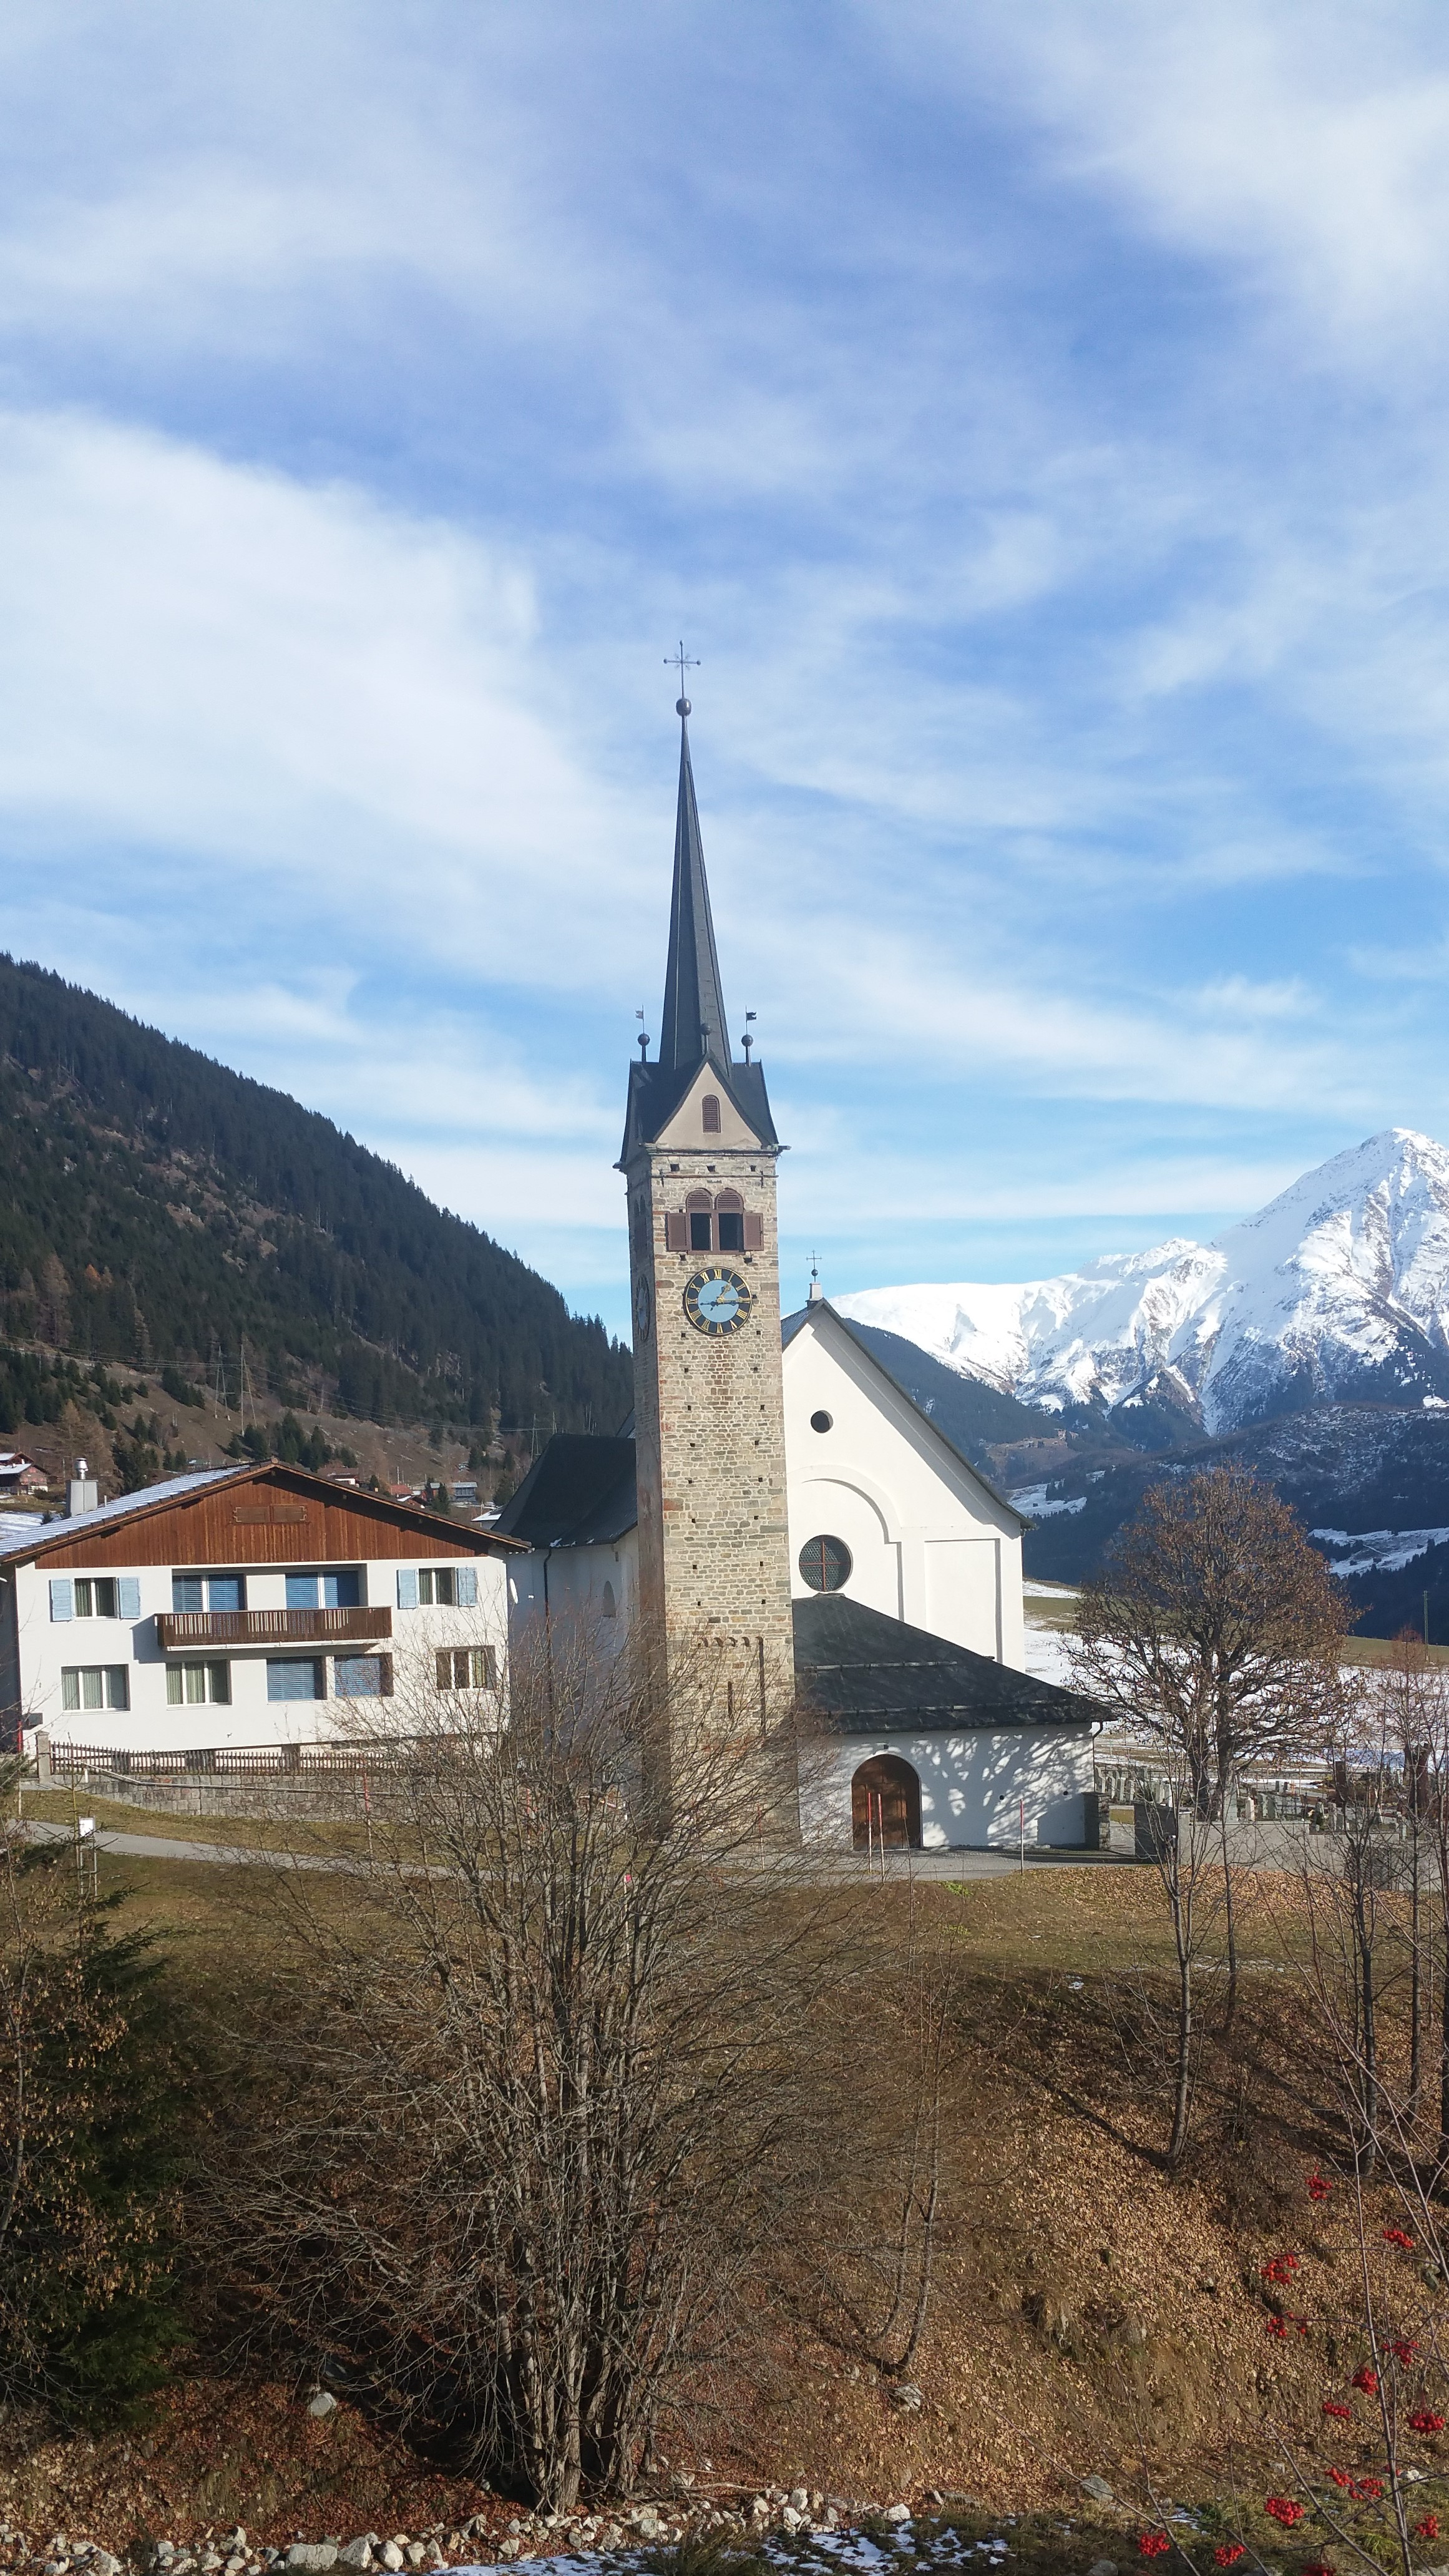
\includegraphics[angle=360,width=
	60mm]{figures/Baselgia da Sedrun.jpg}
	\caption{The church of Sedrun with its high tower}
\end{figure}

\begin{linenumbers}
\gll   Quèla blòca mávani ajn a tagliavan ò a trèvan vidò cun bùfs tòcan ò cò a Sadrùn. \\
 \textsc{dem.f.sg} block.\textsc{coll} go.\textsc{impf.3pl} up and cut.\textsc{impf.3pl} out and carry.\textsc{impf.3pl} down  with ox.\textsc{m.pl} until down here at \textsc{pn}  \\
\end{linenumbers}
\medskip
\glt `[With] these blocks they went up, cut [them] out, and brought them down with oxen until here in Sedrun.'
\medskip

\begin{linenumbers}
\gll   A pléndanajn in tòc da tschèla vart, lò ṣaj práctisch al sulèt grép da catschina tga végn avaun ála val Tujetsch. \\
and more\_uphill \textsc{indef.m.sg} piece of \textsc{dem.f.sg} side there \textsc{cop.prs.3sg} practically \textsc{def.m.sg} only.\textsc{m.sg} rock of limestone.\textsc{f.sg} \textsc{rel} come.\textsc{prs.3sg} before in.\textsc{def.f.sg} valley \textsc{pn}   \\
\end{linenumbers}
\medskip
\glt `And a little bit more uphill, a little bit on the other side, there is almost the only limestone rock that can be found in the Tujetsch valley.'
\medskip

\begin{linenumbers}
\gll Lò bagagjávani gjù catschina a barṣchavan grad èla.   \\
there build.\textsc{impf.3pl.3pl} down limestone.\textsc{f.sg} and  burn.\textsc{impf.3pl} immediately \textsc{3sg.f}\\
\end{linenumbers}
\medskip
\glt `There they would mine limestone and burn it immediately.'
\medskip

\begin{linenumbers}
\gll Ad i aun èra lò, zatgé rastònza ṣè aun lò tg’ ins sa í ajn a mirá; `l \textsc{pn} ò è fagj\footnotemark{} lò in pèr placats tga mùssan ajn via nùc’ ins sa è mirá quaj.\\
and \textsc{expl} still \textsc{exist.impf.3sg} there some remnant.\textsc{f.sg} \textsc{exist.prs.3sg} still there \textsc{rel} \textsc{gnr} can.\textsc{prs.3sg} go.\textsc{inf} into \textsc{subord} see.\textsc{inf} \textsc{def.m.sg} \textsc{pn} have.\textsc{prs.3sg} also make.\textsc{ptcp.unm} there \textsc{indef.m.sg} pair poster.\textsc{m.pl} \textsc{rel} show.\textsc{prs.3pl} in way where \textsc{gnr} can.\textsc{prs.3sg} also see.\textsc{inf} \textsc{dem.unm} \\
\end{linenumbers}
\medskip
\glt `And there were also, there still are some remnants there where one can go and see; \textsc{pn} also put some posters there which show where on the way one can have a look at this.'\footnotetext{The narrator thinks that \textit{tschentau} `put' would fit better than \textit{fatg}.}
\medskip

\begin{linenumbers}
\gll A lu Pr̩datsch … plénansé cò ancù̱ntar Tgòm … ṣaj ina rùsna, quaj fùṣ è aun intarassant sch’ ins savés, quaj datèscha da gl òn ju … a ùssa bigja grat prèsèn, méli a sistschian a zatgéj.   \\
and then \textsc{pn} {} more\_uphill here in\_direction \textsc{pn} {} \textsc{cop.prs.3sg.expl} \textsc{indef.f.sg} hole \textsc{dem.unm} \textsc{cop.cond.3sg} also indeed interesting.\textsc{unm} if \textsc{gnr} know.\textsc{cond.3sg} \textsc{dem.unm} date.\textsc{prs.3sg} from \textsc{def.m.sg} year \textsc{1sg} {} have.\textsc{prs.1sg} now \textsc{neg} just present thousand and six\_hundred and something\\
\end{linenumbers}
\medskip
\glt `And then Pardatsch … a bit more uphill here in direction of Tgom … there is a cave, it would indeed be interesting if one knew, this is dated, I … don't have it exactly in mind, sixteen hundred something.'
\medskip

\begin{linenumbers}
\gll  A lò pratjándani tga cavavan òra … matalts.  \\
and there pretend.\textsc{prs.3pl.3pl} \textsc{comp} recover.\textsc{impf.3pl} out {} metal.\textsc{m.pl}\\
\end{linenumbers}
\medskip
\glt `And there they pretend that they recovered metals.'
\medskip

\begin{linenumbers}
\gll A quaj è ina rùsna, òh tgé pù qual' èssar … in mè̱tar a miaz … lada, a fòrza … dus mè̱tars auta.   \\
and \textsc{dem.unm} \textsc{cop.prs.3sg} \textsc{indef.f.sg} hole oh what  can.\textsc{prs.3sg} \textsc{dem.f.sg} be.\textsc{inf} {} one.\textsc{m.sg} metre and half {} large.\textsc{f.sg} and maybe {} two.\textsc{m.pl} metre.\textsc{pl} high.\textsc{f.sg}\\
\end{linenumbers}
\medskip
\glt `And there is a cave, oh how big may it be …, one and a half metres … wide, and maybe … two metres high.'
\medskip

\begin{linenumbers}
\gll Daváuntiar ṣaj sé la, l’ anada cur' i òn antschiat, ad inṣ vèz’ aun quaj, bagagjávani gjù ... cun ah, bjè manuálmajn.   \\
in\_front  \textsc{cop.prs.3sg.expl} up \textsc{def.f.sg} \textsc{def.f.sg} year when \textsc{3pl} have.\textsc{prs.3pl} begin.\textsc{ptcp.unm} and \textsc{gnr}  see.\textsc{prs.3sg} still  \textsc{dem.unm} build.\textsc{impf.3pl.3pl} down {} with eh much manual.\textsc{adv}\\
\end{linenumbers}
\medskip
\glt `In front of it there is, eh, the year when they started, one can still see [that] they used to mine this with, ah, a lot manually.'
\medskip

\begin{linenumbers}
\gll Inṣ vèz’ aun tg’ èra dau vidajn pùntgas né trádals; sch’ i sitavan gljèz sau bétg.   \\
\textsc{gnr} see.\textsc{prs.3sg} still \textsc{comp} \textsc{pass.aux.impf.3sg} give.\textsc{ptcp.unm} into chisel.\textsc{f.pl} or power\_drill.\textsc{m.pl} whether \textsc{3pl} blow\_up.\textsc{impf.3pl} \textsc{dem.unm} know.\textsc{prs.1sg.1sg}  \textsc{neg}  \\
\end{linenumbers}
\medskip
\glt `One still can see that chisels or power drills had been used; whether they would blow up I don’t know.'
\medskip

\begin{linenumbers}
\gll A quèla tauna vò vidajn – quaj tgu sùn stauṣ ajn – vò lò vidajn circa véntgatschún mè̱tars, san inṣ\footnotemark {} í vidajn da quèla, api sasparti, vòi ajn duas.\\
and \textsc{dem.f.sg} cave go.\textsc{prs.3sg} into {}  \textsc{dem.unm} \textsc{rel.1sg} be.\textsc{prs.1sg} \textsc{cop.ptcp.m.sg} in {} go.\textsc{prs.3sg} there into about twenty-five metre.\textsc{m.pl} can.\textsc{prs.3sg} \textsc{gnr} go.\textsc{inf} into of \textsc{dem.f.sg} and \textsc{refl}.divide.\textsc{prs.3sg.expl} go.\textsc{prs.3sg.expl} in two.\textsc{f}  \\
\end{linenumbers}
\medskip
\glt `And this cave – [judging from] where I have been into it – one can go into it about 25 metres, and then it splits into two.'\footnotetext{\textit{san ins} is Standard Sursilvan for \textit{sò ins}.}
\medskip

\begin{linenumbers}
\gll   Ah, tgé ... prandèvan pròpi òra sa ins bégj' éxáct, dí dian ins matalṣ, ábar ò vèza quaj insùma bégj in grép da matal. \\
eh what {} take.\textsc{impf.3pl} exactly out know.\textsc{prs.3sg} \textsc{gnr} \textsc{neg} exact.\textsc{adj.unm} say.\textsc{inf} say.\textsc{prs.3sg} \textsc{gnr}  metal.\textsc{m.pl} but out look.\textsc{prs.3sg} \textsc{dem.unm} at\_all \textsc{neg} \textsc{indef.m.sg} rock.\textsc{m.sg} of metal.\textsc{m.sg}\\
\end{linenumbers}
\medskip
\glt `Ah, what … they really mined one does not know exactly, people say that it is metals, but this rock doesn't look like it contained metals at all.'
\medskip

\begin{linenumbers}
\gll Préndar ajn, pù schòn èssar tga samidav’ al grép, tga …  a dí di la … la détga di tg’ è̱rian schindanajn tg' i udé̱vian c’ i tucavi da mjadṣ-dé ajnt Ruèras.\\
take.\textsc{inf} in can.\textsc{prs.3sg} well be.\textsc{inf} \textsc{comp} \textsc{refl}.change.\textsc{impf.3sg} \textsc{def.m.sg} rock \textsc{comp} {} and say.\textsc{inf} say.\textsc{prs.3sg} \textsc{def.f.sg} {} \textsc{def.f.sg} legend say.\textsc{prs.3sg}  \textsc{comp} \textsc{cop.impf.sbjv.3pl} so\_in \textsc{comp} \textsc{3pl} hear.\textsc{impf.sbjv.3pl} \textsc{subord} \textsc{expl} beat.\textsc{impf.sbjv.3sg} of noon.\textsc{m.sg} in \textsc{pn}\\
\end{linenumbers}
\medskip
\glt `As for mining, it could well be that the rock changed, that …, the legend says that they were so deep in the cave that they heard the clock strike noon in Rueras.'
\medskip

\begin{linenumbers}
\gll  Quaj è da dubitá, quaj è mataj scù quaj tga … i dat aun bjè da quèlas détgas.  \\
 \textsc{dem.unm}  \textsc{cop.prs.3sg} \textsc{comp} doubt.\textsc{inf} \textsc{dem.unm} \textsc{cop.prs.3sg} probably like \textsc{dem.unm} \textsc{rel} {} \textsc{expl} \textsc{exist.prs.3sg} still many of \textsc{dem.f.pl} legend.\textsc{pl} \\
\end{linenumbers}
\medskip
\glt `This, one has to doubt, this is probably like what … there still are many such legends.'
\medskip

\begin{linenumbers}
\gll   Basta, ah, par vagní cò sén quaj Pardatsch al, al tat vèva aun fatg ina satagljèda, ina ganùglja vèva `l tagljau sé, schòn, in braf schnéz; avaun c’ í vidajn, ah, staus lu tial miadi, gljèz èra lu bitg in, ah, schi sémpal da dumagnè tiar in miadi. \\
enough eh \textsc{subord} come.\textsc{inf} here on \textsc{dem.unm} \textsc{pn} \textsc{def.m.sg} \textsc{def.m.sg} grandfather have.\textsc{impf.3sg} in\_addition make.\textsc{ptcp.unm} \textsc{indef.f.sg} \textsc{refl.}cut.\textsc{ptcp.f.sg} \textsc{indef.f.sg} knee have.\textsc{impf.3sg} \textsc{3sg.m} cut.\textsc{ptcp.unm} up yes \textsc{indef.m.sg} brave.\textsc{m.sg.unm} cut.\textsc{m.sg} before \textsc{} go.\textsc{inf} uphill eh \textsc{cop.ptcp.m.sg} then  at.\textsc{def.m.sg} doctor \textsc{dem.unm} \textsc{cop.impf.3sg} then \textsc{neg} \textsc{indef.m.sg} eh so simple.\textsc{adj.unm} \textsc{comp} cope\_with.\textsc{inf} at \textsc{indef.m.sg} doctor\\
\end{linenumbers}
\medskip
\glt `Enough, eh, in order to come back to Pardatsch, my grandfather, in addition, had had a cut, he cut his knee, yes, an important cut; before going uphill, eh [he] went to the doctor but this was not eh easy to deal with at the doctor’s.'
\medskip

\begin{linenumbers}
\gll  Lèdṣ vèva lu dau zatgéj étg dad úndṣchar ajn a faschas a la tata ò lu aun détg da mé:  \\
 \textsc{dem.m.sg} have.\textsc{impf.3sg} then  give.\textsc{ptcp.unm} some ointment.\textsc{m.sg} \textsc{attr} oil.\textsc{inf} in and bandage.\textsc{f.pl} and \textsc{def.f.sg} grandmother have.\textsc{prs.3sg} then still say.\textsc{ptcp.unm} \textsc{dat} \textsc{1sg}  \\
\end{linenumbers}
\medskip
\glt `He had given [him] some ointment to rub in and bandages, and then my grandmother said to me:'
\medskip

\begin{linenumbers}
\gll  «Té mira lu tg’ al tat fétschi lu mintga dé, prèndi gjù quaj a ṣchubrègi a fétschi sé da néjf.»  \\
 \textsc{2sg} look.\textsc{imp.2sg} then \textsc{comp} \textsc{def.m.sg} grandfather do.\textsc{prs.sbjv.3sg} then every.\textsc{m.sg} day take.\textsc{prs.sbjv.3sg} down \textsc{dem.unm} and clean.\textsc{prs.sbjv.3sg} and do.\textsc{prs.sbjv.3sg} up of new.\textsc{adj.unm} \\
\end{linenumbers}
\medskip
\glt `And you, make sure that your grandfather does it every day, that he takes them off, that he cleans them and puts them on again.'
\medskip

\begin{linenumbers}
\gll  «Gè gè gè quaj vi ju schòn … mirá tga végni fatg.»  \\
yes yes yes  \textsc{dem.unm} want.\textsc{prs.1sg} \textsc{1sg} of\_course {}  make\_sure.\textsc{inf} \textsc{comp} \textsc{pass.aux.prs.sbjv.3sg} do.\textsc{ptcp.unm}   \\
\end{linenumbers}
\medskip
\glt `Yes of course, I will make sure that it's be done.'
\medskip

\begin{linenumbers}
\gll  A … grat par finí quèla istòrja, qu’ è lu ju ... quèluísa, ju ṣchèva mintgataun dal tat:  \\
and {} just  \textsc{subord} end.\textsc{inf} \textsc{dem.f.sg} story \textsc{dem.unm} be.\textsc{prs.3sg} then go.\textsc{ptcp.unm} {} so \textsc{1sg} say.\textsc{impf.1sg}  sometimes \textsc{dat} grandfather.\textsc{m.sg} \\
\end{linenumbers}
\medskip
\glt `And … in order to conclude this story, it went in the following way: I said from time to time to my grandfather:'
\medskip

\begin{linenumbers}
\gll «Té\footnotemark{} … Vajs fatg èl?»   \\
 \textsc{2sg} {} have.\textsc{prs.2sg.pol} do.\textsc{ptcp.unm} \textsc{3sg.m}\\
\end{linenumbers}
\medskip
\glt `You [sg] ... Did you [pl] do it?'\footnotetext{The narrator makes an error; he said \textit{té} ‘you (sg)’ instead of \textit{Vus} ‘you (honorific)’, as the following sentence explains.}
\medskip

\begin{linenumbers}
\gll  Lu ṣchèv’ inṣ aun Vuṣ da ... ah, da tat a tata vau adina détg Vuṣ, ábar dals, méjs gjaniturs ... vajn nuṣ ùssa bégja détg Vus, ábar i èra bjèrs tga … òn détg tòcan, gè práctiṣch adina Vus dals gjaniturs.  \\
then say.\textsc{impf.3sg} \textsc{gnr} still  \textsc{2pl} \textsc{dat} {} eh \textsc{dat} grandfather.\textsc{m.sg} and grandmother.\textsc{f.sg} have.\textsc{prs.1sg.1sg} always say.\textsc{ptcp.unm} \textsc{2pl.pol} but \textsc{dat.def.m.pl} \textsc{poss.1sg.m.pl} parent.\textsc{pl} {} have.\textsc{prs.1pl} \textsc{1pl} now \textsc{neg} say.\textsc{ptcp.unm} \textsc{2pl.pol} but \textsc{expl} \textsc{exist.impf.3sg} many.\textsc{m.pl} \textsc{rel} {} have.\textsc{prs.3pl} say.\textsc{ptcp.unm} until yes practically always \textsc{2pl} \textsc{dat.def.m.pl} parent.\textsc{pl}\\
\end{linenumbers}
\medskip
\glt `At that time, one used to say \textit{Vus} to ... eh, to my grandfather and my grandmother I have always said \textit{Vus}, but to the, my parents ... we now never said \textit{Vus}, but there were many who have said until, well practically always \textit{Vus} to their parents.'
\medskip

\begin{linenumbers}
\gll  [Lu] vòu détg:  «Vuṣ vèssas lu aun da fá quèls bògns né mirá da la plaja.»  \\
then have.\textsc{prs.1sg.1sg} say.\textsc{ptcp.unm} \textsc{2pl.pol}  have.\textsc{cond.2pl} then still to  do.\textsc{inf} \textsc{dem.m.pl} bath.\textsc{pl} or look\_after.\textsc{inf} of \textsc{def.f.sg} wound\\
\end{linenumbers}
\medskip
\glt `[Then] I said: "You should still take a bath or look after the wound."'
\medskip

\begin{linenumbers}
\gll  «Gè gè quaj è schòn bian.»  \\
yes yes \textsc{dem.unm} \textsc{cop.prs.3sg} all\_right good.\textsc{unm}  \\
\end{linenumbers}
\medskip
\glt `Yes, sure, that’s OK.'
\medskip

\begin{linenumbers}
\gll  Qu' è lu ju quèluísa tga ca nuṣ èssan vagní vidòra, turnaj ò da Pardatsch, tg' èssan nus staj ajn lò fòrsa … quátar tschun jamnas.  \\
 \textsc{dem.unm} be.\textsc{prs.3sg} then go.\textsc{ptcp.unm} \textsc{dem}\_way \textsc{rel} \textsc{rel} \textsc{1pl} be.\textsc{impf.1pl} come.\textsc{ptcp.m.pl} over\_out return.\textsc{ptcp.m.pl} out of \textsc{pn} \textsc{corr} be.\textsc{cond.1pl} \textsc{1pl} \textsc{cop.ptcp.m.pl} in there maybe {} four five week.\textsc{f.pl}   \\
\end{linenumbers}
\medskip
\glt `This happened in such a way that when we returned down [to Surrein] from Pardatsch, then we had stayed there maybe … four or five weeks.'
\medskip

\begin{linenumbers}
\gll  Scha vèva `l fatg ṣchùber nuét.  \\
but have.\textsc{impf.3sg} \textsc{3sg.m} do.\textsc{ptcp.unm} clean.\textsc{adj.unm} nothing \\
\end{linenumbers}
\medskip
\glt `But he hadn’t done anything at all.'
\medskip

\begin{linenumbers}
\gll Quèla fascha èra satratg’ anzjaman, a vidajn ála pjal, carschid’ ajn ála pjal api ò `l stju í ò tial dòctar.  \\
\textsc{dem.f.sg} bandage be.\textsc{impf.3sg} \textsc{refl.}contract.\textsc{impf.3sg} together and into to.\textsc{def.f.sg} skin grow.\textsc{ptcp.f.sg} in in.\textsc{def.f.sg} skin and have.\textsc{prs.3sg} \textsc{3sg.m} must.\textsc{ptcp.unm} go.\textsc{inf} out to.\textsc{def.m.sg} doctor \\
\end{linenumbers}
\medskip
\glt `That bandage had contracted, and into the skin, grown into the skin and then he had to go to the doctor.'
\medskip

\begin{linenumbers}
\gll  Ábar èl vèva par clétg fétg bian saun al … ò `l lu nuéta gju còmplicazjuns.  \\
but  \textsc{3sg.m} have.\textsc{impf.3sg} for luck.\textsc{m.sg} very good.\textsc{m.sg.unm} blood \textsc{def.m.sg} {} have.\textsc{prs.3sg} \textsc{3sg.m} then \textsc{neg} have.\textsc{ptcp.unm} complication.\textsc{f.sg}\\
\end{linenumbers}
\medskip
\glt `But fortunately his blood was very good, the … he then hadn’t got any complications.'
\medskip

\begin{linenumbers}
\gll  Ajnta Pardadṣch vèvan nus circa déjsch, èba déjsch quéndisch tgauṣ grònṣ api vèvan nus tgauraṣ a pòrs.  \\
up\_in \textsc{pn} have.\textsc{impf.1pl} \textsc{1pl} about ten precisely ten fifteen head.\textsc{m.pl} big.\textsc{pl} and have.\textsc{impf.1pl} \textsc{1pl} goat.\textsc{f.pl} and pig.\textsc{m.pl} \\
\end{linenumbers}
\medskip
\glt `Up in Pardatsch we had about ten, as already mentioned ten or fifteen large farm animals, and we had [also] goats and pigs.'
\medskip

\begin{linenumbers}
\gll A lu mia lavur èra ... èra bitga atgnamajn da fá bjè, a quaj tg’ èra da parvaj aun djantarájn fagèv’ al tat, api vèvanṣ da partgirá als tiars, mav’ ins lò sédòr ál sit, grat cò nùca quèla rùsna tgu a raquintau.\\
and then \textsc{poss.1sg.f.sg} work \textsc{cop.impf.3sg} {} \textsc{cop.impf.3sg} \textsc{neg} actually \textsc{attr} do.\textsc{inf} much and \textsc{dem.unm} \textsc{rel} be.\textsc{impf.3sg} to feed.\textsc{inf} still in\_between do.\textsc{impf.3sg} \textsc{def.m.sg} grandfather, and have.\textsc{impf.1pl.1pl} to mind.\textsc{inf} \textsc{def.m.pl} animal.\textsc{pl} go.\textsc{impf.3sg} \textsc{gnr} there up\_out in.\textsc{def.m.sg} south just there by \textsc{dem.f.sg} hole \textsc{rel.1sg} have.\textsc{prs.1sg} tell.\textsc{ptcp.unm}\\  
\end{linenumbers}
\medskip
\glt `And my work was, was ... not exactly to do a lot, and what still had to be fed in between, my grandfather would do, and we also had to mind the animals; we would then go up to the south, just by that cave I have mentioned.'
\medskip

\begin{linenumbers}
\gll  Lò èr’ inṣ bjè culs tiars, a ... la sèra vagní gjùdòra cun èls, a lu al tat, lèz pinava tiar la tschajna, gljèz èra magari è léjgar tgé cuṣchinadaṣ èl [fagèva], èl cuṣchinava bitga mal, ábar ah mintgataun fagèva `l schòn détgs, détgas pistracas.\\
there \textsc{cop.impf.3sg} \textsc{gnr} a\_lot  with.\textsc{def.m.pl} animal.\textsc{pl} and {} \textsc{def.f.sg} evening  come.\textsc{ptcp.m.pl} down\_out with \textsc{3pl.m} and then \textsc{def.m.sg} grandfather \textsc{dem.m.sg} prepare.\textsc{impf.3sg} by \textsc{def.f.sg} dinner \textsc{dem.unm} \textsc{cop.impf.3sg} sometimes also funny.\textsc{adj.unm} what cook.\textsc{ptcp.f.pl} \textsc{3sg.m} [make.\textsc{impf.3sg}] \textsc{3sg.m} cook.\textsc{impf.3sg} \textsc{neg} bad but ah sometimes make.\textsc{impf} \textsc{3sg.m} really real.\textsc{m.pl} real.\textsc{f.pl} mixture.\textsc{pl}\\
\end{linenumbers}
\medskip
\glt `There we were often with the animals, and ... in the evening we would come back with them, and then my grandfather, he would prepare dinner, it was sometimes also funny [to see] what he [cooked], he didn’t cook badly, but ah from time to time he would prepare terrible mixtures.'
\medskip

\begin{linenumbers}
\gll  Quaj sch’ i dèva rèsts, scha vagnévi lu magari rimnau quaj dus trajs diṣ api méz tùt ajn ina … tùt anzjaman.  \\
well if \textsc{expl} \textsc{exist.impf.3sg} leftovers.\textsc{m.pl} then \textsc{pass.aux.impf.3sg.expl} then sometimes collect.\textsc{ptcp.unm} \textsc{dem.unm} two.\textsc{m.pl} three day.\textsc{pl} and put.\textsc{ptcp.unm} all in  \textsc{indef.f.sg} {} all together\\
\end{linenumbers} 
\medskip
\glt `Well, when there were leftovers, they would sometimes be collected for two or three days and then put all together in a … all together.'
\medskip

\begin{linenumbers}
\gll A sjantar tschajnas, gljèz, quaj èra schòn è aun léjgar.   \\
and after dinner.\textsc{f.pl} \textsc{dem.unm} \textsc{dem.unm} \textsc{cop.impf.3sg} really also still funny.\textsc{adj.unm}  \\
\end{linenumbers}
\medskip
\glt `And after dinner, well, this was also funny.'
\medskip

\begin{linenumbers}
\gll  Sjantar tschajna mav’ inṣ ajn, quaj èr’ èr, èls èran rèligjúṣ, èra quaj nùndétg. \\
after dinner.\textsc{f.sg} go.\textsc{impf.3sg} \textsc{gnr} in \textsc{dem.unm} \textsc{cop.impf.3sg} also \textsc{3pl.m} \textsc{cop.impf.3pl} religious.\textsc{m.pl} \textsc{cop.impf.3sg} \textsc{dem.unm} indescribable.\textsc{adj.unm}\\
\end{linenumbers}
\medskip
\glt `After dinner we would go in, this was also, they were religious, this was indescribable.'
\medskip

\begin{linenumbers}
\gll  Vagnévi ju ajn ajn nuégl, parquaj tga … l’ antschata da la parmavèra stuèv’ ins schè ajn als tiarṣ ajn nuégl, a lu máv’ inṣ ajn api ṣchèva `l:   \\
 come.\textsc{impf.3sg.expl} go.\textsc{ptcp.unm} in in barn because \textsc{subord} {} \textsc{def.f.sg} beginning of \textsc{def.f.sg} spring must.\textsc{impf.3sg} \textsc{gnr} let.\textsc{inf} in \textsc{def.m.pl} animal.\textsc{pl} in barn.\textsc{m.sg} and then go.\textsc{impf.3sg} \textsc{gnr} in and say.\textsc{impf.3sg} \textsc{3sg.m}\\
\end{linenumbers}
\medskip
\glt `When they entered the barn, because … at the beginning of spring one had to let the animals into the barn, and then one would enter and then he would say:'
\medskip

\begin{linenumbers}
\gll  «Sò, ùsa ṣchajn nuṣ impau patarnòṣ.» ad èl samatév’ adina giùdajn.  \\
OK now say.\textsc{prs.1pl} \textsc{1pl} a\_bit  Lord’s\_prayer.\textsc{m.pl} and \textsc{3sg.m} \textsc{refl}.put.\textsc{impf.3sg} always down\_in  \\
\end{linenumbers}
\medskip
\glt `«OK, now we will say some Lord’s prayer» and he would always sit down in [a manger].'
\medskip

\begin{linenumbers}
\gll Suschéa sasév’ ajn ajn purṣèpan, a … èl dad ina vart ad ju da tschèla vart, a quaj ṣchèva `l trajs quátar  patarnòṣ a vònzaj èri «Sòntga Maria Mùma da Dju» api èra `l navèn.\\
exactly\_so sit.\textsc{impf.3sg} in in manger and {} \textsc{3sg.m} of \textsc{indef.f.sg} side and \textsc{1sg} of \textsc{dem.f.sg} side and \textsc{dem.unm} say.\textsc{impf.3sg} \textsc{3sg.m} three four Lord’s\_prayer.\textsc{m.pl} and later \textsc{cop.impf.3sg.expl} Holy Mary Mother of God and \textsc{cop.impf.3sg} \textsc{3sg.m} away\\
\end{linenumbers}
\medskip
\glt `So he would sit in the manger, and … he on the one side and I on the other side, and so he would say three or four Lord’s prayers and a bit later «Holy Mary Mother of God», and then he was gone.'
\medskip

\begin{linenumbers}
\gll  Sadurmantav’ ajn. A lu dumagnav’ ju bigja nònavaun èl.  \\
 \textsc{refl}.fall\_asleep.\textsc{impf.3sg} in and then induce.\textsc{impf.1sg} \textsc{1sg} \textsc{neg} awake \textsc{3sg.m}\\
\end{linenumbers}
\medskip
\glt `He would fall asleep. And  then I wasn't able to wake him up.'
\medskip

\begin{linenumbers}
\gll  Quèl durméva sc’ in tajs.  \\
 \textsc{dem.m.sg} sleep.\textsc{impf.3sg} like \textsc{indef.m.sg} badger\\
\end{linenumbers}
\medskip
\glt `He used to sleep like a log.'
\medskip

\begin{linenumbers}
\gll Ṣùtajn èri la tégja nùca `l caṣchav' èra, daspèras quèls dus nuégls api stuèv' inṣ í ò ad í sé sén clavau, a lò èri ajn ina stiva sc’ ins ṣchèva, ajn quèls majṣès ṣchèv’ ins la stiva nùc’ ins durméva.\\
under\_in \textsc{cop.impf.3sg.expl} \textsc{def.f.sg} alpine\_hut \textsc{rel} \textsc{3sg.m} make\_cheese.\textsc{impf.3sg} also next \textsc{dem.m.pl} two.\textsc{m} cow\_barn.\textsc{pl} and must.\textsc{impf.3sg} \textsc{gnr} go.\textsc{inf} out and go.\textsc{inf} up upon hay\_barn.\textsc{m.sg} and there \textsc{cop.impf.3sg.expl} in \textsc{def.f.sg} living\_room as \textsc{gnr} say.\textsc{impf.3sg} in \textsc{dem.m.pl} assembly\_of\_houses.\textsc{pl} say.\textsc{impf.3sg} \textsc{gnr} \textsc{def.f.sg} living\_room  \textsc{rel.loc} \textsc{gnr} sleep.\textsc{impf.3sg}\\
\end{linenumbers}
\medskip
\glt `Below was the alpine hut where he would also make cheese, next to it those two cow barns and one must go out and up into the hay barn, and therein was the \textit{stiva}, the living room, as they used to say, in those \textit{majṣés} the room where one slept was called \textit{stiva}.'
\medskip

\begin{linenumbers}
\gll  Ad ju mava lu sé lò durmí, ábar ah, bjè nòtgs staus parsuls sé lò, ha, a lò vòu schòn ah … gju inqual tèma.   \\
and \textsc{1sg} go.\textsc{impf.1sg} then up there sleep.\textsc{inf} but eh many night.\textsc{f.pl} \textsc{cop.ptcp.m.sg} alone.\textsc{m.sg} up there ha and there have.\textsc{prs.1sg.1sg} really eh {} have.\textsc{ptcp.unm} some fear.\textsc{f.sg} \\
\end{linenumbers}
\medskip
\glt `And I used to go up there to sleep, but, eh, many nights I was alone up there, ha, and there I was eh sometimes afraid.'
\medskip

\begin{linenumbers}
\gll  Ajn quèla végljadé̱tgna, api al pròblè̱m èra, èra, al pròblè̱m èra las sòndaṣ a dumèngjas.   \\
in  \textsc{dem.f.sg} age and \textsc{def.m.sg} problem \textsc{cop.impf.3sg} \textsc{cop.impf.3sg} \textsc{def.m.sg} problem \textsc{cop.impf.3sg} \textsc{def.f.pl} Saturday.\textsc{pl} and Sunday.\textsc{pl} \\
\end{linenumbers}
\medskip
\glt `At that age, and the problem was, was, the problem was on Saturdays and Sundays.'
\medskip

\begin{linenumbers}
\gll Né al vèndardís sèra, quèls taljans, quaj èra práctisch mù taljans tga luvravan cò vid la via. \\
or \textsc{def.m.sg} Friday evening.\textsc{f.sg} \textsc{dem.m.pl} Italian.\textsc{pl} \textsc{dem.unm} \textsc{cop.impf.3sg}  practically only Italian.\textsc{m.pl} \textsc{rel} work.\textsc{impf.3pl} here at \textsc{def.f.sg} road  \\
\end{linenumbers}
\medskip
\glt `Or Friday evening, these Italians, there were practically only Italians who worked on the road.'
\medskip

\begin{linenumbers}
\gll  Sé Nalps vèvani è grad antschiat a bagagè cantinaṣ ètcè̱tara.\\
up \textsc{pn} have.\textsc{impf.3pl.3pl} also just start.\textsc{ptcp.unm} \textsc{comp} build.\textsc{inf} canteen.\textsc{f.pl} et\_cetera\\
\end{linenumbers}
\medskip
\glt `In Nalps they had just begun to build canteens and so on.'
\medskip

\begin{linenumbers}
\gll Sònda-dumèngja vagnévan quèls ò cò a fagjèvan fjastunas.\\
Saturday-Sunday come.\textsc{impf.3pl} \textsc{dem.m.pl} out here and do.\textsc{impf.3pl} party.\textsc{augm.f.pl}\\
\end{linenumbers}
\medskip
\glt `On week-ends they would come here and have big parties.'
\medskip

\begin{linenumbers}
\gll A  magari tga pudèvan lu bigja … vidajn a ... vajn gju in pèr jèdas quèls tga vagnévan, u tga vagnévan ajn ál clavau a durmévan, ábar è ál légj dal tat ... sùnd ju è schòn sadastadaus tg' i èr' ajn ... in né dus taljánars tga durmévan.\\
and sometimes  \textsc{subord} can.\textsc{impf.3pl} then \textsc{neg} {} in and {} have.\textsc{prs.1sg} have.\textsc{ptcp.unm} \textsc{indef.m.sg} pair  time.\textsc{f.pl} \textsc{dem.m.pl} \textsc{rel} come.\textsc{impf.3pl} or \textsc{rel} come.\textsc{impf.3pl} in in.\textsc{def.m.sg} barn and sleep.\textsc{impf.3pl} but also in.\textsc{def.m.sg} bed of.\textsc{def.m.sg} grandfather {} be.\textsc{prs.1sg} \textsc{1sg} also already \textsc{refl.}wake\_up.\textsc{ptcp.m.sg} \textsc{rel} \textsc{expl} \textsc{cop.impf.3sg} in {} one.\textsc{m.sg} or two.\textsc{m.pl} Italian.\textsc{pl} \textsc{rel} sleep.\textsc{impf.3pl}  \\
\end{linenumbers}
\medskip
\glt `Now sometimes they couldn’t manage ... to come … into [the \textit{stiva} and sleep on hay] and … we sometimes had those who came or who came into the barn and slept [there], but I happened to wake up there when one or two Italians were sleeping [in my grandfather’s bed].'
\medskip

\begin{linenumbers}
\gll  Òh, lu schòn tumju in pau mintgataun.  \\
oh then really be\_afraid.\textsc{ptcp.unm} \textsc{indef.m.sg} little sometimes  \\
\end{linenumbers}
\medskip
\glt `Oh, [I was] really afraid sometimes.'
\medskip

\begin{linenumbers}
\gll  Pr̩quaj tga quaj c’ ins ... vèva bigja grad da partgirá tiars sch’ èr’ inṣ antir dé cun quèls, qu' èra è intarassant da mirá c’ i luvravan, c' i bagagjavan gjù.  \\
because \textsc{subord} \textsc{dem.unm} when \textsc{gnr} {} have.\textsc{impf.3sg}  \textsc{neg} just to mind.\textsc{inf} animal.\textsc{m.pl} then \textsc{cop.impf.3sg} \textsc{gnr} whole.\textsc{m.sg} day with \textsc{dem.m.pl} \textsc{dem.unm} \textsc{cop.impf.3sg} also interesting.\textsc{adj.unm} \textsc{mod} look.\textsc{inf} when \textsc{3pl} work.\textsc{impf.3pl} when \textsc{3pl} build.\textsc{impf.3sg} down\\
\end{linenumbers}
\medskip
\glt `Because when we ... didn’t just have to mind the animals, we were with them [the Italian workers] the whole day; it was also interesting to watch [them] when they were working, when they would dismantle [something].'
\medskip

\begin{linenumbers}
\gll  Ò lò vòu fòrza schòn è survagnú in téc quajda d' í par crapa, tgu a vju difarènts lògans tg’ i vèvan sitau gjù ad èra … vagnú ò cristalaṣ ètcè̱tara, tga quaj è fòrza schòn stau in téc al … mòtif tgu a antschiat dad í par crapa.   \\
out there  have.\textsc{prs.1sg.1sg} maybe really also get.\textsc{ptcp.unm} \textsc{indef.m.sg} bit desire.\textsc{f.sg} \textsc{attr} go.\textsc{inf} for stone.\textsc{coll} \textsc{rel.1sg} have.\textsc{prs.1sg} see.\textsc{ptcp.unm} different.\textsc{m.pl} place.\textsc{pl} \textsc{rel} \textsc{3pl} have.\textsc{impf.3pl} blast.\textsc{ptcp.unm} down and be.\textsc{impf.3sg} {} come.\textsc{ptcp.unm} out crystal.\textsc{f.pl} et\_cetera \textsc{comp} \textsc{dem.unm} be.\textsc{prs.3sg} maybe really  \textsc{cop.ptcp.unm} \textsc{indef.m.sg} bit \textsc{def.m.sg} {} reason \textsc{rel.1sg} have.\textsc{prs.1sg} begin.\textsc{ptcp.unm} \textsc{comp} go.\textsc{inf} for stone.\textsc{coll}\\
\end{linenumbers}
\medskip
\glt `Out there I might have started enjoying looking for stones a bit, when I saw different places where they had blasted [the rocks], and crystals and so forth … had come out, so maybe this has been a bit the reason why I began to go for stones. '
\medskip

\begin{linenumbers}
\gll Schabi tga lu, cun siṣ òns capév’ ins hald aun mèmja pauc a vèva bigja la ... fòrsa da fá zatgéj.   \\
although \textsc{subord} then with six year.\textsc{m.pl} understand.\textsc{impf.3sg} \textsc{gnr} just still too little and have.\textsc{impf.3sg} \textsc{neg} \textsc{def.f.sg} {} strength \textsc{attr} do.\textsc{inf} something\\
\end{linenumbers}
\medskip
\glt `Although then, at the age of six, one would understand too little and wouldn’t have the ... strength to do something.'
\medskip

\begin{linenumbers}
\gll  Gè, ah … cèrtas tgaussas al tat, lèz al dé òra mava lu bjè par lèna a mava lu vidòra in tòc a pinava ògna, a vagnéva vidajn ... tg’ èl mava a rimnava, gljèz èra aun léjgar cu ’l scarpava gjù urticlas.  \\
yes eh {} certain.\textsc{f.pl} thing.\textsc{pl} \textsc{def.m.sg} grandfather \textsc{dem.m.sg}  \textsc{def.m.sg} day out go.\textsc{impf.3sg} then often for wood.\textsc{coll} and go.\textsc{impf.3sg} then over\_out \textsc{def.m.sg} piece and prepare.\textsc{impf.3sg} alder.\textsc{coll} and come.\textsc{impf.3sg} over\_in {} \textsc{rel} \textsc{3sg.m} go.\textsc{impf.3sg} and collect.\textsc{impf.3sg} \textsc{dem.unm} \textsc{cop.impf.3sg} really funny.\textsc{adj.unm} when \textsc{3sg.m} pull\_off.\textsc{impf.3sg} down nettle.\textsc{f.pl} \\
\end{linenumbers}
\medskip
\glt `Yes, ah, certain things my grandfather, he would often look for wood the whole day, and he would then go down a little bit and log alder, and when he was coming up ... when he would go and collect it, that was really funny when he pulled off nettles.'
\medskip

\begin{linenumbers}
\gll   Quaj duvrava `l par dá dis pòrs, trúfals ansjaman par dá áls pòrs. \\
 \textsc{dem.unm} use.\textsc{impf.3sg} \textsc{3sg.m} \textsc{subord} give.\textsc{inf} \textsc{def.dat.pl} pig.\textsc{m.pl} potato.\textsc{m.pl} together \textsc{subord} give.\textsc{inf} \textsc{dat.def.m.pl} pig.\textsc{pl}\\
\end{linenumbers}
\medskip
\glt `This he used to give the pigs, potatoes together [with nettles] to give the pigs.'
\medskip

\begin{linenumbers}
\gll  Ah, quaj scarpava `l adina cul maun, cul maun sènza [vòns].  \\
ah  \textsc{dem.unm} pull\_off.\textsc{impf.3sg} \textsc{3sg.m} always with.\textsc{def.m.sg} hand with.\textsc{def.m.sg} hand without [glove.\textsc{m.pl}]  \\
\end{linenumbers}
\medskip
\glt `Ah, and the nettles, he would always pull them down with the hand, with the hand without [gloves].'
\medskip

\begin{linenumbers}
\gll  Ju tartgava quaj è bitga pussajval.  \\
 \textsc{1sg} think.\textsc{impf.1sg} \textsc{dem.unm} \textsc{cop.prs.3sg} \textsc{neg} possible.\textsc{adj.unm}  \\ 
\end{linenumbers} 
\medskip
\glt `I thought that this was not possible.'
\medskip

\begin{linenumbers}
\gll  Ad è zatgéj ... léjgar èr’ èra cu 'l fagèva fjuc.  \\
 and also something {} funny.\textsc{adj.unm} \textsc{cop.impf.3sg} also when \textsc{3sg.m} make.\textsc{impf.3sg} fire.\textsc{m.sg} \\
\end{linenumbers}
\medskip
\glt `And something ... funny was also when he made fire.'
\medskip

\begin{linenumbers}
\gll Èl vèv’ adina … lèna vèva `l dètg avùnda, ábar ajn gé̱néral vagnévi bitga fatg òra. \\
 \textsc{3sg.m} have.\textsc{impf.3sg} always {} wood.\textsc{coll} have.\textsc{impf.3sg} \textsc{3sg.m} much enough but in general \textsc{pass.aux.impf.3sg.expl} \textsc{neg} make.\textsc{ptcp.unm} out  \\
\end{linenumbers}
\medskip
\glt `He had always … wood, he  had enough, but it was generally not split.'
\medskip

\begin{linenumbers}
\gll  Quaj èra magari da quèls pléjdars dad in mèter dus, ùs ussusché. \\
 \textsc{dem.unm} \textsc{cop.impf.3sg} sometimes of \textsc{dem.m.pl} block.\textsc{pl} of one.\textsc{m.sg} metre two.\textsc{m.p}l now exactly\_so  \\
\end{linenumbers}
\medskip
\glt `These were sometimes such blocks of one or two metres or so.'
\medskip

\begin{linenumbers}
\gll Quaj catschava `l ajn, qu’ èr’ in plantschju da … da taratsch naturálmajn.\\
 \textsc{dem.unm} throw.\textsc{impf.3sg} \textsc{3sg.m} in \textsc{dem.unm} \textsc{cop.impf.3sg} \textsc{indef.m.sg} floor of {} of soil.\textsc{m.sg} natural.\textsc{adv}\\
\end{linenumbers}
\medskip
\glt `This he would throw into [the fire], this was a floor of … of soil, of course.'
\medskip

\begin{linenumbers}
\gll Quaj catschava `l vidajn ála fuajna api mù catschava sjantar mintg’ jèda.\\
 \textsc{dem.unm} throw.\textsc{impf.3sg} \textsc{3sg.m} into in.\textsc{def.f.sg} fireplace and only throw.\textsc{impf.3sg} after every.\textsc{f.sg} time\\
\end{linenumbers}
\medskip
\glt `That is what he used to throw into the fireplace and he used to throw in more every time.'
\medskip
 
\begin{linenumbers}
\gll  A la sèra par tga briṣchi bétg … vagnéva quaj, quaj mava `l ajnagjù cul maun èra sènza … [vòns] a trèva vidò̱ còtgla gjù sé sél plantschju.  \\
and \textsc{def.f.sg} evening  for \textsc{subord} burn.\textsc{prs.sbjv.3sg} \textsc{neg} {} \textsc{pass.aux.impf.3sg} \textsc{dem.unm} \textsc{dem.unm} go.\textsc{impf.3sg} \textsc{3sg.m} in\_down with.\textsc{def.m.sg} hand also without {} [glove.\textsc{m.pl}] and pull.\textsc{impf.3sg} out charcoal.\textsc{coll} down up on.\textsc{def.m.sg} floor  \\
\end{linenumbers}
\medskip
\glt `And in the evening, to avoid it burning … was that, there he went into [the fire] with one hand, also without [gloves], and pulled out charcoal from down there up to the floor.'
\medskip

\begin{linenumbers}
\gll Álṣò i èra schòn in in spazjal.    \\
well \textsc{expl} \textsc{cop.impf.3sg} really \textsc{indef.m.sg} \textsc{indef.m.sg} special.\textsc{adj.unm} \\
\end{linenumbers}
\medskip
\glt `Well, he really was a special person.'
\medskip 

\begin{linenumbers}
\gll  A bjè gljut tumévan è mju tat, pr̩quaj tga ... èl raṣdava pauc a magari smanatschava `l ussusché tg’ al– grat als buéts tg’ èl ... cu `l savèva tg’ i vèvan fatg ina lumparia sche lu mussava `l lu magari al pùgn a lura fugévani.  \\
and many people.\textsc{f.sg} be.afraid.\textsc{impf.3pl} also \textsc{poss.1sg.m.sg} grandfather because \textsc{subord} {} \textsc{3sg.m} speak.\textsc{impf.3sg} little and sometimes threaten.\textsc{impf.3sg} \textsc{3sg.m} exactly\_so \textsc{comp} \textsc{def.m.sg} especially \textsc{def.m.pl} boy.\textsc{pl} \textsc{rel} \textsc{3sg.m} {} when \textsc{3sg.m} know.\textsc{impf.3sg} \textsc{comp} \textsc{3pl} have.\textsc{impf.3pl} make.\textsc{ptcp.unm} \textsc{indef.f.sg} childish\_prank \textsc{corr} then show.\textsc{impf.3sg} \textsc{3sg} then sometimes \textsc{def.m.sg} fist and then flee.\textsc{impf.3pl.3pl} \\
\end{linenumbers}
\medskip
\glt `And many people were afraid of my grandfather, because ... he didn’t speak much and sometimes he would threaten in such a way that the – especially the boys he... when he knew that they had played a childish prank, he then would show them his fist and they would run away.'
\medskip

\begin{linenumbers}
\gll  A… in’ autra tgaussa … tg' è è stau\footnotemark{} intarassanta, èra, quaj èra … ajgl unviarn api vèvani ah … mávani culs tiars ajnta Nacla, quaj è …  dadajns … Surajn, fòrza végn minutas vidajn.    \\
and \textsc{indef.f.sg} other.\textsc{f.sg} thing {} \textsc{rel} be.\textsc{prs.3sg} also \textsc{cop.ptcp.unm} interesting.\textsc{f.sg} \textsc{cop.impf.3sg} \textsc{dem.unm} \textsc{cop.impf.3sg} {}  in.\textsc{def.m.sg} winter and have.\textsc{impf.3pl.3pl} eh {} go.\textsc{impf.3pl.3pl} with.\textsc{def.m.pl} animal.\textsc{pl} up \textsc{pn} \textsc{dem.unm} \textsc{cop.prs.3sg} {} more\_back {} \textsc{pn} maybe twenty minute.\textsc{f.pl} into\\
\end{linenumbers}
\medskip
\glt `And … another thing … that was interesting was, this was during winter and they had ah ... they used to go with the animals up to Nacla, this is … farther behind … Surrein, maybe twenty minutes farther behind.'\footnotetext{\textit{stau} is a performance error for \textit{stada}.}
\medskip

\begin{linenumbers}
\gll A qu' èra schòn dau bjè najv ad èran bigj’ aun vagní vidò culs tiars.\\  
and \textsc{dem.unm} \textsc{pass.impf.3sg} already give.\textsc{ptcp.unm} much snow and be.\textsc{impf.3pl} \textsc{neg} yet come.\textsc{ptcp.m.pl} down with.\textsc{def.m.pl} animal.\textsc{pl} \\
 \end{linenumbers}
\medskip
\glt `And there was already a lot of snow and they hadn’t come back down with the animals yet.'
\medskip

\begin{linenumbers}
\gll  Ad ju sa la tata vèva détg:   \\
 and \textsc{1sg} know.\textsc{prs.1sg} \textsc{def.f.sg} grandmother have.\textsc{impf.3sg} say.\textsc{ptcp.unm}\\
\end{linenumbers}
\medskip
\glt `And I know [that] my grandmother had said:'
\medskip

\begin{linenumbers}
\gll «Té nò lu vidòr ùssa. Lò, quèsta sèra dòrma lu bigja ajn lò.»\\
 \textsc{2sg} come.\textsc{imp.2sg} then down now there  \textsc{dem.f.sg} evening sleep.\textsc{imp.2sg} then \textsc{neg} in there\\
\end{linenumbers}
\medskip
\glt `Come down here now. Don’t sleep up there this evening.»'
\medskip

\begin{linenumbers}
\gll  Al bjè durméva `l ajn lò, álṣò durmju ajn nuégl.\\
 \textsc{def.m.sg} much sleep.\textsc{impf.3sg} \textsc{3sg.m} in there well sleep.\textsc{ptcp.unm} in barn\\
\end{linenumbers}
\medskip
\glt `He slept mostly up there, well, slept in the barn.'
\medskip

\begin{linenumbers}
\gll  Basta, èl [è] bigja vagnús vidòr, glj’ autar dé ṣè `l … in dalṣ aucs ... juṣ vidajn.  \\
enough \textsc{3sg.m} [be.\textsc{prs.3sg}] \textsc{neg} come.\textsc{ptcp.m.sg} down \textsc{def.m.sg} other.\textsc{m.sg} day be.\textsc{prs.3sg} \textsc{3sg.m} {} one.\textsc{m.sg} of.\textsc{def.m.pl} uncle.\textsc{pl} {} go.\textsc{ptcp.m.sg} up\\
\end{linenumbers}
\medskip
\glt `OK. He didn’t come down, the other day one of my uncles went up.'
\medskip

\begin{linenumbers}
\gll Sch’ èri vagnú gjù la lavina, vèva príu ṣuròra dal, dal clavau, vèva príu ṣuròra tùt, èra mù al … ál … nuégl ṣùtajn.\\
so be.\textsc{impf.3sg}.\textsc{expl} come.\textsc{ptcp.unm} down \textsc{def.f.sg} avalanche have.\textsc{impf.3sg} take.\textsc{ptcp.unm} above\_out of.\textsc{def.m.sg} of.\textsc{def.m.sg} barn have.\textsc{impf.3sg} take.\textsc{ptcp.unm} above\_out everything \textsc{cop.impf.3sg} only \textsc{def.m.sg} {} in.\textsc{def.m.sg} {} barn under\_in \\
\end{linenumbers}
\medskip
\glt `So the avalanche came down, swept away above of the, of the barn, had swept away everything from above, only … the, in the barn underneath.'
\medskip

\begin{linenumbers}
\gll  Al tat èr’ ajn a durméva lò grat sc’ in tajṣ, vèv’ udju ṣchùbar-ṣchùbar nuét.  \\
 \textsc{def.m.sg} grandfather \textsc{cop.impf.3sg} in and sleep.\textsc{impf.3sg} there precisely like \textsc{indef.m.sg} badger have.\textsc{impf.3sg} hear.\textsc{ptcp.unm} \textsc{red}\textasciitilde{clean}.\textsc{adj.unm} nothing\\
\end{linenumbers}
\medskip
\glt `My grandfather was up there and was sleeping like a log, he hadn’t heard anything at all.'
\medskip

\begin{linenumbers}
\gll  A par part vèvi aun príu dals nuégls, vévi príu, davauntíar è príu navèn.\\
and for part have.\textsc{impf.3sg.expl} moreover take.\textsc{ptcp.unm} from.\textsc{def.m.pl} barn.\textsc{pl} 
have.\textsc{impf.3sg.expl} take.\textsc{ptcp.unm} at\_front also take.\textsc{ptcp.unm} away \\
\end{linenumbers}
\medskip
\glt `And [the avalanche] had also partially swept away of the barns, had swept away, also swept away at the front.'
\medskip

\begin{linenumbers}
\gll  Duaṣ vacas èran gjùṣùt aun adina ...  pandí\footnotemark{} a la cadajna cul’ … cul’ ajssa nùca la cadajn' èra, al tat udju ṣchùbar nuét.  \\
 two.\textsc{f.pl} cow.\textsc{pl} \textsc{cop.impf.3pl} down\_under still always {} hang.\textsc{ptcp.m.pl} at \textsc{def.f.sg} chain with.\textsc{def.f.sg} {} with.\textsc{def.f.sg} plank \textsc{rel.loc} \textsc{def.f.sg} chain \textsc{cop.impf.3sg} \textsc{def.m.sg} grandfather hear.\textsc{ptcp.unm} clean.\textsc{adj.unm} nothing\\
\end{linenumbers}
\medskip
\glt `Two cows were still ... hanging  from the chain with the ... with the plank where the chain was, and my grandfather hadn’t heard anything at all.’\footnotetext{\textit{Pandí} is a performance error for \textit{pandidas}; furthermore, the narrator would prefer to use \textit{farmadas} ‘tied’.'}
\medskip

\begin{linenumbers}
\gll  A … gè quaj è ussusché in pèr da quèlas raminiscènzas tgu a gju cul tat.\\
and {} yes  \textsc{dem.unm} \textsc{cop.prs.3sg} exactly\_so  \textsc{indef.m.sg} pair of  \textsc{dem.f.pl} memory.\textsc{pl}  \textsc{rel.1sg} have.\textsc{prs.1sg} have.\textsc{ptcp.unm}  with.\textsc{def.m.sg} grandfather \\
\end{linenumbers}
\medskip
\glt `And … yes, so these are some of the memories I have had with my grandfather.'
\medskip

\begin{linenumbers}
\gll Ju a maj gju pròblè̱m – èl vès maj savilau cun mè né anzatgéj, ju a adina gju fétg ugèn al tat.   \\
 \textsc{1sg} have.\textsc{prs.1sg} never have.\textsc{ptcp.unm} problem.\textsc{m.sg} {} \textsc{3sg.m} have.\textsc{cond.3sg} never \textsc{refl}.get\_angry.\textsc{ptcp.unm} with \textsc{1sg} or something \textsc{1sg} have.\textsc{prs.1sg} always have.\textsc{ptcp.unm} very with\_pleasure \textsc{def.m.sg} grandfather\\
\end{linenumbers}
\medskip
\glt `I have never had a problem – he would never have got angry at me or something like that, I have always been very fond of my grandfather.'
\medskip

\begin{linenumbers}
\gll A quaj tga `l vèva pia sias flajvlèzas, quaj sùnd ju vagnús séssúra pér ... plé tart.   \\
and \textsc{dem.unm} \textsc{rel} \textsc{3sg.m} have.\textsc{impf.3sg} therefore \textsc{poss.3pl.f.pl} weakness.\textsc{pl} \textsc{dem.unm} be.\textsc{prs.1sg} \textsc{1sg} come.\textsc{ptcp.m.sg} upon only {} more late\\
\end{linenumbers}
\medskip
\glt `And that he had … his weaknesses, this I only discovered ... later.'
\medskip

\begin{linenumbers}
\gll A lu ṣaj ... èl è lu saravagnús dètg stupèn, èl ò lu luvrau anzjaman.   \\
and then be.\textsc{prs.3sg} {} \textsc{3sg.m} be.\textsc{prs.3sg} then \textsc{refl}.recover.\textsc{ptcp.m.sg} fairly  excellent.\textsc{adj.unm} \textsc{3sg.m} have.\textsc{prs.3sg} then work.\textsc{ptcp.unm} together  \\
\end{linenumbers}
\medskip
\glt `And then, he recovered perfectly well, he then worked together [with one of his sons].'
\medskip

\begin{linenumbers}
\gll  In auc ... èra lu staus cun èl a fatg al pur.  \\
 \textsc{indef.m.sg} uncle {} be.\textsc{prs.3sg} then \textsc{cop.ptcp.m.sg} with \textsc{3sg.m} and make.\textsc{ptcp.unm} \textsc{def.m.sg} farmer\\
\end{linenumbers}
\medskip
\glt `Then one of my uncles ... stayed with him and worked as a farmer.'
\medskip

\begin{linenumbers}
\gll  A lèz fijèva al al pur, aun adin’ in pin purèssar, lèz mava lu aun a, ad uáut, piná lèna.  \\
and \textsc{dem.m.sg} make.\textsc{impf.3sg} \textsc{def.m.sg} \textsc{def.m.sg} farmer still always \textsc{indef.m.sg} small.\textsc{m.sg} farm \textsc{dem.m.sg} go.\textsc{impf.3sg} then moreover to to forest.\textsc{m.sg} prepare.\textsc{inf} wood.\textsc{coll}\\
\end{linenumbers}
\medskip
\glt `And he worked as a farmer, still a little farm, he would then also go to, to the forest [in order to] fell timber.'
\medskip

\begin{linenumbers}
\gll  A … api ṣè lu capitau … mù gè quaj cu `l vèva sjatòntanù̱v òns circa, ṣè `l zanúa para i è ruclaus.  \\
and {} and be.\textsc{prs.3sg} then happen.\textsc{ptcp.unm} {} but yes \textsc{dem.unm} when \textsc{3sg.m} have.\textsc{impf.3sg} seventy-nine year.\textsc{m.pl} around be.\textsc{prs.3sg} \textsc{3sg.m} somewhere  seem.\textsc{prs.3sg} \textsc{expl} also fall.\textsc{ptcp.m.sg}\\
\end{linenumbers}
\medskip
\glt `And … and then it happened, ... well when he was about seventy-nine years old, it seems that he also fell down somewhere.'
\medskip

\begin{linenumbers}
\gll  A … vagnéva mè̱ndar a mè̱ndar a dumagnavan bigj' èl ál, ál spital lèva `l bitg í né tiar miadis.  \\
and {}  become.\textsc{impf.3sg} worse and worse and induce.\textsc{impf.3pl} \textsc{neg} \textsc{3sg.m} to.\textsc{def.m.sg} to.\textsc{def.m.sg} hospital want.\textsc{impf.3sg} \textsc{3sg.m} \textsc{neg} go.\textsc{inf} or to doctor.\textsc{m.pl} \\
\end{linenumbers}
\medskip
\glt `And … it became worse and worse and they couldn’t induce [him] to go to the, to the hospital he didn’t want to go, nor to the doctors.'
\medskip

\begin{linenumbers}
\gll  Ad ju sa in' jèda òn Cadruvi\footnotemark, sa ju in' jèda tg’ èl èra vagnús sé, quèl vasèva schòn ò ṣgarṣchajval.  \\
and \textsc{1sg} know.\textsc{prs.1sg} one.\textsc{f.sg} time down\_in \textsc{pn} know.\textsc{1sg} \textsc{1sg} one.\textsc{f.sg} time \textsc{comp} \textsc{3sg.m} be.\textsc{impf.3sg} come.\textsc{ptcp.m.sg} up \textsc{dem.m.sg} look.\textsc{impf.3sg} really out terrible.\textsc{adj.unm}\\
\end{linenumbers}
\medskip
\glt `And I know once in the Cadruvi square that he had once come up [from the church], he looked terrible.'\footnotetext{\textit{Cadruvi} is a small square above the church in Sedrun.}
\medskip

\begin{linenumbers}
\gll   Èl mava misarábal. A la mùma è lura, plaunsjú ṣèni vagní da fá í scha vèva `l rùt in calum.\\
 \textsc{3sg.m} go.\textsc{impf.3sg} miserable.\textsc{adj.unm} and \textsc{def.f.sg} mother be.\textsc{prs.3sg} then slowly be.\textsc{impf.3pl} come.\textsc{ptcp.m.pl} \textsc{comp} make.\textsc{inf} go.\textsc{inf} since have.\textsc{impf.3sg} \textsc{3sg.m} break.\textsc{ptcp.unm} \textsc{indef.m.sg} thigh \\
\end{linenumbers}
\medskip
\glt `He was not going well. And my mother then has, they succeeded slowly in having him go [to the hospital] since he had broken a thigh.'
\medskip

\begin{linenumbers}
\gll  Api jus trajs jamnas cun quaj … calum antù̱rn, a lu ò `l stju í ál spital.  \\
and go.\textsc{ptcp.m.sg} three week.\textsc{f.pl} with \textsc{dem.m.sg} {} thigh around and then have.\textsc{prs.3sg} \textsc{3sg.m} must.\textsc{ptcp.unm} go.\textsc{inf} in.\textsc{def.m.sg} hospital. \\
\end{linenumbers}
\medskip
\glt `And he walked around with this … thigh for three weeks, and then he had to go to the hospital.'
\medskip

\begin{linenumbers}
\gll  Quèl’ è la sulèt’ jèda tg’ èl è pròpi stauṣ ál spital.  \\
 \textsc{dem.f.sg} \textsc{cop.prs.3sg} \textsc{def.f.sg} only time \textsc{rel} \textsc{3sg.m} be.\textsc{prs.3sg} really \textsc{cop.ptcp.m.sg} in.\textsc{def.m.sg} hospital  \\
\end{linenumbers}
\medskip
\glt `This is the only time he had really been to hospital.'
\medskip

\begin{linenumbers}
\gll Api òni tractau quaj, a sjantar mava quaj bigja plé gjù Surajn parquaj tga la tat’ èra è gè ina véglja, a lu ṣ’ èl vivjus sé tiar nus sén Tgès’ Alva, nus stèvan cò, viajn ... Tgès’ Alva, quèla tgèsa grònda òragjùṣùt al muséum.\\
and have.\textsc{prs.3pl.3pl} treat.\textsc{ptcp.unm} \textsc{dem.unm} and after go.\textsc{impf.3sg} \textsc{dem.unm} \textsc{neg} any\_more down \textsc{pn} because \textsc{subord} \textsc{def.f.sg} grandmother \textsc{cop.impf.3sg} also after\_all \textsc{indef.f.sg} old and then be.\textsc{prs.3sg} \textsc{3sg.m} live.\textsc{ptcp.m.sg} up by \textsc{1pl} on house.\textsc{f.sg} white \textsc{1pl} live.\textsc{impf.1pl} here over\_in {} house white \textsc{dem.f.sg} house big out\_down\_under \textsc{def.m.sg} museum\\
\end{linenumbers}
\medskip
\glt `And they treated that, and after this it was not possible any more for him to live in Surrein because my grandmother already was an old woman after all, and then he lived with us in the white house, we lived here,  in … the white house, that is the big house underneath the museum.'
\medskip

\begin{figure}
	\includegraphics[angle=360,width=105mm]{figures/Tgès' Alva.jpg}
	\caption{The Tgès' Alva in Sedrun}
\end{figure}

\begin{linenumbers}
\gll Lu ṣ' èl vivjús tiar nus. Ábar ah … quaj vèva lu dau ina … ina … tussègazjun dal saun, sjantar lu ṣ’ èl maj vagnús pròpi nònavaun.   \\
then be.\textsc{prs.3sg} \textsc{3sg.m} live.\textsc{ptcp.m.sg} by \textsc{1sg} but eh {} \textsc{dem.unm}  have.\textsc{impf.3sg} then give.\textsc{ptcp.unm} {} \textsc{indef.f.sg} \textsc{indef.f.sg} {} poisoning of.\textsc{def.m.sg} blood after then be.\textsc{prs.3sg} \textsc{3sg.m} never come.\textsc{ptcp.m.sg} really here\_forward \\
\end{linenumbers}
\medskip
\glt `And then he lived with us. But ah … this led to a … a … blood poisoning, after that he never really recovered  from it.'
\medskip

\begin{linenumbers}
\gll  A lu vajn nuṣ aun sju gudaj al tat, fòrza tgéj, dus trajs majnṣ a gju bjè léjgar cun èl.\\
and then have.\textsc{prs.1pl} \textsc{1pl} in\_addition can.\textsc{ptcp.unm} enjoy.\textsc{inf}  \textsc{def.m.sg} grandfather maybe what two.\textsc{m.pl} three month.\textsc{pl} and have.\textsc{ptcp.unm} much fun with \textsc{3sg.m} \\
\end{linenumbers}
\medskip
\glt `And then we were able to enjoy my grandfather a bit longer, maybe - how long? - two or three months, and had a lot of fun with him.'
\medskip

\begin{linenumbers}
\gll  Èl durméva bjè, quaj mava `l sél baun-pégna, api mavi èl, tatlava `l ugèn música, ah, quaj savèva `l, durmí a tatlá música ajn ina.\\
 \textsc{3sg.m} sleep.\textsc{impf.3sg} a\_lot \textsc{dem.unm} go.\textsc{impf.3sg} \textsc{3sg.m} on.\textsc{def.m.sg} bench.\textsc{m.sg}-oven.\textsc{f.sg} and go.\textsc{impf.sbjv.3sg} \textsc{3sg.m} listen.\textsc{impf.3sg} \textsc{3sg.m} with\_pleasure music.\textsc{f.sg} ah \textsc{dem.unm} can.\textsc{impf.3sg} \textsc{3sg.m} sleep.\textsc{inf} and listen.\textsc{inf} music.\textsc{f.sg} in one.\textsc{f.sg}  \\
\end{linenumbers}
\medskip
\glt `He slept a lot and used to go [and sit] on the oven bench and he would go, he loved to listen to the music, ah, this he was able to do, sleep and listen to the music at the same time.'
\medskip

\begin{linenumbers}
\gll  A dumandavan nus lu èra, magari inqual discuérṣ vajn nus schòn gju a raṣdava bigja bjè, ábar ah ... scha `l vèva bian, vagnév’ ins schòn séssúra inqual tgaussas.  \\
and ask.\textsc{impf.1pl} \textsc{1pl} then also sometimes some conversation.\textsc{m.sg} have.\textsc{prs.1pl} \textsc{1pl} indeed have.\textsc{ptcp.unm} and speak.\textsc{impf.3sg} \textsc{neg} much but eh {} if \textsc{3sg.m}  have.\textsc{impf.3sg} good.\textsc{adj.unm} come.\textsc{impf.3sg} \textsc{gnr} indeed upon some thing.\textsc{f.pl} \\
\end{linenumbers}
\medskip
\glt `And if we asked him [a question], we really had a conversation with him from time to time, and he didn’t speak much, but eh … when he was in a good mood, one could get to know some things.'
\medskip

\begin{linenumbers}
\gll Lu dumandavan nuṣ èl, vèvan dumandau núa èl ségi stauṣ ajn plaza, èra `l staus zatgé vid Andermatt– a tudèstg savèv’ ju è bigja – vèvan nuṣ dumandau in' jèda sch’ èl sapi, savèva `l lu schòn in téc tudèstg, savèva `l lu aun, quaj tg’ èra lu bigj' al cas tiar quèls végls aun.   \\
then ask.\textsc{impf.1pl} \textsc{1pl} \textsc{3sg.m} have.\textsc{impf.3sg}  ask.\textsc{ptcp.unm} where \textsc{3sg.m} be.\textsc{prs.sbjv.3sg} \textsc{cop.ptcp.m.sg} in job.\textsc{f.sg} be.\textsc{impf.3sg} \textsc{3sg.m}  \textsc{cop.ptcp.m.sg} something over \textsc{pn} and German know.\textsc{impf.1sg} \textsc{1sg} also \textsc{neg} {} have.\textsc{impf.1pl} \textsc{1pl} ask.\textsc{ptcp.unm} one.\textsc{f.sg} time whether \textsc{3sg.m} can.\textsc{prs.sbjv.3sg} know.\textsc{impf.3sg} \textsc{3sg.m} then indeed \textsc{indef.m.sg} bit German know.\textsc{impf.3sg} \textsc{3sg.m} then really \textsc{dem.unm} \textsc{rel} \textsc{cop.impf.3sg} then \textsc{neg} \textsc{def.m.sg} case at \textsc{dem.m.pl} old.\textsc{pl} really \\
\end{linenumbers}
\medskip
\glt `Then we would ask him, we asked [him] where he had been working, he had been working for a certain time in Andermatt – and [that he knew] German I didn't know either – we had asked him whether he knew, he knew some German indeed, he really knew, which then was not the case with these old people.'
\medskip

\begin{linenumbers}
\gll  A lu ṣè `l lu...ra gè ana … sissòntasját ṣè 'l mòrts. \\
and then be.\textsc{prs.3sg} \textsc{3sg.m} then yes year {} sixty-seven be.\textsc{prs.3sg} \textsc{3sg.m} die.\textsc{ptcp.m.sg} \\
\end{linenumbers}
\medskip
\glt `And then he is then still, yes [in] 1967 he died.'
\medskip

\section{Scùla da tanajtgèsa a Cazas}

\noindent
\textbf{Household school at Cazas}\footnote{\textit{Cazis} is the German denomination for the village; in Standard Sursilvan it is called \textit{Cazas} and in the local Sutsilvan variety \textit{Tgazas}.}

\noindent
(Tuatschín, Camischùlas, f6, aged 45)

\noindent
Recorded 2016/08/26 in Camischolas 

\noindent
Duration 7'40''

\bigskip

\begin{linenumbers}
\gll    A Cazis èr’ ju ajn tgòmbra, alṣò qu’ èra tgòmbras da trajs, a lu qu’ è adina, ina è gè adina pr̩sula, a nus trajs vèvan ábar … súpar!\\
in \textsc{pn} \textsc{cop.impf.1sg}	\textsc{1sg} in room.\textsc{f.sg} well \textsc{dem.unm} \textsc{cop.impf.3sg} room.\textsc{f.pl} of three and then \textsc{dem.unm} \textsc{cop.prs.3sg} always  one.\textsc{f.sg} \textsc{cop.prs.3sg} of\_course always alone.\textsc{f.sg} and \textsc{1pl} three have.\textsc{impf.3sg} but {} super\\
\end{linenumbers}
\medskip
\glt `In Cazas I was in a room, well these were rooms for three, and then this was always, one [of the three] is always alone, of course, but the three of us, we had … a great time.'
\medskip

\begin{linenumbers}
\gll    A Cazis da las sòras adina hahhhh RS, da da Maitli-RS, diani, né ṣchèvani lura da da Cazis.\\
in \textsc{pn} of \textsc{def.f.pl} sister.\textsc{pl} always hhhh RS of of Maitli-RS\footnotemark{} say.\textsc{prs.3pl.3pl} right say.\textsc{impf.3pl.3pl} then of of \textsc{pn}\\
\end{linenumbers}
\medskip
\footnotetext{\textit{RS}, German abbreviation for \textit{Rekrutenschule} ‘recruit school’ and \textit{Maitli-RS} Swiss German for ‘girl’s recruit school'.} 
\glt `The nuns’s [school] in Cazas [was] always [called], hah, the ‘recruit school’, ‘the girl’s recruit school’, right?, [that’s the way] they used to call Cazas.'
\medskip

\begin{linenumbers}
\gll    Ahm, a quaj èra schòn ah, a vagnéva fétg strèng, álṣò quaj nus vagnévan pròpi tanidas a nus stuèvan amprèndar a nus stuèvan ṣchubargè a fá a tùt.\\
ahm and \textsc{dem.m.unm} \textsc{cop.impf.3sg} in\_fact eh and get.\textsc{impf.3sg} very strict.\textsc{adj.unm} well \textsc{dem.unm} \textsc{1pl} \textsc{pass.aux.impf.3pl} really hold.\textsc{ptcp.f.pl} and \textsc{1pl} must.\textsc{impf.1pl} learn.\textsc{inf} and \textsc{1pl}  must.\textsc{impf.1pl} clean.\textsc{inf} and do.\textsc{inf} and all\\
\end{linenumbers}
\medskip
\glt `Ahm, and that was in fact ah, and it was getting very strict, well, and we were really kept [in a strict way] and we had to study and we had to clean and do and everything.'
\medskip

\begin{linenumbers}
\gll A zacuras èri ahm …  da fá pènṣums, lu èri ruaus, in’ ura da  fá  pènṣums, a  sjantar, a scalinavi a  lu vèvans  dad ira  …  a  fá  òrazjún la sèra, quaj èra tùts tga vèvan da dad í sé sissúm, fá  òrazjún   da da la sèra.\\
 and sometime be.\textsc{impf.3sg.expl} hm {} to do.\textsc{inf} homework.\textsc{m.pl} then \textsc{cop.impf.3sg.expl} quiet.\textsc{m.sg} one.\textsc{f.sg} hour \textsc{attr} do.\textsc{inf} homework.\textsc{m.pl} and after and   ring.\textsc{impf.3sg.expl} and then have.\textsc{impf.1pl.1pl} to go.\textsc{inf} ... \textsc{subord} do.\textsc{inf} prayer.\textsc{f.sg} \textsc{def.f.sg} evening \textsc{dem.unm} \textsc{cop.impf.3sg} all.\textsc{m.pl} \textsc{rel} have.\textsc{impf.3pl} to to go.\textsc{inf} up uppermost do.\textsc{inf} prayer.\textsc{f.sg} of of \textsc{def.f.sg} evening \\
\end{linenumbers}
\medskip
\glt `And sometime or another we had eh … to do our homework, then it was quiet, one hour to do our homework and after [this], and the bell rang and we had to go … to pray in the evening, then all had to to go upstairs, to the very top, to say the evening prayers.'
\medskip

\begin{linenumbers}
\gll    Api sjantar vèvan nus líbar atgnamajn uschéja mjaṣ’ ura, trajs quardṣ d’ ura tga nuṣ astgèvan fá, álṣò èssar plé dad aut, a lura … da da las déjṣch èri craj né mjasa las déjṣch èri ruaus, pals gancs antù̱rn, ad ajn tgòmbras da las déjsch stizá cazùla.\\
and after have.\textsc{impf.1pl} \textsc{1pl} free.\textsc{adj.unm} actually so half.\textsc{f.sg} hour three quart.\textsc{m.pl} of hour.\textsc{f.sg} \textsc{rel} \textsc{1pl} be\_allowed.\textsc{impf.1pl} do.\textsc{inf} well be.\textsc{inf} more of high and then {} at at \textsc{def.f.pl} ten \textsc{cop.impf.3sg.expl} believe.\textsc{prs.1sg} of  half.\textsc{f.sg} \textsc{def.f.pl} ten \textsc{cop.impf.3sg.expl} quiet.\textsc{m.sg} in.\textsc{def.m.pl} corridor.\textsc{pl} around and in room.\textsc{f.pl} at \textsc{def.f.pl} ten turn\_off.\textsc{inf} light.\textsc{f.sg}\\
\end{linenumbers}
\medskip
\glt `And then we were free for about more or less half an hour, three quarters of an hour that we were allowed to do, well, to be louder, and then … at at ten o’clock it had to be, I believe, or half past nine it had to be quiet, in the corridors, and in the bedroom the light was turned off at ten.'
\medskip

\begin{linenumbers}
\gll    Api tgi ca fagèva bigja quaj, a vagnéva traplada, las sòras mavan mù schi a guardja, tgi ca vagnéva traplaus stuèva al vèndardís sèra … stá lò, stgèvan bigj’ í a tgèsa, api stèvan nuṣ ṣchùbargè in’ ura zatgéj, durmí lò, api stèvan lu í pér la sònda andamaun a tgèsa.\\
and who \textsc{rel} do.\textsc{impf.3sg} \textsc{neg} \textsc{dem.unm} and \textsc{pass.aux.impf.3sg} catch.\textsc{ptcp.f.sg} \textsc{def.f.pl} nun.\textsc{pl} go.\textsc{impf.3pl} just so to guard.\textsc{f.sg}  who \textsc{rel} \textsc{pass.aux.impf.3sg} catch.\textsc{ptcp.m.sg} must.\textsc{impf.3sg} \textsc{def.m.sg} Friday evening.\textsc{f.sg} {} stay.\textsc{inf} there be\_allowed.\textsc{impf.3pl} \textsc{neg} go.\textsc{inf} to home.\textsc{f.sg} and must.\textsc{impf.1pl} \textsc{1pl} clean.\textsc{inf} one.\textsc{f.sg} hour something sleep.\textsc{inf} there and must.\textsc{impf.3pl} then go.\textsc{inf} only \textsc{def.f.sg} Saturday in\_morning to home.\textsc{f.sg}\\
\end{linenumbers}
\medskip
\glt `And the person who … didn’t do that and who got caught, the nuns would just walk around on guard duty, the person who got caught had to … remain there on Friday evening, they were not allowed to go home, and then they had to clean for more or less one hour, sleep there, and then could only go home on Saturday morning.'
\medskip

\begin{linenumbers}
\gll    Qu’ èra … quèlas règlas.\\
 \textsc{dem.unm} \textsc{cop.impf.3sg} {} \textsc{dem.f.pl} rule.\textsc{pl}\\
\end{linenumbers}
\medskip
\glt `These were … those rules.'
\medskip

\begin{linenumbers}
\gll    A las sòras savèvan tga nus trajs nuṣ vagjan adina u-léjgar, a nus mò̱ndian bugèn cò gjù a scùla, a nus fé̱tschian filistùcas, ad èlas pudévan maj tiar nus.\\
and \textsc{def.f.pl} nun.\textsc{pl} know.\textsc{impf.3pl} \textsc{comp} \textsc{1pl} three \textsc{1pl} have.\textsc{prs.sbjv.1pl} always \textsc{elat}-funny.\textsc{adj.unm} and \textsc{1pl} go.\textsc{prs.sbjv.1pl} with\_pleasure here down to school.\textsc{f.sg} and \textsc{1pl} do.\textsc{prs.sbjv.1pl} prank.\textsc{f.pl} and \textsc{3pl.f} can.\textsc{impf.3pl} never to \textsc{1pl}\\
\end{linenumbers}
\medskip
\glt `And the nuns knew that the three of us, we always had fun, and that we liked to come to school down here, and that we used to play pranks, and that they would never be able to prove anything against us.'
\medskip

\begin{linenumbers}
\gll A lu èri … da quèlaṣ uras, ah da quaj tjamṣ aun tga … ahm, als amprandissadiṣ antschavévan par part igl avrél.\\
and then \textsc{cop.impf.3sg.expl} {} of \textsc{dem.f.pl} hour.\textsc{pl} ah of \textsc{dem.m.sg} time still  \textsc{comp} {} hm \textsc{def.m.pl} apprenticeship.\textsc{pl} begin.\textsc{impf.3pl} for part.\textsc{f.sg} in.\textsc{def.m.sg} April\\
\end{linenumbers}
\medskip
\glt `And then there was … at that time, ah at that time still that … ahm, the apprenticeships would partly begin in April.'
\medskip

\begin{linenumbers}
\gll A lu, ah, álṣò ajn nòssa classa, c' ju mava ála tjarza sacundara, igl avrél antschavévaṣ amprém da vagní òd scùla, al davús èranṣ aun quátar … buébas tga mavan a scùla ála tjarza sacundara.\\
and then ah well in \textsc{poss.1pl.f.sg} class when \textsc{1sg} go.\textsc{impf.1sg} to.\textsc{def.f.sg} third secondary \textsc{def.m.sg} April begin.\textsc{impf.2sg.gnr} first \textsc{comp} come.\textsc{inf} out\_of school.\textsc{f.sg} \textsc{def.m.sg} last \textsc{cop.impf.1pl.1pl}  only four {} girl.\textsc{f.pl} \textsc{rel} go.\textsc{impf.3pl} to school.\textsc{f.sg} to.\textsc{def.f.sg} third secondary\\
\end{linenumbers}
\medskip
\glt `And then, ah, in our class, when I attended the third grade of secondary school, in April you would first come out of school, at the end we were only four … girls that attended the third grade of secondary school. '
\medskip

\begin{linenumbers}
\gll    A Cazis ṣèra quaj al madèm.\\
in \textsc{pn} \textsc{cop.impf.3sg} \textsc{dem.unm} \textsc{def.m.sg} same\\
\end{linenumbers}
\medskip
\glt `In Cazas this was the same thing.'
\medskip

\begin{linenumbers}
\gll A lu ajn ajn tgòmbra eri ina tga vèva survgnú igl avrél plaza.\\
and then in in room.\textsc{f.sg} \textsc{exist.impf.3sg.expl} one.\textsc{f.sg} \textsc{rel} have.\textsc{impf.3sg} get.\textsc{ptcp.unm} \textsc{def.m.sg} April  job.\textsc{f.sg}\\
\end{linenumbers}
\medskip
\glt `And then in our room there was one [girl] that had got a job in April.'
\medskip

\begin{linenumbers}
\gll    A las sòras savèvan, quèl’ ò ùṣ aun in’ jamna, a quèlaṣ òn bigja pudju tiar nus da fá stá in vèndardís.\\
and \textsc{def.f.pl} nun.\textsc{pl} know.\textsc{impf.3pl} \textsc{dem.f.sg} have.\textsc{prs.3sg} now only one.\textsc{f.sg} week and \textsc{dem.f.pl} have.\textsc{prs.3pl} \textsc{neg} can.\textsc{ptcp.unm} to \textsc{1pl} \textsc{comp} make.\textsc{inf} stay.\textsc{inf} \textsc{indef.m.sg} Friday\\
\end{linenumbers}
\medskip
\glt `And the nuns knew [that] this one had only one week [left], and they haven’t been able to make us stay one Friday.'
\medskip

\begin{linenumbers}
\gll    Api èra la sòra òra uschéja … avaun niaṣ ésch ad ò spatgau a spatgau tòca la audi anzatgéj, api ṣè …  ina da nòssa tgòmbra id’ òn tualèta api fò la sòra:\\
and \textsc{cop.impf.3sg} \textsc{def.f.sg} nun out so {} in\_front\_of \textsc{poss.1pl.m.sg} door and have.\textsc{prs.3sg} wait.\textsc{ptcp.unm} and wait.\textsc{ptcp.unm} until \textsc{3sg.f} hear.\textsc{prs.sbjv.3sg} something and \textsc{cop.prs.3sg} {} one.\textsc{f.sg} of \textsc{poss.1pl.f.sg} room go.\textsc{ptcp.f.sg} out\_in toilet and make.\textsc{prs.3sg} \textsc{def.f.sg} nun\\
\end{linenumbers}
\medskip
\glt `And then the nun was out [in the corridor] like this ... in front of our door, waiting and waiting until she would hear something, and then … one of our room went out to the toilet, and the nun said:'
\medskip

\begin{linenumbers}
\gll   «Chasch denn grad usrichta, Fritig obig müänd är do bliiba.\footnotemark» \\
 can.\textsc{prs.2sg} then right\_away tell.\textsc{inf} Friday evening mu'.\textsc{prs.2pl} \textsc{2pl} here remain.\textsc{inf}   \\
\end{linenumbers}
\medskip
\glt `You can just tell [them] that you have to stay here on Friday evening.'\footnotetext{Said in Swiss German.}
\medskip

\begin{linenumbers}
\gll    Api ò èla cò détg: «Cool, ju mòn grad a raquénta dad èlas.»\\
and have.\textsc{prs.3sg} \textsc{3sg.f} here say.\textsc{ptcp.unm} cool \textsc{1sg}  go.\textsc{prs.1sg} right\_away and tell.\textsc{prs.1sg} \textsc{dat} \textsc{3pl.f} \\
\end{linenumbers}
\medskip
\glt `And then she said there: «Cool, I’ll just go and tell them.»'
\medskip

\begin{linenumbers}
\gll Èla vagnid’ ajn tgòmbra api fò la: «Scheisse\footnotemark! Nus stuajn stá cò vèndardís»\\
\textsc{3sg.f} come.\textsc{ptcp.f.sg} in room.\textsc{f.sg} and make.\textsc{prs.3sg} \textsc{3sg.f} shit \textsc{1pl} must.\textsc{prs.1pl} stay.\textsc{inf} here Friday.\textsc{m.sg}\\
\end{linenumbers}
\medskip
\glt `She came into the bedroom and said: «Shit!
We have to stay here on Friday.»'\footnotetext{Said in Swiss German.}
\medskip

\begin{linenumbers}
\gll    A quaj vid risadas.\\
and \textsc{dem.unm} by laughing.\textsc{f.pl}\\
\end{linenumbers}
\medskip
\glt `And [she said] this laughing.'
\medskip

\begin{linenumbers}
\gll    A lu vèvani traplau circa sis.\\
and then have.\textsc{impf.3pl.3pl} catch.\textsc{ptcp.unm} about six \\
\end{linenumbers}
\medskip
\glt `And then they caught about six.'
\medskip

\begin{linenumbers}
\gll    Má tga la tgòmbra spèras fagèva è tup.\\
since \textsc{subord} \textsc{def.f.sg} room next do.\textsc{impf.3sg} also stupid.\textsc{adj.unm}\\
\end{linenumbers}
\medskip
\glt `Because the room next [to ours] also behaved in a stupid way.'
\medskip

\begin{linenumbers}
\gll Sò\footnotemark{} vajn nus sis stavju stá lò, api ṣaj stau in’ ura da ṣchubargè né fá ò cul fiar né x-zatgéj luvrá palas sòras, api vajn nuṣ gju quèla gròndjuṣ’ idéa scha nuṣ ástgian cuṣchiná.\\
so have.\textsc{prs.1pl} \textsc{1pl} six must.\textsc{ptcp.unm} stay.\textsc{inf} there and be.\textsc{prs.3sg} \textsc{cop.ptcp.unm} one.\textsc{f.sg} hour to clean.\textsc{inf} or do.\textsc{inf} out with.\textsc{def.m.sg} iron or anything do.\textsc{inf} for.\textsc{def.f.pl} nun.\textsc{pl} and have.\textsc{prs.1pl} \textsc{1sg} have.\textsc{ptcp.unm} \textsc{dem.f.sg} great.\textsc{f.sg} idea if \textsc{1pl} be\_allowed.\textsc{prs.sbjv.1pl} cook.\textsc{inf}\\
\end{linenumbers}
\medskip
\glt `Then the six of us had to stay there, and then we had to clean for one hour or iron or do something else for the nuns, and then we had that great idea [to ask] whether we were allowed to cook.'\footnotetext{German for \textit{uschéja}.}
\medskip

\begin{linenumbers}
\gll    Gè nus\footnotemark{} ástgian cuṣchiná. \\
yes \textsc{1pl} be\_allowed.\textsc{prs.sbjv.1pl} cook.\textsc{inf}\\
\end{linenumbers}
\medskip
\glt `And yes, we were allowed to cook.'\footnotetext{\textit{Gè nus} replaces an unintelligible part.}
\medskip

\begin{linenumbers}
\gll Api èssan nuṣ í\footnotemark{} ajn cuṣchina, fatg pètas a … gè … .\\
and be.\textsc{prs.1pl} \textsc{1pl} go.\textsc{ptcp.m.pl} in kitchen.\textsc{f.sg} make.\textsc{ptcp.unm} cake.\textsc{f.pl} and {} yes \\
\end{linenumbers}
\medskip
\glt `And then we went to the kitchen, made cakes and .. yes … .'\footnote{Here the narrator uses the masculine plural form instead of the feminine plural form. The same happens in line 758.}
\medskip

\begin{linenumbers}
\gll    A la sèra èssan nus, stuèvan nuṣ èba bigj’ í ad uraṣ ajnta létg, nuṣ vajn … fatg ju sa bigja còn  ditg la nòtg.\\
and \textsc{def.f.sg} evening be.\textsc{prs.1pl} \textsc{1pl} must.\textsc{impf.1pl} \textsc{1pl} just \textsc{neg} go.\textsc{inf} at hour.\textsc{f.pl} in  bed.\textsc{m.sg} \textsc{1sg} have.\textsc{prs.1pl} {} do.\textsc{ptcp.unm} \textsc{1sg} know.\textsc{1sg} \textsc{neg} how long \textsc{def.f.sg} night\\
\end{linenumbers}
\medskip
\glt `And in the evening, we went, we didn’t have to go to bed early after all, we … were busy I don’t know how long during that night.'
\medskip

\begin{linenumbers}
\gll Pi vajn nus méz svagljarín, api èssan nus las … nòtg cu las sòras durmévan, èssan nuṣ i\footnotemark{} tala … tar ina sòra, ad amplanju sé agl ésch cul … ròlas da pupí da tualèta tòcan séssum, a … ina filistùca sjantar l’ autra.\\
then have.\textsc{prs.1pl} \textsc{1pl} put.\textsc{ptcp.unm} alarm\_clock.\textsc{m.sg} and be.\textsc{prs.1pl} \textsc{1pl} \textsc{def.f.pl} {} night.\textsc{f.sg} when \textsc{def.f.pl} nun.\textsc{pl} sleep.\textsc{impf.3pl} be.\textsc{prs.1pl} \textsc{1pl} go.\textsc{ptcp.m.pl} to.\textsc{def.f.sg} {} to \textsc{indef.f.sg} nun and fill.\textsc{ptcp.unm} up \textsc{def.m.sg} door with.\textsc{def.m.sg} {} roll.\textsc{f.pl} of paper.\textsc{m.sg} of toilet.\textsc{f.sg} until very\_top and {} one.\textsc{f.sg} prank after \textsc{def.f.sg} other\\
\end{linenumbers}
\medskip
\glt `Then we set the alarm clock, and then we went … at night when the nuns were sleeping we went … to a nun and filled up the doorway with the … rolls of toilet paper until the very top, and … one prank after the other.'\footnotetext{\textit{i} is a performance error for \textit{idas}.}
\medskip

\begin{linenumbers}
\gll    Api sjantar vajn nus tartgau nus sápian durmí òra, a lu la damaun vagnéva ina ina sòra, quèla sòra tga vèva èba igl ésch plajn ròlas è lu vagnida tr̩ nus ad ò dastadau nus cun aua, sprizau aua, a … a, i, a igl èfè̱ct èra bigja pròpi staus, quaj è bigja stau castitg pr̩ nus, stuaj stá quaj vèndardís, a … gè, da quèls gags fagèvan nuṣ èba schòn.\\
and after have.\textsc{prs.1pl} \textsc{1pl} think.\textsc{ptcp.unm} \textsc{1pl}  can.\textsc{prs.sbjv.1pl} sleep.\textsc{inf} out and then \textsc{def.f.sg} morning come.\textsc{impf.3sg} \textsc{indef.f.sg} \textsc{indef.f.sg} nun \textsc{dem.f.sg} nun \textsc{rel} have.\textsc{impf.3sg} in\_fact \textsc{def.m.sg} door full roll.\textsc{f.pl} be.\textsc{prs.3sg} then come.\textsc{ptcp.f.sg} to \textsc{1pl} and have.\textsc{prs.3sg} wake.\textsc{ptcp.unm} \textsc{1pl} with water.\textsc{f.sg} squirt.\textsc{ptcp.unm} water.\textsc{f.sg} and {} and  and {} \textsc{def.m.sg} effect be.\textsc{impf.3sg} \textsc{neg} really  \textsc{cop.ptcp.m.sg} \textsc{dem.unm} be.\textsc{prs.3sg} \textsc{neg} \textsc{cop.ptcp.unm} punishment.\textsc{m.sg} for \textsc{1pl} must.\textsc{inf}  remain.\textsc{inf} \textsc{dem.m.sg} Friday and {} yes of \textsc{dem.m.pl} gag.\textsc{pl} make.\textsc{impf.1pl} \textsc{1pl} after\_all really\\
\end{linenumbers}
\medskip
\glt `And then we thought we would have a good sleep, and then in the morning a nun came, the sister that had her door full of rolls came into our room and woke us up with water, squirted water, and, and, and there hadn’t really been any effect, this wasn’t a punishment for us, to be obliged to stay there that Friday and … yes, we really made this sort of gags, after all.'
\medskip

\begin{linenumbers}
\gll    A nuṣ vajn gju schi súpar.\\
and \textsc{1pl} have.\textsc{prs.1pl} have.\textsc{ptcp.unm} so super\\
\end{linenumbers}
\medskip
\glt `And we had such a wonderful time.'
\medskip

\begin{linenumbers}
\gll    Ju èr' ùs ah, ju vèva gju ajnsasèz al clégj dad èssar ajn tgòmbra cun ròmòntschas.\\
 \textsc{1sg} \textsc{cop.impf.1sg} now eh \textsc{1sg} have.\textsc{impf.1sg} have.\textsc{ptcp.unm} in\_fact \textsc{def.m.sg} luck \textsc{comp} \textsc{cop.inf} in room.\textsc{f.sg} with Romansh.\textsc{f.pl}\\
\end{linenumbers}
\medskip
\glt `I was now eh, in fact I had been lucky to share the room with Romansh girls.'
\medskip

\begin{linenumbers}
\gll    A i miravan schòn in téc da métar anzjaman è … als lungatgs, i è lu halt è tèssinèsas, álṣò na, bétg tèssinèsas, da da Br̩gaglja\footnotemark{} né da… .\\
and \textsc{3pl} look.\textsc{impf.3pl} in\_fact \textsc{indef.m.sg} bit  \textsc{comp} put.\textsc{inf} together also {} \textsc{def.m.pl} language.\textsc{pl} \textsc{expl} \textsc{exist.prs.3sg} then after\_all also Ticino.\textsc{f.pl} well no \textsc{neg} Ticino.\textsc{f.pl} of of \textsc{pn} or of\\
\end{linenumbers}
\medskip
\glt `And in fact, they would make sure to put … the languages together, there are after all also girls from the Canton of Ticino, well, no, not from the Ticino, from from the Bregaglia or from … .'\footnotetext{The Valle Bregaglia is one of the Italian-speaking valleys of the canton of the Grisons.}
\medskip

\begin{linenumbers}
\gll    Tgé! Quèlas taljánaras èran ampʰau anzjaman a las ròmòntschas né las tudèstgas, né è dal vitg matévani schòn in téc anzjaman.\\
what \textsc{dem.f.pl} Italian.\textsc{f.pl} \textsc{cop.impf.3pl} a\_bit together and \textsc{def.f.pl} Romansh.\textsc{.pl} or  \textsc{def.f.pl} German.\textsc{.pl} or also of.\textsc{def.m.sg} village put.\textsc{impf.3pl.3pl} in\_fact \textsc{indef.m.sg} bit together\\
\end{linenumbers}
\medskip
\glt `Look! these Italians \footnote{Italians and Germans: Italian- and German-speaking young women from the Grisons.} were a bit together, and the Romansh or the Germans, or they put them together even from the [same] village.'
\medskip

\begin{linenumbers}
\gll Ùsa quaj cò èra halt ramòntschas. Gè. A lu ajni-\\
now \textsc{dem.unm} here \textsc{cop.impf.3sg} well Romansh.\textsc{f.pl} yes and then \textsc{cop.prs.3pl.3pl}  \\
\end{linenumbers}
\medskip
\glt `Well, now these [students] here were Romansh-speaking women. Yes. And then they are-'
\medskip

\begin{linenumbers}
\gll    PhM: Danunder eran ellas?
\\
{} from\_where \textsc{cop.impf.3pl} \textsc{3pl} \\
\end{linenumbers}
\medskip
\glt `PhM: Where were they from?'
\medskip

\begin{linenumbers}
\gll   f6: Ina da Lacs, ad ina da Sagògn.\\
{}  one.\textsc{f.sg} from \textsc{pn} and one.\textsc{f.sg} from \textsc{pn}\\
\end{linenumbers}
\medskip
\glt `One from Laax and one from Sagogn.'
\medskip

\begin{linenumbers}
\gll    Ad èlas duaṣ ábar ancùnusché̱van … in’ l’ autra ad ju lu halt bégja.\\
and \textsc{3aun.f} two.\textsc{f.pl} but know.\textsc{impf.3pl} {} one.\textsc{f.sg}  \textsc{def.f.sg} other and \textsc{1sg} then in\_fact \textsc{neg}\\
\end{linenumbers}
\medskip
\glt `But these two already knew … each other but I didn’t.'
\medskip

\begin{linenumbers}
\gll    A … api parví dal ròmò̱ntsch èri a Cazis scha … a … nus astgèvan bégja raṣdá ròmò̱ntsch, inṣ vèṣ gè savju dá la bùca ṣur dlas sòras.\\
and {} and because of.\textsc{def.m.sg} Romansh \textsc{cop.impf.3sg.expl} in \textsc{pn} if {} and {} \textsc{1pl} be\_allowed.\textsc{impf.1pl} \textsc{neg} speak.\textsc{inf} Romansh.\textsc{m.sg} \textsc{gnr}  have.\textsc{cond.3sg} after\_all can.\textsc{ptcp.unm} give.\textsc{inf} \textsc{def.f.sg} mouth over of.\textsc{def.f.pl} nun.\textsc{pl}\\
\end{linenumbers}
\medskip
\glt `And … and as for Romansh, in Cazas it was if …, and … we were not allowed to speak Romansh, as a matter of fact one could have made derisive remarks about the nuns.'
\medskip

\begin{linenumbers}
\gll    Nus stèvan raṣdá … tudèstg.\\
 \textsc{1pl} must.\textsc{impf.1pl} speak.\textsc{inf} {} German.\textsc{m.sg}\\
\end{linenumbers}
\medskip
\glt `We were obliged to speak German.'
\medskip

\begin{linenumbers}
\gll    A lu ábar cu nuṣ èran pr̩sulas raṣdavan nus naturálmajn ròmò̱ntsch.\\
and then but when \textsc{1pl} \textsc{cop.impf.1pl} alone.\textsc{f.pl} speak.\textsc{impf.1pl}  \textsc{1pl} of\_course Romansh.\textsc{m.sg}\\
\end{linenumbers}
\medskip
\glt `But then, when we were alone, we would of course speak Romansh.'
\medskip

\begin{linenumbers}
\gll    A da gjantá … sch’ ina sòra … tudèstga èra … vida majṣa, scha stuèvan tùt quèla- nuṣ ròmòntschas raṣdá tudèstg.\\
and \textsc{subord} lunch.\textsc{inf} {} if \textsc{indef.f.sg} nun {} German \textsc{cop.impf.3sg} {} at\_of table.\textsc{f.sg} \textsc{corr} must.\textsc{impf.3pl} all \textsc{dem.f.sg} \textsc{1pl} Romansh.\textsc{f.pl} speak.\textsc{inf} German.\textsc{m.sg}\\
\end{linenumbers}
\medskip
\glt `And during lunch … if a German … nun was … at table, all these – we, the Romansh speaking people, had to speak German.'
\medskip

\begin{linenumbers}
\gll    Lu vèvan nuṣ anflau òra scha nus rassarvassan, nus vèvan ina, ina … téscha da sarvjèta, a quèla mavan nuṣ a rassarvávan, ábar matévan quèla tèscha schòn lò nùca nus lèvan séjṣar, api vèvan nuṣ anflau òra scha nus mò̱ndian a sé̱jṣian spèr la sòr’ Andréa, lèza savèva ròmò̱ntsch.\\
then have.\textsc{impf.1pl} \textsc{1pl} find.\textsc{ptcp.unm} out if \textsc{1pl} reserve.\textsc{cond.1pl} \textsc{1pl} have.\textsc{impf.1pl} \textsc{indef.f.sg} \textsc{indef.f.sg} {} bag of napkin.\textsc{f.sg} and \textsc{dem.f.sg} go.\textsc{impf.1pl} \textsc{1pl} and reserve.\textsc{impf.1pl} but put.\textsc{impf.1pl} \textsc{dem.f.sg} bag already there \textsc{rel.loc} \textsc{1pl}  want.\textsc{impf.1pl} sit.\textsc{inf} and have.\textsc{impf.1pl} \textsc{1pl}  find.\textsc{ptcp.unm} out if \textsc{1pl} go.\textsc{prs.sbjv.1pl} and sit.\textsc{prs.sbjv.1pl} next  \textsc{def.f.sg} nun \textsc{pn} \textsc{dem.f.sg} know.\textsc{impf.3sg} Romansh.\textsc{m.sg}\\
\end{linenumbers}
\medskip
\glt `Then we found out [that], if we reserved, we had a, a napkin bag, and with this we used to go and reserve, but we used to put that bag already where we wanted to sit, and then we found out that if we went to sit next to Sister Andrea, she knew Romansh.'
\medskip

\begin{linenumbers}
\gll Scha nus sé̱jṣian sin lèza majṣa, ástgian nus raṣdá ramò̱ntsch, stuèvan bgja raṣdá tudèstg.\\
if \textsc{1pl} sit.\textsc{prs.sbjv.1pl} on \textsc{dem.f.sg} table be\_allowed.\textsc{prs.sbjv.1pl} \textsc{1pl} speak.\textsc{1pl} Romansh.\textsc{m.sg} must.\textsc{impf.1pl} \textsc{neg} speak.\textsc{inf} German.\textsc{m.sg}\\
\end{linenumbers}
\medskip
\glt `If we sat at that table, we would be allowed to speak Romansh, we weren’t obliged to speak German .'
\medskip

\begin{linenumbers}
\gll A lu, nus cò sursilvanas, matévan adina da pausa, mavanṣ ajn ṣala da magljè, prandèvan nòssa … sarvjèta, matévan sé nùca la sòr’ Andréa, a lu stgèvan nus raṣdá ramò̱ntsch.\\
and then \textsc{1pl} here Sursilvan.\textsc{f.pl} put.\textsc{impf.1pl} always during break.\textsc{f.sg} go.\textsc{impf.1pl.1pl} in hall.\textsc{f.sg} \textsc{attr} eat.\textsc{inf} take.\textsc{impf.1pl} \textsc{poss.1pl.f.sg} {} napkin put.\textsc{impf.1pl} up  where \textsc{def.f.sg} nun \textsc{pn} and then be\_allowed.\textsc{impf.1pl} \textsc{1pl} speak.\textsc{inf} Romansh.\textsc{m.sg}\\
\end{linenumbers}
\medskip
\glt `And then we, the Sursilvan students, would always place [it] during the break, we would go into the dining hall, would take our … napkin, would put it next to Sister Andrea, and then we were allowed to speak Romansh.'
\medskip

\begin{linenumbers}
\gll    Má tg’ èla capéva gè nus.\\
since \textsc{subord} \textsc{3sg.f} understand.\textsc{impf.3sg} in\_fact \textsc{1sg}  \\
\end{linenumbers}
\medskip
\glt `Because, in fact, she understood us.'
\medskip

\begin{linenumbers}
\gll    Ábar lu, lèza raṣdava lu èxtra è ramò̱ntsch cun nus.\\
but then \textsc{dem.f.sg} speak.\textsc{impf.3sg} then on\_purpose also Romansh.\textsc{m.sg} with \textsc{1pl}\\
\end{linenumbers}
\medskip
\glt `But then, on purpose, she would also speak Romansh with us.'
\medskip

\begin{linenumbers}
\gll    Ábar la, qu’ èra la majṣa séssum a vèvan adin’ ina sòra séssum.\\
but \textsc{def.f.sg} \textsc{dem.unm} \textsc{cop.impf.3sg} \textsc{def.f.sg} table on\_very\_top and have.\textsc{impf.1pl} always \textsc{indef.f.sg} nun on\_very\_top\\
\end{linenumbers}
\medskip
\glt `But the, that was the table at the very top and we always had a nun at the very top.'
\medskip

\begin{linenumbers}
\gll    A lu las majṣas gè drètg a saniastar capévan bigja la sòra a capévan bigja nus.\\
and then \textsc{def.f.pl} table.\textsc{pl} yes right and left understand.\textsc{impf.3pl} \textsc{neg} \textsc{def.f.sg} nun and understand.\textsc{impf.3pl} \textsc{neg} \textsc{1pl}\\
\end{linenumbers}
\medskip
\glt `And then the tables, yes, right and left wouldn’t understand the nun and wouldn’t understand us.'
\medskip

\begin{linenumbers}
\gll    Ábar nuṣ astgèvan lu raṣdá ramò̱ntsch.\\
but \textsc{1pl}  be\_allowed.\textsc{impf.1pl} then speak.\textsc{inf} Romansh.\textsc{m.sg}\\
\end{linenumbers}
\medskip
\glt `But then we were allowed to speak Romansh.'
\medskip

\begin{linenumbers}
\gll    A lu vèvan nus lò tga nus astgèvan raṣdá ramò̱ntsch.\\
and then have.\textsc{impf.1pl} \textsc{1pl} there \textsc{comp} \textsc{1pl} be\_allowed.\textsc{impf.1pl} speak.\textsc{inf} Romansh.\textsc{m.sg} \\
\end{linenumbers}
\medskip
\glt `And then we had the opportunity to be allowed to speak Romansh there.'
\medskip

\begin{linenumbers}
\gll    Ad ál saminar … raṣdavan nus simplamajn, lò ṣchèvani schòn «Tüütsch reedä»\footnotemark, gè gè.\\
and at.\textsc{def.m.sg} training\_college {} speak.\textsc{impf.1pl} \textsc{1pl} simple.\textsc{f.sg.adv} there  say.\textsc{impf.3pl.3pl} all\_right German speak.\textsc{inf} yes yes \\
\end{linenumbers}
\medskip
\glt `And at the training college we simply spoke, there they would say «Speak German!», yes  yes.'\footnotetext{Said in Swiss German.}
\medskip

\begin{linenumbers}
\gll    A lu vèvan nus tar ina scòlásta, quèla vèva in U … als bauns, api èr’ ins gjù ajn quaj cantún cò tùt las ròmòntschas, plus quèla da Mésò̱cò.\footnotemark\\
and then have.\textsc{impf.1pl} \textsc{1pl} by \textsc{indef.f.sg} teacher \textsc{dem.f.sg}  have.\textsc{impf.3sg} \textsc{indef.m.sg} U {} \textsc{def.m.pl} bench.\textsc{pl} and \textsc{cop.impf.3sg} \textsc{gnr} down in \textsc{dem.m.sg} corner here all \textsc{def.f.pl} Romansh.\textsc{f.pl} plus \textsc{dem.f.sg} of \textsc{pn}\\
\end{linenumbers}
\medskip
\glt `And then we had a teacher, she had formed a U … with the benches, and all the Romansh students were down in that corner, plus the one from Mesocco.'\footnotetext{Mesocco is a village in one of the Italian speaking valleys of the Grisons.}
\medskip

\begin{linenumbers}
\gll    A cò vagnéva raṣdau mù ròmòntsch.\\
and here \textsc{pass.aux.impf.3sg} speak.\textsc{ptcp.unm} only Romansh.\textsc{m.sg}\\
\end{linenumbers}
\medskip
\glt `And here only Romansh was spoken.'
\medskip

\begin{linenumbers}
\gll    Èla raṣdava talján tga nus capévan, ad èla capéva ábar è nus ròmòntschas, quaj vagnéva raṣdau cò ajn quaj cantún mù ròmòntsch.\\
 \textsc{3sg.f} speak.\textsc{impf.3sg} Italian.\textsc{m.sg} \textsc{rel} \textsc{1pl} understand.\textsc{impf.1pl} and \textsc{3sg.f} understand.\textsc{impf.3sg} but also \textsc{1pl} Romansh.\textsc{f.pl} \textsc{dem.unm} \textsc{pass.aux.impf.3sg} speak.\textsc{ptcp.unm} here in  \textsc{dem.m.sg} corner only Romansh.\textsc{m.sg}\\
\end{linenumbers}
\medskip
\glt `She spoke Italian, which we understood, but she also understood us, the Romansh speaking students, in that corner only Romansh was spoken.'
\medskip

\begin{linenumbers}
\gll    Ábar lò èri lu  èngjadinè̱sas, sursilvanas, surmiranas, api èba aun la, la Mirta da … da talján.\\
and there \textsc{cop.impf.3sg.expl} then Engadine.\textsc{f.pl} Sursilvan.\textsc{f.pl} Surmiran.\textsc{f.pl} and precisely also \textsc{def.f.sg} \textsc{def.f.sg} \textsc{pn} of {} of Italian.\textsc{m.sg}\\
\end{linenumbers}
\medskip
\glt `But there were then students from the Engadine, form the Surselva, from Surmeir and also Mirta … from the Italian [speaking part of the Grisons].'
\medskip

\begin{linenumbers}
\gll    Ad na, aun ina, ina da Bívjò, a lèza capéva talján.\\
and no still one.\textsc{f.sg} one.\textsc{f.sg} of \textsc{pn} and \textsc{dem.f.sg} understand.\textsc{impf.3sg} Italian.\textsc{m.sg}\\
\end{linenumbers}
\medskip
\glt `And no, there still was another one, one from Bivio, and she understood Italian.'
\medskip

\begin{linenumbers}
\gll A lu vèva lèza hald èra, lèza raṣdava lu anstagl tudèstg talján, a lu vèvan nus cò pròpi in cantún tga vagnéva mù raṣdau ròmòntsch.\\
and then have.\textsc{impf.3sg} \textsc{dem.f.sg} simply also \textsc{dem.f.sg} speak.\textsc{impf.3sg} then instead\_of German.\textsc{m.sg} Italian.\textsc{m.sg} and then have.\textsc{impf.1pl} \textsc{1sg} here really \textsc{indef.m.sg} corner \textsc{rel} \textsc{pass.aux.impf.3sg} only speak.\textsc{ptcp.unm} Romansh.\textsc{m.sg} \\
\end{linenumbers}
\medskip
\glt `And then that one also had, instead of speaking German she spoke Italian, and then we had here a real Romansh corner where only Romansh was spoken.'
\medskip

\begin{linenumbers}
\gll    A la scòlásta capéva halt nuét.\\
and \textsc{def.f.sg} teacher understand.\textsc{impf.3sg} simply nothing\\
\end{linenumbers}
\medskip
\glt `And the teacher wouldn’t understand anything.'
\medskip

\begin{linenumbers}
\gll    Ábar quaj ò la maj dumignau da fá raṣdá lu nus … .\\
but \textsc{dem.unm} have.\textsc{prs.3sg} \textsc{3sg.f} never manage.\textsc{ptcp.unm} \textsc{comp} make.\textsc{inf} speak.\textsc{inf} then \textsc{1pl}\\
\end{linenumbers}
\medskip
\glt `But she has never been able to have us speak … .'
\medskip

\begin{linenumbers}
\gll    Alṣò clar, a al’ instruczjún raṣdávan nus gè schòn tudèstg.\\
well clear.\textsc{m.sg} at at.\textsc{def.f.sg} teaching speak.\textsc{impf.1pl} \textsc{1pl} of\_course in\_fact German.\textsc{m.sg}\\
\end{linenumbers}
\medskip
\glt `Well evidently, during teaching we would  speak German, of course.'
\medskip

\begin{linenumbers}
\gll    Ábar simplamajn nus djantar nus raṣdavan … .\\
but simple.\textsc{f.sg.adv} \textsc{1pl} among \textsc{1pl} speak.\textsc{impf.1pl}\\
\end{linenumbers}
\medskip
\glt `But among ourselves we simply spoke … .'
\medskip

\begin{linenumbers}
\gll    Ad è ajn ajn, ju a atgnamajn adina gju còntáct\footnotemark{} còlégas ròmòntschas, usché quaj tjamṣ da da … da saminar.\\
 and also in in \textsc{1sg} have.\textsc{prs.1sg} actually always have.\textsc{ptcp.unm} contact colleague.\textsc{f.pl} Romansh.\textsc{pl} so \textsc{dem.m.sg} time of of {} of training\_college\\
\end{linenumbers}
\medskip
\glt `And also in in, actually I always have had contact [with] Romansh colleagues, during that time of the training college.'\footnotetext{The preposition \textit{cun} `with' is missing.}
\medskip

\begin{linenumbers}
\gll    \texttt{[PhM]} Aber è cun engjadinesas?\\
{} but also with Engadine.\textsc{f.pl}\\
\end{linenumbers}
\medskip
\glt `But also with [students] form the Engadine?'
\medskip

\begin{linenumbers}
\gll    \texttt{[f6]} Gè gè. Ábar raṣdavan adina ròmòntsch.\\
{} yes yes but speak.\textsc{impf.1pl} always Romansh.\textsc{m.sg}\\
\end{linenumbers}
\medskip
\glt `Yes, yes. But we always spoke Romansh.'
\medskip

\begin{linenumbers}
\gll    Ál’ antschata cu té capèschaṣ aun bigja quèls … curjòs plajds tg’ èls òn, stòs halt dumandá: «Hèj, tgéj vuta quaj dí?» Api diani tgéj, api lu l’ autr’ jèda cu quaj plajd végn, saṣ gè, né ál còntè̱xt capèschaṣ gè lu èra tgéj ca vut dí, gè.\\
at.\textsc{def.f.sg} beginning when \textsc{2sg.gnr} understand.\textsc{prs.2sg.gnr} yet \textsc{neg} \textsc{dem.m.pl} {} strange.\textsc{pl} word.\textsc{pl} \textsc{rel} \textsc{3pl.m} have.\textsc{prs.3pl} must.\textsc{prs.2sg.gnr} just ask.\textsc{inf} hey what want.\textsc{prs.3sg} \textsc{dem.unm} say.\textsc{inf} and say.\textsc{prs.3pl.3pl} what and then \textsc{def.f.sg} other time when \textsc{dem.m.sg} word come.\textsc{prs.3sg} know.\textsc{prs.2sg.gnr} after\_all or in.\textsc{def.m.sg} context understand.\textsc{2sg.gnr} after\_all then also what \textsc{rel} want.\textsc{prs.3sg} say.\textsc{inf} yes\\
\end{linenumbers}
\medskip
\glt `At the beginning when you don’t understand yet those … strange words they use, you must just ask: «Hey, what does this mean?» And then they say what [it means], and the next time this word occurs [again], you know after all, or by the context you then understand what it means.'
\medskip

\begin{linenumbers}
\gll    La sèra astgèvaṣ í in téc a spas, quaj vuta dí navèn dla tgèsa astgèvaṣ í ò tòcan quèla via tòca la latjarna a lu stèvas samaná anavù̱s.\\
 \textsc{def.f.sg} evening be\_allowed.\textsc{impf.2sg.gnr} go.\textsc{inf} \textsc{indef.m.sg} bit to walk.\textsc{m.sg} \textsc{dem.unm} want.\textsc{prs.3sg} say.\textsc{inf} away of.\textsc{def.f.sg} house be\_allowed.\textsc{impf.2sg.gnr} go.\textsc{inf} out until \textsc{dem.f.sg} street until \textsc{def.f.sg} lantern and then must.\textsc{impf.2sg.gnr} turn\_over.\textsc{inf} back\\
\end{linenumbers}
\medskip
\glt `In the evening you were allowed to go for a little walk, this means away from the house until that street, until the lantern, and then you had to go back.'
\medskip

\begin{linenumbers}
\gll    Quaj fùs stau tupira par mè da stuaj raṣdá ajn tgòmbra cun tschèlas ròmòntschas … tudèstg.\\
 \textsc{dem.unm} \textsc{cop.cond.3sg} \textsc{cop.ptcp.unm} stupid.\textsc{elat}  for \textsc{1sg} \textsc{comp} must.\textsc{inf} speak.\textsc{inf} in room.\textsc{f.sg} with \textsc{dem.f.pl} Romansh.\textsc{pl} {} German.\textsc{m.sg}\\
\end{linenumbers}
\medskip
\glt `It would have been very stupid for me if I'd had to speak ... German in the room with the other Romansh room-mates.'
\medskip

\begin{linenumbers}
\gll    Quaj è scù ju détsch, cun mias buébas scha ju stuèṣ ùsa, è sch’ ju stéṣ ála bassa.\\
 \textsc{dem.unm} \textsc{cop.prs.3sg} as \textsc{1sg} say.\textsc{prs.1sg} with \textsc{poss.1sg.f.pl} girl.\textsc{pl} if \textsc{1sg} must.\textsc{cond.1sg} now also if \textsc{1sg} stay.\textsc{cond.1sg} in.\textsc{def.f.sg} lowlands\\
\end{linenumbers}
\medskip
\glt `This is as I say, with my daughters if I now should, even if I lived outside the Grisons.'
\medskip

\begin{linenumbers}
\gll    Ad ju scù mùma stèṣ ùsa raṣdá cun èlas tudèstg, quaj fùs schi jastar.\footnotemark \\
and \textsc{1sg} as mother.\textsc{f.sg} must.\textsc{cond.1sg} now speak.\textsc{inf} with \textsc{3pl.f} German.\textsc{m.sg} \textsc{dem.unm} \textsc{cop.cond.3sg} so strange.\textsc{adj.unm}\\
\end{linenumbers}
\medskip
\glt `And I, as a mother, should I now speak German with them, this would be so strange.'\footnotetext{According to some consultants, the form \textit{jastar} should be replaced by \textit{iastar}.}
\medskip

\begin{linenumbers}
\gll    Al lungatg … car, álṣò quaj tgi té, quaj hèrzic, né, quaj è al lungatg-mùma, a té sas tòh bgja raṣdá ... cun in ufaun … sin tudèstg a fá, álṣò sch’ i è in ufaun tudèstg sa ju gè è fá quaj, ábar lu ṣè quaj bigja mju, quaj è gè bgja mju cùr ni mju … mia carèzja tgu stù dá da quèlas.\\ 
 \textsc{def.m.sg} language {} dear.\textsc{adj.m.sg} well \textsc{dem.unm} \textsc{rel} \textsc{2sg.gnr} \textsc{dem.unm} cute.\textsc{adj.m.sg} right \textsc{dem.unm} \textsc{cop.prs.3sg} \textsc{def.m.sg} language.\textsc{m.sg}-mother.\textsc{f.sg} and \textsc{2sg.gnr} can.\textsc{prs.2sg.gnr} after\_all \textsc{neg} speak.\textsc{inf} {} with \textsc{indef.m.sg} child {} on German.\textsc{m.sg} and do.\textsc{inf} well if \textsc{expl} \textsc{cop.prs.3sg} \textsc{indef.m.sg} child German can.\textsc{prs.1sg} \textsc{1sg} after\_all also do.\textsc{inf} \textsc{dem.unm} but then \textsc{cop.prs.3sg} \textsc{dem.unm} \textsc{neg} \textsc{poss.1sg.m.sg} \textsc{dem.unm} \textsc{cop.prs.3sg} after\_all \textsc{neg} \textsc{poss.1sg.m.sg} heart or \textsc{poss.1sg.m.sg} {} \textsc{poss.1sg.f.sg} love \textsc{rel.1sg} must.\textsc{prs.1sg} give.\textsc{inf} \textsc{dat} \textsc{dem.f.pl}\\
\end{linenumbers}
\medskip
\glt `The dear … language, well the language you, the cute one, right?, this is the mother tongue, and you really cannot speak German … with a child … and do, well if it is a German-speaking child, I can of course do that, but then it is not mine, this is of course not my heart or my … my love that I have to give them.'
\medskip


\section{La détga da la Plata dl barlòt}

\noindent
\textbf{The legend of the lab of sorcery}

\noindent
(Tuatschín, Sadrún, m6, aged 65)

\noindent
Recorded 2016/08/23 in Sedrun

\noindent
Duration 3'10''

\bigskip

\begin{linenumbers}
\gll    La Plata dl Barlòt è sé Caschlè.\\
 \textsc{def.f.sg} slab of.\textsc{def.m.sg} sorcery \textsc{cop.prs.3sg} up \textsc{pn}\\
\end{linenumbers}
\medskip
\glt `The sorcery slab is at Caschlè.'
\medskip

\begin{linenumbers}
\gll    A qu’ è pròpi ina … pulit grònda plata, è ina bjala, ṣchaj bégn ála pastira, a da quèla òns naturálmajn … quasi stavju … vagní cun ina détga.\\
 and \textsc{dem.unm} \textsc{cop.prs.3sg} precisely \textsc{indef.f.sg} {} very big slab also \textsc{indef.f.sg} beautiful lie.\textsc{prs.3sg} well in.\textsc{def.f.sg} pastureland and of \textsc{dem.f.sg} have.\textsc{prs.3sg.gnr} natural.\textsc{m.sg.adv} {} almost must.\textsc{ptcp.unm} {} come.\textsc{inf} with \textsc{indef.f.sg} legend\\
\end{linenumbers}
\medskip
\glt `And this really is a … very big slab, also a beautiful one, lies well in the pastureland, and of this slab, one of course had …. to … come up with a legend.'
\medskip

\begin{linenumbers}
\gll    A la détga raquénta … tga las stréjas dl Caschlè tg’ èran sé cò a fijèvan barlòt vágian trans-pòrtau quèla plata sin\footnotemark{} in fil-sajda … navèn dal Culmatsch vi a … ajn quaj ljuc sila alp amiaz al Caschlè.\\
and \textsc{def.f.sg} legend tell.\textsc{prs.3sg} {} \textsc{comp} \textsc{def.f.pl} witch.\textsc{pl} \textsc{def.m.sg} \textsc{pn} \textsc{rel} \textsc{cop.impf.3pl} up here and do.\textsc{impf.3pl} sorcery have.\textsc{prs.sbjv.3pl} carry.\textsc{ptcp.unm} \textsc{dem.f.sg} slab on \textsc{indef.m.sg} thread-silk.\textsc{f.sg} {} away from.\textsc{def.m.sg} \textsc{pn} over and {} into \textsc{dem.m.sg} place on.\textsc{def.f.sg} alp in\_the\_midst\_of \textsc{def.m.sg} \textsc{pn}\\
\end{linenumbers}
\medskip
\glt `And the legend says … that the witches of the Caschlè who were up there and used to do sorcery had carried this slab on a … silk thread … away from the Culmatsch and … into the pasture in the midst of the Caschlè.'\footnotetext{\textit{Sin} instead of \textit{sén}, see also \textit{sila} instead of \textit{séla} l. 888.}
\medskip

\begin{linenumbers}
\gll    A quèla, quèla plata è è è pròpi, ṣchaj bégn ajn plat, qu’ è ina pulita surfatscha, a sén quèla plata … végnan las, vagnévan las stréjas né végnan fòrsa aun adina … da nòtg, a … fòn al barlòt ad òravauntùt sáutani.\\
and \textsc{dem.f.sg} \textsc{dem.f.sg} slab \textsc{cop.prs.3sg} \textsc{cop.prs.3sg} \textsc{cop.prs.3sg} really lie.\textsc{prs.3sg} well in flat.\textsc{m.unm} \textsc{dem.unm} \textsc{cop.prs.3sg} \textsc{indef.f.sg} huge surface and on \textsc{dem.f.sg} slab {} come.\textsc{prs.3pl}  \textsc{def.f.pl} come.\textsc{impf.3pl} \textsc{def.f.pl} witch.\textsc{pl} or come.\textsc{prs.3pl} maybe still always {} of night and {} do.\textsc{prs.3pl} \textsc{def.m.sg} sorcery and above\_all dance.\textsc{prs.3pl.3pl}\\
\end{linenumbers}
\medskip
\glt `And that, that slab is is is really - lies perfectly even, this is a huge surface, and on this slab … the witches come, used to come or still come… at night and do sorcery and they dance above all.'
\medskip

\begin{linenumbers}
	\gll A dad ina vart da la plata ṣaj ajn usché in, in in pin scaf ad ajn quaj scaf tégna\footnotemark{} al musicant al paj ad aut cu `l végn a suná la gégja, a quaj scaf vèz’ inṣ èra.\\
and of \textsc{indef.f.sg} side of \textsc{def.f.sg} slab \textsc{exist.prs.3sg.expl} in so \textsc{indef.m.sg} \textsc{indef.m.sg} \textsc{indef.m.sg} little.\textsc{m.sg} footprint and in \textsc{dem.m.sg} footprint hold.\textsc{prs.3sg} \textsc{def.m.sg} musician \textsc{def.m.sg} foot to high when \textsc{3sg.m} come.\textsc{prs.3sg} \textsc{subord} play \textsc{def.f.sg} violin and \textsc{dem.m.sg} footprint see.\textsc{prs.3sg} \textsc{gnr} also\\
\end{linenumbers}
\medskip
\glt `And on one side of the slab there is a kind of a, a a small footprint and in this footprint the musician holds up his foot when he comes in order to play the violin, and you can also see this footprint.'\footnotetext{\textit{Tégna} is a performance error for \textit{tégn}.}
\medskip

\begin{linenumbers}
	\gll A lu, sch’ inṣ vò sé a, a raquénta quèla détga dals ufaunts né dals scòlars scha, quaj fò naturálmajn imprèsjun a … ad èls a, vèzan, lura sòn simaginá quaj.\\
and then if \textsc{gnr} go.\textsc{prs.3sg} up and and tell.\textsc{prs.3sg} \textsc{dem.f.sg} legend \textsc{dat.def.m.pl} child.\textsc{pl} or \textsc{dat.def.m.pl} pupil.\textsc{pl} \textsc{corr} \textsc{dem.unm} make.\textsc{prs.3sg} natural.\textsc{m.sg.adv} impression.\textsc{f.sg} and {} and \textsc{3pl.m} and see.\textsc{prs.3pl} then can.\textsc{prs.3pl} \textsc{refl}.imagine.\textsc{inf} \textsc{dem.unm}\\
\end{linenumbers}
\medskip
\glt `And then, if one goes up and, and tells this legend to the children or to the pupils, then, this impresses them and ... and they and, see [it], then they can imagine it.'
\medskip

\begin{linenumbers}
	\gll A lu, als pasturs tg’ èran sé cò cun stjarlas vèvan adin’ in téc pròblè̱ms cula, culs … cul barlòt da las stjarlaṣ\footnotemark{} adina a a da qué vagnéva è raquintau da quaj a da tschaj a … las distù̱rbian è èls, ah, dl partgirá, quaj dèva lu difarèntas istòrjas.\\
and then \textsc{def.m.pl} herdsman.\textsc{pl} \textsc{rel} \textsc{cop.impf.3pl} up here with calf.\textsc{f.pl} have.\textsc{impf.3pl} always \textsc{indef.m.sg} bit problem.\textsc{m.pl} with.\textsc{def.f.sg} \textsc{def.m.pl} {} \textsc{def.m.sg} sorcery of \textsc{def.f.pl} calf.\textsc{pl} always and and of \textsc{dem.unm} \textsc{pass.aux.impf.3sg} also tell.ptcp.unm of \textsc{dem.unm} and of \textsc{dem.unm} and {} \textsc{3pl.f} disturb.\textsc{prs.sbjv.3pl} also \textsc{3pl.m} eh of.\textsc{def.m.sg} look\_after.\textsc{inf} \textsc{dem.unm} \textsc{exist.impf.3sg} then different.\textsc{f.pl} story.\textsc{pl} \\
\end{linenumbers}
\medskip
\glt `And the herdsmen who were up there with one year old female calves had always problems with the, with the ... with the sorcery of the calves [witches], always, and people would also tell this and that about this and ... they would hinder them from looking after [the animals], and there were different stories about that.'\footnotetext{\textit{Stjarlas} `one year old female beef' instead of \textit{stréjas} `witches'.}
\medskip

\begin{linenumbers}
	\gll A lu pr̩quaj vèvani clumau lu in’ jèda al, gl aucségnar, al plavòn da Sadrún da vagní sé a banadí òra la plata par tga, tga quèlas stréaṣ dè̱tian\footnotemark{} in’ jèda ruaus, a la banadiczjun, lèza vèva plé bjè fòrza sélas stréjas.\\
and then therefore have.\textsc{impf.3pl.3pl} call.\textsc{ptcp.unm} then one.\textsc{f.sg} time \textsc{def.m.sg} \textsc{def.m.sg} priest \textsc{def.m.sg} parish\_priest of \textsc{pn} \textsc{comp} come.\textsc{inf} up and bless.\textsc{inf} out \textsc{def.f.sg} rock \textsc{subord} \textsc{comp} \textsc{comp} \textsc{dem.f.pl} witch.\textsc{pl} give.\textsc{prs.sbjv.3pl} one.\textsc{f.sg} time rest.\textsc{m.sg} and \textsc{def.f.sg} blessing \textsc{dem.f.sg} have.\textsc{impf.3sg} much more power.\textsc{f.sg} on.\textsc{def.f.pl} witch.\textsc{pl}\\
\end{linenumbers}
\medskip
\glt `And therefore they had once called the, the priest, the parish priest from Sedrun in order to bless the slab so those witches, so they would for once leave them in peace, and the blessing had much more power over the witches.'\footnotetext{Unclear part, replaced by \textit{dètjan}.}
\medskip

\begin{linenumbers}
	\gll 
A quèl … aucségnar ò lu banadjú òra … la plata a vigljantau naturálmajn tras quaj las stréjas, clar.\\
and \textsc{dem.m.sg} {} priest have.\textsc{prs.3sg} then bless.\textsc{ptcp.unm} out {} \textsc{def.f.sg} slab and upset.\textsc{ptcp.unm} natural.\textsc{m.sg.adv} through \textsc{dem.unm} \textsc{def.f.pl} witch.\textsc{pl} for\_sure\\
\end{linenumbers}
\medskip
\glt `This ... priest blessed ... the slab and doing so he of course upset the witches, for sure.'
\medskip

\begin{linenumbers}
\gll    A lu al pròxim, in dls pròximṣ unvjarns ... òi dau ina grònda navada, qu’ è stau gl òn mili a ... a sjat tschian a tauns, quaj è stau la lavina da, la lavina da ... Ruèras, ju sa bé tgé òn quaj èra, mili a sjat tschian a tònṣ ṣè stau, mili a sjat tschian òtgònta.\\
and then \textsc{def.m.sg} next one of.\textsc{def.m.pl} next.\textsc{pl} winter.\textsc{pl} {} have.\textsc{prs.3sg}.\textsc{expl} \textsc{exist.ptcp.unm} \textsc{indef.f.sg} big snowfall \textsc{dem.unm} be.\textsc{prs.3sg} \textsc{cop.ptcp.unm} \textsc{def.m.sg} year thousand and {} and seven hundred and so\_many.\textsc{m.pl} \textsc{dem.unm} be.\textsc{prs.3sg} \textsc{cop.ptcp.unm} \textsc{def.f.sg} avalanche of \textsc{def.f.sg} avalanche of {} \textsc{pn} \textsc{1sg}  know.\textsc{prs.1sg} \textsc{neg} which year \textsc{dem.unm} \textsc{cop.impf.3sg} thousand and seven hundred and so\_many.\textsc{m.pl} be.\textsc{prs.3sg}.\textsc{expl} \textsc{cop.ptcp.unm} thousand and seven hundred eighty\\
\end{linenumbers}
\medskip 
\glt `And then the next, one of the next winters … there was a big snowfall, this was in 1700 and something, this was the avalanche of … the avalanche of ... Rueras, I don’t know which year this was, it was in 1700 and something, in 1780.'
\medskip

\begin{linenumbers}
\gll Qu’ è dòcumèntau, gljèz è, abr al dátum sau ùssa bétg.\\
\textsc{dem.unm} \textsc{cop.prs.3sg} document.\textsc{ptcp.unm} \textsc{dem.unm} also but \textsc{dem.m.sg} date know.\textsc{prs.1sg.1sg} now \textsc{neg}\\
\end{linenumbers}
\medskip
\glt `This is documented, this too, but the date I don’t know now.' 

\begin{linenumbers}
\gll    Quaj èra ju gjù ina grònda lavina … a vèva … déstruí ina grònda part dl vitg ajntadém Ruèras … a vèv’ è dau mòrts, ad i vèvan dau … naturálmajn alarm è ò Sadrún.\\
\textsc{dem.unm} be.\textsc{impf.3sg} go.\textsc{ptcp.unm} down \textsc{indef.f.sg} big avalanche {} and have.\textsc{impf.3sg} {} destroy.\textsc{ptcp.unm} \textsc{indef.f.sg} huge part of.\textsc{def.m.sg} village uppermost \textsc{pn} {} and have.\textsc{impf.3sg} also \textsc{exist.ptcp.unm} dead.\textsc{m.pl} and \textsc{3pl} have.\textsc{impf.3pl} give.\textsc{ptcp.unm} {} natural.\textsc{m.sg.adv} alarm.\textsc{m.sg} also down \textsc{pn}\\
\end{linenumbers}
\medskip
\glt `Then a huge avalanche went down … and had … destroyed a big part of the village in the upper part of Rueras … and people died, and, of course, they had … also sounded the alarm down in Sedrun.'
\medskip

\begin{linenumbers}
\gll    A lu, agl aucségnar … da Sadrún … è saméz sén via par í ajnta Ruèras a purtá agit a dá sògn jéli né al davùs sacramèn tga dèvan da quels … mòribù̱nds, basta, agl aucségnar végn atrás … Zarcúns a lu auda `l las stréjas sé cò, séssum la val da l' Òndadusa òni clumau:\\
and then \textsc{def.m.sg} priest {} of \textsc{pn} {} be.\textsc{prs.3sg} \textsc{refl.}put.\textsc{ptcp.m.sg} on way.\textsc{f.sg} \textsc{subord} go.\textsc{inf} into \textsc{pn}  \textsc{subord} bring.\textsc{inf} help.\textsc{m.sg} and give.\textsc{inf} holy.\textsc{m.sg} oil or \textsc{def.m.sg} last sacrament \textsc{rel} give.\textsc{impf.3pl} \textsc{dat} \textsc{dem.m.pl} {} dying.\textsc{pl} enough \textsc{def.m.sg} priest come.\textsc{prs.3sg} through {} \textsc{pn} and then hear.\textsc{prs.3sg} \textsc{3sg.m} \textsc{def.f.pl} witch.\textsc{pl} up here uppermost \textsc{def.f.sg} valley of \textsc{def.f.sg}  \textsc{pn} have.\textsc{prs.3pl.3pl} call.\textsc{ptcp.unm}\\
\end{linenumbers}
\medskip
\glt `And then, the priest … of Sedrun … set off in order to go to Rueras and bring help and administer the sacrament of anointing or the Holy Sacrament they would give to those … dying people. Well, the priest comes through Zarcuns and then he hears the witches up there, they called from the uppermost part of the Ondadusa valley:'
\medskip

\begin{linenumbers}
\gll  «Al végn, agl aucségnar, da Sadrún! \\
 \textsc{3sg.m} come.\textsc{prs.3sg} \textsc{def.m.sg} priest from \textsc{pn}\\
\end{linenumbers}
\medskip
\glt `«He comes, the priest, from Sedrun.'
\medskip

\begin{linenumbers}
\gll    Ad òz ò `l bégja sé la plauna … antù̱rn al culiaz.\\
and today have.\textsc{prs.3sg} \textsc{3sg.m} \textsc{neg} up \textsc{def.f.sg} chasuble {} around \textsc{def.m.sg} neck\\
\end{linenumbers}
\medskip
\glt `And today he doesn’t have the chasuble around his neck.'
\medskip

\begin{linenumbers}
\gll  Òz ṣè `l bgja schurmagjaj,\footnotemark {} stuschaj la lavina!» \\
today \textsc{cop.prs.3sg} \textsc{3sg.m} \textsc{neg} protect.\textsc{ptcp.m.pl} push.\textsc{imp.2pl} \textsc{def.f.sg} avalanche \\
\end{linenumbers}
\medskip
\glt `Today he is not protected, push the avalanche!»'\footnotetext{\textit{Schurmagjaj} is a performance error for \textit{schurmagjaus}.}
\medskip

\begin{linenumbers}
\gll    Ad ajnaquèla … ṣaj sadèrs … ina grònda lavina gjù da la val l' Òndadusa, gjù ancù̱ntar al vitg, ni `l vitgèt, gl uclaun da, da Zarcúns, a gl aucségnar è pròpi vagnuṣ ála lavina, ad è … staus mòrts, usché tga las stréaṣ òn … fatg vandètga cugl aucségnar da Sadrún.\\
and at\_that\_moment {} be.\textsc{prs.3sg} \textsc{refl.}fall.\textsc{ptcp.unm} {} \textsc{indef.f.sg} huge avalanche down of \textsc{def.f.sg} valley \textsc{def.f.sg} \textsc{pn} down towards \textsc{def.m.sg} village or \textsc{def.m.sg} village.\textsc{dim} \textsc{def.m.sg} hamlet of of \textsc{pn} and \textsc{def.m.sg} priest be.\textsc{prs.3sg} really come.\textsc{ptcp.m.sg} into.\textsc{def.f.sg} avalanche and be.\textsc{prs.3sg} {} \textsc{cop.ptcp.m.sg} dead.\textsc{m.sg} so \textsc{comp} \textsc{def.f.pl} witch.\textsc{pl} have.\textsc{prs.3pl} {} do.\textsc{ptcp.unm} revenge.\textsc{f.sg} with.\textsc{def.m.sg} priest of \textsc{pn}\\
\end{linenumbers}
\medskip
\glt `And precisely at that moment … a huge avalanche … came down from the Ondadusa valley, down towards the village, or the small village, the hamlet of Zarcuns, and the priest really was engulfed by the avalanche and was … dead, so that the witches got their revenge on the priest of Sedrun.'
\medskip

\begin{linenumbers}
\gll    A vid quèla tgèsa dals Schmits ṣaj aun sé quèla crusch tga ragòrda vi da quèla diṣgrazja ajnta Ruèras, ajn, ajn Zarcúns, gè.\\
and at \textsc{dem.f.sg} house of.\textsc{def.m.pl} Schmit.\textsc{pl} \textsc{cop.prs.3sg.expl} still up \textsc{dem.f.sg} cross \textsc{rel} remind.\textsc{prs.3sg} over of \textsc{dem.f.sg} tragedy in \textsc{pn} in in \textsc{pn} yes\\
\end{linenumbers}
\medskip
\glt `And on that house of the Schmid family there still is this cross that reminds of that tragedy in Rueras, in, in Zarcuns, yes.'
\medskip

\begin{linenumbers}
\gll    Ábar quaj fò lu imprasjún quèla, l' Òndadusa cu las stréas òn stuschau gjùdòra.\\
but \textsc{dem.unm} make.\textsc{prs.3sg} then impression.\textsc{f.sg} \textsc{dem.f.sg} \textsc{def.f.sg} \textsc{pn} when \textsc{def.f.pl} witch.\textsc{pl}  have.\textsc{prs.3pl} push.\textsc{ptcp.unm} down\_out\\
\end{linenumbers}
\medskip
\glt `But this impresses [people], that, the Ondadusa when the witches pushed [the avalanche] down the valley.'
\medskip

\begin{linenumbers} 
\gll    A fòrsa fòni vinavaun barlòt. \\
and maybe do.\textsc{prs.3pl.3pl} still sorcery\\
\end{linenumbers}
\medskip
\glt `And maybe they keep doing sorcery.'
\medskip

\section{Scuá ajn scùla}

\noindent
\textbf{Sweeping in school}

\noindent
(Tuatschín, Sèlva, f2, aged 79)

\noindent
Recorded 2016/06/08 in Sedrun

\noindent
Duration 1'

\bigskip

\begin{linenumbers}
\gll Nuṣ vèvan nòssa scùla ajn Sùtcrè̱stas, qu’ è dadajns Sèlva, api èri è adina duaṣ buébas tga vèvan da scuá. \\
  \textsc{1pl} have.\textsc{impf.1pl} \textsc{poss.1pl.f.sg} school in \textsc{pn} \textsc{dem.unm} \textsc{cop.prs.3sg} in\_interior \textsc{pn} and \textsc{exist.impf.3sg.expl} also always two.\textsc{f.pl} girl.\textsc{pl} \textsc{rel} have.\textsc{impf.3pl} to sweep.\textsc{inf}\\
 \end{linenumbers}
 \medskip
\glt `We had our school in Sutcrestas, this is outside Selva, and there were also always two girls who had to sweep.'
\medskip

\begin{linenumbers}
\gll   Navé, las sèras las quátar èri, qu' èra, qu’ èra nagín ah, cò dinṣ, in padèl, vèvan mintg’ jamna duas buébas da fá.\\
 right? \textsc{def.f.pl} afternoon.\textsc{pl} \textsc{def.f.pl} four \textsc{exist.impf.expl} \textsc{dem.unm} \textsc{exist.impf.3sg} \textsc{dem.unm} \textsc{exist.impf.3sg} no.\textsc{m.sg} ah how say.\textsc{prs.3sg.gnr} \textsc{indef.m.sg} caretaker have.\textsc{impf.3pl} every.\textsc{f.sg} week two.\textsc{f.pl} girl.\textsc{pl} to do.\textsc{inf}\\
\end{linenumbers}
\medskip
\glt `Right? In the afternoon at four o’clock, there was no ah, how does one say? no caretaker, every week two girls had to do [that].'
\medskip

\begin{linenumbers}
\gll    Api plénangjú, èri gl unviarn, qu’ èra baghétgs aun, ad èra pr̩vasèdars ... ad in ... quèl vèv’ adina sch’ `l vagnév’ ò sé la pòrta-clavau, a vasèva nus, ṣchèva `l: \\
  and more\_down \textsc{cop.impf.3sg.expl} \textsc{def.m.sg} winter \textsc{dem.unm} \textsc{exist.impf.3sg} building.\textsc{m.pl} still and \textsc{exist.impf.3sg} herdsman.\textsc{m.pl} {} and \textsc{indef.m.sg} {} \textsc{dem.m.sg} have.\textsc{impf.3sg} always if \textsc{3sg.m} come.\textsc{impf.3sg} out on \textsc{def.f.sg} door.\textsc{f.sg}-barn.\textsc{m.sg} and see.\textsc{impf.3sg} \textsc{1pl} say.\textsc{impf.3sg} \textsc{3sg.m} \\
\end{linenumbers}
\medskip
\glt `And down there, it was winter, there still were buildings [there], and there were men who would feed the animals, and one, this one had always, when he came out of the barn, staying in the doorway and saw us, he would say:'
\medskip

\begin{linenumbers}
\gll «Tatlaj! Laṣ òndas, laṣ òlmaṣ dian ... rusari gjùn basèlgja.»  \\
     listen.\textsc{imp.2pl} \textsc{def.f.pl} aunt.\textsc{pl} \textsc{def.f.pl} soul.\textsc{pl} say.\textsc{prs.3pl} {} rosary.\textsc{m.sg} down\_in church.\textsc{f.sg}\\
\end{linenumbers}
\medskip
\glt `«Listen! The aunts, the spirits are saying ... a rosary down in the church.'
\medskip

\begin{linenumbers}
\gll A nus tumévan, a schèvan dá quèlas scúaṣ a da quaj, quaj è in crèst, a da quaj crès[t] gjù a tgèsa.\\
  and \textsc{1pl} be.afraid.\textsc{impf.1pl} and let.\textsc{impf.1pl} give.\textsc{inf} \textsc{dem.f.sg} broom.\textsc{pl} and of \textsc{dem.unm} \textsc{dem.unm} \textsc{cop.prs.3sg} \textsc{indef.m.sg} hill and from \textsc{dem.m.sg} hill down to home.\textsc{f.sg}\\
\end{linenumbers}
\medskip
\glt `And we were afraid and would let these brooms and so on fall down, this is a hill, and from this hill [we would run] down until home.'
\medskip

\begin{linenumbers}
\gll  Sagir quaj fagèv’ adin’ in’ impramasjun\footnotemark{} cu quèl antschavèv’ ajn cun séjs spérts a tùt quaj tg’ èra.  \\
sure \textsc{dem.unm} make.\textsc{impf.3sg} always \textsc{def.f.sg} impression when \textsc{dem.m.sg} begin.\textsc{impf.3sg} in with \textsc{poss.3sg.m.pl} spirit.\textsc{pl}  and all \textsc{dem.unm} \textsc{rel} \textsc{exist.impf.3sg}  \\
\end{linenumbers}
\medskip
\glt `For sure, this made always an impression when he started with his spirits and everything that was there.'\footnotetext{Performance error for \textit{imprèsjun}.}
\medskip

\begin{linenumbers}
\gll Quaj èra in’ jèda ... brutal tiar nus, bèn-bèn.   \\
\textsc{dem.unm} \textsc{cop.impf.3sg} one.\textsc{f} time {} terrible.\textsc{adj.unm} among \textsc{1pl} \textsc{red}\textasciitilde{really}\\
\end{linenumbers}
\medskip
\glt `Once it was terrible among us, really.'
\medskip

\begin{linenumbers}
\gll  Api ṣchèvan aj èba in tg’ è mòrts tga végn a métar als, als tjarms ... la nòtg parquaj tga cu `l è vavjus, vèv’ èl méz èls ajn in autar ljuc.  \\
and say.\textsc{impf.3pl} \textsc{3pl} precisely one.\textsc{m.sg} \textsc{rel} be.\textsc{prs.3sg} die.\textsc{ptcp.m.sg} \textsc{rel} come.\textsc{prs.3sg} \textsc{subord} put.\textsc{inf} \textsc{def.m.pl} \textsc{def.m.pl} boundary\_stone.\textsc{pl} {} \textsc{def.f.sg} night because \textsc{subord} when \textsc{3sg.m} be.\textsc{prs.3sg} live.\textsc{ptcp.m.sg} have.\textsc{impf.3sg} \textsc{3sg.m} put.\textsc{ptcp.unm} \textsc{3pl.m} in \textsc{indef.m.sg} other place \\
\end{linenumbers}
\medskip
\glt `And, precisely, they also used to say [that] somebody who had died came and put the, the boundary stones ... at night – because when it [\textit{al prau} 'the field'] was sold – he had put them in another place.'
\medskip

\begin{linenumbers}
\gll Ad ùs stù `l bunamajn vagní a métar èls; quaj è tùt, lajn dí, fantasia, ábar cu nuṣ èran afòns, nus cartévan ad ju fùṣ ina sèra maj id’ ò da tgèṣa la sèra da stgir. \\
and now must.\textsc{prs.3sg} \textsc{3sg.m} really come.\textsc{inf} \textsc{subord} put.\textsc{inf} \textsc{3pl.m} \textsc{dem.unm} \textsc{cop.prs.3sg} all \textsc{imp.1pl} say.\textsc{inf} fantasy.\textsc{f.sg} but when \textsc{1pl} \textsc{cop.impf.1pl} child.\textsc{pl} \textsc{1pl} believe.\textsc{impf.1pl} and \textsc{1sg} be.\textsc{cond.1sg} \textsc{indef.f.sg} evening never go.\textsc{ptcp.f.sg} out of home.\textsc{f.sg} \textsc{def.f.sg} evening of dark.\textsc{adj.unm}\\
  \end{linenumbers}
\medskip
\glt `And now he must really come and put them [in the right place]; this is all, let’s say, fantasy, but when we were children we would believe [that], but I would never have left home in the evening when it was dark.'
\medskip

\begin{linenumbers}
\gll  Gnanc gjùn tschalè, nus tumévan schi fétg.  \\
 not\_even down\_in cellar.\textsc{m.sg} \textsc{1pl} be\_afraid.\textsc{impf.1pl} so much\\
\end{linenumbers}
\medskip
\glt `Not even down to the cellar, we were so very afraid.'
\medskip

\section{Als méls}
\textbf{The mules}

\noindent
(Tuatschín, Ruèras, m10, aged 74)

\noindent
Recorded 2017/11/02 in Sedrun  

\noindent
Duration 9'

\bigskip

\begin{linenumbers}
\gll  Bian, mju bap èra … stauṣ da malitèr tials òrdònanzs dad òficiars, a vèva … raquintava savèns tg’ èls vèvan da ṣchùbargè als tgavals … dals òficiars.  \\
good.\textsc{adj.unm} \textsc{poss.1sg.m.sg} father be.\textsc{impf.3sg} {} \textsc{cop.ptcp.m.sg} of military\_service.\textsc{m.sg}  at.\textsc{def.m.pl} orderly.\textsc{pl} of officer.\textsc{m.pl}  and have.\textsc{impf.3sg} {} tell.\textsc{impf.3sg} often \textsc{comp} \textsc{3pl.m} have.\textsc{impf.3pl} to clean.\textsc{inf} \textsc{def.m.pl} horse.\textsc{pl} {} of.\textsc{def.m.pl} officer.\textsc{pl}\\
\end{linenumbers}
\medskip
\glt `Well, my father had been serving in the army with the orderlies of officers, and had … would often tell that they had to clean the horses … of the officers.'
\medskip

\begin{linenumbers}
\gll  A quaj èr’ in bi survètsch ad èl vèva in spazjal\footnotemark{} ... afèczjun pals tgavals.  \\
and \textsc{dem.unm} \textsc{cop.impf.3sg} \textsc{indef.m.sg} beautiful service and \textsc{3sg.m}  have.\textsc{impf.3sg} \textsc{def.m.sg} special {} affection.\textsc{f.sg} for.\textsc{def.m.pl} horse.\textsc{pl}\\
\end{linenumbers}
\medskip
\glt `And this was a nice service and he had a special ... affection for  the horses.'\footnotetext{\textit{In spazjal} is a performance error for \textit{ina spazjala}.}
\medskip

\begin{linenumbers}
\gll A lu raquintava `l è tg’ èl vèva … cunquaj tg' èl èra … fòrsa staus ah da malitèr tials tgavals, né gju da fá cùn tgavals, scha … vèv’ èl … cumprau in asan, álṣò in mél, bitg in asan, in mél.   \\
and then tell.\textsc{impf.3sg} \textsc{3sg.m} also \textsc{comp} \textsc{3sg.m} have.\textsc{impf.3sg} {} since \textsc{subord} \textsc{3sg.m} be.\textsc{impf.3sg} {} maybe \textsc{cop.ptcp.m.sg} ah  of army.\textsc{m.sg} at.\textsc{def.m.pl} horse.\textsc{pl} or have.\textsc{ptcp.unm}  to do.\textsc{inf} with horse.\textsc{m.pl} \textsc{corr} {} have.\textsc{impf.3sg} \textsc{3sg.m} {}  buy.\textsc{ptcp.unm}  \textsc{indef.m.sg} donkey this\_is \textsc{indef.m.sg} mule \textsc{neg} \textsc{indef.m.sg} donkey \textsc{indef.m.sg} mule \\
\end{linenumbers}
\medskip
\glt `And then he used to tell [me] that he had … since in the army he had maybe been with the horses, or had to do with horses, then ... he had bought a donkey, that is to say a mule, not a donkey, a mule.'
\medskip

\begin{linenumbers}
\gll Als méls èran, qu’ èra … fèrm … fèrms tiarṣ ad èl duvrava quaj mél pr̩ trá, par trá lèna sé da Cavòrgja.   \\
 \textsc{def.m.pl} mule.\textsc{pl} \textsc{cop.impf.3sg} \textsc{dem.m.sg} \textsc{cop.impf.3sg} {} strong.\textsc{adj.unm} {} strong.\textsc{m.pl} animal.\textsc{pl} and \textsc{3sg.m} use.\textsc{impf.3sg} \textsc{dem.m.sg} mule \textsc{subord} pull.\textsc{inf} \textsc{subord} pull.\textsc{inf} wood.\textsc{coll} up from \textsc{pn}  \\
\end{linenumbers}
\medskip
\glt `The mules were, these were in fact … strong … strong animals and he used that mule for transporting wood up from Cavorgia.'
\medskip

\begin{linenumbers}
\gll  Lu mávani bjè gjùn Cavòrgja, cò da quaj gròn uaul\footnotemark{} vagnéva bjè lèna.\\
then go.\textsc{impf.3pl.3pl} often down\_in \textsc{pn} here from \textsc{dem.m.sg} big forest come.\textsc{impf.3sg} much wood.\textsc{coll}  \\
\end{linenumbers}
\medskip
\glt `Then they often went down to Cavorgia, much wood came from that big forest there.'\footnotetext{\textit{Uaul} is Standard Sursilvan for \textit{uaut}.}
\medskip

\begin{linenumbers}
\gll  A lu mávani gl unviarn gjùn Cavòrgja a trèvan sé lèna cùls méls.\\
and then go.\textsc{impf.3pl.3pl} \textsc{def.m.sg} winter down\_in \textsc{pn} and pull.\textsc{impf.3pl} up wood.\textsc{coll} with.\textsc{def.m.pl} mule.\textsc{pl} \\
\end{linenumbers}
\medskip
\glt `And then during winter they used to go down to Cavorgia and transport wood with the mules up [to Surrein].'
\medskip

\begin{linenumbers}
\gll  A lura ah … raquintav’ èl adina dal, dal mél.  \\
and then eh {} tell.\textsc{impf.3sg} \textsc{3sg.m} always of.\textsc{def.m.sg} of.\textsc{def.m.sg} mule\\
\end{linenumbers}
\medskip
\glt `And  then ah … he would always talk about, about the mule.'
\medskip

\begin{linenumbers}
\gll  Api, ah, quaj ah fascinava pròpi mè, ju vèṣ ah gè ju vèṣ è ugèn ampríu d’ ancanùschar quaj mél, ábar ju ... sùn halt naschjus mèmja tart. \\
and eh \textsc{dem.unm} eh fascinate.\textsc{impf.3sg} really \textsc{1sg}  \textsc{1sg} have.\textsc{cond.1sg} ah yes \textsc{1sg} have.\textsc{cond.1sg} also with\_pleasure learn.\textsc{ptcp.unm} \textsc{comp} know.\textsc{inf} \textsc{dem.m.sg} mule but \textsc{1sg} {} be.\textsc{prs.1sg} just be\_born.\textsc{ptcp.m.sg} too late\\
\end{linenumbers}
\medskip
\glt `And, eh, this really fascinated me, I would have eh yes I would have very much liked to get to know this mule, but I was just born too late.'
\medskip

\begin{linenumbers}
\gll  Api ah, va ju al, cu ju a … ah, cu mju bap ò calau da fá `l pur, scha va ju, ju gidav’ adina èl avaun a fá `l pur.  \\
and eh  have.\textsc{prs.1sg} \textsc{1sg} \textsc{def.m.sg} when \textsc{1sg} have.\textsc{prs.1sg} {} eh when \textsc{poss.1sg.m.sg} father have.\textsc{prs.3sg} stop.\textsc{ptcp.unm} \textsc{comp} do.\textsc{inf} \textsc{def.m.sg} farmer \textsc{corr} have.\textsc{prs.1sg} \textsc{1sg} \textsc{1sg} help.\textsc{impf.1sg} always \textsc{3sg.m} before \textsc{subord} do.\textsc{inf} \textsc{def.m.sg} farmer \\
\end{linenumbers}
\medskip
\glt `And ah I have, when I have … eh, when my father stopped working as a farmer, I have, I always helped him before with farming.'
\medskip

\begin{linenumbers}
\gll  A lu cu èl ò calau da fá `l pur, a vajn, va ju vandju laṣ, cu èl ò vandju laṣ vacas, scha ... va ju détg dad èl, a scha … èl ò lu fatg vèṣ da vèndar in pau ah ... al múval.\\
and then when \textsc{3sg.m} have.\textsc{prs.3sg} stop.\textsc{ptcp.unm} \textsc{comp} do.\textsc{inf} \textsc{def.m.sg} farmer and have.\textsc{prs.1pl} have.\textsc{prs.1sg} \textsc{1sg} sell.\textsc{ptcp.unm}  \textsc{def.f.pl} when \textsc{3sg.m} have.\textsc{prs.3sg} sell.\textsc{ptcp.unm} \textsc{def.f.pl} cow.\textsc{pl} \textsc{corr} {} have.\textsc{prs.1sg} \textsc{1sg} say.\textsc{ptcp.unm} \textsc{dat} \textsc{3sg.m} and if {} \textsc{3sg.m} have.\textsc{prs.3sg} then make.\textsc{ptcp.unm} difficult \textsc{comp} sell.\textsc{inf} \textsc{indef.m.sg} little eh {} \textsc{def.m.sg} cattle.\textsc{m.sg} \\
\end{linenumbers} 
\medskip
\glt `And then, when he stopped working, and we have, I sold the, when he sold the cows, ... I told him, and if … it was then a bit difficult for him to sell … cattle.'
\medskip

\begin{linenumbers}
\gll  A lu ... va ju détg a scha … salv’ ju vinavaun als prauṣ api fagjajn nus sé nùrsas, cumprajn nus nùrsas ad ju fètsch, fètsch al … pur da nùrsas in pau.\\
and then {} have.\textsc{prs.1sg} \textsc{1sg} say.\textsc{ptcp.unm} and if {} keep.\textsc{1sg} \textsc{1sg} still \textsc{def.m.pl} meadow.\textsc{pl} and do.\textsc{prs.1pl} \textsc{1pl} up sheep.\textsc{f.pl} buy.\textsc{prs.1pl} \textsc{1pl} sheep.\textsc{f.pl} and \textsc{1sg} make.\textsc{prs.1sg} make.\textsc{prs.1sg} \textsc{def.m.sg} {} farmer of sheep.\textsc{f.pl} \textsc{indef.m.sg} little\\
\end{linenumbers}
\medskip
\glt `And then I said and if …  I'll go on keeping the meadows and we breed sheep, we buy sheep and I work as a … as a sheep farmer a bit.'
\medskip

\begin{linenumbers}
\gll A lu va ju fatg al pur a lu bagagjau ina, ina stala nòva plaunsjú, api ah … va ju, ah, aun adina gju tschafan da, dals méls, aun adina patartgau mintgataun, ad in’ jèda va ju cumprau in mél. \\
and then have.\textsc{prs.1sg} \textsc{1sg} do.\textsc{ptcp.unm} \textsc{def.m.sg} farmer and then build.\textsc{ptcp.unm} \textsc{indef.f.sg} \textsc{indef.f.sg} sheepfold new slowly and eh {} have.\textsc{prs.1sg} \textsc{1sg} eh still always have.\textsc{ptcp.unm} pleasure of  of.\textsc{def.m.pl} mule.\textsc{pl} still always think.\textsc{ptcp.unm} sometimes and one.\textsc{f.sg} time have.\textsc{prs.1sg} \textsc{1sg}  buy.\textsc{ptcp.unm} \textsc{indef.m.sg} mule \\
\end{linenumbers}
\medskip
\glt `And then I worked as a farmer and slowly built a new sheepfold and ah … I have, eh still liked mules, and still thought [about them] from time to time, and once I bought a mule.'
\medskip

\begin{linenumbers}
\gll  Api ah … va ju cumprau gl amprém mù in, a sjantar va ju … cumprau in zacù̱n.\\
and eh {} have.\textsc{prs.1sg} \textsc{1sg} buy.\textsc{ptcp.unm} \textsc{def.m.sg} first only one.\textsc{m.sg} and after  have.\textsc{prs.1sg} \textsc{1sg} {} buy.\textsc{ptcp.unm}  \textsc{indef.m.sg} second\\
\end{linenumbers}
\medskip
\glt `And ah ... at first I bought only one, but afterwards I … bought a second [one].'
\medskip

\begin{linenumbers}
\gll  A lu va ju gju … difarèntṣ, ju savès raquintá bjè avanamajnts tgu a gju cùn quèls méls.  \\
and then have.\textsc{prs.1sg} \textsc{1sg} have.\textsc{ptcp.unm} {} different.\textsc{m.pl} \textsc{1sg} can.\textsc{cond.1sg} tell.\textsc{inf} many incident.\textsc{m.pl} \textsc{rel.1sg} have.\textsc{prs.1sg} have.\textsc{ptcp.unm} with \textsc{dem.m.pl}  mule\\
\end{linenumbers}
\medskip
\glt `And then I’ve had … different, I could recount many incidents I’ve had with these mules.'
\medskip

\begin{linenumbers}
\gll  Quèls fagèvan, i èra flòts tiars, nuṣ vajn par èxè̱mpal ah fatg ah, ina tura … da sauma, álṣò vèvan nus mèz sé … las valiṣchaṣ dals hòsps.  \\
 \textsc{dem.m.pl} do.\textsc{impf.3pl} \textsc{expl} \textsc{cop.impf.3sg} smart.\textsc{m.pl} animal.\textsc{pl} \textsc{1pl} have.\textsc{prs.1pl} for instance.\textsc{m.sg} eh make.\textsc{ptcp.unm} eh \textsc{indef.f.sg} tour {} of bridle.\textsc{f.sg} therefore have.\textsc{impf.1pl} \textsc{1pl} put.\textsc{ptcp.unm} up {} \textsc{def.f.pl} suitcase.\textsc{pl}  of.\textsc{def.m.pl} guest.\textsc{pl} \\
\end{linenumbers}
\medskip
\glt `These used to do, they were smart animals, for instance we took a trip with the bridled mules, therefore we had put up [on the mules] ... the suitcases of the guests.'
\medskip

\begin{linenumbers}
\gll  A lu èssan nus staj in’ jèda navèn da Mustajr tòcan ád Acquarossa cùn … cùn quèls méls, álṣò álṣò lu fatg étápaṣ a mintg’ jèda durmju ajls, ajn ajn in hòtè̱l.\\
and then be.\textsc{prs.1pl} \textsc{1pl} \textsc{cop.ptcp.m.pl} one.\textsc{f.sg} time away from \textsc{pn} until to \textsc{pn} with {} with \textsc{dem.m.pl} mule.\textsc{pl} well well then make.\textsc{ptcp.unm}  leg.\textsc{f.pl} and each time.\textsc{f.sg} sleep.\textsc{ptcp.unm} in.\textsc{def.m.pl} in in \textsc{indef.m.sg} hotel\\
\end{linenumbers}
\medskip
\glt `And then we went once from Mustér to Acquarossa with … with these mules, well well, [we did it in] stages and each time [we] slept in the, in in a hotel.'
\medskip

\begin{linenumbers}
\gll A lu vajn nus, quaj èra tùt fatg a racògnòszau avaun tg’ ins savèva nua inṣ vèva da durmí, nu i èra … da métar ah ṣur nòtg als als méls, nu i dèva pával pl̩s méls, a quaj èra tùt òrganisau òrdavaun. \\
and then have.\textsc{prs.1pl} \textsc{1pl} \textsc{dem.unm} \textsc{pass.aux.impf.3sg} all do.\textsc{ptcp.unm} and  reconnoitre.\textsc{ptcp.unm} before \textsc{subord} \textsc{gnr}  know.\textsc{impf.3sg} where \textsc{gnr} have.\textsc{impf.3sg} to sleep.\textsc{inf} where \textsc{expl} be.\textsc{impf.3sg} {} to put.\textsc{inf} ah over night.\textsc{f.sg} \textsc{def.m.pl} \textsc{def.m.pl} mule.\textsc{pl} where \textsc{expl} \textsc{exist.impf.3sg} food.\textsc{m.sg} for.\textsc{def.m.pl} mule.\textsc{pl} and \textsc{dem.unm} \textsc{pass.aux.impf.3sg} all organise.\textsc{ptcp.unm} in\_advance \\
\end{linenumbers}
\medskip
\glt `And then we have, this had all been done and reconnoitred before, so that one knew where to sleep, where to put the mules over night, where there was food for the mules, and all that had been organised in advance.'
\medskip

\begin{linenumbers}
\gll  Ad in’ jèd’ èssan nuṣ i navèn da ... l’ Albṣú … tòcan a … Guòttanna ... èl\footnotemark{} cantún Bèrna.  \\
and one.\textsc{f.sg} time be.\textsc{prs.1pl} \textsc{1pl} go.\textsc{ptcp.m.pl} from of {} \textsc{def.m.sg} \textsc{pn} {} until to {} \textsc{pn} {} in.\textsc{def.m.sg} canton \textsc{pn}\\
\end{linenumbers}
\medskip
\glt `And once we went from … the Alpsu to … Guttannen … in the canton of Bern.'\footnotetext{\textit{Èl} is Standard Sursilvan for \textit{ál}  or \textit{ajl}.}
\medskip

\begin{linenumbers}
\gll  A lu èssan nuṣ i a … l’ amprèm … nòtg vajn nus durmju ò Realp, la zacùnda nòtg vajn nus durmju a Tiefenbach.  \\
and then be.\textsc{prs.1pl} \textsc{1pl} go.\textsc{ptcp.m.pl} to {} \textsc{def.m.sg} first {} night.\textsc{f.sg} have.\textsc{prs.1pl} \textsc{1pl} sleep.\textsc{ptcp.mnm} down \textsc{pn} \textsc{def.f.sg} second night have.\textsc{prs.1pl} \textsc{1pl}  sleep.\textsc{ptcp.unm} in \textsc{pn}\\
\end{linenumbers}
\medskip
\glt `And then we went to … the first … night we slept in Realp, the second night we slept in Tiefenbach.'
\medskip

\begin{linenumbers}
\gll  Avaun, navèn da Realp essan nuṣ i dad ina … dad in … trùtg sédòra tòcan séssúr las lavinèras, a ... sésúr las lavinèraṣ ah èssan nus lu i, quaj vò sé ancù̱ntar l’ Albert-Heim-Hütte\footnotemark{} ... èssan nus, quaj èssan nuṣ i sé pr̩ … pr̩ bitga stuaj ira sé la … sé la via dad autòs, sé la via dal pas. \\
before away from \textsc{pn} be.\textsc{prs.1pl} \textsc{1pl} go.\textsc{ptcp.m.pl} from \textsc{indef.f.sg} {} from \textsc{indef.m.sg} {} footpath up until up\_over \textsc{def.f.pl} avalanche\_barrier.\textsc{pl} and {}  up\_over \textsc{def.f.pl} avalanche\_barrier.\textsc{pl} ah be.\textsc{prs.1pl} \textsc{1pl} then go.\textsc{ptcp.m.pl} \textsc{dem.unm} go.\textsc{prs.3sg} up towards \textsc{def.f.sg} \textsc{pn}-\textsc{pn}-hut {} be.\textsc{prs.1pl} \textsc{1pl} \textsc{dem.unm} be.\textsc{prs.1pl} \textsc{1pl} go.\textsc{ptcp.m.pl} up \textsc{subord} {} \textsc{subord} \textsc{neg} must.\textsc{inf} go.\textsc{inf} up \textsc{def.f.sg} {} up \textsc{def.f.sg} way of car.\textsc{m.pl} up \textsc{def.f.sg} way of.\textsc{def.m.sg} pass  \\
\end{linenumbers}
\medskip
\glt `Before, from Realp we went on a footpath [which lead us] above the avalanche barriers and above the avalanche barriers we went then, this goes up towards the Albert-Heim-hut … we … there we went up in order to avoid the car road, the road of the pass.'\footnotetext{Said in German.}
\medskip

\begin{linenumbers}
\gll A lu èssan nuṣ i sé api vagní ṣurangjù ad i gjù Tiefenbach.\\
and then be.\textsc{prs.1pl} \textsc{1pl} go.\textsc{ptcp.m.pl} up and come.\textsc{ptcp.m.pl} over\_down and go.\textsc{ptcp.m.pl} down \textsc{pn} \\
\end{linenumbers} 
\medskip
\glt `And then we went up and came [from] over [the avalanche barriers] down and went down to Tiefenbach.'
\medskip

\begin{linenumbers}
\gll Quaj è ina, usch’ ina stazjun amiaz al pas circa né … strusch séssum al pʰas.   \\
 \textsc{dem.unm} \textsc{cop.prs.3sg} \textsc{indef.f.sg} such \textsc{indef.f.sg} station amid \textsc{def.m.sg} pass around or {} almost on\_top \textsc{def.m.sg} pass\\
\end{linenumbers}
\medskip
\glt `This is a, such a station in the middle [of the road to] the pass, approximately, or … almost on top of the pass.'
\medskip

\begin{linenumbers}
\gll  A lu vajn nus ah durmju lò, api l’ autar dé èssan nus ... i a a … cù è l' nùm, ju a cùls nùmṣ in téc misérjaṣ, a Gletsch.  \\ 
and then have.\textsc{prs.1pl} \textsc{1pl} ah sleep.\textsc{ptcp.unm} there and \textsc{def.m.sg} other.\textsc{m.sg} day be.\textsc{prs.1pl} \textsc{1pl} {} go.\textsc{ptcp.m.pl} to to {} how \textsc{cop.prs.3sg} \textsc{def.m.sg} name \textsc{1sg} have.\textsc{prs.1sg} with.\textsc{def.m.pl} name.\textsc{pl} \textsc{indef.m.sg} bit problem.\textsc{f.pl} in \textsc{pn} \\
\end{linenumbers}
\medskip
\glt `And then we ah slept there, and the next day we went to, to … what is the name, these names I have some problems, to Gletsch.'
\medskip

\begin{linenumbers}
\gll   A lu vajn nuṣ durmju lò, api navèn da Gletsch èssan nus, lò vajn nus lu stu í sén via\footnotemark{} `ssan nuṣ i sé sél Grimsel, a lu vajn nuṣ durmju sé ál hòspi̱z sé dal Grimsel, a lu èssan nus ... i … ah, cùls méls. \\
and then  have.\textsc{prs.1pl} \textsc{1pl} sleep.\textsc{ptcp.unm} there and from of \textsc{pn} be.\textsc{prs.1pl} \textsc{1pl} there have.\textsc{prs.1pl}  \textsc{1pl} then must.\textsc{ptcp.unm} go.\textsc{inf} on way.\textsc{f.sg} be.\textsc{prs.1pl} \textsc{1pl} go.\textsc{ptcp.m.pl} up on.\textsc{def.m.sg}  \textsc{pn} and then have.\textsc{1pl} \textsc{1pl} sleep.\textsc{ptcp.unm} up at.\textsc{def.m.sg} hospice up of.\textsc{def.m.sg} \textsc{pn} and then be.\textsc{prs.1pl}  \textsc{1pl} {} go.\textsc{ptcp.m.pl} {} eh with.\textsc{def.m.pl}  mule.\textsc{pl} \\
\end{linenumbers}
\medskip
\glt `And then we slept there, and from Gletsch we – there we then had to go on the way, we went up to the Grimsel [pass] and then we slept up there at the guesthouse on the Grimsel, and then we ... went on … eh with the mules.'\footnotetext{On the way and not on the footpath.}
\medskip

\begin{linenumbers}
\gll Lò dati ina, sé dal Grimsel vagnévi ina … in … in trùtg da sauma nùca tga mavan cùls cùls méls né cùls tgavals.\\
there \textsc{exist.prs.3sg.expl} \textsc{indef.f.sg} up of.\textsc{def.m.sg}  \textsc{pn}  come.\textsc{impf.3sg.expl} \textsc{indef.f.sg} {} \textsc{indef.m.sg} {} \textsc{indef.m.sg} footpath of bridle.\textsc{f.sg} where \textsc{rel} go.\textsc{impf.3pl} with.\textsc{def.m.pl} with.\textsc{def.m.pl} mule.\textsc{pl} or with.\textsc{def.m.pl} horse.\textsc{pn}\\
\end{linenumbers}
\medskip
\glt `There there is a, from the Grimsel there came a … a … a bridle path where one would go with the mules or horses.'
\medskip

\begin{linenumbers}
\gll Avaun òns fagèvan trans-pòrts da da caṣchial\footnotemark{} tégn ju, a … a raquèntani aun òz.   \\
 before year.\textsc{m.pl} make.\textsc{impf.3pl} transport.\textsc{m.pl} of of cheese.\textsc{m.sg} hold.\textsc{prs.1sg} \textsc{1sg} and {} and  tell.\textsc{prs.3pl.3pl} still today\\
\end{linenumbers}
\medskip
\glt `Years ago they used to organise transports of of cheese, I think, and … and they still talk about [these things] today.'\footnotetext{\textit{Caṣchial} is Standard Sursilvan for \textit{magnùc}.}
\medskip

\begin{linenumbers}
\gll A lura … a lò quaj trùtg èra in … trùtgs antrás `ls lavurs c' i òn fatg la òvra èlèctrica.\\
and then {}  and there \textsc{dem.m.sg} footpath  \textsc{cop.impf.3sg} \textsc{indef.m.sg} {} footpath.\textsc{m.pl} through \textsc{def.f.pl}  work.\textsc{pl} when \textsc{3pl} have.\textsc{prs.3pl} make.\textsc{ptcp.unm} \textsc{def.f.sg} work electric \\
\end{linenumbers}
\medskip
\glt `And then … and there, this footpath was a … paths were built when they built the electric power station.'
\medskip

\begin{linenumbers}
\gll  A lu vèvan, òni fatg ò dal mir, álṣò òr dal grép òni fatg ina pintga …  sènda tg’ ins sò ira ah a paj flòt.\\
and then have.\textsc{impf.3pl} have.\textsc{prs.3pl.3pl} make.\textsc{ptcp.unm} out of.\textsc{def.m.sg} rock\_face this\_is\_to\_say out of.\textsc{def.m.sg} rock have.\textsc{prs.3pl.3pl} make.\textsc{ptcp.unm} \textsc{indef.f.sg} small {} path \textsc{rel} \textsc{gnr} can.\textsc{prs.3sg} go.\textsc{inf} eh on foot.\textsc{m.sg} easy.\textsc{adj.unm} \\
\end{linenumbers}
\medskip
\glt `And then they made, out of the rock face, this is to say out of the rock they made a small … path through which one could easily go eh on foot.'
\medskip 

\begin{linenumbers}
\gll   Què è btg ina lada sènda, quèl’ èra fòrsa … ah in mè̱tar a miaz, struṣch duṣ, a lu èssan nuṣ, gè in mè̱tar a miaz plétò̱st a mintgataun èri aun grépa tga stèv’ ò in téc … . \\
 \textsc{dem.unm} \textsc{cop.prs.3sg} \textsc{neg} \textsc{indef.f.sg} broad path \textsc{dem.f.sg} \textsc{cop.impf.3sg} maybe {} eh one.\textsc{m.sg} metre and half almost two and then  be.\textsc{prs.1pl} \textsc{1pl} yes one.\textsc{m.sg} metre and half rather and sometimes  \textsc{exist.impf.3sg.expl} moreover rock.\textsc{coll} \textsc{rel}  stand.\textsc{impf.3sg}  out \textsc{indef.m.sg} bit\\
\end{linenumbers}
\medskip
\glt `This is not a broad path, it was maybe … eh one metre, almost two, and then we, yes rather one and a half metre and from time to time there were rocks protruding a bit ... .'
\medskip

\begin{linenumbers}
\gll   A lura ah ... mju quinau manava in mél, – lu vèva `l dus – ad ju manava in. \\
and then eh {} \textsc{poss.1sg.m.sg} brother-in-law lead.\textsc{impf.3sg} \textsc{indef.m.sg} mule {} then have.\textsc{impf.3sg} \textsc{3sg.m} two.\textsc{m.pl} {} and \textsc{1sg} lead.\textsc{impf.1sg} one.\textsc{m.sg} \\
\end{linenumbers}
\medskip
\glt `And then eh … my brother-in-law led one mule – at that time he had two – and I led one.'
\medskip

\begin{linenumbers}
\gll   Al quinau vèva mal ina tgòmba. \\
 \textsc{def.m.sg} brother-in-law have.\textsc{impf.3sg} bad.\textsc{adj.unm} \textsc{indef.f.sg} leg \\
\end{linenumbers}
\medskip
\glt `My brother-in-law had leg pain.'
\medskip

\begin{linenumbers}
\gll  A lu ò `l détg èl sapi bigja vagní da luòra, ju, èl stètgi mal, èl mòndi da via òra, a lu va ju rantau in mél vi dal autar,  álṣò vi da la … vi dal … cavèstar da lèz, álṣò vi dal … dal bast da lèz scù inṣ di, api ah sùnd jus cùn dòmaṣdús.  \\
and then have.\textsc{prs.3sg} \textsc{3sg.m} say.\textsc{ptcp.unm} \textsc{3sg.m} can.\textsc{prs.sbjv.3sg} \textsc{neg} come.\textsc{inf} from there\_out \textsc{1sg}  \textsc{3sg.m} stay.\textsc{prs.sbjv.3sg} bad \textsc{3sg.m} go.\textsc{prs.sbjv.3sg} from road.\textsc{f.sg} out and then have.\textsc{1sg} \textsc{1sg} bind.\textsc{ptcp.unm} one.\textsc{m.sg} mule over of.\textsc{def.m.sg} other well over of \textsc{def.f.sg} {} over of.\textsc{def.m.sg} {} bridle of \textsc{dem.m.sg} that\_is\_to\_say over of.\textsc{def.m.sg} {} of.\textsc{def.m.sg} packsaddle of \textsc{dem.m.sg} as \textsc{gnr}  say.\textsc{prs.3sg} and eh be.\textsc{prs.1sg} go.\textsc{ptcp.m.sg} with both.\textsc{m.sg} \\
\end{linenumbers}
\medskip
\glt `And then he said he couldn’t walk on that path, that I - that he was sorry, [but] that he would walk on the road, and then I bound one mule to the other, well, to the … eh to the bridle of this one, that is to say to the the packsaddle of that one as one says, and then eh I left with both [mules].'
\medskip

\begin{linenumbers}
\gll  A qu' èra schòn strètg, álṣò sch’ ju stèṣ aun fá in’ jèda quaj, figès ju bétga.  \\
 and \textsc{dem.unm} \textsc{cop.impf.3sg} really narrow.\textsc{adj.unm} well if \textsc{1sg}  must.\textsc{cond.1sg} again do.\textsc{inf} one.\textsc{f.sg} time \textsc{dem.unm} do.\textsc{cond.1sg} \textsc{1sg} \textsc{neg} \\
\end{linenumbers}
\medskip
\glt `And this was really narrow, well, if I had to do it once again, I wouldn’t do it.'
\medskip

\begin{linenumbers}
\gll  Mintgataun vasèvaṣ gjùadò grad agradgjù, tòcan gjù èl’ aua, álṣò sch’ in fùṣ ùssa tagljau, quèlas … al bùrdi stèva ò ualti gljunsch, quaj balantschava in téc.  \\
sometimes see.\textsc{impf.2sg.gnr} down\_and\_out directly steep\_down until down in.\textsc{def.f.sg} water well if one.\textsc{m.sg} \textsc{pass.aux.cond.3sg} now cut.\textsc{ptcp.unm} \textsc{dem.f.pl} {}  \textsc{def.m.sg} load  stand.\textsc{impf.3sg} out quite far \textsc{dem.unm} roll.\textsc{impf.3sg}  \textsc{indef.m.sg} bit\\
\end{linenumbers}
\medskip
\glt `From time to time one looked directly down, directly down, until down in the water, well, if one of these [ropes that I used to bind the mules together] had been cut, these... the load was sticking out quite a lot, it was rolling a bit.'
\medskip

\begin{linenumbers}
\gll   A lur scha `l vèṣ ùssa pagljau par èxè̱mpal in grép tga vès pudju bétar èl, scha quèls fùssan grat schulaj gjù ajl’ aua, ajl lac.\\
and then if \textsc{3sg.m} have.\textsc{cond.3sg} now hit.\textsc{ptcp.unm} for example.\textsc{m.sg} \textsc{indef.m.sg} rock \textsc{rel} have.\textsc{cond.3sg} can.\textsc{ptcp.unm} throw.\textsc{inf} \textsc{3sg.m} \textsc{corr} \textsc{dem.m.pl} be.\textsc{cond.3pl} immediately fall\_rapidly.\textsc{ptcp.m.pl} down into.\textsc{def.f.sg} water into.\textsc{def.m.sg} lake\\
\end{linenumbers}
\medskip
\glt `And then if it [the load] hit a rock which could have thrown it down, the mules would have immediately fallen down rapidly into the water, into the lake.'
\medskip

\begin{linenumbers}
\gll Ábar è ju ... ju raṣdav' in téc cùn èls, ju èra mèz èr … saspruava dad èssar ruassajvals, quaj è ju tiptòp, tòcan ò atrás.\\
but also \textsc{1sg} {} \textsc{1sg} speak.\textsc{impf.1sg} \textsc{indef.m.sg} bit with \textsc{3pl.m} \textsc{1sg} \textsc{cop.impf.1sg} self.\textsc{1sg.m} also {} \textsc{refl.}try.hard.\textsc{impf.1sg} \textsc{comp} \textsc{cop.inf} calm.\textsc{m.sg} \textsc{dem.unm} be.\textsc{prs.3sg} go.\textsc{ptcp.unm} perfectly until out through \\
\end{linenumbers} 
\medskip
\glt `But I also, I spoke a bit with them, I was myself also … tried hard to remain calm, this went perfectly throughout the whole trip.'
\medskip

\begin{linenumbers}
\gll  A lu èssans lu i l’ autar dé.  \\
and then be.\textsc{impf.1pl.1pl} then go.\textsc{ptcp.m.pl} \textsc{def.m.sg} other day \\
\end{linenumbers}
\medskip
\glt `And the next day we went there.'
\medskip

\begin{linenumbers}
\gll   La davùsa nògj vajn nuṣ durmju … a Guottannen. \\
 \textsc{def.f.sg} last night have.\textsc{prs.1pl} \textsc{1pl} sleep.\textsc{ptcp.unm} {} at \textsc{pn} \\
\end{linenumbers}
\medskip
\glt `The last night we slept in Guttannen.'
\medskip

\begin{linenumbers}
\gll Quaj èra, dad ira cùn cùn sauma èra quaj súpar cùn quèls, cùn quèls méls.   \\
 \textsc{dem.unm} \textsc{cop.impf.3sg} \textsc{comp} go.\textsc{inf} with with bridle.\textsc{f.sg} \textsc{cop.impf.3sg} \textsc{dem.unm} great with \textsc{dem.m.pl} with \textsc{dem.m.pl} mule.\textsc{pl}\\
\end{linenumbers}
\medskip
\glt `This was, to go with bridles, this was great with these, with these mules.'
\medskip

\begin{linenumbers}
\gll  Què è pròpa tiars plé déstinaj par ah fá … sauma.\\
 \textsc{def} \textsc{cop.prs.3sg} really animal.\textsc{m.pl} more suited.\textsc{ptcp.m.pl} \textsc{subord} ah do.\textsc{inf} {} bridle \\
\end{linenumbers}
\medskip
\glt `These were really animals that are more suited to being bridled.'
\medskip

\begin{linenumbers}
\gll   Ad èr' è zatgé bi da mirá cù quèls tiars luvravan, cù quèls … mavan ad èran ruassajvalṣ a ... pazjènts. \\
and \textsc{cop.impf.3sg} also something beautiful.\textsc{adj.unm} \textsc{mod} look.\textsc{inf} how \textsc{dem.m.pl} animal.\textsc{pl} work.\textsc{impf.3pl} how \textsc{dem.m.pl} {} go.\textsc{impf.3pl} and \textsc{cop.impf.3pl} calm.\textsc{m.pl} and {} patient.\textsc{m.pl}  \\
\end{linenumbers}
\medskip
\glt `And it was also something nice to look at, how these animals worked, how they … used to go and keep calm and patient.'
\medskip

\begin{linenumbers}
\gll   A lura … va ju lu èra ábar … méz èls a sùt. \\
and then {} have.\textsc{prs.1sg} \textsc{1sg} then also but {} put.\textsc{ptcp.unm} \textsc{3m.pl} to under \\
\end{linenumbers}
\medskip
\glt `And then … but … I also yoked them.'
\medskip

\begin{linenumbers}
\gll  A ... ajl, lò, èran è lu bétga schi … schi flòts dad í cùn cùn cròtscha né cùn tgar.\\
and {} in.\textsc{def.m.sg} there \textsc{cop.impf.3pl} also then \textsc{neg} so {} so nice.\textsc{m.pl} \textsc{mod} go.\textsc{inf} with with plough.\textsc{f.sg} or with cart.\textsc{m.sg}\\
\end{linenumbers}
\medskip
\glt `And … in the, it was not so … so nice to walk [with] them with a plough or a cart.'
\medskip

\begin{linenumbers}
\gll  A lò … vajn nuṣ gju savèns dificultats, gè.  \\
and there {} have.\textsc{prs.1pl} \textsc{1pl} have.\textsc{ptcp.unm} often difficulty.\textsc{f.pl} yes\\
\end{linenumbers}
\medskip
\glt `And there … we often had troubles, yes.'
\medskip

\begin{linenumbers}
\gll  Bjè jèdaṣ ṣèni scapaj tga nuṣ vajn ah pròpi gju ah gròndas misé̱rjas a mju quinau ... ṣchèva, ṣchèva savèns:\\
many time.\textsc{pl} be.\textsc{prs.3pl.3pl} escape.\textsc{ptcp.m.pl} \textsc{subord} \textsc{1pl}   have.\textsc{prs.1pl} eh really have.\textsc{ptcp.unm} eh big.\textsc{f.pl} trouble.\textsc{pl} and \textsc{poss.1sg.m.sg}  brother-in-law {} say.\textsc{impf.3sg} say.\textsc{impf.3sg} often\\
\end{linenumbers}
\medskip
\glt `They escaped many times so that we had big troubles and my brother-in-law ... often said, said:'
\medskip

\begin{linenumbers}
\gll «Ah, cò èssan nus mitschaj cùla véta, cò vèssans sju èssar mòrts.»\\
ah here be.\textsc{prs.1pl} \textsc{1pl} escape.\textsc{ptcp.m.pl} with.\textsc{def.f.sg} life here have.\textsc{cond.1pl.1pl} can.\textsc{ptcp.unm} \textsc{cop.inf} dead.\textsc{m.pl}\\
\end{linenumbers}
\medskip
\glt `«Here we escaped with our lives, here we could have been dead.»'
\medskip

\begin{linenumbers}
\gll   In’ jèda èssan nus staj … sén Tschamùt. \\
 one.\textsc{f.sg} time be.\textsc{impf.1pl} \textsc{1pl} \textsc{cop.ptcp.m.pl} {} on \textsc{pn} \\
\end{linenumbers}
\medskip
\glt `Once we were in Tschamùt.'
\medskip

\begin{linenumbers}
\gll Nuṣ vèvan, ju vèva cumprau, midau òr in, in ... vèv’ ju vandju a cumprau in autar parquaj tgu vèva l’ imprèssjun tga, tg’ èra quèl tga fagèva bitg andrètg, a lu èssan nus, vajn nus méz sùt èls, dòmaṣdús, al quinau èra ad ju anzjaman api èssan nuṣ i sén Tschamùt, a sé spèr l’ ustria da Tschamùt … vajn nus ah … èssan nus samanaj, gjù sél parcadi èssan nus samanaj.\\
 \textsc{1sg} have.\textsc{impf.1pl} \textsc{1sg} have.\textsc{impf.1sg} buy.\textsc{ptcp.unm} change.\textsc{ptcp.unm} out one.\textsc{m.sg} one.\textsc{m.sg} {} have.\textsc{impf.1sg} \textsc{1sg} sell.\textsc{ptcp.unm} and buy.\textsc{ptcp.unm} \textsc{indef.m.sg} other because \textsc{subord.1sg} have.\textsc{1sg} \textsc{def.f.sg} impression \textsc{comp} \textsc{comp} \textsc{cop.impf.3sg} \textsc{dem.m.sg} \textsc{rel} do.\textsc{impf.3sg} \textsc{neg} right.\textsc{adj.unm} and then be.\textsc{impf.1pl} \textsc{1pl} have.\textsc{prs.1pl}  \textsc{1pl} put.\textsc{ptcp.unm} under \textsc{3pl.m} both \textsc{def.m.sg} brother-in-law also and \textsc{1sg} together and be.\textsc{prs.1pl} \textsc{1pl} go.\textsc{ptcp.m.pl} on \textsc{pn} and up next\_to \textsc{def.f.sg} restaurant of \textsc{pn} {} have.\textsc{prs.1pl} \textsc{1pl} eh {} be.\textsc{impf.1pl} \textsc{1pl} \textsc{refl.}turn\_back.\textsc{ptcp.m.pl} down on.\textsc{def.m.sg} parking be.\textsc{prs.1pl} \textsc{1pl} \textsc{refl.}turn\_back.\textsc{ptcp.m.pl}\\
\end{linenumbers}
\medskip
\glt `We had, I had bought, exchanged one, one ... I had sold and bought another because I had the impression that, that it was this one that didn’t behave properly, and then we, we yoked them, both, I together with my brother-in-law were together and then we went up to Tschamut, and there next to the restaurant of Tschamut … we eh … we turned back, down on the parking space we turned back.'
\medskip

\begin{linenumbers}
\gll  A schi … schi glajti scù nuṣ èssan staj sén la via cantunala, òni antschiat a galòpá.  \\
and so {} so soon as \textsc{1pl} be.\textsc{prs.1pl} \textsc{cop.ptcp.m.pl} on \textsc{def.f.sg} way cantonal have.\textsc{prs.3pl.3pl} begin.\textsc{ptcp.unm} \textsc{comp} gallop.\textsc{inf}\\
\end{linenumbers}
\medskip
\glt `And as … as soon as we were on the cantonal way they started to gallop.'
\medskip

\begin{linenumbers}
\gll  A galòpau, galòpau, galòpau, zatgéj sgarṣchajval, nuṣ èssan vagní da tanaj èls pér gjù ṣur Sèlva\footnotemark.  \\ 
and gallop.\textsc{ptcp.unm} gallop.\textsc{ptcp.unm} gallop.\textsc{ptcp.unm} something terrible.\textsc{adj.unm} \textsc{1pl} be.\textsc{prs.1pl} come.\textsc{ptcp.m.pl}   to hold.\textsc{inf} \textsc{3pl.m} only down above \textsc{pn}  \\
\end{linenumbers}
\medskip
\glt `And galloped, galloped, galloped, this was horrible, we only managed to hold onto them above Selva.\footnotetext{Selva is located down in the valley, below the road.}'
\medskip

\begin{linenumbers}
\gll  A lu vès ju bitga ugagjau plé, da, dad ira cùn èls vinanavaun.\\
and then have.\textsc{cond.1sg} \textsc{1sg} \textsc{neg} dare.\textsc{ptcp.unm} more \textsc{comp} \textsc{comp} go.\textsc{inf} with \textsc{3pl.m} farther\\
\end{linenumbers}
\medskip
\glt `And then I wouldn’t have dared to, to, to go farther with them any more.'
\medskip

\begin{linenumbers}
\gll Lu vain nus rantau èls lò, api sùnd jus gjù pal tgar anèx, api èssan nus … sùnd jus sé … cùl tgar anèx.\\
then have.\textsc{prs.1pl} \textsc{1pl} tie.\textsc{ptcp.unm} \textsc{3pl.m} there and be.\textsc{prs.1sg} go.\textsc{ptcp.m.1sg} down for.\textsc{def.m.sg} cart annexed and be.\textsc{1pl} \textsc{1pl} {} be.\textsc{prs.1sg} go.\textsc{ptcp.m.sg} up {} with.\textsc{def.m.sg} cart.\textsc{m.sg} annexed \\
\end{linenumbers}
\medskip
\glt `We then tied them there, and then I went down for the trailer and then we … I went up … with the trailer.'
\medskip

\begin{linenumbers}
\gll A lura … quaj è grat stau in téc, quèls mavan tùt saniastar sén via.   \\
and then {} \textsc{dem.unm} be.\textsc{prs.3sg} just \textsc{cop.ptcp.unm} \textsc{indef.m.sg} bit \textsc{dem.m.pl} go.\textsc{impf.3pl} completely left.\textsc{adj.unm} on road.\textsc{f.sg}  \\
\end{linenumbers}
\medskip
\glt `And then … this was just for a bit, they were walking on the very left side of the road.'\footnote{The left side is the side of the precipice if one comes up from e.g. Rueras.}
\medskip

\begin{linenumbers}
\gll  Tùt saniastar, a galòpavan zatgéj starmantúṣ, ju stèva séla brèmṣa.  \\
 completely left.\textsc{adj.unm} and gallop.\textsc{impf.3pl} something terrible.\textsc{adj.unm} \textsc{1sg} stand.\textsc{impf.1sg} on.\textsc{def.f.sg} brake\\
\end{linenumbers}
\medskip
\glt `On the very left, and they galloped terribly, I stood on the brake.'
\medskip

\begin{linenumbers}
\gll   Al quinau èr’ in ùm, pròp’ in ùm fèrm. \\
 \textsc{def.m.sg} brother-in-law \textsc{cop.impf.3sg} \textsc{indef.m.sg} man really \textsc{indef.m.sg} man strong.\textsc{adj.m.sg}  \\
\end{linenumbers}
\medskip
\glt `My brother-in-law was a man, a really strong man.'
\medskip

\begin{linenumbers}
\gll  Lèz tanèva palas hòtas, a nùnpussajval, nùnpussajval da fá stá quèls dus tgavals.  \\
 \textsc{dem.m.sg} hold.\textsc{impf.3sg} on.\textsc{def.f.pl} reins.\textsc{pl} and  impossible.\textsc{adj.unm} impossible.\textsc{adj.unm} \textsc{comp} make.\textsc{inf} stop.\textsc{inf}  \textsc{dem.m.pl} two.\textsc{m.pl} horse.\textsc{pl} \\
\end{linenumbers}
\medskip
\glt `He held them by the reins, and [it was] impossible, impossible to have these two horses [i.e. the two mules] stop.'
\medskip

\begin{linenumbers}
\gll  A lu èra … sé Tschamùt, cu i òn antschiat a galòpá, èri grat stau avaun mèssa …, ina mèssa da sjantarmjaṣ-dé èn caplùta da Sòntga Clau.\\
and then \textsc{cop.impf.3sg} {} up \textsc{pn} when \textsc{3pl} have.\textsc{prs.3pl} begin.\textsc{ptcp.unm} \textsc{comp} gallop.\textsc{inf} be.\textsc{impf.3sg.expl} just  \textsc{cop.ptcp.unm} before mass.\textsc{f.sg} {} \textsc{indef.f.sg} mass of afternoon.\textsc{m.sg} in chapel of Saint Nicholas  \\
\end{linenumbers}
\medskip
\glt `And then there was … in Tschamut, when they began to gallop, there had just been a mass … an afternoon mass in the chapel of St. Nicholas.'
\medskip

\begin{linenumbers}
\gll   A lu, agl aucségnar, par clétg èra la gljut schòn vidòragjù̱ – quèls tg’ èran staj a mèssa èran schòn vidòragjù̱ – pléndanòragjù̱ tga quaj tga nuṣ èssan, tg’ als, tg’ als méls èn galòpaj.  \\
and then \textsc{def.m.sg} priest by fortune.\textsc{m.sg} \textsc{cop.impf.3sg} \textsc{def.f.sg} people already over\_out\_down {} \textsc{dem.m.pl} \textsc{rel} be.\textsc{impf.3pl} \textsc{cop.ptcp.m.pl} at mass.\textsc{f.sg} \textsc{cop.impf.3pl} already over\_out\_down {} more\_out\_down than \textsc{dem.unm} \textsc{rel} \textsc{1pl} be.\textsc{prs.1pl} \textsc{rel} \textsc{def.m.pl} \textsc{rel} \textsc{def.m.pl} mule.\textsc{pl} be.\textsc{prs.3pl} gallop.\textsc{ptcp.m.pl}\\
\end{linenumbers}
\medskip
\glt `And then the priest, fortunately the people were already down [the valley] – those who had attended the mass were already down – farther down than we were, that the, that the mules galloped.'
\medskip

\begin{linenumbers}
\gll   Quèls èn staj ò dal prígal. \\
 \textsc{dem.m.pl} be.\textsc{prs.3pl} \textsc{cop.ptcp.m.pl} out of.\textsc{def.m.sg} danger\\
\end{linenumbers}
\medskip
\glt `These were out of danger.'
\medskip

\begin{linenumbers}
\gll   Ábar gl aucségnar èra in aucségnar tudèstg.\\
but \textsc{def.m.sg} priest \textsc{cop.impf.3sg} \textsc{indef.m.sg} priest German \\
\end{linenumbers}
\medskip
\glt `But the priest was a German priest.'
\medskip

\begin{linenumbers}
\gll   A lèz èr’ avaun caplùta cu, cu nuṣ èssan vagní, a lu ò `l, ò `l détg – èl è lu vagnús cùgl autò … anòragjù cu nuṣ vèvan … rantau als, als méls – a lu, a … lu vajn nuṣ, va ju dumandau sch’ èl prandéssi mè tòcan … a Ruèras. \\
and \textsc{dem.m.sg} \textsc{cop.impf.3sg} in\_front  chapel.\textsc{f.sg} when when \textsc{1pl} be.\textsc{prs.1pl}  come.\textsc{ptcp.m.pl} and then have.\textsc{prs.3sg} \textsc{3sg.m} have.\textsc{prs.3sg} \textsc{3sg.m} say.\textsc{ptcp.unm} {} \textsc{3sg.m}  be.\textsc{prs.3sg} then come.\textsc{ptcp.m.sg} with.\textsc{def.m.sg} car {} out\_down when \textsc{1sg} have.\textsc{impf.1pl} {} tie.\textsc{ptcp.unm} \textsc{def.m.pl} \textsc{def.m.pl} mule.\textsc{pl} {} and then and {} then have.\textsc{prs.1pl} \textsc{1pl} have.\textsc{prs.1sg}  \textsc{1sg} ask.\textsc{ptcp.unm} if \textsc{3sg.m} take.\textsc{cond.indir.3sg} \textsc{1sg} until {} to  \textsc{pn}\\
\end{linenumbers}
\medskip
\glt `And he was in front of the chapel when, when we came, and then he, he said – he then came with the car … down when we had … tied the, the mules – and then, and … then we, I asked whether he could take me down to Rueras.'
\medskip 

\begin{linenumbers}
\gll Naturálmajn, èl agi vju tgéj ... déṣgrázja né tgé, tgé nuṣ ágian gju, tgé événimajn ... nuṣ vajn gju cùls méls.\\
natural.\textsc{f.sg.adv} \textsc{3sg.m} have.\textsc{prs.sbjv.3sg} see.\textsc{ptcp.unm} what {} accident.\textsc{f.sg} or what what \textsc{1pl} have.\textsc{prs.sbjv.1pl} have.\textsc{ptcp.unm} what incident.\textsc{m.sg} {} \textsc{1pl} have.\textsc{prs.1pl} have.\textsc{ptcp.unm} with.\textsc{def.m.pl} mule.\textsc{pl} \\
\end{linenumbers}
\medskip
\glt `Of course, [he said] he had seen what ... accident or what what we had had, what event ... we had had with the mules.' 
\medskip

\begin{linenumbers}
\gll  Èl èri avaun caplùta a vagi vju tga quèls méls èn saspuantaj, api vagi èl tartgau ... dad í vi ajn via ... a tanaj sé èls.  \\
 \textsc{3sg.m} \textsc{cop.impf.sbjv.3sg} in\_front chapel and have.\textsc{prs.sbjv.3sg} see.\textsc{ptcp.unm} \textsc{comp} \textsc{dem.m.pl} mule.\textsc{pl} be.\textsc{prs.3pl} \textsc{refl.}frighten.\textsc{ptcp.m.pl} and have.\textsc{prs.sbjv.3sg} \textsc{3sg.m} think.\textsc{ptcp.unm} {} \textsc{comp} go.\textsc{inf} over on road.\textsc{f.sg} {} and hold.\textsc{inf} up \textsc{3pl.m}\\
\end{linenumbers}
\medskip
\glt `He was in front of the chapel and had seen that these mules ran away and he thought ... that he would go on the road ... and stop them.'
\medskip

\begin{linenumbers}
\gll   Ábar èl vagi lura pandarau a tartgau na: \\
but \textsc{3sg.m} have.\textsc{prs.sbjv.3sg} then think\_about.\textsc{ptcp.unm} and think.\textsc{ptcp.unm} no: \\
\end{linenumbers}
\medskip
\glt `But he had then thought about it and thought no:'
\medskip

\begin{linenumbers}
\gll«Da hilft nur noch beten!»\footnotemark\\
here helps only still pray\\
\end{linenumbers}
\medskip
\glt `«In this case only prayers may help!»'\footnotetext{Said in Standard German.}
\medskip

\begin{linenumbers}
\gll  Ad uschéja vès ju, savès ju raquintá in tschùpal èvènimajnts tg’ èn schabagjaj cùn quèls méls.  \\
and so have.\textsc{cond.1sg} \textsc{1sg} can.\textsc{cond.1sg} \textsc{1sg} tell.\textsc{inf} \textsc{indef.m.sg} lot incident.\textsc{m.pl} \textsc{rel} be.\textsc{prs.3pl} happen.\textsc{ptcp.m.pl} with \textsc{dem.m.pl} mule.\textsc{pl}\\
\end{linenumbers}
\medskip
\glt `And so I would, I could recount a lot of incidents that happened with these mules.'
\medskip

\section{Al sòntgè̱t dals gjadjus}
\textbf{The little chapel of the Jews}

\noindent
(Tuatschín, Sadrún, m5, aged 64)

\noindent
Recorded 2016/08/25 in Sedrun

\noindent
Duration 2'10''

\bigskip


\begin{linenumbers}
\gll Al sòntgè̱t dals gjadjuṣ è òdém al vitg da Sadrún.\\
 \textsc{def.m.sg} little\_chapel of.\textsc{def.m.pl} Jew.\textsc{pl} \textsc{cop.prs.3sg}  out\_most \textsc{def.m.sg} village of \textsc{pn} \\
\end{linenumbers}
\medskip
\glt `The little chapel of the Jews is located at the lowest part of the village of Sedrun.'\footnote{On the \textit{Via Alpsu} in direction Mustér.}
\medskip


\begin{linenumbers}
\gll Al sòntgè̱t, qu’ è ina pintga caplùta.\\
 \textsc{def.m.sg} \texttt{sòntgèt} \textsc{dem.unm} \textsc{cop.prs.3sg} \textsc{indef.f.sg} little chapel\\
\end{linenumbers}
\medskip
\glt `The \textit{sòntgè̱t} is a little chapel.'
\medskip

\begin{linenumbers}
\gll Ajn quèla caplùta ṣè ajn ina, la quarta stazjun da la via da la crusch.\\
in \textsc{dem.f.sg} chapel \textsc{cop.prs.3sg} in \textsc{indef.f.sg} \textsc{def.f.sg} fourth station of \textsc{def.f.sg} way of \textsc{def.f.sg} cross \\
\end{linenumbers}
\medskip
\glt `In this chapel there is a, the fourth station of Christ’s way of the Cross.'
\medskip

\begin{linenumbers}
\gll  Nua\footnotemark{} Jésus végn gassaljaus, né?  \\
where \textsc{pn} \textsc{pass.aux.prs.3sg} flagellate.\textsc{ptcp.m.sg} right \\
\end{linenumbers}
\medskip
\glt `Where Jesus is being flagellated, right?'\footnotetext{Not clear; therefore replaced by \textit{nua} 'where'.}
\medskip

\begin{linenumbers}
\gll A lu ṣchajnṣ adina al ... sòntgè̱t òdém al vitg.\\
and then say.\textsc{prs.1pl.1pl} always \textsc{def.m.sg} {} little\_chapel low\_most \textsc{def.m.sg} village\\
\end{linenumbers}
\medskip
\glt `And then we always say the ... little chapel at the lowest part of the village.'
\medskip

\begin{figure}
	\includegraphics[angle=270,width=105mm]{figures/Sontget1.jpg}
	\caption{Christ's way of the Cross, Sedrun}
\end{figure}


\begin{linenumbers}
\gll  Álṣò ùṣ è `l bigja plé òdém al vitg, ábar quaj sòntgè̱t èra, in’ jèda, òdém al vitg, a quaj, quaj è atgnamajn rastau, né. \\
well now  \textsc{cop.prs.3sg} \textsc{3sg.m} \textsc{neg} any\_more low\_most \textsc{def.m.sg} village, but \textsc{dem.m.sg} little\_chapel \textsc{cop.impf.3sg} one.\textsc{f.sg} time low\_most \textsc{def.m.sg} village and \textsc{dem.unm} \textsc{dem.unm} be.\textsc{prs.3sg} actually remain.\textsc{ptcp.unm} right\\
\end{linenumbers}
\medskip
\glt `Well, now it is not at the lowest part of the village any more, but this chapel was once at the lowest part of the village, and this, this is still so, right?'
\medskip

\begin{linenumbers}
\gll  Sch’ té vaṣ dl vitg òra, scha ... ṣaj `l … drètg, vagní\footnotemark{} gè bagagjau da néiv hòtè̱l Albṣú, né, a lu … vas fòrsa aun végn mè̱tars, a lu ṣè `l\footnotemark{} saniastar.\\
if \textsc{2sg} go.\textsc{prs.2sg} of.\textsc{def.m.sg} village out \textsc{corr} {} \textsc{cop.prs.3sg} \textsc{3sg.m} {} right.\textsc{adj.unm} \textsc{pass.aux.ptcp.m.pl} in\_fact build.\textsc{ptcp.unm} from new hotel \textsc{pn} right and then {} go.\textsc{prs.2sg} maybe moreover twenty metre.\textsc{m.pl} and then \textsc{cop.prs.3sg} \textsc{3sg.m} left.\textsc{adj.unm}\\
\end{linenumbers}
\medskip
\glt `If you walk down the valley, ... the hotel Alpsu has in fact been renovated on the right side, right?, and then you walk maybe twenty more metres, and then it [the chapel] is on the left.'\footnotetext{\textit{Vagní} is a performance error for \textit{vagnú} '\textsc{pass.aux.ptcp.unm}'}

\footnotetext{\textit{`l} is a performance error for \textit{la} `\textsc{3sg.f}'}
\medskip

\begin{linenumbers}
\gll  Qu’ è adin' aviart a lu saṣ í ajn api vèzas té quèlas ah ... figuras ... ajn gròndèzja da carstgaun.\\
 \textsc{dem.unm} \textsc{cop.prs.3sg} always open.\textsc{adj.unm} and then can.\textsc{prs.2sg} go.\textsc{inf} in and see.\textsc{prs.2sg} \textsc{2sg} \textsc{dem.f.pl} eh {} figure.\textsc{pl} {} in size.\textsc{f.sg} of human\_being.\textsc{m.sg} \\
\end{linenumbers}
\medskip
\glt `This is always open, and then you can step in and then you see these eh ... figures ... the size of human beings.'
\medskip

\begin{linenumbers}
\gll   A qu’ è in ah, in  Andreoli da, da Mustajr tg’ èra usché in téc ah, gè, vèva talènt, vèva tagljau ò quèlas. \\
and \textsc{dem.unm} \textsc{cop.prs.3sg} \textsc{indef.m.sg} eh \textsc{indef.m.sg} \textsc{pn} of of \textsc{pn} \textsc{rel} \textsc{cop.impf.3sg} so \textsc{indef.m.sg} bit eh yes have.\textsc{impf.3sg} talent.\textsc{m.sg} have.\textsc{impf.3sg} cut.\textsc{ptcp.unm} out \textsc{dem.f.pl}\\
\end{linenumbers}
\medskip
\glt `And this is a eh, a, [a man called] Andreoli from Mustér who was a little eh, yes, had talent, had chiselled these out.'
\medskip

\begin{linenumbers}
\gll \texttt{[PhM]} Da tgei temps?  \\
\textit{} of which time.\textsc{m.sg}   \\
\end{linenumbers}
\medskip 
\glt `[PhM] At what time?'
\medskip

\begin{linenumbers}
\gll  \texttt{[m5]} Ah, méli ad òtg … tgu craj ṣè stau Vèndardís Sògn mili ad òtg tschian trènta quátar, fòrsa scha ju ṣbaglja bitg, ṣè quèlas figuras lu vagnidas trans-pòrtadaṣ a mézaṣ ajn quèla, ajn quaj sòntgè̱t.\\
\textit{} eh thousand and eight {} \textsc{rel.1sg} believe.\textsc{prs.1sg} be.\textsc{prs.3sg} \textsc{cop.ptcp.unm} Friday.\textsc{m.sg} Holy thousand and eight hundred thirty four maybe if \textsc{1sg} be\_wrong.\textsc{prs.1sg} \textsc{neg} \textsc{cop.prs.3sg} \textsc{dem.f.pl} figure.\textsc{pl} then \textsc{pass.aux.ptcp.f.pl} transport.\textsc{ptcp.f.pl} and put.\textsc{ptcp.f.pl} in \textsc{dem.f.sg} in \textsc{dem.m.sg} little\_chapel\\
\end{linenumbers}
\medskip
\glt `[m5] Ah, eighteen hundred ... it was on Good Friday 1834, maybe,  if I am not wrong, yes, when these figures were transported and put into this little chapel.'
\medskip

\begin{linenumbers}
\gll Ad ál’ antschata èra `l sòntgè̱t ... in sòntgè̱t aviart, quaj vut dí quaj è in pin baghètg, a cò èr’ in gártar, a lu vasèvas té ajn quèlas.   \\
and in.\textsc{def.f.sg} beginning \textsc{cop.impf.3sg} \textsc{def.m.sg} little\_chapel {} \textsc{indef.m.sg} little\_chapel open.\textsc{m.sg} \textsc{dem.unm} want.\textsc{prs.3sg} say.\textsc{inf} \textsc{dem.unm} \textsc{cop.prs.3sg} \textsc{indef.m.sg} small.\textsc{m.sg} building and there \textsc{exist.impf.3sg} \textsc{indef.m.sg} grating and then see.\textsc{impf.2sg.gnr} \textsc{2sg.gnr} in \textsc{dem.f.pl}\\
\end{linenumbers}
\medskip
\glt `And at the beginning the little chapel ... was an open chapel, which means that it is a small building, and there there was a grating, and then you [could] see these [figures] therein.'
\medskip

\begin{linenumbers}
\gll  A lu òni aun bagagjau vitlúndar ina, aun ina part, lu ṣèn … in pèr bauns pins, gè, intarassant, gè, a méz in clutgè ánò véntgò̱tg tégn ju, gè.  \\
and then have.\textsc{prs.3pl}.\textsc{3pl} in\_addition build.\textsc{ptcp.unm} next\_to \textsc{indef.f.sg} moreover \textsc{indef.f.sg} part then \textsc{exist.prs.3pl} {} \textsc{indef.m.sg} pair bench.\textsc{m.pl} small yes interesting.\textsc{adj.unm} yes and put.\textsc{ptcp.unm} \textsc{indef.m.sg} clock\_tower year twenty-eight hold.\textsc{prs.1sg} \textsc{1sg} yes \\
\end{linenumbers} 
\medskip
\glt `And then, in addition, they built another part next to the chapel, then there are … some small benches, yes, interesting, yes, and also built a clock tower in [19]28 I think, yes.'
\medskip

\begin{linenumbers}
\gll   Quaj vò anavù̱s sén ina tradizjun tga ... Tuatschíns èran ira\footnotemark{} ... a pèlègrinádi a Nossa-Dunaun, a lu vas lò zanúa, vas té ṣur in, ah, ṣur in pas, álṣò in, in crèst, in sémpal pas, a sén quèla, sén quaj pas duèssi èssar ina samagljònta caplùta, è cun ina stazjun da … da la via da la crusch, a lu ... ṣè quèls vagní anavù̱s ajn Tujétsch a détg: \\
 \textsc{dem.unm} go.\textsc{prs.3sg} back on \textsc{indef.f.sg} tradition \textsc{rel} {} inhabitant\_of\_Tujetsch.\textsc{m.pl} be.\textsc{impf.3pl} go.\textsc{inf} {} at pilgrimage.\textsc{m.sg} to \textsc{pn} and then go.\textsc{prs.2sg.gnr} there somewhere go.\textsc{prs.2sg.gnr} \textsc{2sg.gnr} over  \textsc{indef.m.sg} eh over \textsc{indef.m.sg} pass well \textsc{indef.m.sg} \textsc{indef.m.sg} high\_ground \textsc{indef.m.sg} simple pass and on \textsc{dem.f.sg} on \textsc{dem.m.sg} pass should.\textsc{cond.3sg.expl} \textsc{cop.inf} \textsc{indef.f.sg} similar chapel also with \textsc{indef.f.sg} station of {} of  \textsc{def.f.sg} way of \textsc{def.f.sg} cross and then {} be.\textsc{prs.3sg} \textsc{dem.m.pl} come.\textsc{ptcp.m.pl} back in \textsc{pn} and say.\textsc{ptcp.unm}  \\
\end{linenumbers}
\medskip
\glt `This goes back to a tradition that … some inhabitants of Tujetsch had gone ... on a pilgrimage to Einsiedeln, and then you go there somewhere, you go over a, eh, over a pass, rather a high ground, a simple pass, and on this, on this pass there should be a similar chapel, also with a station of … of Christ’s way to the Cross, and then they came back to Tujetsch and said:'\footnotetext{\textit{Èran ira} 'had go' is a performance error for \textit{èran í} 'had gone'.}
\medskip

\begin{linenumbers}
\gll «Usché zatgé fagjajn nuṣ è a Sadrún.»   \\
so something make.\textsc{prs.1pl} \textsc{1pl} also in \textsc{pn} \ \\
\end{linenumbers}
\medskip
\glt `We’ll also make something like this in Sedrun.'
\medskip

\begin{linenumbers}
\gll  A quaj è tùt schabagjau sén basa privata, álṣò quèla caplùta è stada tòcan avaun fòrsa déjṣch òns privat.  \\
and \textsc{dem.unm} be.\textsc{prs.3sg} all happen.\textsc{ptcp.unm} on base.\textsc{f.sg} private thus \textsc{dem.f.sg} chapel  be.\textsc{prs.3sg} \textsc{cop.ptcp.f.sg} until before maybe ten year.\textsc{m.pl} private.\textsc{adj.unm}\\
\end{linenumbers}
\medskip
\glt `And this all happened on a private basis, this chapel has thus been private until maybe ten years ago.'
\medskip

\begin{linenumbers}
\gll  Ad ùṣ ò la plajv surpríu aj.  \\
and now have.\textsc{prs.3sg} \textsc{def.f.sg} parish take.\textsc{ptcp.unm} \textsc{3sg}  \\
\end{linenumbers}
\medskip
\glt `And now the parish has taken it over.'
\medskip

\begin{linenumbers}
\gll  Agl Andréòli vèva finju … las ... figuras … avaun ca la caplùta èra stada finida. \\
 \textsc{def.m.sg} \textsc{pn} have.\textsc{impf.3sg} finish.\textsc{ptcp.unm} {} \textsc{def.f.pl} {} figure.\textsc{pl} {} before \textsc{rel} \textsc{def.f.sg} chapel be.\textsc{impf.3sg} \textsc{pass.aux.ptcp.f.sg} finish.\textsc{ptcp.f.sg} \\
\end{linenumbers}
\medskip
\glt `Andreoli had finished ... the ... figures ... before the chapel was finished.'
\medskip

\begin{linenumbers}
\gll  A lu vèvani dépònju quèlas, quèlas státuas vèvani dépònju ajn tgèsa-parvènda.\\
and then have.\textsc{impf.3pl.3pl} store.\textsc{ptcp.unm} \textsc{dem.f.pl} \textsc{dem.f.pl} statue.\textsc{pl} have.\textsc{impf.3pl.3pl} store.\textsc{ptcp.unm} in presbytery.\textsc{f.sg}\\
\end{linenumbers}
\medskip
\glt `And then they stored these, these statues they had stored in the presbytery.'
\medskip

\begin{linenumbers}
\gll  Ála véglja-véglja tgèsa-parvènda, né?  \\
 in.\textsc{def.f.sg} \textsc{red}\textasciitilde{old} presbytery right\\
\end{linenumbers}
\medskip
\glt `At the very old presbytery, right?'
\medskip

\begin{linenumbers}
\gll  Quèla stèva dadò `l hòtè̱l Cruna.  \\
 \textsc{dem.f.sg} stay.\textsc{impf.3sg} of\_down \textsc{def.m.sg} hotel \textsc{pn}\\
\end{linenumbers} 
\glt `It was located after the Hotel Cruna, down the valley.'
\medskip

\begin{linenumbers}
\gll A gl òn ca tg’ òn gju dépònju quèlas ah figuras ò inṣ adina détg «la stiva dals gjadjus», ò quèla gju nùm sjantar.   \\
and \textsc{def.m.sg} year \textsc{rel} \textsc{rel} have.\textsc{prs.3sg} have.\textsc{ptcp.unm} store.\textsc{ptcp.unm} \textsc{dem.f.pl} eh figure.\textsc{pl} have.\textsc{prs.3sg} \textsc{gnr} always say.\textsc{ptcp.unm} \textsc{def.f.sg} living\_room of.\textsc{def.m.pl} Jew.\textsc{pl} have.\textsc{prs.3sg} \textsc{dem.f.sg} have.\textsc{ptcp.unm} name after\\
\end{linenumbers}
\medskip
\glt `And [since] the year they stored these eh figures one has always said «the living room of the Jews», has it been called since.'
\medskip

\section{La féjra da Ligjaun} 

\noindent
\textbf{The market in Lugano}

\noindent
(Tuatschín, Sadrún, m5, aged 65)

\noindent
Recorded 2016/08/25 in Sedrun

\noindent
Duration 2'

\bigskip

\begin{linenumbers}
\gll Quaj hanlégj da tiars, ál sén scù quaj tg' i èra ál ṣchènivával tschantanè, tg' als martgadònts cumpravan als tiars quasi schòn la pr̩mavèra, alura mavan quèls stjarls, als mùtgs, als stjarls mavan lu ád alp, a lura sjantar alp, agl atù̱n, vagnévani lu par èls a mavan cun èls lura ṣur Lucmagn a vandévan lò.\\
\textsc{dem.m.sg} business of animal.\textsc{m.pl} in.\textsc{def.m.sg} sense like \textsc{dem.unm} \textsc{rel} \textsc{expl} \textsc{cop.impf.3sg} in.\textsc{def.m.sg} nineteenth.\textsc{m.sg} century.\textit{m.sg} \textsc{rel} \textsc{def.m.pl} merchant.\textsc{pl} buy.\textsc{impf.3pl} \textsc{def.m.pl} animal.\textsc{pl} so\_to\_speak already \textsc{def.f.sg} spring then go.\textsc{impf.3pl} \textsc{dem.m.pl} one\_year\_old\_calf.\textsc{pl} \textsc{def.m.pl} two\_year\_old\_calf.\textsc{pl} \textsc{def.m.pl} one\_year\_old\_calf.\textsc{pl} go.\textsc{impf.3pl} then to alp.\textsc{f.sg} and then after alp.\textsc{f.sg} in.\textsc{def.m.sg} autumn come.\textsc{impf.3pl.3pl} then for \textsc{3pl.m} and go.\textsc{impf.3pl} with \textsc{3pl.m} then over \textsc{pn} and sell.\textsc{impf.3pl} there\\
\end{linenumbers}
\medskip
\glt`This cattle business, in the sense of how it was in the nineteenth century, that the merchants would buy the animals already during spring, then those one-year-old calves, the two-year-old calves, the one-year-old calves would go to the mountain pastures, and after that period, during autumn, they would go and fetch them and would then go with them over the Lucmagn pass and would sell them there.'
\medskip

\begin{linenumbers}
\gll Quaj mava lu radù̱n, quaj mava ò da Tujétsch, mavi radù̱n duatschían, fòrsa antù̱rn duatschían tgaus.\\
\textsc{dem.unm} go.\textsc{impf.3sg} then around \textsc{dem.unm} go.\textsc{impf.3sg} out of \textsc{pn} go.\textsc{impf.3sg.expl} around two\_hundred maybe around two\_hundred head.\textsc{m.pl}\\
\end{linenumbers}
\medskip
\glt `There would go about, there would go then out of the Tujetsch valley, there would go about two hundred, maybe about two hundred heads [of animals].'
\medskip

\begin{linenumbers}
\gll A qu’ è atgnamajn al ... sulèt danè ... quasi tg’ al pur vèva blùt danè, né.\\
and \textsc{dem.unm} \textsc{cop.prs.3sg} actually \textsc{def.m.sg} {} only.\textsc{m.sg} money {} almost \textsc{rel} \textsc{def.m.sg} farmer have.\textsc{impf.3sg} naked.\textsc{adj.m.sg} money right \\ 
\end{linenumbers}
\medskip
\glt `And this is at least almost the ... only cash money ... the farmers had, right?'
\medskip

\begin{linenumbers}
\gll Quaj èra atgnamajn la fòntauna la plé impurtònta da hanlètg, quèla fiara\footnotemark{} da Ligjaun.\\
\textsc{dem.unm} \textsc{cop.impf.3sg} actually  \textsc{def.f.sg} source \textsc{def.f.sg} most important of business.\textsc{m.sg} \textsc{dem.f.sg} market of \textsc{pn}\\
\end{linenumbers}
\medskip
\glt `This was actually the most important source of  business, that market in Lugano.'\footnotetext{\textit{Fiara} is Standard Sursilvan for \textit{féjra}.}
\medskip
 
\begin{linenumbers}
\gll Álṣò quaj, quaj èra lura, ajn Tujétsch èri usché da quèls mulissiars, álṣò quèls «Unterhändler»\footnotemark, né, né quèls mulissiars, quèls ah fagèvan lu quasi las préfatschè̱ntas, né, né tg’ èran ... cumissunaj da quèls ah martgadònts grònṣ da la bassa, né.\\
well \textsc{dem.unm} \textsc{dem.unm} \textsc{cop.impf.3sg} then in \textsc{pn} \textsc{exist.impf.3sg.expl} so of \textsc{dem.m.pl} negotiator.\textsc{pl} well \textsc{dem.m.pl} negotiators right or \textsc{dem.m.pl} negotiator.\textsc{pl} \textsc{dem.m.pl} eh do.\textsc{impf.3pl} then so\_to\_speak \textsc{def.f.pl}  intermediate\_trade.\textsc{pl} right or \textsc{rel} \textsc{pass.aux.impf.3pl} {} commission.\textsc{ptcp.m.pl} by \textsc{dem.m.pl} eh businessman.\textsc{pl} big.\textsc{pl} of \textsc{def.f.sg} «lowlands» right \\
\end{linenumbers}
\medskip
 \glt `Well, this, this is then, in the Tujetsch Valley there were some negotiators, well these «Unterhändler», right? These negotiators, they would so to speak do the intermediate trade, or they were ... commissioned by the big businessmen from outside the Grisons, right?'\footnotetext{German for Tuatschin \textit{mulissiars}.}
\medskip

\begin{linenumbers}
\gll Quèls vèvan quasi in téc maun líbar, né, da fá las cùmpras, né, a lu mavi quasi ṣur quèlṣ íntèrns òra, né, a da quèls martgadònts ah tuatschíns òi adina dau, quèls tg’ òn ugagjau a rascau quaj.\\
  \textsc{dem.m.pl} have.\textsc{impf.3pl} so\_to\_speak a bit hand.\textsc{m.sg} free.\textsc{m.sg} right \textsc{subord} do.\textsc{inf} \textsc{def.f.pl} shopping.\textsc{pl} right and then go.\textsc{impf.3sg.expl} so\_to\_say over \textsc{dem.m.pl} domestic.\textsc{pl} out right and of \textsc{dem.m.pl} negotiator.\textsc{pl} eh from\_Tujetsch.\textsc{m.pl} have.\textsc{prs.3sg}.\textsc{expl} always \textsc{exist.ptcp.unm} \textsc{dem.m.pl} \textsc{rel} have.\textsc{prs.3pl} dare.\textsc{ptcp.unm} and risk.\textsc{ptcp.unm} \textsc{dem.unm}\\
\end{linenumbers}
\medskip
\glt `These had so to speak a bit of a free hand, right, to do the shopping, right, and then business was in the hands of the domestic merchants, right, and there were always some of these negotiators from the Tujetsch valley, right, those who dared and risked [to do] this.'
\medskip

 \begin{linenumbers}
\gll Álṣò … la résca èra atgnamajn fétg grònda, parquaj tga … èls cumpravan gè ... la pr̩mavèra, a lura savèvani bégja cù ṣè `l préci, cù ṣè la féjra insùma, ṣai atractif, ṣè la tschèrca cò, né.\\
well {} \textsc{def.f.sg} risk \textsc{cop.impf.3sg} in\_fact very big.\textsc{f.sg} because \textsc{subord} {} \textsc{3pl.m} buy.\textsc{impf.3pl} in\_fact {} \textsc{def.f.sg} spring and then know.\textsc{impf.3pl.3pl} \textsc{neg} how \textsc{cop.prs.3sg} \textsc{def.m.sg} price how \textsc{cop.prs.3sg} \textsc{def.f.sg} market at\_all \textsc{cop.prs.3sg.expl} attractive.\textsc{adj.unm} \textsc{cop.prs.3sg} \textsc{def.f.sg} demand here right \\
\end{linenumbers}
\medskip
\glt `Well, the risk was in fact very big, because … in fact they used to buy ... during spring, and then they wouldn’t know how the price would be, what the market was supposed to be, whether it would be attractive at all, would there be some demand, right?'
\medskip

\begin{linenumbers}
\gll A lu mávani magari culs tiars gjù a Ligjaun, a ... savèvan bigja vèndar lò, a lu stèvani quasi í gjùdòra, ir tòc’ al nòrd da l’ Italja gjùdajn ad ampruá da vèndar, ah ... ad aj ah ... vagnéva bigj’ éba vandju tùt, al davùs stuèvani vèndar fòrsa pr̩, pr̩ in schliat prézi, né.\\
and then go.\textsc{impf.3pl.3pl} sometimes with.\textsc{def.m.pl} animal.\textsc{pl} down to \textsc{pn} and {} can.\textsc{impf.3pl} \textsc{neg} sell.\textsc{inf} there and then must.\textsc{impf.3pl.3pl} so\_to\_speak go.\textsc{inf} down\_out go.\textsc{inf} until \textsc{def.m.sg} north of \textsc{def.f.sg} \textsc{pn} down\_in and try.\textsc{inf} \textsc{comp} sell.\textsc{inf} eh {} and \textsc{expl} eh {} \textsc{pass.aux.impf.3sg} \textsc{neg} precisely sell.\textsc{ptcp.unm} everything \textsc{def.m.sg} last must.\textsc{impf.3pl.3pl} sell.\textsc{inf} maybe for for \textsc{indef.m.sg} bad.\textsc{m.sg} price right \\
\end{linenumbers}
\medskip
\glt `And then they would go sometimes down to Lugano and … could not sell there, and then they had so to speak to go outside [the country], to go until the North of Italy and try to sell, eh ... and then they could not sell all [the animals] after all, and in the end they would have to sell maybe for, for a bad price, right?'
\medskip

\begin{linenumbers}
\gll Álṣò i dèva òns nùca tga gudignavan ... nùndétg, ad i ṣèra òns nùca tg’ èra aua, ad èra òns nùca tga spardévan.\\
well \textsc{expl} \textsc{exist.impf.3sg} year.\textsc{m.pl} where \textsc{rel} earn.\textsc{impf.3pl} {} incredibly and \textsc{expl} \textsc{exist.impf.3sg} year.\textsc{m.pl} where \textsc{rel} \textsc{exist.impf.3sg} water.\textsc{f.sg} and \textsc{exist.impf.3sg} year.\textsc{m.pl} where \textsc{rel} lose.\textsc{impf.3pl} \\
\end{linenumbers}
\medskip
\glt `Well, there were years when they earned ... a lot of money, and there were years with rain, and years when they would lose money.'
\medskip

\begin{linenumbers}
\gll Quaj scriva Gadola, scriv’ è quaj zanú, quèla è zatgéj ina, ina lavur, «La fiera da Ligjaun»\footnotemark, a lu dascriva la òrd vésta dal Tujétsch scù quaj funcsanava, cù i mavan, a lu èri è quèls prígals tga dèva sén ah, ah, sén ira, naturálmajn cu i vagnévan anavù̱s scha savèvan als cugljúns, né, la nara, né, savèvan è quèls òn … bùrsas plajnas, né, a vagnévan lura pr̩ part atacaj ad angulaj.\\
\textsc{dem.unm} write.\textsc{prs.3sg} \textsc{pn} write.\textsc{prs.3sg} also \textsc{dem.unm} somewhere \textsc{dem.f.sg} \textsc{cop.prs.3sg} something  \textsc{def.f.sg} \textsc{indef.f.sg} work \textsc{def.f.sg} market of \textsc{pn} and then describe.\textsc{prs.3sg} \textsc{3sg.f} out\_of sight of.\textsc{def.m.sg} \textsc{pn} how \textsc{dem.unm} function.\textsc{impf.3sg} how \textsc{3pl} go.\textsc{impf.3pl} and then \textsc{exist.impf.3sg.expl} also \textsc{dem.m.pl} danger \textsc{rel} \textsc{exist.impf.3sg} on eh eh on go.\textsc{inf} natural.\textsc{m.sg.adv} when \textsc{3pl} come.\textsc{impf.3pl} back \textsc{corr} know.\textsc{impf.3pl} \textsc{def.m.pl} scoundrel.\textsc{pl} right \textsc{def.f.sg} mad\_people.\textsc{coll} right know.\textsc{impf.3pl} also \textsc{dem.m.pl} have.\textsc{prs.3pl} {} wallet.\textsc{f.pl} full.\textsc{pl} right and \textsc{pass.aux.impf.3pl} then for part.\textsc{f.sg} attack.\textsc{ptcp.m.pl} and steal.\textsc{ptcp.m.pl}\\
\end{linenumbers}
\medskip
\glt `This Gadola writes, writes also this somewhere this, the, this is a, a work with the title «La fiera da Ligjaun», and this work describes from the point of view of the Tujetsch valley how this used to function, how they used to go, and then there were these dangers which [one encountered] when travelling, of course when they would come back, the scoundrels, the madmen, right, they also knew that those had full wallets, right, and they were sometimes attacked and got robbed.'\footnotetext{The title is in Standard Sursilvan.} 
\medskip

\begin{linenumbers}
\gll Quaj òi dau savèns, gè.\\
  \textsc{dem.unm} have.\textsc{prs.3sg.expl} \textsc{exist.ptcp.unm} often yes\\
\end{linenumbers}
\medskip
\glt `This happened often, yes.'
\medskip

\section{Sé Nalps}

\noindent
\textbf{In Nalps}

\noindent
(Tuatschín, Surajn, f5, aged 56)

\noindent
Recorded 2017/03/10 in Surrein

\noindent
Duration 1'10
\bigskip

\begin{linenumbers}
\gll    Cu nuṣ èran buébas, èri bja autar tgé ùssa. \\
 when \textsc{1pl} \textsc{cop.impf.1pl} girl.\textsc{f.pl} \textsc{cop.impf.3sg.expl} much different.\textsc{adj.unm} than now \\
\end{linenumbers}
\medskip
\glt `When we were girls, it was very different from nowadays.'
\medskip

\begin{linenumbers}
\gll    Als gjanitu̱rs fagèvan al pur, ad ju èra tschavrèr’ in tjams, ajn l’ antschata cun mju frá, in òn parsula, api stavèv’ ins í culas tgauras tòca sé Nalps, a vèvan in bi tjams lò, vagnéva … lu èri aun bigja turists, mintgataun vagnévi in in in car, a quèls vèvan naturálmajn plaṣchaj da nus a dlas tgauras. \\
\textsc{def.m.pl} parent.\textsc{pl} do.\textsc{impf.3pl} \textsc{def.m.sg} farmer and \textsc{1sg} \textsc{cop.impf.1sg} goatherd.\textsc{f.sg} \textsc{indef.m.sg} time in \textsc{def.f.sg} beginning with \textsc{poss.1sg.m.sg} brother one.\textsc{m.sg} year alone.\textsc{f.sg} and must.\textsc{impf} \textsc{gnr} go.\textsc{inf} with.\textsc{def.f.pl} goat.\textsc{pl} until up \textsc{pn} and have.\textsc{impf.1pl} \textsc{indef.m.sg} beautiful.\textsc{adj.m.sg} time there come.\textsc{impf.3sg} {} then \textsc{exist.impf.3sg.expl} yet \textsc{neg} tourist.\textsc{m.pl} from\_time\_to\_time come.\textsc{impf.3sg.expl} \textsc{indef.m.sg} \textsc{indef.m.sg} \textsc{indef.m.sg} bus and \textsc{dem.m.pl} have.\textsc{impf.3pl} natural.\textsc{m.sg.adv}  pleasure.\textsc{m.sg} of \textsc{1pl} and of.\textsc{def.f.pl} goat.\textsc{pl} \\
\end{linenumbers}
\medskip
\glt `My parents were farmers, and I was a goatherd for a certain time, at the beginning with my brother, one year alone, and one had to go with the goats as far as Nalps, and we had a great time there, there came … then there weren’t tourists yet, from time to time a a a bus arrived, and it was, of course, a pleasure for them to be with us and the goats.'
\medskip

\begin{linenumbers}
\gll    Mintgataun mavan nuṣ èra … plas pitgògnas a cavá cristalas anstagl mirá dlas tgauras, pi vignévan nus halt in téc tart. \\
sometimes go.\textsc{impf.1pl} \textsc{1pl} also {} in.\textsc{def.f.pl} steep\_slope.\textsc{pl} \textsc{subord} dig.\textsc{inf} crystal.\textsc{f.pl} instead look\_for.\textsc{inf} of.\textsc{def.f.pl} goat.\textsc{pl} and come.\textsc{impf.1pl} \textsc{1pl} simply \textsc{indef.m.sg} bit late \\
\end{linenumbers}
\medskip
\glt `From time to time we would also … go farther up to extract crystals instead of looking after the goats, and then we would come back a bit late.'
\medskip

\begin{linenumbers}
\gll    A cu ins vagnéva anavù̱s èri bigja schi flòt pr̩, cu inṣ vagnéva cò cu `ls purs vagnévan a savilavan cun nus, ni tumévan par nus, api stèvan nuṣ vagní a tgèsa ad a ... múlgjar tùt las tgauras.\\
and when \textsc{gnr} come.\textsc{impf.3sg} back \textsc{cop.impf.3sg.expl} \textsc{neg} so nice.\textsc{adj.unm} for when \textsc{gnr} come.\textsc{impf.3sg} here when \textsc{def.m.pl} farmer.\textsc{pl} come.\textsc{impf.3pl} and get\_angry.\textsc{impf.3pl} with \textsc{1pl} or be\_afraid.\textsc{impf.3pl} for \textsc{1pl} and must.\textsc{impf.1pl} \textsc{1pl} come.\textsc{inf} to house.\textsc{f.sg} and {} \textsc{subord} milk.\textsc{inf} all \textsc{def.f.pl} goat.\textsc{pl}\\
\end{linenumbers}
\medskip
\glt `And when we came back, it wouldn’t be that nice for us, when one came here, when the farmers would come and get angry at us, or were worried because of us, and then we had to go home and milk all the goats.'
\medskip

\begin{linenumbers}
\gll Als gjanitu̱rṣ vèvan aun pòrs, stèvan fá gljèz, a quaj è naturálmajn ùssa samidau bjè. \\
 \textsc{def.m.pl} parent.\textsc{pl} have.\textsc{impf.3pl} in\_addition pig.\textsc{pl} must.\textsc{impf.1pl} do.\textsc{inf} \textsc{dem.unm} and \textsc{dem.unm} be.\textsc{prs.3sg} of\_course now \textsc{refl.}change.\textsc{ptcp.unm} a\_lot\\
\end{linenumbers}
\medskip
\glt `My parents, in addition, had pigs, and we had to look after them, and nowadays this has of course changed a lot.'
\medskip


\begin{linenumbers}
\gll    Navèn da lu tòcan, ad è stau ábar in bi tjams. Ad oz lajni gnanc í la buébanáglja, nus mavan cun tschun òns èran nus tgavrèrs, ad ozaldé, gè.\\
from of then until and  be.\textsc{prs.3sg} \textsc{cop.ptcp.unm} but \textsc{indef.m.sg} beautiful.\textsc{m.sg} time and today let.\textsc{prs.3pl.3pl} not\_even go.\textsc{inf} \textsc{def.f.sg} child.\textsc{coll} \textsc{1pl} go.\textsc{impf.1pl} with five year.\textsc{m.pl}  \textsc{cop.impf.1pl} \textsc{1pl} goatherd.\textsc{pl} and nowadays yes\\
\end{linenumbers}
\medskip
\glt `From then up to, but it was a nice time. And today they don’t even let the children go, we would go when we were five years old, we were goatherds, and nowadays, yes.'
\medskip

\begin{linenumbers}
\gll  \texttt{[PhM]} Aber la notg buc, la notg…\\
\textsc{} but \textsc{def.f.sg} night  \textsc{neg} \textsc{def.f.sg} night  \\
\end{linenumbers}
\medskip
\glt `But at night not, at night …'
\medskip

\begin{linenumbers}
\gll \texttt{[f5]} Na na, lu vagnévan nuṣ anavù̱s, api vèva mintg’ jamna zatgí da dá marjanda … da nus, a la sèra stgèvan nuṣ í tiar quèl a tschajna.\\
{} no no then come.\textsc{impf.1pl} \textsc{1pl} back and have.\textsc{impf.3sg} every.\textsc{f.sg}  week somebody to give.\textsc{inf} meal.\textsc{f.sg} {} \textsc{dat} \textsc{1pl} and \textsc{def.f.sg} evening be\_allowed.\textsc{impf.1pl} \textsc{1pl} go.\textsc{inf} to \textsc{dem.m.sg} to dinner.\textsc{f.sg}\\
\end{linenumbers}
\medskip
\glt `No, no, we would then come back, and then every week there was somebody who would give us a meal, and in the evening we could go to this person for dinner.'
\medskip

\begin{linenumbers}
\gll    A quaj midava mintg’ jamna stgèvan nuṣ í tiar in, a l’ autr’ jamna midavi gjù tiar tschèl. \\
and \textsc{dem.unm} change.\textsc{impf.1sg} every.\textsc{f.sg}week be\_allowed.\textsc{impf.1pl}  \textsc{1pl} go.\textsc{inf} to one.\textsc{m.sg} and \textsc{def.f.sg} other week   change.\textsc{impf.3sg.expl} down to \textsc{dem.m.sg} \\
\end{linenumbers}
\medskip
\glt `And this would change every week we had to go to one, and the other week it would change to the other.'
\medskip

\begin{linenumbers}
\gll    Na na, a durmí durmévan nus cò. \\
no no and sleep.\textsc{inf} sleep.\textsc{impf.1pl} \textsc{1pl} here \\
\end{linenumbers}
\medskip
\glt `No, no, and as for sleeping, we would sleep here.'
\medskip

\begin{linenumbers}
\gll    Nus mavan la damaun api vagnévan la sèra. \\
 \textsc{1pl} go.\textsc{impf.1pl}  \textsc{def.f.sg} morning and come.\textsc{impf.1pl} \textsc{def.f.sg} evening \\
\end{linenumbers}
\medskip
\glt `We would go in the morning and come back in the evening.'
\medskip

\begin{linenumbers}
\gll    Qu’ è stau in bi tjams. \\
 \textsc{dem.unm} be.\textsc{prs.3sg} \textsc{cop.ptcp.unm} \textsc{indef.m.sg} beautiful.\textsc{m.sg.unm} time\\
\end{linenumbers}
\medskip
\glt `This was a wonderful time.'
\medskip

\begin{linenumbers}
\gll    Gè scù bjè autar è tg’ è samidau. Quaj è usché.\\
yes as a\_lot other.\textsc{adj.unm} also \textsc{rel} be.\textsc{prs.3sg} \textsc{refl.}change.\textsc{ptcp.unm}  \textsc{dem.unm} \textsc{cop.prs.3sg} so\\
\end{linenumbers}
\medskip
\glt `Yes, as many other things that also have changed. That’s how things are.'
\medskip

\section{Al davù̱s purtgè da Sadrún}

\noindent
\textbf{The last swineherd of Sedrun}

\noindent
(Tuatschín, Sadrún, m6, aged 65)

\noindent
Recorded 2016/08/23 in Sedrun

\noindent
Duration 5'50''

\bigskip

\begin{linenumbers}
\gll    Ju savès raquintá, ju sùn stauṣ al davùs purtgè … da Sadrún, cun aun in in in camarat.\\
 \textsc{1sg} can.\textsc{cond.1sg} tell.\textsc{inf} \textsc{1sg} be.\textsc{prs.1sg} \textsc{cop.ptcp.m.sg} \textsc{def.m.sg} last swineherd {} of \textsc{pn} with in\_addition  \textsc{indef.m.sg}  \textsc{indef.m.sg}  \textsc{indef.m.sg} mate\\
\end{linenumbers}
\medskip
\glt `I could tell, I was the last swineherd … of Sedrun, together with a mate.'
\medskip

\begin{linenumbers}
\gll    A nus mavan culs pòrs sé Valtgèva, mintga dé sé a gjù, ju savès raquintá da té quaj.\\
and \textsc{1pl}  go.\textsc{impf.1pl} with.\textsc{def.m.pl} pig.\textsc{pl} up \textsc{pn} every day.\textsc{m.sg} up and down  \textsc{1sg}  can.\textsc{cond.1sg}  tell.\textsc{inf}  \textsc{dat}  \textsc{2sg} \textsc{dem.unm}\\
\end{linenumbers}
\medskip
\glt `And we would go up to Valtgeva with the pigs, every day up and down, I could tell you about that.'
\medskip

\begin{linenumbers}
\gll    Qu’ è stau … matʰaj … gl òn avaun ca tgu mòndi … ál’ ampréma classa.\\
 \textsc{dem.unm} be.\textsc{prs.3sg} \textsc{cop.ptcp.unm} {} probably {} \textsc{def.m.sg} year before \textsc{rel} \textsc{rel.1sg} go.\textsc{prs.sbjv.1sg} {}   to.\textsc{def.f.sg} first form\\
\end{linenumbers}
\medskip
\glt `This was … probably … the year before I attended … the first form [of primary school].'
\medskip

\begin{linenumbers}
\gll    Sùnd ju sapladjus cun in ah coléga … è da Sadrún, a … lèz èra schòn jus l’ ampréma classa.\\
 be.\textsc{prs.1sg} \textsc{1sg} sign\_on.\textsc{refl.ptcp.m.sg} with \textsc{def.m.sg} eh mate {} also from \textsc{pn} and {} \textsc{dem.m.sg}  be.\textsc{impf.3sg} already go.\textsc{ptcp.m.sg} \textsc{def.f.sg} first term\\
\end{linenumbers}
\medskip
\glt `I got employed with a eh mate … also from Sedrun, and … he had already attended the first term [of primary school].'
\medskip

\begin{linenumbers}
	\gll    A nuṣ duṣ vajn supríu da fá purtgè da Sadrún, a Gjònda.\\
	and \textsc{1pl} two.\textsc{m.pl} have.\textsc{prs.1pl} take\_over.\textsc{ptcp.unm}  \textsc{comp} do.\textsc{inf}  swineherd.\textsc{m.sg} of  \textsc{pn} of \textsc{pn}\\
\end{linenumbers}
\medskip
\glt `And the two of us took over [the duty] of working as the swineherd of Sedrun, at Gionda .'
\medskip

\begin{linenumbers}
	\gll    Quaj vùl dí qu’ èra lu al tgau-vitg, quèl vèva pladjú nus.\\
	\textsc{dem.unm} want.\textsc{prs.3sg} say.\textsc{inf} \textsc{dem.unm} \textsc{cop.impf.3sg} then \textsc{def.m.sg} head.\textsc{m.sg}-village.\textsc{m.sg} \textsc{dem.m.sg} have.\textsc{impf.3sg} employ.\textsc{ptcp.unm} \textsc{1pl}  \textsc{}  \textsc{}  \textsc{}  \textsc{}  \textsc{} \\
\end{linenumbers}
\medskip
\glt `This means, this was the head of the village who had employed us.'
\medskip

\begin{linenumbers}
	\gll    Ju sa bitg tgé piaglja nuṣ vajn gju, álṣò nuṣ vajn gju ina pintga piáglja, parquaj, gljèz raquint' ju al davùs.\\
	\textsc{1sg} know.\textsc{prs.1sg} \textsc{neg} what  salary.\textsc{f.sg}  \textsc{1sg}  have.\textsc{prs.1pl} have.\textsc{ptcp.unm} well \textsc{1pl} have.\textsc{prs.1pl}  have.\textsc{ptcp.unm} \textsc{indef.f.sg} small salary therefore \textsc{dem.unm} tell.\textsc{prs.1sg} \textsc{1sg} \textsc{def.m.sg} last \\
\end{linenumbers}
\medskip
\glt `I don’t know what salary we got, well, we got a small salary; therefore, this I’ll tell at the end.'
\medskip

\begin{linenumbers}
	\gll    A lu … vèvan nus da … la stat cu ju a cargjau las vacas, cargjau laṣ alps, scha vajn nus lu èra gju da … cargè nòs pòrs.\\
	and then {} have.\textsc{impf.1pl} \textsc{1pl}  to {} \textsc{def.f.sg} summer when  \textsc{1sg} have.\textsc{prs.1sg} drove.\textsc{ptcp.unm} \textsc{def.f.pl} cow.\textsc{pl} drove.\textsc{ptcp.unm} \textsc{def.f.pl} alp.\textsc{pl} \textsc{corr} have.\textsc{prs.1pl} \textsc{1pl} then also have.\textsc{ptcp.unm} to {} drove.\textsc{inf} {} \textsc{poss.1pl.m.pl} pig.\textsc{pl}\\
\end{linenumbers}
\medskip
\glt `And then … we had to … during summer when I drove the cows, drove them to the summer pastures, we also had to … drove our pigs.'
\medskip

\begin{linenumbers}
	\gll    Quaj vul dí, nuṣ vèvan èxáct végn pòrs, quaj sa ju … tschian pròcè̱nt.\\
	\textsc{dem.unm} want.\textsc{prs.3sg} say.\textsc{inf} \textsc{1pl} have.\textsc{prs.1pl} exactly twenty pig.\textsc{m.pl}  \textsc{dem.unm} know.\textsc{prs.1sg} \textsc{1sg} {} hundred percent.\textsc{m.sg}\\
\end{linenumbers}
\medskip
\glt `This means, we had exactly twenty pigs, this I know one hundred percent.'
\medskip

\begin{linenumbers}
	\gll    A nuṣ duṣ vèvan dad í a rimná quèls pòrs, prèndar òr, schá ò èlṣ ò da nuégl.\\
	and \textsc{1pl} two.\textsc{m.pl} have.\textsc{impf.1pl} to go.\textsc{inf}  \textsc{subord} collect.\textsc{inf} \textsc{dem.m.pl} pig.\textsc{pl} take.\textsc{inf} out  let.\textsc{inf} out \textsc{3pl.m} out of barn.\textsc{m.sg}\\
\end{linenumbers}
\medskip
\glt `And the two of us had to go and collect these pigs, take out, let them out, out of the barn.'
\medskip

\begin{linenumbers}
	\gll    Duṣ èran vin Gjònda craju, lu catschav' ju  quèls vi Sadrún, ad in pèr èran vi Sadrún, nus stèvan sèzs … catschá als pòrs ò da nuégl, a lu rimná èls, a qu’ èra fòrsa vi da las … òtg né uschéja, né mjása las nùf.\\
	two.\textsc{m.pl} \textsc{cop.impf.3pl} over\_in \textsc{pn} believe.\textsc{prs.1sg.1sg}  then drove.\textsc{impf.1sg} \textsc{1sg} \textsc{dem.m.pl} over  \textsc{pn}, and \textsc{indef.m.sg} couple \textsc{cop.impf.3pl} over \textsc{pn} \textsc{1pl} must.\textsc{impf.1pl} self.\textsc{m.pl} {} drove.\textsc{inf} \textsc{def.m.pl} pig.\textsc{pl} out of barn.\textsc{m.sg} and then collect.\textsc{inf} \textsc{3pl.m} and \textsc{dem.unm} \textsc{cop.impf.3sg} maybe over of \textsc{def.f.pl} {} eight or so, or half.\textsc{f.sg} \textsc{def.f.pl} nine\\
\end{linenumbers}
\medskip
\glt `Two were over there in Gionda I believe, then I droved those to Sedrun, and some were in Sedrun, we had … to drove the pigs out of the barn ourselves, and then collect them, and that was maybe around … eight or so, or half past eight.'
\medskip

\begin{linenumbers}
	\gll  Má tga ... avaun nus èra sagir al tgavrè èra schòn jus culas tgauras, lèz mava lu èra.\\
	since \textsc{subord} {} before \textsc{1pl} be.\textsc{impf.3sg} sure \textsc{def.m.sg} goatherd also already go.\textsc{ptcp.m.sg} with.\textsc{def.f.pl} goat.\textsc{pl} \textsc{dem.m.sg} go.\textsc{impf.3sg} then also\\
\end{linenumbers}
\medskip
\glt `Since ... before us the goatherd had certainly already gone with the goats, he also used to go.'
\medskip

\begin{linenumbers}
	\gll    A ... viars anòr’sé da Val Strém ajn.\\
	and {} towards out\_up of valley.\textsc{f.sg} \textsc{pn}\\
\end{linenumbers}
\medskip
\glt `And upwards into the Strem Valley.'
\medskip

\begin{linenumbers}
	\gll    A nus rimnau quèls végn pòrs, a vèvan nuṣ da catschá èls in dètg tòc, da Sadrún sédòra, da la pastira sé tòcan sé Valtgèva.\\
	and \textsc{1pl} collect.\textsc{ptcp.unm}  \textsc{dem.m.pl} twenty pig.\textsc{pl} and have.\textsc{impf.1pl} \textsc{1pl} to drove.\textsc{inf} \textsc{3pl.m} \textsc{indef.m.sg} big piece from \textsc{pn} up\_out from \textsc{def.f.sg}  pasture up until up \textsc{pn}\\
\end{linenumbers}
\medskip
\glt `And we collected those twenty pigs, and we had to drove them quite a long way, from Sedrun up, from the pasture up to Valtgeva.'
\medskip

\begin{linenumbers}
	\gll    Ùssa … pòrs …, tgi ca sò quaj, lèzs èn ualti stinaj da, da catschá èls, da da dad í cun èls, quaj è bigj’ in animal scù ina tgaura né ina vaca, quèls èn bégja andisaj, èlṣ èn ajn nuégl, ad ùs tùtajnína stùni antschajvar ad í.\\
	now {} pig.\textsc{m.pl} {} who \textsc{rel}  know.\textsc{prs.3sg} \textsc{dem.unm} \textsc{dem.m.pl} \textsc{cop.prs.3pl} quite obstinate.\textsc{ptcp.m.pl} \textsc{mod} \textsc{mod} drove.\textsc{inf} \textsc{3pl.m} \textsc{mod} \textsc{mod} \textsc{mod} go.\textsc{inf} with \textsc{3pl.m} \textsc{dem.unm} \textsc{cop.prs.3sg} \textsc{neg} \textsc{indef.m.sg} animal like \textsc{indef.f.sg} goat or \textsc{indef.f.sg} cow  \textsc{dem.m.pl} \textsc{cop.prs.3pl} \textsc{neg} used\_to.\textsc{ptcp.m.pl} \textsc{3pl.m} \textsc{cop.prs.3pl} in pigsty.\textsc{m.sg} and now suddenly must.\textsc{prs.3pl.3pl} begin.\textsc{inf} \textsc{comp} go.\textsc{inf}\\
\end{linenumbers}
\medskip
\glt `Now … pigs ..., those who know that, they are quite obstinate when one droves them, when one goes with them, this is not an animal like a goat or a cow, they are not used to it, they are in the pigsty, and now suddenly they must start going.'
\medskip

\begin{linenumbers}
	\gll    Ajn tùta cas mia, mia mùma a la mùma da mju còlè̱ga tg’ èra è cun mè … vèvan stju gidá nus in pèr dis … da catschè èls a rimná quèls pòrs, a catschè èls sédòra.\\
	in every case.\textsc{m.sg} \textsc{poss.1sg.f.sg}  \textsc{poss.1sg.f.sg} mother and \textsc{def.f.sg} mother of  \textsc{poss.1sg.m.sg} mate \textsc{rel}  \textsc{cop.impf.3sg} also with \textsc{1sg} {}  have.\textsc{impf.3pl} must.\textsc{ptcp.unm} help.\textsc{inf} \textsc{1pl} \textsc{indef.m.sg} couple day.\textsc{m.pl} {} \textsc{subord} drove.\textsc{inf} \textsc{3pl.m} and gather.\textsc{inf} \textsc{dem.m.pl} pig.\textsc{pl} and drove.\textsc{inf} \textsc{3pl} up\\
\end{linenumbers}
\medskip
\glt `Anyhow my, my mother and the mother of my mate who was with me … had had to help us for a couple of days … to drove them and gather these pigs, and drove them up.'
\medskip

\begin{linenumbers}
	\gll    Má tga quèls scapava tgi drètg a saniastar, a lu, ad al problèm gròn èra cu nus mavan ajnasé séssum la pastira da Sadrún stuèvan nuṣ í gjù tral Drun, quèl, al dargún tga végn gjùadòra cò, a tral Drun, a qu’ èra lu mù in pin trùtg, a suèntar\footnotemark{} vi dad ina … gjassa sédòra tòcan sé Valtgèva. \\
	since \textsc{subord} \textsc{dem.m.pl} run\_away.\textsc{impf.3sg} who right and left and then and \textsc{def.m.sg} problem big  \textsc{cop.impf.3sg} when \textsc{1pl}  go.\textsc{impf.1pl} in\_and\_up on\_top \textsc{def.f.sg} pasture of \textsc{pn} must.\textsc{impf.1pl}  \textsc{1pl} go.\textsc{inf} down  through.\textsc{def.m.pl} \textsc{pn} \textsc{dem.m.sg} \textsc{def.m.sg} torrent \textsc{rel} come.\textsc{prs.3sg} down\_and\_out here and through.\textsc{def.m.sg} \textsc{pn} and \textsc{dem.unm} \textsc{exist.impf.3sg} then only \textsc{indef.m.sg} small path and after over of \textsc{indef.f.sg} {} narrow\_path up\_and\_out until up \textsc{pn}\\
\end{linenumbers}
\medskip
\glt `Since they would run away to the right or to the left, and then, the biggest problem was when we would go up to the top of the pasture of Sedrun, we had to go down through the river Drun, this, the torrent that comes down here, and through the Drun, there was only a small path, and after this via a small path for the cattle up to Valtgeva.'\footnotetext{\textit{suenter} is Standard Sursilvan for \textit{sjantar}.}
\medskip

\begin{linenumbers}
\gll    A dumagnè als amprèmṣ dis quèls pòrs gjù da da quaj trùtg ajnagjù a sjantar atrás l’ aua dal Drun tga vagnéva mù pauc vi da tschèla vart, qu’ è stau álṣò in martéri, a nuṣ vajn gju da samudargè, ju sa, mia mùma è saglida sjantar in piartg tg’ èra scapaus, ad ju sa aun bégn tg’ èl’ èra vagnida tùt còtschna, ad èla vèva gju da fá cul cùr, èla vèva magari in téc pròblè̱ms cul cùr, a qu’ èra stau par èla mèmja hèfti.\\
and cope.\textsc{inf} \textsc{def.m.sg} first.\textsc{pl}  day.\textsc{pl} \textsc{dem.m.pl}  pig.\textsc{pl} down from from \textsc{dem.m.sg} path into\_and\_down and after through  \textsc{def.f.sg} water of.\textsc{def.m.sg}  \textsc{pn} \textsc{rel} come.\textsc{impf.3sg} only little over of \textsc{dem.f.sg} side \textsc{dem.unm.} be.\textsc{prs.3sg} \textsc{cop.ptcp.unm} well \textsc{indef.m.sg} ordeal and \textsc{1pl} have.\textsc{prs.1pl} have.\textsc{ptcp.unm} to  \textsc{refl.}struggle.\textsc{inf} \textsc{1sg} know.\textsc{prs.1sg} \textsc{poss.1sg.f.sg} mother be.\textsc{prs.3sg} run.\textsc{ptcp.f.sg} after \textsc{indef.m.sg} pig \textsc{rel} be.\textsc{impf.3sg} run\_away.\textsc{ptcp.m.sg} and \textsc{1sg} know.\textsc{prs.1sg} still well \textsc{rel} \textsc{3sg.f} be.\textsc{impf.3sg} become.\textsc{ptcp.f.sg} completely red.\textsc{f.sg} and \textsc{3sg.f} have.\textsc{impf.3sg} have.\textsc{ptcp.unm} to do.\textsc{inf} with.\textsc{def.m.sg} heart \textsc{3sg.f} have.\textsc{impf.3sg} sometimes \textsc{indef.m.sg} bit problem.\textsc{m.pl} with.\textsc{def.m.sg} heart and \textsc{dem.unm}  be.\textsc{impf.3sg} \textsc{cop.ptcp.unm} for \textsc{3sg.f} too violent.\textsc{adj.unm} \\
\end{linenumbers}
\medskip
\glt `And the first days, to cope with these pigs [going] down this path and then through the water of the Drun, of which only few would go over to the other side, well, this was an ordeal, and we had to struggle, I know, my mother ran after a pig that had run away, and I still remember very well that she had turned completely red, and she had had heart problems, she sometimes had some problems with her heart, and this had been too violent for her.'
\medskip

\begin{linenumbers}
\gll    Ábar èla èra lu tutina aun vagnida … pulit véglja. Parví da quaj, ábar èla vèva gju lò ina, in hèfti ad ...\\
but \textsc{3sg.f} have.\textsc{impf.3sg} then nevertheless still become.\textsc{ptcp.f.sg} {} quite old.\textsc{f.sg} because of  \textsc{dem.unm} but \textsc{3sg.f}  have.\textsc{impf.3sg} have.\textsc{ptcp.unm} there \textsc{indef.f.sg} \textsc{indef.m.sg} violent and\\
\end{linenumbers}
\medskip
\glt `But she nevertheless got … quite old. Because of that, but she then had had there a, a, violent, and … .'
\medskip

\begin{linenumbers}
	\gll    A quaj è rastau da mé, a lu … sjantar in pèr dis … vajn nus savju dumigná quèls pòrs … tga mavan pulit, a lu mava … in òrdavaun a lu mavan quèls pòrs tùt ajn còrda … da quaj trutg ajnagjù vi tra l' aua a sé tòcan sé Valtgèva.\\
	and \textsc{dem.unm} be.\textsc{prs.3sg} remain.\textsc{ptcp.unm}  \textsc{dat}  \textsc{1sg} and then {} after \textsc{indef.m.sg} couple  day.\textsc{m.pl} {} have.\textsc{prs.1pl} \textsc{1pl} can.\textsc{ptcp.unm} cope.\textsc{inf} \textsc{dem.m.pl} pig.\textsc{pl} {} \textsc{rel}  go.\textsc{impf.3pl} proper.\textsc{adj.unm} and then go.\textsc{impf.3sg} {} one.\textsc{m} in\_front and then go.\textsc{impf.3pl} \textsc{dem.m.pl} pig.\textsc{pl} all in single\_file.\textsc{f.sg} {} from \textsc{dem.m.sg} path in\_and\_down over through \textsc{def.f.sg} water and up until up \textsc{pn} \\
\end{linenumbers}
\medskip
\glt `And I still remember this, and then … after a couple of days … we were able to cope with these pigs … which would move properly, and then … one would move in front and then the other pigs would follow in single file … down this path and through the water up to Valtgeva.'
\medskip

\begin{linenumbers}
	\gll    A sé Valtgèva cu nuṣ èran tras … èri lò ina pòrt’, ina gjajna, a cu nuṣ vajn aviart la gjajna, savèvan nus sèrá la gjajna dals pòrs, stèvans sé cò ajn quaj plat, a nuṣ vèvan da fá ajnsassèz … nagina lavur, nuṣ vèvan ina bjala véta.\\
	and up \textsc{pn} when \textsc{1pl} \textsc{cop.impf.1pl} through {} \textsc{exist.impf.3sg.expl} there \textsc{indef.f.sg} door \textsc{indef.f.sg} gate and when \textsc{1pl} have.\textsc{prs.1pl}  open.\textsc{ptcp.unm}  \textsc{def.f.sg} gate can.\textsc{impf.1pl}  \textsc{1pl}  close.\textsc{inf}  \textsc{def.f.sg} gate of.\textsc{def.m.pl} pig.\textsc{pl} stay.\textsc{impf.1pl.1pl} up here in \textsc{dem.m.sg} flat and \textsc{1pl} have.\textsc{impf.1pl} to  do.\textsc{inf} actually {} no.\textsc{f.sg} work \textsc{1pl} have.\textsc{impf.1pl} \textsc{indef.f.sg} beautiful life\\
\end{linenumbers}
\medskip
\glt `And up in Valtgeva, when we were through … there was a door there, a gate, and when we opened the gate, we could close the pig’s gate, we could stay up there on this flat ground, and actually … we had nothing to do, we had a wonderful life.'
\medskip

\begin{linenumbers}
	\gll    A lu la sèra … stèvan nus rimná als pòrs, a lu vagnévan gjù cù̱ntar la gjajna, a nuṣ vèvan da dumbrá. \\
	and then \textsc{def.f.sg} evening {}  must.\textsc{impf.1pl} \textsc{1pl} gather.\textsc{inf} \textsc{def.m.pl} pig.\textsc{pl} and then come.\textsc{impf.3pl} down towards \textsc{def.f.sg} gate and \textsc{1pl} have.\textsc{impf.1pl}  \textsc{comp} count.\textsc{inf}\\
\end{linenumbers}
\medskip
\glt `And then in the evening we had to gather the pigs, and then we came down to the gate and had to count [them].'
\medskip

\begin{linenumbers}
	\gll    Ad ju sa, ju èra bégj’ aun jus l’ ampréma classa, ju vèva problèms da dumbrá quèls végn pòrs dad in tòcan végn.\\
	and  \textsc{1sg} know.\textsc{prs.1sg} \textsc{1sg} \textsc{cop.impf.sg} \textsc{neg} yet go.\textsc{ptcp.m.sg} \textsc{def.f.sg} first class \textsc{1sg} have.\textsc{impf.1sg} problem.\textsc{m.pl} \textsc{attr} count.\textsc{inf} \textsc{dem.m.pl} twenty pig.\textsc{pl} from one till twenty\\
\end{linenumbers}
\medskip
\glt `And I know, I hadn’t attended the first class yet, I had difficulties counting these pigs from one to twenty.'
\medskip

\begin{linenumbers}
\gll  Ju vèva bigja aun ampríu, ajn scùlèta amprandèvan nus pauc.\\
\textsc{1sg} have.\textsc{impf.1sg} \textsc{neg} yet  learn.\textsc{ptcp.unm} in  nursery\_school.\textsc{f.sg} learn.\textsc{impf.1pl}  \textsc{1pl} little \\
\end{linenumbers}
\medskip
\glt `I hadn’t learned yet, we didn’t learn much in nursery school.'
\medskip

\begin{linenumbers}
	\gll    Álṣò … ju vèva braja da dumbrá in tòcan végn, mirá tga nuṣ vajn tùt als pòrs.\\
	well {} \textsc{1sg}  have.\textsc{impf.1sg} trouble.\textsc{f.sg}  \textsc{comp} count.\textsc{inf} one till twenty  look.\textsc{inf} \textsc{comp} \textsc{1pl} have.\textsc{prs.1pl} all \textsc{def.m.pl} pig.\textsc{pl}\\
\end{linenumbers}
\medskip
\glt `Well … I had troubles in counting [from] one to twenty, in ensuring that we had all the pigs.'
\medskip

\begin{linenumbers}
	\gll    A lu catschavan nuṣ als pòrs gjù Sadrún, a schavan èls ajn nuégl, l’ autar dé puspè ajnsé.\\
	and then drove.\textsc{impf.1pl}  \textsc{1pl}  \textsc{def.m.pl}  pig.\textsc{pl} down  \textsc{pn} and leave.\textsc{impf.1pl} \textsc{3pl.m.} in pigsty.\textsc{m.sg} \textsc{def.m.sg} other day again up\\
\end{linenumbers}
\medskip
\glt `And then we would drove the pigs down to Sedrun, and would leave them in the pigsty, the next day again up [to Valtgeva].'
\medskip


\begin{linenumbers}
	\gll    Qu’ è stau, ju sùn è staus lùschs da mi’ ampréma plaza, parquaj tga … al davùṣ dé, cu ju a dascargjau als pòrs, scha ṣè al bap da mju còlè̱ga vagnús cun – èl vèva in unimòc – vagnús cun nus sé Valtgèva, a las mùmas vèvan praparau tiar mats\footnotemark{} ... pals pòrs, a vèvan … usché cun … mats, fatg antù̱rn in sujèt mataj a méz sé quaj antù̱rn al vjantar dals pòrs.\\
	\textsc{dem.unm} be.\textsc{prs.3sg}  \textsc{cop.ptcp.unm} \textsc{1sg}  be.\textsc{prs.1sg} also \textsc{cop.ptcp.m.sg} proud.\textsc{m.sg} of  \textsc{poss.1sg.f.sg} first job because \textsc{subord} {} \textsc{def.m.sg} last day when \textsc{1sg} have.\textsc{prs.1sg}  drove\_down.\textsc{ptcp.unm} \textsc{def.m.pl} pig.\textsc{pl} \textsc{corr} be.\textsc{prs.3sg}  \textsc{def.m.sg} father of  \textsc{poss.1g.m.sg} mate come.\textsc{ptcp.m.sg} with {} \textsc{3sg.m} have.\textsc{impf.3sg}  \textsc{indef.m.sg} unimog {} come.\textsc{ptcp.m.sg} with \textsc{1pl} up \textsc{pn} and \textsc{def.f.sg} mother.\textsc{pl} have.\textsc{impf.3pl}  prepare.\textsc{ptcp.unm} by bunch.\textsc{f.pl} {} for.\textsc{def.m.pl} pig.\textsc{pl} and have.\textsc{impf.3pl} {} so with {} bunch.\textsc{m.pl}  do.\textsc{ptcp.unm} around \textsc{indef.m.sg} rope probably and put.\textsc{ptcp.unm} up  \textsc{dem.unm} around \textsc{def.m.sg} belly of.\textsc{def.m.pl} pig.\textsc{pl} \\
\end{linenumbers}
\medskip
\glt `This was, I was also proud of my first job, because … the last day, when I drove the pigs down, my mate’s father came with – he had a unimog – came with us to Valtgèva, and the mothers had prepared bunches of flowers … for the pigs, and had … so with … bunches of flowers, tied a rope around, and put them around the belly of the pigs.'\footnotetext{\textit{mats} is a phonetically simplified form of \textit{matgs} `bundles'}
\medskip

\begin{linenumbers}
	\gll   A nuṣ vagní gjù da Valtgèva fòrsa cun tschun sis pòrs, cun sé matg. \\
	and \textsc{1pl}  come.\textsc{ptcp.m.pl} down from  \textsc{pn} maybe with five six  pig.\textsc{m.pl} with up bunch.\textsc{m.}\\
\end{linenumbers}
\medskip
\glt `And we would come down from Valtgeva with maybe five or six pigs, with their bunches of flowers.'
\medskip

\begin{linenumbers}
	\gll    A nuṣ duṣ èra cun la tgapjala cun sé ina bjala flur, a da scargjá\footnotemark{} `ls pòrs usché, qu’ è stau pr̩ nus in aparti avanimajn.\\
	and \textsc{1pl} two.\textsc{m} also with \textsc{def.f.sg} hat with on \textsc{indef.f.sg} beautiful flower and \textsc{comp} drove\_down.\textsc{inf}  \textsc{def.m.pl} pig.\textsc{pl} so \textsc{dem.unm} be.\textsc{prs.3sg} \textsc{cop.ptcp.unm} for \textsc{1pl} \textsc{indef.m.sg} special event\\
\end{linenumbers}
\medskip
\glt `And also the two of us with the hats with a beautiful flower on them, and to drove down the pigs in such a way, that was a special event for us.'\footnotetext{\textit{Scargjà} is Standard Sursilvan for \textit{scargjè}.}
\medskip

\begin{linenumbers}
	\gll    Ad ad in piartg … ah … vèva pudju scapá sé Valtgèva tras la sajf, qu’ er’ ina, la sajv èr' ina, la sajv vèva rùt in palé, quaj vèva pudju atrás, a quaj … vèz' ju aun òz, quaj piartg èra juṣ atráṣ a vèva rùt gjù al matg tga vèva mù la còrda plé antù̱rn.\\
	and and \textsc{indef.m.sg} pig {} eh {}  have.\textsc{impf.3sg} can.\textsc{ptcp.unm} escape.\textsc{inf} up \textsc{pn} through \textsc{def.f.sg} fence \textsc{dem.unm} \textsc{cop.impf.3sg} \textsc{indef.f.sg} \textsc{def.f.sg} fence \textsc{cop.impf.3sg} \textsc{indef.f.sg} \textsc{def.f.sg} fence  have.\textsc{impf.3sg} break.\textsc{ptcp.unm}  \textsc{indef.m.sg} post \textsc{dem.unm}  have.\textsc{impf.3sg} can.\textsc{ptcp.unm} through and  \textsc{dem.unm} {} see.\textsc{prs.1sg} \textsc{1sg} still today \textsc{dem.m.sg} pig be.\textsc{impf.3sg} go.\textsc{ptcp.m.sg} through and have.\textsc{impf.3sg} break.\textsc{ptcp.unm} down \textsc{def.m.sg} bunch  \textsc{subord} have.\textsc{impf.3sg} only \textsc{def.f.sg} rope more around\\
\end{linenumbers}
\medskip
\glt `And and a pig … eh … had been able to escape in Valtgeva through the fence, that was a, the fence was, had a broken post, so it had been able to go through, and this … I still see it today, this pig had gone through and had broken the bunch of flowers so that he only had the rope around [his belly].'
\medskip

\begin{linenumbers}
	\gll    A, a lu vajn nus dascargjau cun gròn plaṣchaj, quaj è naturálmajn ina ònur, dascargjau als pòrs.\\
	and and then have.\textsc{prs.1pl} \textsc{1pl} drove\_down.\textsc{ptcp.unm} with  big.\textsc{m.sg} pleasure  \textsc{dem.unm} \textsc{cop.prs.3sg} natural.\textsc{m.sg.adv}  \textsc{indef.f.sg} honour drove\_down.\textsc{ptcp.unm} \textsc{def.m.pl}  pig.\textsc{pl}  \textsc{}  \textsc{}  \textsc{}  \textsc{}  \textsc{} \\
\end{linenumbers}
\medskip
\glt `And, and then we drove down [the pigs] with great pleasure, this is naturally an honour, drove down the pigs.'
\medskip

\begin{linenumbers}
\gll    A lu, parví da la piaglja, nuṣ vèvan lu dad í ad incassá.\\
and then because of \textsc{def.f.sg} wage \textsc{1pl} have.\textsc{impf.1pl} then to go.\textsc{inf}  \textsc{subord}  collect.\textsc{inf} \\
\end{linenumbers}
\medskip
\glt `And then, because of the wage, we had to go and collect [the money].'
\medskip

\begin{linenumbers}
	\gll    Da mintga pur stèvanṣ í a scha `l vèva gju dus, stèva `l pijè …  dus pòrs né in né uschéa … ábar ju sa bigja còns raps nuṣ vèvan\footnotemark{} ... gju d’ incassá, mataj dus … fòrsa tschun francs par piartg.\\
	of every farmer.\textsc{m.sg} must.\textsc{impf.1pl.1pl} go.\textsc{inf} and if \textsc{3sg.m} have.\textsc{impf.3sg} have.\textsc{ptcp.unm} two.\textsc{m} must.\textsc{impf.3sg}  \textsc{3sg.m} pay.\textsc{inf} {} two.\textsc{m} pig.\textsc{pl} or one.\textsc{m} or so {} but  \textsc{1sg}  know.\textsc{prs.1sg}  \textsc{neg} how\_many cent.\textsc{pl} \textsc{1pl} have.\textsc{impf.1pl} ... have.\textsc{ptcp.unm} to collect.\textsc{inf} maybe two.\textsc{m} {} probably five franc.\textsc{m.pl} per pig.\textsc{m.sg}\\
\end{linenumbers}
\medskip
\glt `We had to go to every farmer and if he had given two, he should [pay] more … two pigs or one or so … but I don’t know how much money we ... had to collect, probably two … maybe five francs for each pig.'\footnotetext{\textit{Còns raps nuṣ vèvan} replaces an unintelligible part.}
\medskip

\begin{linenumbers}
	\gll    A tiar in pur … èn\footnotemark{} nuṣ í, èr’ ju, vèv’ ju gju dad incassá quèls raps, a quèl vèva bégja grad  munajda ad usché vinavaun, a quèl ò quaj mumèn bgja dau, ad ju a lu amblidau quaj, ábar mia mùma ò aun detg, aun ònṣ ad òns sjantar: \\ 
	and by \textsc{indef.m.sg} farmer ... be.\textsc{prs.1sg} \textsc{1pl} go.\textsc{ptcp.m.pl}  be.\textsc{impf.1sg} \textsc{1sg}  have.\textsc{impf.1sg} \textsc{1sg} have.\textsc{ptcp.unm} to collect.\textsc{inf}  \textsc{dem.m.pl} cent.\textsc{pl} and \textsc{dem.m.sg} have.\textsc{impf.3sg}  \textsc{neg} currently coin.\textsc{f.sg} and so on and  \textsc{dem.m.sg} have.\textsc{prs.3sg} \textsc{dem.m.sg} moment \textsc{neg}  give.\textsc{ptcp.unm} and \textsc{1sg} have.\textsc{prs.1sg} then  forget.\textsc{ptcp.unm} \textsc{dem.unm} but \textsc{poss.1sg.f.sg} mother have.\textsc{prs.3sg} moreover  say.\textsc{ptcp.unm} still year.\textsc{m.pl} and year.\textsc{m.pl} after\\
\end{linenumbers}
	\medskip
	\glt `And we went … to a farmer, I was, I had to collect this money, and he didn’t have coins at that moment, and so on, and I then forgot about that, but my mother said, even many years later:'\footnotetext{\textit{Èn} is a performance error for \textit{èssan}.}
	\medskip

\begin{linenumbers}
	\gll    “Quèl vès lu aun da pijè da té al pustrètsch dal piartg tga té vèvas partgirau.” \\
	\textsc{dem.m.sg} have.\textsc{cond.3sg} then still \textsc{comp} pay.\textsc{inf} \textsc{dat} \textsc{2sg} \textsc{def.m.sg} herdsman's\_money of.\textsc{def.m.sg} pig \textsc{rel} \textsc{2sg} have.\textsc{impf.2sg} look\_after.\textsc{ptcp.unm}\\
\end{linenumbers}
\medskip
	\glt `This one should still pay you the money for the pig you had looked after.'
	\medskip

\begin{linenumbers}
	\gll  Álṣò quèl vèv' ju bégja vagnús d’ incassá. \\
	well \textsc{dem.m.sg} have.\textsc{impf.1sg} \textsc{1sg} \textsc{neg} come.\textsc{ptcp.m.sg}  to collect.\textsc{inf}\\
\end{linenumbers}
	\medskip
	\glt ` Well, I didn’t succeed in collecting the money from that farmer.'
	\medskip


\begin{linenumbers}
	\gll    Ábar tschaj vèvan nu- incassau a naturálmajn dau gjù tùt als raps … dal bap ni da la mùma.\\
	but \textsc{dem.unm} have.\textsc{impf.1pl} \textsc{1pl} collect.\textsc{ptcp.unm} and natural.\textsc{m.sg.adv}  give.\textsc{ptcp.unm} down all \textsc{def.m.pl} cent.\textsc{pl} {} \textsc{dat.def.m.sg} father or  \textsc{dat}  \textsc{def.f.sg} mother \\
\end{linenumbers}
\medskip
\glt `But the other [money] we had collected and of course handed over all the money to father or mother. '
\medskip

\begin{linenumbers}
	\gll    Qu’ èra clar, nuṣ vèvan naginṣ raps sèzs.\\
	\textsc{dem.unm} \textsc{cop.impf.3sg} clear.\textsc{adj.unm} \textsc{1pl} have.\textsc{impf.1pl}  no.\textsc{m.pl} cent.\textsc{pl} self.\textsc{m.pl}\\
\end{linenumbers}
\medskip
\glt `This was clear, we didn’t have any money of our own.'
\medskip


\begin{linenumbers}
	\gll    Ábar qu’ è stau mi’ ampréma plaza, a tùt ajn tùt lùschs ad i dat ina fòtògrafia tgu sùn sé cun mju còlè̱ga al dé da la scargèda, dus pinṣ buéts ca vèvan fatg quèla lavur quèl’ antira stat.\\
	but \textsc{dem.unm} be.\textsc{prs.3sg} \textsc{cop.ptcp.unm}  \textsc{poss.1sg.f.sg} first job and all \textsc{cop.prs.3pl} all proud.\textsc{m.pl} and  \textsc{expl} \textsc{exist.prs.3sg}  \textsc{indef.f.sg} photograph \textsc{rel.1sg}  \textsc{cop.prs.1sg} on with \textsc{poss.1sg.m.sg} mate \textsc{def..sg} day of  \textsc{def.f.sg}  drove.\textsc{ptcp.f.sg} two.\textsc{m.pl} small.\textsc{pl.} boy.\textsc{pl} \textsc{rel} have.\textsc{impf.3pl} do.\textsc{ptcp.unm} \textsc{def.f.sg} job \textsc{dem.f.sg} whole summer\\
\end{linenumbers}
\medskip
\glt `But this was my first job, and all are very proud and there is a photograph in which I am with my mate the day of the pig droving, two young boys who had done this job the whole summer.'
\medskip

\begin{linenumbers}
	\gll  \texttt{[PhM]} Ti vevas sis onns fòrsa, ni tschun ?\\
{}	\textsc{2sg} have.\textsc{impf.2sg} six year.\textsc{m.pl} maybe or five \\
\end{linenumbers}
\medskip
\glt `\texttt{[PhM]} You were maybe six years old, or five?'
\medskip

\begin{linenumbers}
	\gll    \texttt{[m6]} Ju vèva, gè sis. Má tga cun sjat vas lu a scùla.\\
	{} \textsc{1sg}  have.\textsc{impf.1sg} yes six since  \textsc{subord} with seven go.\textsc{prs.2sg.gnr} then to school.\textsc{f.sg}\\
\end{linenumbers}
\medskip
\glt `[m6] I was six years old, yes. Since you go to school when you are seven years old.'
\medskip


\section{Al cégn}
\textbf{The swan}

\noindent
(Tuatschín, Sadrún, m8, aged 40)

\noindent
Recorded 2017/06/22 in Bern

\noindent
Duration 1'30''
\bigskip

\begin{linenumbers}
\gll  Avaun in pèr jamnas … èr’ ju gjù Locarno, api sjantar sùnd jus a spaz … dal lag vidajn, api vòu anflau in bi ljuc, api lu … lèv’ ju fá bògn lò, api va ju príu ò mju ùrdan, ju vèva ùrdan da scrívar, da légjar, a … tùt méz òra.\\
before \textsc{indef.m.sg} couple week.\textsc{f.pl} {} \textsc{cop.impf.1sg} \textsc{1sg} down \textsc{pn} and after be.\textsc{prs.1sg} go.\textsc{ptcp.m.sg} to walk.\textsc{m.sg} {} from.\textsc{def.m.sg} lake over\_in and have.\textsc{prs.1sg.1sg} find.\textsc{ptcp.unm} \textsc{indef.m.sg} beautiful place and then {} want.\textsc{impf.1sg} \textsc{1sg} do.\textsc{inf} bath there and have.\textsc{prs.1sg} \textsc{1sg} take.\textsc{ptcp.unm} out \textsc{poss.1sg.m} utensil \textsc{1sg} have.\textsc{impf.1sg} utensil.\textsc{m.sg} \textsc{attr} write.\textsc{inf} \textsc{attr} read.\textsc{inf} and {} all put.\textsc{ptcp.unm} out  \\
\end{linenumbers}
\medskip
\glt `A couple of weeks ago … I was in Locarno and then I went for a walk … at the lake, and then I found a nice place, and then I wanted to take a bath there, and I took out my utensils, I had writing utensils, something to read, and … [had] taken out everything.'
\medskip

\begin{linenumbers}
\gll  Ju èra pr̩suls lò, api, ah …, tratg ajn mias tgautschas da fá bògn, api èr’ ju pinauṣ dad ir ál’ aua.  \\
 \textsc{1sg} \textsc{cop.impf.1sg} alone.\textsc{m.sg} there and eh {} pull.\textsc{ptcp.unm} in \textsc{poss.1sg.f.pl} trouser.\textsc{pl} \textsc{comp} do.\textsc{inf} bath.\textsc{m.sg} and \textsc{cop.impf.1sg} \textsc{1sg} ready.\textsc{m.sg} \textsc{mod} go.\textsc{inf} into.\textsc{def.f.sg} water\\
\end{linenumbers}
\medskip
\glt `I was alone and ah put on my swim trunks and then I was ready to jump into the water.'
\medskip

\begin{linenumbers}
\gll Api grad ajn quèl mumèn vagnév’ in cégn … gròn né – vi datiar ad èra lò, 
usché in téc dòmina̱nt.\\
and exactly in \textsc{dem.m.sg} moment come.\textsc{impf.3sg} \textsc{indef.m.sg} swan {} big.\textsc{m.sg.unm} or {} over next\_to and \textsc{cop.impf.3sg} there so \textsc{indef.m.sg} bit dominant.\textsc{adj.unm}\\
\end{linenumbers}
\medskip
\glt `And precisely at that moment a big swan… was coming to the place where I was, a bit a dominant one.'
\medskip

\begin{linenumbers}
\gll  Api sjantar vòu détg dal cégn:  \\
and after have.\textsc{prs.1sg.1sg} say.\textsc{ptcp.unm} \textsc{dat.def.m.sg} swan \\
\end{linenumbers}
\medskip
\glt `And then I said to the swan:'
\medskip

\begin{linenumbers}
\gll «Gè, sùnd ju ajn tju taritòri, distùrb’ ju té?»   \\
yes \textsc{cop.prs.1sg} \textsc{1sg} in \textsc{poss.2sg.m.sg} territory disturb.\textsc{prs.1sg} \textsc{1sg} \textsc{2sg} \\
\end{linenumbers}
\medskip
\glt `Yes, am I in your territory, do I disturb you?'
\medskip

\begin{linenumbers}
\gll  Nagina réaczjún. Ju sa bigj’ í ál’ aua.\\
no.\textsc{f.sg} reaction \textsc{1sg} can.\textsc{prs.1sg} \textsc{neg} go.\textsc{inf} into.\textsc{def.f.sg} water \\
\end{linenumbers}
\medskip
\glt `No reaction. Well, I couldn’t jump into the water.'
\medskip

\begin{linenumbers}
\gll Fòrza prènd’ al anzatgéj né ju vèv’ avaun ... zatgé da magljè.  \\
maybe take.\textsc{prs.3sg} \textsc{3sg.m} something or \textsc{1sg} have.\textsc{impf.1sg} in\_front {} something \textsc{attr} eat.\textsc{inf}\\
\end{linenumbers}
\medskip
\glt `Maybe he would take something or I had ... something to eat in front [of me].'
\medskip

\begin{linenumbers}
\gll  Api va ju tartgau ju stùn in’ jèda sén pajs, né, pr̩, pr̩ mussá … usché.\footnotemark{}  Nagina réaczjun, né.\\
and have.\textsc{prs.1sg} \textsc{1sg} think.\textsc{ptcp.unm} \textsc{1sg} stay.\textsc{prs.1sg} one.\textsc{f.sg} time on foot.\textsc{m.pl} right \textsc{s} \textsc{subord} show.\textsc{inf} {} so no.\textsc{f.sg} reaction right\\
\end{linenumbers}\medskip
\glt `And then I thought I could just get up, right, to show … like this. No reaction, right?'\footnotetext{The narrator imitates the behaviour of a dominant male.}
\medskip

\begin{linenumbers}
\gll  Aun adina lò, al cégn, lò da, da fá usché da mussá sja pow-, sja pussònza.\\
still always there \textsc{def.m.sg} swan there \textsc{comp} \textsc{comp} make.\textsc{inf} so to show.\textsc{inf} \textsc{poss.3.f.sg} {} \textsc{poss.3sg.f.sg} power\\
\end{linenumbers}
\medskip
\glt `Still there, the swan, there, showing his pow- his power.'
\medskip

\begin{linenumbers}
\gll  Api sjantar sùnd ju saṣjuṣ gjù, api vau tartgau gè ábar ah, api sau bigj’ ajfach\footnotemark{} í ál’ aua.\\
and after be.\textsc{prs.1sg} \textsc{1sg} sit.\textsc{ptcp.m.sg} down and have.\textsc{prs.1sg.1sg} think.\textsc{ptcp.unm} yes but eh and can.\textsc{prs.1sg.1sg} \textsc{neg} simply go.\textsc{inf} into.\textsc{def.f.sg} water\\
\end{linenumbers}
\medskip
\glt `And then I sat down and thought yes, but, eh, after all I should, I cannot simply jump into the water.'\footnotetext{\textit{Ajfach} is Swiss German for Standard Sursilvan \textit{semplamein}.}
\medskip

\begin{linenumbers}
\gll  Api vau tartgau gè OK, lu stajn nus hald in téc cò.\\
and have.\textsc{prs.1sg.1sg} think.\textsc{ptcp.unm} yes OK then remain.\textsc{prs.1pl} \textsc{1pl} just \textsc{indef.m.sg} bit here\\
\end{linenumbers}
\medskip
\glt `And then I thought yes, OK, in this case we’ll just stay here for a while.'
\medskip

\begin{linenumbers}
\gll   Pi ṣè’ l vajramájn staus lò. \\
then be.\textsc{prs.3sg} \textsc{3sg.m} true.\textsc{f.sg.adv} remain.\textsc{ptcp.m.sg} there\\
\end{linenumbers}
\medskip
\glt `And the swan really stayed there.'
\medskip

\begin{linenumbers}
\gll Api vònzaj vau tartgau, ah ju a in’ idéa, ju vèva grat cumprau, ju vèva grat cumprau ... quèla … suna da bùca.   \\
and later have.\textsc{prs.1sg.1sg} think.\textsc{ptcp.unm} eh \textsc{1sg} have.\textsc{prs.1sg} \textsc{indef.f.sg} idea \textsc{1sg} have.\textsc{impf.1sg} just buy.\textsc{ptcp.unm}  \textsc{1sg} have.\textsc{impf.1sg} just buy.\textsc{ptcp.unm} {} \textsc{dem.f.sg} {} organ of mouth.\textsc{f.sg} \\
\end{linenumbers}
\medskip
\glt `And after a while I thought, eh, I have an idea, I had just bought, I had just bought ... that ... harmonica.'
\medskip

\begin{linenumbers}
\gll  Api lu vau fatg usché.\footnotemark  \\
and then have.\textsc{prs.1sg.1sg} make.\textsc{ptcp.unm} so \\
\end{linenumbers}
\medskip
\glt `And then I played like this.\footnotetext{The narrator plays two sounds on the harmonica.}'
\medskip

\begin{linenumbers}
\gll  A sél amprém tùn, al cégn usché: uh, vscht! ina lingja scapaus da lò circa tschian mè̱tars navèn, schi curjòs!  \\
and on.\textsc{def.m.sg} first sound \textsc{def.m.sg} swan so uh vsht! one.\textsc{f.sg} line escape.\textsc{ptcp.m.sg} from there about hundred metre.\textsc{m.pl} away so strange.\textsc{adj.unm} \\
\end{linenumbers}
\medskip
\glt `And when the swan heard the first sound, he… [went] uh, vsht! [and] escaped from there about one hundred metres away, so strange!'
\medskip

\begin{linenumbers}
\gll Ju sa bé dacù̱.   \\
 \textsc{1sg} know.\textsc{prs.1sg} \textsc{neg} why \\
\end{linenumbers}
\medskip
\glt `I don’t know why.'
\medskip

\begin{linenumbers}
\gll  Sas, fòrza ... ṣè quaj ṣch’ léjf dissònánt né, bétg idéa.\\
 know.\textsc{prs.2sg} maybe {} \textsc{cop.prs.3sg} \textsc{dem.unm} so light.\textsc{adj.unm}  dissonant.\textsc{adj.unm} right \textsc{neg} idea.\textsc{f.sg}\\
\end{linenumbers}
\medskip
\glt `You know, maybe ... this is slightly dissonant, right, no idea.'
\medskip

\begin{linenumbers}
\gll  Álṣò ju a bigja fatg aj agrèssíf, ju a vajramájn fatg mù …, quaj è mù ina cuérta.  \\
well \textsc{1sg} have.\textsc{prs.1sg} \textsc{neg} make.\textsc{ptcm.unm} \textsc{3sg} aggressive.\textsc{adj.unm} \textsc{1sg} have.\textsc{prs.1sg} really make.\textsc{ptcp.unm} only {} \textsc{dem.unm} \textsc{cop.prs.3sg} only \textsc{indef.f.sg} short \\
\end{linenumbers}
\medskip
\glt `Well, I didn’t do it in an aggressive way, I’ve really done it only …, this is only a short [story].'
\medskip

\section{Cuérts raquénts}
\textbf{Short stories}

\noindent
(Tuatschín, Zarcúns, m2, aged 82)

\noindent
Recorded 2016/08/24 in Sadrún

\noindent
Duration 7'20''

\bigskip

\textit{La basèlgja da Zarcúns}\\
The church of Zarcuns\\
\medskip

\begin{figure}
	\includegraphics[width=\textwidth]{figures/Zarcuns.jpg}
	\caption{Zarcuns and its church}
\end{figure}


\begin{linenumbers}
\gll Al vitg, gl’ uclaun da Zarcúns, quaj è la basèlgja da Nòssadùna, quaj fùs Nòssadùna da la Najf … ò quaj nùm.\\
 \textsc{def.m.sg} village \textsc{def.m.sg} hamlet of \textsc{pn} \textsc{dem.unm}  \textsc{cop.prs.3sg} \textsc{def.f.sg} church of Our\_Lady.\textsc{f.sg} \textsc{dem.unm} \textsc{cop.cond.3sg} Our\_Lady.\textsc{f.sg} of  \textsc{def.f.sg} snow {} have.\textsc{prs.3sg} \textsc{dem.unm} name.\textsc{m.sg} \\
\end{linenumbers}
\medskip
\glt `The village, the hamlet of Zarcuns, that is the church of the Virgin Mary, this is the Virgin of the Snow … as it is called.'
\medskip

\begin{linenumbers}
\gll A cò raquéntan aj tga plé daditg … ṣè è sé quèls malètgs ajn a la basèlgja … tga in … tga stèva ajnasé Gjuf ábar vaj gju da vagní navèn da Gjuf tòcan òragjù … Zarcúns, í da dí páternias tòcan òragjù Zarcúns.\\
and here tell.\textsc{prs.3pl} \textsc{3pl} \textsc{comp} more long\_time\_ago {} \textsc{exist.prs.3sg.expl} also on \textsc{dem.m.pl} picture.\textsc{pl} in to \textsc{def.f.sg} church {} \textsc{comp} one.\textsc{m.sg} {} \textsc{rel} live.\textsc{impf.3sg} in\_and\_up \textsc{pn} but  have.\textsc{sbjv.prs.3sg} have.\textsc{ptcp.unm} to come.\textsc{inf} from of \textsc{pn} until out\_down {} \textsc{pn} go.\textsc{inf} to say.\textsc{inf} Lord's\_prayer.\textsc{m.sg} until out\_and\_down \textsc{pn}\\
\end{linenumbers}
\medskip
\glt `And here they say that a long time ago … there was also in these pictures in the church … that one … that lived up in Gjuf, but who had to come down from Gjuf to … Zarcuns, [who had to] come reciting the Lord's prayer until down to Zarcuns.'
\medskip

\begin{linenumbers}
\gll    A lò… sén quaj intènt ségi è vagnú bagagjau quèla caplùta.\\
and there upon \textsc{dem.m.sg} undertaking be.\textsc{prs.sbjv.3sg} also \textsc{pass.aux.ptcp.unm} build.\textsc{ptcp.unm} \textsc{dem.f.sg} chapel \\
\end{linenumbers}
\medskip
\glt `And there … after this undertaking\footnote{I.e. of coming down to Zarcuns reciting the Lord's prayer.}, this chapel was built.'
\medskip

\begin{linenumbers}
\gll    Quaj è hald ina détga tgu sa, ábar plé gròn savès ju lu è bétga … tgé i è … cù Vus lajṣ alṣò … .\\
 \textsc{dem.unm} \textsc{cop.prs.3sg} simply \textsc{indef.f.sg} legend \textsc{rel.1sg} know.\textsc{prs.1sg} but more big.\textsc{adj.unm} can.\textsc{cond.1sg} \textsc{1sg} then also \textsc{neg} {} what \textsc{expl}  \textsc{cop.prs.3sg} {} how \textsc{2pl.pol} want.\textsc{2pl.pol} well\\
\end{linenumbers}
\medskip
\glt `This is a legend I know, but a longer one I would not be able … what it is … how you want, well … .'
\bigskip

\medskip

\textit{La sòcjétat da música}\\
The music society\\
\medskip

\begin{linenumbers}
\gll    Alṣò la véta qu' èra quèluísa … qu’ èra la gjuvantétgna èran … par òrdinari èra quaj … qu’ èra massa gjuvantétgna cò ála val. \\
 well \textsc{def.f.sg} life \textsc{dem.unm} \textsc{cop.impf.3sg} this\_way {} \textsc{dem.unm} \textsc{cop.impf.3pl} \textsc{def.f.sg} youth \textsc{cop.impf.3pl} {} for usual.\textsc{adj.unm} \textsc{cop.impf.3sg} \textsc{dem.unm} {} \textsc{dem.unm} \textsc{cop.impf.3sg} lots youth.\textsc{f.sg}  here in.\textsc{def.f.sg} valley\\
\end{linenumbers}
\medskip
\glt `Well, life here, it was like this … there was the youth were … there were usually … there were a lot of young people here in the valley.'
\medskip

\begin{linenumbers}
\gll    Tgi gidava als géniturs a tgi fagèva quaj a … mávani ajn quèlas sòcjéta̱ts, u ál cant ni ála música, a nuṣ èssan è staj, sùn è stauṣ ála música biabégn curònt' òns, a … déjṣch òns sùnd ju staus pr̩sidén lò, a lura, sjantar gl axarsézi da música … èra quaj úsit … tg’ ins mava … aun a bájbar in pr̩ laṣ ustrias antù̱rn.\\
who help.\textsc{impf.3sg} \textsc{def.m.pl} parent.\textsc{pl} and who do.\textsc{impf.3sg}  \textsc{dem.unm} and {} go.\textsc{impf.3pl.3pl} into \textsc{dem.f.pl} society.\textsc{pl} either  to.\textsc{def.m.sg} singing or to.\textsc{def.f.sg} music and \textsc{1pl} be.\textsc{prs.1pl} also \textsc{cop.ptcp.m.pl} be.\textsc{prs.1sg} also \textsc{cop.ptcp.m.sg} at.\textsc{def.f.sg} music more\_than forty year.\textsc{m.pl} and {} ten year.\textsc{m.sg} be.\textsc{prs.1sg} \textsc{1sg} \textsc{cop.ptcp.m.sg} president.\textsc{m.sg} there and then, after \textsc{def.m.sg} rehearsal of music.\textsc{f.sg} {} \textsc{cop.impf.3sg} \textsc{dem.unm} habit.\textsc{m.sg} {} \textsc{comp} \textsc{gnr} go.\textsc{impf.3sg} {} still \textsc{subord} drink.\textsc{inf} one.\textsc{m.sg} through \textsc{def.f.pl} restaurant.\textsc{pl} around\\
\end{linenumbers}
\medskip
\glt `Some helped their parents and some would do that and and they would participate in these societies, either in singing or in music, and we were, and I too was in the music society for a little bit more than forty years, and for ten years I was the president there, and then, after the music rehearsal, there was the habit that one would go and have a drink in the restaurants.'
\medskip

\begin{linenumbers}
\gll    In’ jèda tschò, in’ jèda lò, ad in’ jèda saragòrd’ ju aun … tga nuṣ èran i ajn ustria òl Mírar, api sa ju bégja sén tgé nuṣ èran vagní, nuṣ vèvan quaj òn vèvan nuṣ da fá sé … ina … fòrmazjun nòva ad ad instrumajnts nùfs.\\
one.\textsc{f.sg} time here one.\textsc{f.sg} time there and one.\textsc{f.sg} time \textsc{refl}.remember.\textsc{prs.1sg} \textsc{prs.1sg} still {} \textsc{comp} \textsc{1pl} be.\textsc{impf.1pl} go.\textsc{ptcp.m.pl} in restaurant.\textsc{f.sg} out.\textsc{def.m.sg} \textsc{pn} and  know.\textsc{prs.1sg} \textsc{prs.1sg} \textsc{neg} upon what \textsc{1pl} be.\textsc{impf.1pl} come.\textsc{ptcp.m.pl} \textsc{1pl} have.\textsc{impf.1pl} \textsc{dem.m.sg} year have.\textsc{impf.1pl} \textsc{1pl} to make.\textsc{inf} up {} \textsc{indef.f.sg} {} lineup  new.\textsc{f.sg} and and instrument.\textsc{m.pl} new.\textsc{pl}\\
\end{linenumbers}
\medskip
\glt `Once here, once there, and once I still remember ... that we had gone to Mirer's restaurant, and I don't know what we had come up with, that year we had to do ... a ... new lineup and and [buy] new instruments.'
\medskip

\begin{linenumbers}
\gll  Api vèvan nus, ah, tratg sé lò in téc agl ustér a quèls, pr̩via d’ in pèr raps, api ò `l … gl ustér vagnús cun quèl’ idéja da, vagnús cun in piartg gròn tg’ ins savèva … métar ajnagjù, tschichi jástar da quaj, i èra scrét sé pr̩, quaj vùt di par ina … ina sòzjétat cò.\\
and have.\textsc{1pl} \textsc{1pl} eh pull.\textsc{ptcp.unm} up there \textsc{indef.m.sg} bit \textsc{def.m.sg} manager and \textsc{dem.m.pl} because of \textsc{indef.m.sg} pair cent.\textsc{m.pl} and\_then have.\textsc{prs.3sg} \textsc{def.m.sg} {} \textsc{def.m.sg} manager  come.\textsc{ptcp.m.sg}  with \textsc{dem.f.sg} idea of come.\textsc{ptcp.m.sg} with \textsc{indef.m.sg} pig big \textsc{rel} \textsc{gnr} can.\textsc{impf.3sg} {} put.\textsc{inf} into\_and\_down pig.\textsc{m.sg} strange of \textsc{dem.unm} \textsc{expl} be.\textsc{impf.3sg} write.\textsc{ptcp.unm} up for \textsc{dem.unm} want.\textsc{prs.3sg} say.\textsc{inf} for \textsc{indef.f.sg} {} \textsc{indef.f.sg} society here \\
\end{linenumbers}
\medskip
\glt `And we had, eh, made fun of the restaurant manager and the others a little bit, because of some cents, and then the manager came up with the idea of, coming with a big piggy bank into which one could put [coins], one of those strange pigs or so, something was written on it, this means for a ... a society here.'
\medskip

\begin{linenumbers}
\gll    A lu sjantar música mav’ ins ajn cò; c’ i èra jástars lò scha ... vignévan quels lu vi a dèvan … matévan ajnagjù ampau raps pi c’ i èra … fòrsa stau al davùṣ da la saṣjún  cul … scha vagnévanṣ d’ anstagl duvrá als danès, cu nus vèvan fòm, èssanṣ í anzjaman culas dùnas, a, a ina tschajna, da quèlas tgaussas.\\
and then after music.\textsc{f.sg} go.\textsc{impf.3sg} \textsc{gnr} in here when \textsc{expl} \textsc{cop.impf.sg} stranger.\textsc{m.pl} there \textsc{corr} {} come.\textsc{impf.3pl} \textsc{dem.m.pl} then over and give.\textsc{impf.3pl} {} put.\textsc{impf.3sg} into\_and\_down a\_bit cent.\textsc{m.pl} and when \textsc{expl} \textsc{cop.impf.3sg} {} maybe be.\textsc{ptcp.unm} \textsc{def.m.sg} last of    \textsc{def.f.sg} season with.\textsc{def.m.sg} {} \textsc{corr} come.\textsc{impf.1pl.1pl} \textsc{comp} instead use.\textsc{inf}  \textsc{def.m.pl} money.\textsc{pl} when  \textsc{1pl} have.\textsc{impf.1pl} hunger.\textsc{f.pl} be.\textsc{impf.1pl.1pl} go.\textsc{ptcp.m.pl} together with.\textsc{def.f.pl} woman.\textsc{pl} to to a dinner.\textsc{f.sg} of \textsc{dem.f.pl} thing.\textsc{pl}\\
\end{linenumbers}
\medskip
\glt `And then after rehearsal we would go there; if there were strangers there, they would come over and give ... put into the piggy bank  some cents and when it was ... maybe the last of the season with the ... then we would, instead of use the money [for the society], when we were hungry, we would go and have dinner with our wives, things like that.'
\medskip

\begin{linenumbers}
\gll    Api … cu l’ ò gju tgé èri stau, èssan nuṣ í in òn … sén in vièdi gjù ad, ad Immis.\\
and {} when \textsc{3sg} have.\textsc{prs.3sg} have.\textsc{ptcp.unm} what be.\textsc{impf.3sg.expl} \textsc{cop.ptcp.unm} be.\textsc{prs.1pl} \textsc{1pl} go.\textsc{ptcp.m.pl} \textsc{indef.m.sg} year {} on \textsc{indef.m.sg} trip down to to \textsc{pn} \\
\end{linenumbers}
\medskip
\glt `And … when he had found out what had been going on, we went one year … on a trip down to, to Immis.'
\medskip

\begin{linenumbers}
\gll    \texttt{[PhM]} Nua ei quei?\\
{} where \textsc{cop.prs.3sg} \textsc{dem.unm}\\
\end{linenumbers}
\medskip
\glt `Where is this?'
\medskip

\begin{linenumbers}
\gll  \texttt{[m2]}  Immis, quaj è gjù, gjù tschò damanajval da … Interlaken.\\
{} \textsc{pn} \textsc{dem.unm} \textsc{cop.prs.3sg} down down there near of {} \textsc{pn} \\
\end{linenumbers}
\medskip
\glt `Immis, that is down, down there, near … Interlaken.'
\medskip


\begin{linenumbers}
	\gll La sòcjètát èn i ... èssan nuṣ i, la sòcjètát, lu la sèra vajn nus halt valju savaj tgé c' i cùri aparti cò, api òni détg sé ad Immis vágian ajn ina, ina fjasta d' uaut scù nuṣ ṣchèvan, ina fjasta d' uaut.\\
	\textsc{def.f.sg} society be.\textsc{prs.3pl} go.\textsc{ptcp.m.pl} {} be.\textsc{impf.1pl} \textsc{1pl} go.\textsc{ptcp.m.pl} \textsc{def.f.sg} society then \textsc{def.f.sg} evening have.\textsc{prs.1pl} \textsc{1pl} just want.\textsc{ptcp.unm} know.\textsc{inf} what \textsc{rel} \textsc{expl} run.\textsc{prs.sbjv.3sg} special here and have.\textsc{prs.3pl.3pl} say.\textsc{ptcp.unm} up at \textsc{pn} have.\textsc{prs.sbjv.3pl} in \textsc{indef.f.sg} \textsc{indef.f.sg} party of woods as \textsc{1pl} say.\textsc{impf.1pl} \textsc{indef.f.sg} party of woods\\
\end{linenumbers}
\medskip
\glt `The society went ... we went, the society, then in the evening we wanted to know whether there was something special going on, and then they said that at Immis, they had a party in the woods as we used to say, a party in the woods.'
\medskip

\begin{linenumbers}
\gll    Api èssan nuṣ i sé … taunṣ èssan í sé sédajn cò.\\
and be.\textsc{prs.1pl} \textsc{1pl} go.\textsc{ptcp.m.pl} up {} so\_many.\textsc{m.pl} be.\textsc{prs.3pl} go.\textsc{ptcp.m.pl} up up\_and\_in here\\
\end{linenumbers}
\medskip
\glt `And we went up … so many went up here.'
\medskip

\begin{linenumbers}
\gll    Quaj èra quèls gjucs a quaj api … vajn nus … sòfòrt\footnotemark{} anflau òra tga … da pascá cula … lòntscha, quèlas butègljas, quèlas tga vèvan in ring gjùdájn.\\
\textsc{dem.unm} \textsc{exist.impf.3sg} \textsc{dem.m.pl} game.\textsc{pl} and  \textsc{dem.unm} and {} have.\textsc{prs.1pl} \textsc{1pl} {} immediately find.\textsc{ptcp.unm} out \textsc{comp} {} \textsc{subord} fish.\textsc{inf} with.\textsc{def.f.sg} {} lance \textsc{dem.f.pl} bottle.\textsc{pl} \textsc{dem.f.pl} \textsc{rel} have.\textsc{impf.3pl} \textsc{indef.m.sg} ring down\_and\_in\\
\end{linenumbers}
\medskip
\glt `There were those games and that, and … we found out … immediately that … when fishing with the lance, those bottles, those that had a ring at their bottom.'\footnotetext{\textit{Sòfòrt} is a German word; its Tuatschin synonym is \textit{imédjat}.}
\medskip

\begin{linenumbers}
\gll    Quèl tga gartagjava … survagnév’ ina butèglja vin.\\
\textsc{dem.m.sg} \textsc{rel} succeed.\textsc{impf.3sg} {} get.\textsc{impf.3sg} \textsc{indef.f.sg} bottle wine.\textsc{m.sg}\\
\end{linenumbers}
\medskip
\glt `The person who succeeded would get a bottle of wine.'
\medskip

\begin{linenumbers}
	\gll  Basta, nuṣ èran, miravan adina dad èssar siṣ anzjaman, ad in gartagjava sagir.\\
	enough \textsc{1pl} \textsc{cop.impf.1pl} look.\textsc{impf.1pl} always \textsc{comp}  \textsc{cop.inf} six together and one.\textsc{m.sg} succeed.\textsc{impf.3sg} surely \\
\end{linenumbers}
\medskip
\glt `OK, we were, we always made sure that there were six of us together, and one would certainly succeed.'
\medskip

\begin{linenumbers}
	\gll    Api anstagl bájbar al vin … èran nus lu i sé, vèvani fatg ina bòla.\\
	and instead drink.\textsc{inf} \textsc{def.m.sg} wine {} be.\textsc{impf.1pl} \textsc{1sg} then go.\textsc{ptcp.m.pl} up have.\textsc{impf.3pl.3pl} do.\textsc{ptcp.unm} \textsc{indef.m.sg} punch \\
\end{linenumbers}
\medskip
\glt `And instead of drinking the wine … we went up, they had prepared a punch.'
\medskip

\begin{linenumbers}
	\gll    Api tòc’ al davùṣ vèvan nuṣ ṣvidau quèla bòla.\\
	and until \textsc{def.m.sg} last have.\textsc{1pl} \textsc{1pl} empty.\textsc{ptcp.unm} \textsc{dem.f.sg} punch \\
\end{linenumbers}
\medskip
\glt `And we drank the whole punch, down to the last drop.'
\medskip

\begin{linenumbers}
\gll    Quèls musicants da Sadrún.\\
\textsc{dem.m.pl} musician.\textsc{pl} of \textsc{pn}\\
\end{linenumbers}
\medskip 
\glt `These musicians from Sedrun.'
\medskip

\begin{linenumbers}
	\gll    Nuṣ dèvan anavù̱s la butèglja vin api buèvanṣ … duas trajs da quèlas, a da quèlas tgaussas.\\
	\textsc{1pl} give.\textsc{impf.1pl} back \textsc{def.f.sg} bottle wine and drink.\textsc{impf.1pl.1pl} {} two.\textsc{f.pl} three of \textsc{dem.f.pl} and of  \textsc{dem.f.pl} thing.\textsc{pl}\\
\end{linenumbers}
\medskip
\glt `We would give back the bottle of wine and then we would drink … two or three of these, and things like that.'
\medskip

\begin{linenumbers}
\gll    Uschéja. Da la sòcjétat da la música tg’ èr’ ida sén vièdi.\\
so of \textsc{def.f.sg} society of \textsc{def.f.sg} music \textsc{rel} be.\textsc{impf.3sg} go.\textsc{ptcp.f.sg} on trip.\textsc{m.sg}\\
\end{linenumbers}
\medskip
\glt `Exactly so. About the music society that had gone on a trip.'
\bigskip

\textit{La cumpagnia da mats}\\
The young men's association\\
\smallskip

\begin{linenumbers}
\gll    La cumpagnia da mats, lèzas vèvan mintg’ jèda, la cumpagnia da mats vèva mintg’ jèda, lu èra quaj … craju, sjat fjastas … tga vagnéva … fatg parada.\\
\textsc{def.f.sg} association of boy.\textsc{pl} \textsc{dem.f.pl} have.\textsc{impf.3pl} every.\textsc{f.sg} time \textsc{def.f.sg} association of boy.\textsc{pl} have.\textsc{impf.3pl} every.\textsc{f.sg} time then \textsc{cop.impf.3sg} \textsc{dem.unm} {} believe.\textsc{prs.1sg.1sg} seven celebration.\textsc{f.pl} {} \textsc{rel} \textsc{pass.aux.impf.3sg} {} do.\textsc{ptcp.unm} parade.\textsc{f.sg}\\
\end{linenumbers}
\medskip
\glt `The young men's associations, every time they had, every time the young men's association had, then there were …, I believe, seven celebrations … when they would … prepare a parade.'
\medskip

\begin{linenumbers}
\gll    Quaj èra scù Sòntgalcrést, Fronleichnam scù nuṣ ṣchajn, api èr' aj … Dumèngja Alva, api  èr’ aj, ah, Nòssadùna … d’ Úast álṣò cùlas fjastas aschia, a tùt anzjaman, api èri al patrún-basèlgja Sògn Vagèli, a cò … sunava la … sòcjétat da música, fagèvan aj ina pròcèsjún-basèlgja, mù als catòlics, a la música mava, a la cumpagnia da mats.\\
\textsc{dem.unm} \textsc{cop.impf.3sg} as  Corpus\_Christi.\textsc{m.sg} \textit{Fronleichnam}\footnotemark{} as \textsc{1pl} say.\textsc{prs.1pl} and\_then \textsc{exist.impf.3sg} \textsc{expl} {} Sunday.\textsc{f.sg} white and\_then \textsc{exist.impf.3sg} \textsc{expl} eh Our\_Lady.\textsc{f.sg} {} of August.\textsc{m.sg} well with.\textsc{def.f.pl} celebration.\textsc{pl} so and all together and\_then \textsc{exist.impf.3sg.expl} \textsc{def.m.sg} patron.\textsc{sg}-church.\textsc{f.sg} Saint.\textsc{m.sg} Vigilius and here {} play.\textsc{impf.3sg} \textsc{def.f.sg} {} society of music.\textsc{f.sg} make.\textsc{impf.3pl} \textsc{3pl.unm} \textsc{indef.f.sg} procession-church.\textsc{f.sg} only \textsc{def.m.pl} Catholic.\textsc{pl} and \textsc{def.f.sg} music  go.\textsc{impf.3sg} and \textsc{def.f.sg} association of boy.\textsc{m.pl}\\
\end{linenumbers}
\medskip
\glt `These were for instance Corpus Christi, «Fronleichnam» as we say, and also Divine Mercy Sunday, and there was eh Our Lady… of August, well, with the celebrations and all together, and then there was the Church Patron Saint Vigilius and here … the Music Society used to play, they made a procession, only the Catholics, and the Music Society would participate, and the Young men's association [as well].'\footnotetext{\textit{Fronleichnam} is the German word for \textit{Sòntgalcrést}}
\medskip

\begin{linenumbers}
\gll    A lu èra quaj, ála cumpignia da mats èra quaj ajn trènta tòcan curònta … gjuvans … tga fagèvan parada culas, cula guís cò.\\
and then \textsc{exist.impf.3sg} \textsc{dem.unm} in.\textsc{def.f.sg} association of young\_man.\textsc{m.pl} \textsc{exist.impf.3sg} \textsc{dem.unm} in thirty till forty {} young\_man.\textsc{m.pl} {} \textsc{rel} make.\textsc{impf.3pl}  parade.\textsc{f.sg} with.\textsc{def.f.pl} with.\textsc{def.f.sg} rifle here \\
\end{linenumbers}
\medskip
\glt `And then there were, there were between thirty and forty … young men … who would parade with the, with their rifles here.'
\medskip

\begin{linenumbers}
	\gll    Gè gè quèls, … duṣ a dus mávani, a djantarajn èri quèls cafanúns scù nuṣ ṣchajn. \\
	yes yes \textsc{dem.m.pl} {} two.\textsc{m.pl} by two.\textsc{m.pl}  go.\textsc{impf.3pl.3pl} and in\_between \textsc{exist.impf.3sg.expl}  \textsc{dem.m.pl} church\_banner.\textsc{pl} as \textsc{1pl} say.\textsc{prs.1pl} \\
\end{linenumbers}
\medskip
\glt `Oh yes, these … they would go two by two, and in between there were the \textit{cafanúns} [church banners] as we say.'
\medskip

\begin{linenumbers}
	\gll Api èri, davauntiar èra è la, la bandiara … bjala, qu’ èra, ṣchèvan aj … la bandiara bjala. \\
	and \textsc{exist.impf.3sg.expl} in\_front \textsc{exist.impf.3sg} also \textsc{def.f.sg} \textsc{def.f.sg} flag {} beautiful \textsc{dem.unm} \textsc{cop.impf.3sg} say.\textsc{impf.3pl}  \textsc{3pl} {} \textsc{def.f.sg} flag beautiful.\textsc{f.sg}\\
\end{linenumbers}
\medskip
\glt `And there was, in front there was also the the beautiful flag …, this was, as they would say …, the beautiful flag.'
\medskip

\begin{linenumbers}
	\gll    A quèla … èra … da mintga vart … èr’ aj mintg’ jèda dus tga vèvan fatg ni tga fagjèvan racrut, tga cumpignavan cun la guís, cun sé la bajònè̱ta.\\
	and \textsc{dem.f.sg} {} \textsc{exist.impf.3sg} {} of each.\textsc{f.sg} side {} \textsc{exist.impf.3sg} \textsc{expl} each.\textsc{f.sg} time two.\textsc{m.pl} \textsc{rel} have.\textsc{impf.3pl} do.\textsc{ptcp.unm} or \textsc{rel} do.\textsc{impf.3pl} recruit \textsc{rel} accompany.\textsc{impf.3pl} with  \textsc{def.f.sg} rifle with on  \textsc{def.f.sg} bayonet\\
\end{linenumbers}
\medskip
\glt `And this … there were … on both sides … there were two who had been or were recruits who would accompany [the flag] with a rifle with the bayonet fixed on it.'
\medskip

\begin{linenumbers}
	\gll    Ad ála gjuvantétgna mavan … als gjuvans tg’ èran lèdics.\\
	and in.\textsc{def.f.sg} youth go.\textsc{impf.3pl} {} \textsc{def.m.pl} young\_man.\textsc{pl} \textsc{rel} \textsc{cop.impf.3pl} bachelor.\textsc{m.pl}\\
\end{linenumbers}
\medskip
\glt `And those who were members of the association of young men were … the young men who were bachelors.'
\medskip

\begin{linenumbers}
	\gll    Avaun ina fjasta mavan aj … tialas … gjufnas … par nègla, partgé matévan sé sé la tgapjala … ina nègla.\\
	before \textsc{indef.f.sg} celebration go.\textsc{impf.3pl} \textsc{3pl} {} to.\textsc{def.f.pl} {}  young\_woman.\textsc{pl} {} for carnation.\textsc{f.pl} because put.\textsc{impf.3pl} up up  \textsc{def.f.sg} hat {} \textsc{indef.f.sg} carnation \\
\end{linenumbers}
\medskip
\glt `Before a celebration they would go … to the … girls for carnations, because they would put … a carnation on their hat.'
\medskip

\begin{linenumbers}
	\gll    A quaj atgnamajn mav’ ins bétga plé pala nègla, a quaj mav’ ins pal puschégn, quaj vagnéva dau in puschégn a sjantar survagnév’ ins ina nègla.\\
	and  \textsc{dem.unm} as\_a\_matter\_of\_fact  go.\textsc{impf.3sg} \textsc{gnr} \textsc{neg} more for.\textsc{def.m.sg} carnation and \textsc{dem.unm} go.\textsc{impf.3sg} \textsc{gnr} for.\textsc{def.m.sg} snack \textsc{dem.unm} \textsc{pass.aux.impf.3sg} give.\textsc{ptcp.unm} \textsc{indef.m.sg} snack and afterwards receive.\textsc{ptcp.unm} \textsc{gnr} \textsc{def.f.sg} carnation\\
\end{linenumbers}
\medskip
\glt `But as a matter of fact, one wouldn’t go for the carnation any more, one would go for a snack and afterwards one would receive a carnation.'
\medskip

\begin{linenumbers}
	\gll    Ad i è aun schabagjau plé … tga nuṣ èssan i … tiar duas, álṣò ajn duaṣ jèdas … tiar ina api sjantar aun í ad í vi tiar tschèla.\\
	and \textsc{expl} be.\textsc{prs.3sg} in\_addition happen.\textsc{ptcp.unm} more {} \textsc{comp}  \textsc{1pl} be.\textsc{prs.1pl} go.\textsc{ptcp.m.pl} {} to two.\textsc{f.pl} well in two.\textsc{f.pl} time.\textsc{pl} {} to \textsc{one.f} and afterwars in\_addition go.\textsc{ptcp.m.pl} and  go.\textsc{ptcp.m.pl} over to \textsc{dem.f.sg}\\
\end{linenumbers}
\medskip
\glt `And it also happened more … that we went … to two [girls], well at two different moments … to the one and went also, and went over to the other.'
\medskip

\begin{linenumbers}
	\gll    Api savèv’ ins bigja cù, cù fá da purtá las nèglas, má tga quaj, quaj fagèva las gjufnas lu schòn stém sch’ i vajan sé la nègla tg’ èla vaj dau né bétg.\\
	and know.\textsc{impf.3sg} \textsc{gnr} \textsc{neg} how how do.\textsc{inf} \textsc{subord} carry.\textsc{inf} \textsc{def.f.pl} carnation.\textsc{pl} since \textsc{subord} \textsc{dem.unm} \textsc{dem.unm} do.\textsc{impf.3sg} \textsc{def.f.pl} young\_woman.\textsc{pl} then in\_fact attention.\textsc{m.sg} if \textsc{3pl}  have.\textsc{sbjv.prs.3pl} up \textsc{indef.f.sg} carnation \textsc{rel} \textsc{3sg.f} have.\textsc{sbjv.prs.3sg}  give.\textsc{ptcp.unm} or \textsc{neg} \\
\end{linenumbers}
\medskip
\glt `And one would not know how to put the carnations on the hat, since that, the young women would pay close attention to whether they had put on the hat the carnation they had given them or not.'
\medskip

\begin{linenumbers}
	\gll    A qu’ è lu schabagjau tr̩ … bjèras schavan lu è bétga vagní ajn, èra sarau, quaj mav’ ins sén ésch a patarlava a fagèva … api tùtajnina ṣchèvani gè, lu mav’ ins ajn.\\
	and \textsc{dem.unm} be.\textsc{prs.3sg} then happen.\textsc{ptcp.unm} by {} many.\textsc{f.pl}  let.\textsc{impf.3pl} then also \textsc{neg} come.\textsc{inf} in  \textsc{cop.impf.3sg} close.\textsc{ptcp.unm} \textsc{dem.unm} go.\textsc{impf.3sg} \textsc{gnr} on  door.\textsc{m.sg} and chatter.\textsc{impf.3sg} and do.\textsc{impf.3sg} {} and sudenly say.\textsc{impf.3pl.3pl} yes then  go.\textsc{impf.3sg} \textsc{gnr} in\\
\end{linenumbers}
\medskip
\glt `And this happened … many [young women] wouldn’t let [the young man] come in, the door was closed, so one would go to the door and chatter  and do … and then suddenly the young women would say yes, and then one would go in.'
\medskip

\begin{linenumbers}
	\gll    A da quèlas tgaussas.\\
	and of \textsc{dem.f.pl} thing.\textsc{pl}\\
\end{linenumbers}
\medskip
\glt `And things like that.'
\medskip

\begin{linenumbers}
	\gll    A … ad in òn, sa ju aun bégn, lu vèvan nuṣ gju fatg in tòc humòristic da la músic’ anòra.\\
	and {} and  \textsc{indef.m.sg} year know.\textsc{prs.1sg} \textsc{1sg} still well then have.\textsc{impf.1pl} \textsc{1pl} have.\textsc{ptcp.unm} do.\textsc{ptcp.unm} \textsc{indef.m.sg} prank funny from \textsc{def.f.sg} music out\\
\end{linenumbers}
\medskip
\glt `And … and one year, I still know very well, we from the music had played a funny prank.'
\medskip

\begin{linenumbers}
	\gll    Api … i è stau finju scha fò in dals … tg’ èran lò djantara̱jn …: «Òz fùs … dad ira a fá tschajvar … cò ál vitg, quèls da quèls òn sé Tgès’ Alva, cun tschajvar òz», api vajn nus détg: «Ah, scha quaj savèssan nus schòn ira sé mirá.»\\
	and {} \textsc{expl} be.\textsc{prs.3sg} \textsc{cop.ptcp.unm} finish.\textsc{ptcp.unm} then do.\textsc{prs.3sg} one.\textsc{m.sg} of.\textsc{def.m.pl} {} \textsc{rel} \textsc{cop.impf.3sg} there in\_between {} today be.\textsc{cond.3sg} {} to go.\textsc{inf} \textsc{subord} do.\textsc{inf} carnival.\textsc{m.sg} {} here in.\textsc{def.m.sg} village \textsc{dem.m.pl}  of \textsc{dem.m.pl} have.\textsc{prs.3pl} up house.\textsc{f.sg} white with carnival.\textsc{m.sg} today and have.\textsc{prs.1pl} \textsc{1pl} say.\textsc{ptcp.unm} eh then \textsc{dem.unm}  can.\textsc{cond.1pl} \textsc{1pl} indeed go.\textsc{inf} up look.\textsc{inf} \\
\end{linenumbers}
\medskip
\glt `And … it was over, then one of those … who were there among us, said … «Today we should do carnival here in the village, those of the \textit{Tgès' Alva} have carnival today», and then we said: «Eh, then, in this case, we could indeed go up and have a look.»'
\medskip

\begin{linenumbers}
	\gll    Api èssan nuṣ i … api davùsajn a pudjú ajn davùstiar ajn ajn ajn, nùca tga vèvan al al al, nuṣ ṣchèvan la tgaminada, quaj èra … in lòcál nùca tga matévan lò, vèvan ajn las magljas a quaj tga tanévan a frèstg quaj.\\
	and be.\textsc{prs.1pl} \textsc{1pl} go.\textsc{ptcp.m.pl} {} and back\_in and be\_able.\textsc{ptcp.unm} in back\_by in in in where \textsc{rel} have.\textsc{impf.3pl} \textsc{def.m.sg} \textsc{def.m.sg} \textsc{def.m.sg} \textsc{1pl}  say.\textsc{impf.1pl} \textsc{def.f.sg} pantry \textsc{dem.unm} \textsc{cop.impf.3sg} {} \textsc{indef.m.sg} place where \textsc{rel} put.\textsc{impf.3pl} there have.\textsc{impf.3pl} in  \textsc{def.f.pl} provisions.\textsc{pl} and \textsc{dem.unm} \textsc{rel}  hold.\textsc{impf.3pl} at fresh.\textsc{adj.unm} \textsc{dem.unm}\\
\end{linenumbers}
\medskip
\glt `And then we went … and then into the house from the back, and were able to go in from the back, into into into, where they had the the the, we would say ‘\textit{tgaminada}’ [pantry], this was … a place where [they] would put into, would keep provisions and what had to be kept fresh.'
\medskip

\begin{linenumbers}
	\gll    A tschèls èran ajn stiva a dèvan tròcas né jass … a nus príu quèls … pinau tiar, quèls puschégns, quèlas … tablas cun sé tgarn a dal tùt … príu quaj ad i gjù ajn in clavau a magljau a sjantar turnaj sé cul cul … cula vaschala vita a méz lò puspè api i.\\
	and \textsc{dem.m.pl} \textsc{cop.impf.3pl} in living\_room.\textsc{f.sg} and give.\textsc{impf.3pl} k.o.card\_game.\textsc{f.pl} or k.o.card\_game.\textsc{m.sg} {} and \textsc{1pl} take.\textsc{ptcp.unm} \textsc{dem.m.pl} {} prepare.\textsc{ptcp.unm} by \textsc{dem.m.pl} snack.\textsc{m.pl}  \textsc{dem.f.pl} {} tray.\textsc{pl} with up meat.\textsc{f.sg} and of.\textsc{def.m.sg} all {} take.\textsc{ptcp.unm} \textsc{dem.unm} and go.\textsc{ptcp.m.pl} down in \textsc{indef.m.sg} hay\_barn and eat.\textsc{ptcp.unm} and after go\_back.\textsc{ptcp.m.pl} up with.\textsc{def.m.sg} with.\textsc{def.m.sg} {} with.\textsc{def.f.sg} dishes empty and put.\textsc{ptcp.unm} there again and go.\textsc{ptcp.unm}\\
\end{linenumbers}
\medskip
\glt `And the others were in the living room and were playing card games … and we took these … prepared, these snacks, these … trays with meat and all on it … we took this and went down into the hay barn and ate it and after we went up back with … with the empty dishes, put them there again and went away.'
\medskip

\begin{linenumbers}
	\gll    A da quèlas tgaussas …  schabjavi.\\
	and of  \textsc{dem.f.pl} thing.\textsc{pl} {} happen.\textsc{impf.3sg.expl}\\
\end{linenumbers}
\medskip
\glt `And these sort of things … used to happen.'
\medskip

\begin{linenumbers}
	\gll    Òz ṣè bigja quaj plé.\\
	today \textsc{exist.prs.3sg.expl} \textsc{neg} \textsc{dem.unm} more \\
\end{linenumbers}
\medskip
\glt `Nowadays, this doesn’t exist any more.'
\medskip

\begin{linenumbers}
	\gll    Òz vòni è bitga, i i dat aun … duas né trajs ah … fjastas … tga la gjuvantétgna … fòn parada.\\
	today go.\textsc{prs.3pl.3pl} also \textsc{neg} \textsc{expl} \textsc{expl} \textsc{exist.prs.3sg} still {} two.\textsc{f.pl} or three eh {} celebration.\textsc{pl} {} \textsc{rel} \textsc{def.f.sg} youth {} do.\textsc{prs.3pl} parade.\textsc{f.s}g\\
\end{linenumbers}
\medskip
\glt `Nowadays they don’t go either, there there are still … two or three eh … celebrations where the association of young men … holds a parade.'
\medskip

\begin{linenumbers}
	\gll    Ábar òz ṣè pauc lò; tg’ i è déjṣch dùdisch ásaj tùt.\\
	but today \textsc{exist.prs.3sg} little there \textsc{rel} \textsc{expl} \textsc{exist.prs.3sg} ten twelve \textsc{cop.prs.3sg.expl} all\\
\end{linenumbers}
\medskip
\glt `But today there aren’t many [members of the association] there; if there are ten or twelve, that’s all.'
\medskip

\begin{linenumbers}
	\gll    Ad òz fò è las gjufnas … par tga … ségi avùnda.\\
	and today do.\textsc{prs.3sg} also  \textsc{def.f.pl} young\_woman.\textsc{pl} {} for \textsc{subord} {} \textsc{exist.prs.sbjv.3sg} enough\\
\end{linenumbers}
\medskip
\glt `And today the young women also take part … so that … there are enough people.'
\medskip

\begin{linenumbers}
	\gll    Ábar lu èra quaj, quaj stuèv’ ins fá in èxá̱man … par … savaj marschá … ira … ál pas cul cula … sòcjéta̱t dals … álṣò pr̩ ah … savaj cù i sèj da sapurtá.\\
	but then \textsc{cop.impf.3sg} \textsc{dem.unm} \textsc{dem.unm} must.\textsc{impf.3sg} \textsc{gnr} do.\textsc{inf} \textsc{indef.m.sg} exam {} \textsc{subord} {} can.\textsc{inf} march.\textsc{inf} {} go.\textsc{inf} {} at.\textsc{def.m.sg} step with.\textsc{def.m.sg} with.\textsc{def.f.sg} {} society  of.\textsc{def.m.pl} {} well \textsc{subord} eh {} know.\textsc{inf} how \textsc{expl} be.\textsc{prs.sbjv.3sg} \textsc{comp} \textsc{refl.}behave.\textsc{inf}\\
\end{linenumbers}
\medskip
\glt `But then this was, one had to pass an exam … in order to … be allowed to march …. march … in step with the, with the association of the … well in order eh … to know how one should behave.'
\medskip

\begin{linenumbers}
	\gll    Intarassant èra quaj schòn, ábar òz ṣè quaj tùt ṣvanju … pr̩quaj tga par ina ásaj schòn bétga … gjuvantétgna plé cò, òz.\\
	interesting.\textsc{adj.unm} \textsc{cop.impf.3sg} \textsc{dem.unm} indeed but today be.\textsc{prs.3sg} \textsc{dem.unm} all disappear.\textsc{ptcp.unm} {} because \textsc{subord} for one.\textsc{f.sg} \textsc{exist.prs.3sg.expl} already \textsc{neg} {} youth.\textsc{f.sg} more here today \\
\end{linenumbers}
\medskip
\glt `This was interesting indeed, but today this has all disappeared … because on the one hand there are no … young people here any more.'
\medskip

\begin{linenumbers}
	\gll    Cu i végnan òd scùla scha vòni navèn  amprèndar mistrégn, api survégnan aj ina plaza èra òrdlùndar.\\
	when \textsc{3pl} come.\textsc{prs.3pl} out\_of school.\textsc{f.sg} \textsc{corr} go.\textsc{prs.3pl.3pl} away learn.\textsc{inf} profession.\textsc{m.sg} and   receive.\textsc{prs.3pl} \textsc{3pl} \textsc{indef.f.sg} employment  also out\_of\_it  \\
\end{linenumbers}
\medskip
\glt `Today when they finish school, they go away in order to learn a profession, and then they also get an employment thanks to it.'
\medskip

\begin{linenumbers}
	\gll    Cò èn aj bigja plazas suficjèntas.\\
	here \textsc{exist.prs.3pl} \textsc{expl} \textsc{neg} job.\textsc{f.pl} enough.\textsc{pl} \\
\end{linenumbers}
\medskip
\glt `Here there aren’t enough jobs.'
\medskip

\begin{linenumbers}
	\gll    Ju sa cu cu … cu ju sùn maridaus tga … èri ajn Camischùlas circa quindiṣch ufauns … tga mavan a scùla da Camischùlas.\\
	\textsc{1sg} know.\textsc{prs.1sg} when when {} when \textsc{1g} be.\textsc{prs.1sg}  marry.\textsc{ptcp.m.sg} \textsc{comp} {} \textsc{exist.impf.3sg.expl} in \textsc{pn} about fifteen child.\textsc{m.pl} {} \textsc{rel} go.\textsc{impf.3pl} to school.\textsc{f.sg} of  \textsc{pn}\\
\end{linenumbers}
\medskip
\glt `I know that when when … when I got married … there were in Camischolas about fifteen … children who attended the school of Camischolas.'
\medskip

\begin{linenumbers}
	\gll    Ad òz ásaj bitga trajs, gè, tga vòn a scùla.\\
	and today \textsc{exist.prs.3sg.expl} \textsc{neg} three yes \textsc{rel} go.\textsc{prs.3sg} to school.\textsc{f.sg}\\
\end{linenumbers}
\medskip
\glt `And today there aren’t [even] three that attend school.'
\medskip

\begin{linenumbers}
	\gll    Tschèls èn lu carschí sé ad èn i navèn, ad è, ad practisch … atgnamajn ásaj bunamajn mù gljut plé véglja ajnta Camischùlas.\\
	\textsc{dem.m.pl} be.\textsc{prs.3pl} then grow.\textsc{ptcp.m.pl} up and be.\textsc{prs.3pl} go.\textsc{ptcp.m.pl} away and also and virtually.\textsc{adj.unm} {} actually \textsc{exist.prs.3sg.expl} almost only people.\textsc{f.sg} more old in \textsc{pn}  \\
\end{linenumbers}
\medskip
\glt `The others have grown up and left, and also, and virtually … actually there are almost only old people in Camischolas.'
\medskip

\begin{linenumbers}
	\gll    Gljud gjufna ṣaj ṣgarṣchajval paucs.\\
	people.\textsc{f.sg} young \textsc{exist.prs.3sg.expl} terrible.\textsc{adj.unm} little.\textsc{m.pl}  \\
\end{linenumbers}
\medskip
\glt `There are very few young people.'
\medskip

\begin{linenumbers}
	\gll    Quaj vò tùt anavù̱s.\\
	\textsc{dem.unm} go.\textsc{prs.3sg} all.\textsc{unm} back \\
\end{linenumbers}
\medskip
\glt `Everything is disappearing.'
\medskip

\begin{linenumbers}
	\gll    {\ob}PhM{\cb} E co eis ei stau per Vus dad emprender tudestg?\\
	{} and how be.\textsc{prs.3sg} \textsc{expl} \textsc{cop.ptcp.unm} for \textsc{2sg.pol} \textsc{comp} learn.\textsc{inf} German.\textsc{m.sg} \\
\end{linenumbers}
\medskip
\glt {\ob}PhM{\cb} `And how was it for you to learn German?'
\medskip

\begin{linenumbers}
	\gll {\ob}m2{\cb} Òh gl ampréndar tudèstg è stau, l’ antschata ṣè quaj schòn stau in téc curjù̱s.\\
	{} oh \textsc{def.m.sg} learn.\textsc{inf} German.\textsc{m.sg} be.\textsc{prs.3sg}  \textsc{cop.ptcp.unm} \textsc{def.f.sg} beginning be.\textsc{prs.3sg} \textsc{dem.unm} indeed \textsc{cop.ptcp.unm} \textsc{indef.m.sg} bit strange.\textsc{adj.unm}\\
\end{linenumbers}
\medskip
\glt {\ob}m2{\ob} `Oh, to learn German was, at the beginning this was indeed a little bit strange.'
\medskip

\begin{linenumbers}
	\gll    Cu inṣ èra, parquaj tga lura … vèvan nuṣ bétg aun al, al turismus, tg’ èra sé schi scù quaj tg’ èl è ùssa … a… ins stuèva simplamajn, cò vagnéva …  ampríu plajd par plajd, amprém stuèv’ inṣ amprèndar al plajd, navèn da la tschunavla ansé.\\
	when \textsc{gnr} \textsc{cop.impf.3sg} because \textsc{subord} then {} have.\textsc{impf.1pl} \textsc{1pl} \textsc{neg} yet \textsc{def.m.sg} \textsc{def.m.sg} tourism \textsc{rel} \textsc{3sg.m} \textsc{cop.impf.3sg} up so as \textsc{dem.unm} \textsc{rel} \textsc{cop.prs.3sg} now {} and \textsc{gnr} must.\textsc{impf.3sg} simple.\textsc{f.sg.adv} here \textsc{pass.aux.impf.3sg} {} learn.\textsc{ptcp.unm} word.\textsc{m.sg} for word.\textsc{m.sg} first must.\textsc{impf.3sg} \textsc{gnr} learn.\textsc{inf} \textsc{def.m.sg} word from of \textsc{def.f.sg} five.\textsc{ord} in\_up\\
\end{linenumbers}
\medskip
\glt `When one was, because then … we didn’t have the tourism that was up here the way that it is now … and one had simply, here, we had … to learn word for word, first we had to learn the word, from the fifth [class] onwards.'
\medskip

\begin{linenumbers}
	\gll    Api vagnéva quaj mintg’ òn in téc daplé, a lu dèvani lu è sé da, da scrívar tòcs, tg’ ins stuèva scrívar … navèn dal ròmò̱ntsch … vi sél tudèstg … tga vignéva curagju.\\
	and come.\textsc{impf.3sg} \textsc{dem.unm} every year.\textsc{m.sg} \textsc{indef.m.sg} bit more and then give.\textsc{3pl.3pl} then also up \textsc{comp} \textsc{comp} write.\textsc{inf} play.\textsc{m.pl} \textsc{rel} \textsc{gnr} must.\textsc{impf.3sg} write.\textsc{inf} {} from  of.\textsc{def.m.sg} Romansh {} over on.\textsc{def.m.sg} German {} \textsc{rel} \textsc{pass.aux.impf.3sg} correct.\textsc{ptcp.unm}\\
\end{linenumbers}
\medskip
\glt `And then every year some words were added, and then they also gave [us homework] to write plays which one had to translate … from Romansh to German … [and which] were corrected.'
\medskip

\begin{linenumbers}
	\gll    Api raquintá … al tudèstg … vi sél ròmò̱ntsch, né al ròmò̱ntsch vi sél tudèstg, ed usché vajn nuṣ ampríu … atgnamajn al … fundamajn … dal  lungatg.\\
	and tell.\textsc{inf} {} \textsc{def.m.sg} German {} over on.\textsc{def.m.sg} Romansh or  \textsc{def.m.sg} Romansh over  on.\textsc{def.m.sg} German and so have.\textsc{prs.1pl} \textsc{1pl} learn.\textsc{ptcp.unm} {} indeed \textsc{def.m.sg} {} foundation {} of.\textsc{def.m.sg} language\\
\end{linenumbers}
\medskip
\glt `And then retell … the German [text] … in Romansh, or the Romansh in German, and, as a matter of fact, that’s the way we learned … the foundation of the language.'
\medskip


\section{Dus vièdis}

\noindent
\textbf{Two trips}

\noindent
(Tuatschín, Ruèras, f7, aged 44)

\noindent
Recorded 2016/08/26 in Ruèras

\noindent
Duration 1'40''

\bigskip

\textit{In vièdi gjù Sògn Gagl}\\
A trip to St. Gallen\\
\smallskip


\begin{linenumbers}
	\gll Ju sùn stada avaun duṣ òns circa … ṣè quaj - végni quaj, gl atún tgu sùn stad' ad in …  sanunzjèda pr̩ in cuérs da … stamping-staff, da … da fá música cul … cul tgiarp.\\
	\textsc{1sg} be.\textsc{prs.1sg} \textsc{cop.ptcp.f.sg} ago two.\textsc{m.pl} year.\textsc{pl} about {} \textsc{cop.prs.3sg} \textsc{dem.unm} {} come.\textsc{prs.3sg.expl} \textsc{dem.unm} \textsc{def.m.sg} autumn \textsc{rel.1sg} be.\textsc{prs.1sg} \textsc{cop.ptcp.f.pl} at \textsc{indef.m.sg} {} \textsc{refl}.register.\textsc{ptcp.f.sg} for \textsc{indef.m.sg} course of {} stamping-staff \textsc{comp} {} \textsc{comp} make.\textsc{inf} music.\textsc{f.sg} with.\textsc{def.m.sg} {} with.\textsc{def.m.sg} body  \\
\end{linenumbers}
\medskip
\glt `About two years ago I was .. this is - it comes, in autumn when I was at a ... [when I] registered for a ... stamping-staff course, to make music with the ... with the body.'
\medskip

\begin{linenumbers}
	\gll  Rítmica a música cul tgiarp gjù … gjù Sògn Gagl, trajs dis.  \\
	rhythmics.\textsc{f.sg} and music.\textsc{f.sg} with.\textsc{def.m.sg} body down down \textsc{pn} {} three day.\textsc{m.pl}\\
\end{linenumbers}
\medskip
\glt `Rhythmics and music with the body down {} down in St. Gallen, for three days.'
\medskip

\begin{linenumbers}
	\gll Api… mi’ òrjèntazjún è bitga la mégljara tg’ égṣísta.   \\
	and \textsc{poss.1sg.f.sg} orientation \textsc{cop.prs.3sg} \textsc{neg} \textsc{def.f.sg} better \textsc{rel} exist.\textsc{prs.3sg}\\
\end{linenumbers}
\medskip
\glt `And ... my sense of orientation is not the best that ... that exists.'
\medskip

\begin{linenumbers}
	\gll Basta, ju sùn id’ ál trèn, tòcan gjù Sògn Gagl ṣè bigja da fá bjè falju, api sùnd ju vagnida ò dal trèn a tartgau:   \\
	enough \textsc{1sg} be.\textsc{prs.1sg} go.\textsc{ptpc.f.sg} to.\textsc{def.m.sg} train until down \textsc{pn} {} \textsc{cop.prs.3sg.expl} \textsc{neg} \textsc{comp} make.\textsc{inf} much wrong.\textsc{adj.unm} and be.\textsc{prs.1sg} \textsc{1sg} come.\textsc{ptcp.f.sg} out of.\textsc{def.m.sg} train and think.\textsc{ptcp.unm}\\
\end{linenumbers}
\medskip
\glt `Enough. I went to the train, to St. Gallen there is not much you could do wrong, and I left the train and thought:'
\medskip

\begin{linenumbers}
	\gll Núa ṣè quaj hòtè̱l? Bigj' idéa, ju èra schòn ònṣ bigja stad’ ajn quaj martgau.   \\
	where \textsc{cop.prs.3sg} \textsc{dem.m.sg} hotel \textsc{neg} idea \textsc{1sg} be.\textsc{impf.1sg} already year.\textsc{m.pl} \textsc{neg} \textsc{cop.ptcp.f.sg} in \textsc{dem.m.sg} hotel\\
\end{linenumbers}
\medskip
\glt `Where is this hotel? No idea, I hadn't been in that city for years.'
\medskip

\begin{linenumbers}
	\gll  Api uṣ dati flòts apps né, príu nònavaun mju iPhone, tschantau ajn cò mias cartaṣ ad antschiat ad í ad í, gè gè, api gè, mirau antù̱rn ampau a tùtajnín’ òi fatg baf!   \\
	and now \textsc{exist.prs.3sg.expl} smart.\textsc{m.pl} app.\textsc{pl} right take.\textsc{ptcp.unm} out \textsc{poss.1sg.m.sg} iPphone start.\textsc{ptcp.unm} in here \textsc{poss.1sg.f.pl} map.\textsc{pl} and begin.\textsc{ptcp.unm} \textsc{comp} go.\textsc{inf} and go.\textsc{inf} yes yes and yes, look.\textsc{ptcp.unm} around a\_little and suddenly have.\textsc{prs.3sg.expl} make.\textsc{ptcp.unm} \textsc{interj}\\
\end{linenumbers}
\medskip
\glt `And now there are smart apps, right? [I] took out my iPhone, started here my maps and began to go, to go, yes yes, and yes, looked around a little bit, and all of a sudden it made baf!'
\medskip

\begin{linenumbers}
	\gll Saglida cul tgau ajn in placat, parquaj tgu vèva cò la tupa dùna tga raṣdava sin quaj iPhone.\\
	run.\textsc{ptcp.f.sg} with.\textsc{def.m.sg} head into \textsc{indef.m.sg} signboard because \textsc{subord.1sg} have.\textsc{impf.1sg} here \textsc{def.arf.f.sg} stupid woman \textsc{rel} speak.\textsc{impf.3sg} on \textsc{dem.m.sg} iPhone\\
\end{linenumbers}
\medskip
\glt `Ran into a signboard with my head, because I had this woman speaking on the iPhone.'\footnotetext{\textit{quèla dùna} replaces an unintelligible part.}
\medskip

\begin{linenumbers}
	\gll Quaj è stau léjgar. Scadín cas va ju pitgau ajn al tgau, parquaj tga ju mava a spaz cò.   \\
	\textsc{dem.unm} be.\textsc{prs.3sg} \textsc{cop.ptcp.unm} funny.\textsc{adj.unm} every.\textsc{m.sg} case have.\textsc{prs.1sg} \textsc{1sg} hit.\textsc{ptcp.unm} in \textsc{def.m.sg} head because \textsc{subord} \textsc{1sg} go.\textsc{impf.1sg} to walk.\textsc{m.sg} here \\
\end{linenumbers}
\medskip
\glt `This was funny. In any case I hit my head because I was going for a walk here.'
\medskip

\begin{linenumbers}
	\gll  Ju ancuréva bigj' aun pokémons.\\
	\textsc{1sg} look\_for.\textsc{impf.3sg} \textsc{neg} yet pokémon.\textsc{m.pl}\\
\end{linenumbers}
\medskip
\glt `I wasn't looking for the pokémons yet.'
\medskip

\begin{linenumbers}
	\gll Ju a tutin’ anflau mju … craj ju … cò ’l hòtè̱l vèva nùm … Schweizerkreuz …, ju a anflau tiptòp.   \\
 	\textsc{1sg} have.\textsc{prs.1sg} in\_spite find.\textsc{ptcp.unm} \textsc{poss.1sg.m.sg} {} believe.\textsc{prs.1sg} \textsc{1sg} {} here \textsc{def.m.sg} hotel have.\textsc{impf.3sg} name.\textsc{m.sg} {} \textsc{pn} {} \textsc{1sg} have.\textsc{prs.1sg} find.\textsc{ptcp.unm} perfectly\\
\end{linenumbers}
\medskip
\glt `In spite of this I found my ... I think ... here, the name of the hotel was Schweizerkreuz ..., I found [the hotel] very easily.'
\medskip

\begin{linenumbers}
	\gll Gè, quaj è ùṣ vagnú andamajn da mé tg’ era stau, gè, tg’ è stau vajramajn léjgar.   \\
	yes \textsc{dem.unm} be.\textsc{prs.3sg} now come.\textsc{ptcp.unm} in\_mind \textsc{dat} \textsc{1sg} \textsc{comp} be.\textsc{impf.3sg} \textsc{cop.ptcp.unm} yes \textsc{comp} be.\textsc{prs.3sg} \textsc{cop.ptcp.unm} real.\textsc{f.sg.adv} funny.\textsc{adj.unm} \\
\end{linenumbers}
\medskip
\glt `Yes, this has come to my mind now, that it was, yes, that it had been, that it was really funny.'
\bigskip

\textit{In vièdi gjù Sardégna}\\
A trip to Saradinia\\
\smallskip

\begin{linenumbers}
	\gll Staj gjù … gjù Sardégna. Cù détsch ju? Gjù Sardégna?\footnotemark{}\\
	\textsc{cop.ptcp.m.pl} down {} down \textsc{pn} how say.\textsc{prs.1sg} \textsc{1sg} down \textsc{pn}\\
\end{linenumbers}
\medskip
\glt `[We] were down in Sardinia. How do I say? Down Sardinia?'\footnotetext{The narrator refers to the fact that we were speaking about locative prepositions and that the right preposition often occurs spontaneously.}
\medskip

\begin{linenumbers}
	\gll Ah, éba gè, quaj è lu autar c’ i è spòntán, névétg.   \\
	eh exactly yes \textsc{dem.unm} \textsc{cop.prs.3sg} then other.\textsc{adj.unm} \textsc{rel} \textsc{expl} \textsc{cop.prs.3sg} spontaneous.\textsc{m.unm} right?\\ 
\end{linenumbers}
\medskip
\glt `Eh, exactly, yes, this is another one that is spontaneous, right?'
\medskip

\begin{linenumbers}
	\gll  Nuṣ èssan ṣgulaj l’ amprém’ jèd’ uòn, cun nòssaṣ duas ... buébas.\\
	\textsc{1pl} be.\textsc{prs.1pl} fly.\textsc{ptcp.m.pl} \textsc{def.f.sg} first time this\_year with \textsc{poss.1pl.f.pl} two.\textsc{f} {} girl.\textsc{pl}\\
\end{linenumbers}
\medskip
\glt `We flew for the first time this year, with our two ... daughters.'
\medskip

\begin{linenumbers}
	\gll  A lò essan nus … tgé c’ è stau al … al plé spézjál è stau in dé tga nuṣ èssan staj a la mar a fatg bògn api ò antschiat a plùver.\\
	and there be.\textsc{prs.1pl} \textsc{1pl} {} what \textsc{rel} be.\textsc{prs.3sg} \textsc{cop.ptcp.unm} \textsc{def.m.sg} {} \textsc{def.m.sg} more special.\textsc{adj.unm} be.\textsc{prs.3sg} \textsc{cop.ptcp.unm} \textsc{indef.m.sg} day \textsc{rel} \textsc{1pl} be.\textsc{prs.1pl} \textsc{cop.ptcp.m.pl} at \textsc{def.f.sg} sea and make.\textsc{ptcp.unm} bath.\textsc{m.sg} and have.\textsc{prs.3sg} begin.\textsc{ptcp.unm} \textsc{comp} rain.\textsc{inf}\\
\end{linenumbers}
\medskip
\glt `And then we ... what was the ... the most special [thing] is one day when we were at the seaside and went swimming and it started raining.'
\medskip

\begin{linenumbers}
	\gll Gè quaj è stau, è stau lässig.\footnotemark{}   \\
	yes \textsc{dem.unm} be.\textsc{prs.3sg} \textsc{cop.ptcp.unm} be.\textsc{prs.3sg} \textsc{cop.ptcp.unm} cool\\
\end{linenumbers}
\medskip
\glt `Yes this was, this was cool.'\footnotetext{\textit{lässig} is Swiss German.}
\medskip

\begin{linenumbers}
	\gll  Álṣò quaj èra … i èra fétg tgaut, a la mar èra balèzja gjù Sardégna. Sablún, savèvaṣ í vidò u-gljunsch.  \\
	well \textsc{dem.unm} \textsc{cop.impf.3sg} {} \textsc{expl} \textsc{cop.impf.3sg} very warm.\textsc{adj.unm} and \textsc{def.f.sg} sea \textsc{cop.impf.3sg} beauty down \textsc{pn} sand.\textsc{m.sg} can.\textsc{impf.2sg.gnr} go.\textsc{inf} over\_out \textsc{elat}-far\\
\end{linenumbers}
\medskip
\glt `Well, it was ... it was very warm and the sea was beautiful in Sardinia. Sand, you could go very far.'
\medskip

\begin{linenumbers}
	\gll  A … mia féglja pintg’ è plétò̱st, par indiṣch ònṣ èṣ èla\footnotemark{} pintga.   \\
and {}	\textsc{poss.1sg.f.sg} have.\textsc{prs.1sg} {} \textsc{poss.1sg.f.sg} daughter young \textsc{cop.prs.3sg} rather for eleven year.\textsc{m.pl} \textsc{cop.prs.3sg} \textsc{3sg.f} small.\textsc{f.sg}\\
\end{linenumbers}
\medskip
\glt `I have .. my youngest daughter is rather, she is short for eleven years.'\footnotetext{\textit{èṣ èla} is a performance error for \textit{ṣè la}}
\medskip

\begin{linenumbers}
	\gll  A lu ṣè quaj èba stau bi tg’ èla … èla savèv’ è í vidò gljunsch a paj sènza tgu stòpi tumaj tg' èla mòndi a fùns. \\
	and then be.\textsc{prs.3sg} \textsc{dem.unm} precisely \textsc{cop.ptcp.unm} beautiful.\textsc{adj.unm} \textsc{comp} \textsc{3sg.f} {} \textsc{3sg.f} can.\textsc{impf.3sg} also go.\textsc{inf} over\_out far on foot.\textsc{m.sg} without \textsc{comp.1sg} must.\textsc{prs.sbjv.1sg} fear.\textsc{inf} \textsc{comp} \textsc{3sg.f} go.\textsc{prs.sbjv.3sg} to ground.\textsc{m.sg}\\
\end{linenumbers}
\medskip
\glt `And then this was really great that she ... she could go far on foot without me having to be  afraid that she could drown.'
\medskip

\begin{linenumbers}
	\gll  A lu èssan nus staj a la mar cun sulégl ad i ò pluvju.   \\
	and then be.\textsc{prs.1pl} \textsc{1pl} \textsc{cop.ptcp.m.pl} at \textsc{def.f.sg} sea with sun.\textsc{m.sg} and \textsc{expl} have.\textsc{prs.3sg} rain.\textsc{ptcp.unm}\\
\end{linenumbers}
\medskip
\glt `And then we were at the seaside with sun and it rained.'
\medskip


\section{Èssar gjuvans ér ad òz}

\noindent
\textbf{Being young yesterday and today}

\noindent
(Tuatschín, Sadrún, m9, aged 31)

\noindent
Recorded 2017/03/14 in Sedrun

\noindent
Duration 6'10''

\bigskip

\begin{linenumbers}
	\gll Álṣò gè … ju sùn biabégn ùṣ è schòn trènta … trèntín òns … ad ju sa, gè, in téc da la gjuvantétgna sa ju schòn raquintá … usché scù i mava da nòs tjams a tgé ca va ùsa … usché in téc la difarènza.\\
	well yes {} \textsc{1sg} be.\textsc{prs.1sg} around now also already thirty {} thirty\_one year.\textsc{m.pl} {} and \textsc{1sg} know.\textsc{prs.1sg} yes \textsc{indef.m.sg} bit of \textsc{def.f.sg} youth can.\textsc{prs.1sg} \textsc{1sg} indeed tell.\textsc{inf} {} so as \textsc{expl} go.\textsc{impf.3sg} of \textsc{poss.1pl.m.sg} time.\textsc{pl} and what \textsc{rel} go.\textsc{prs.3sg} now {} so \textsc{indef.m.sg} bit \textsc{def.f.sg} difference\\
\end{linenumbers}
\medskip
\glt `Well yes ... I am now already more or less thirty ... thirty one years old ... and I can, yes, a bit of my youth I can indeed tell [you about] ... the way it was when we were young and the way it is nowadays ... a bit the differences.'
\medskip

\begin{linenumbers}
	\gll Tgé c’ i è usché è sémplamajn, nus fagèvan plétò̱st … gè, scù lajn dí … nuṣ èran ... sémplamajn camarats a nus mavan ò palas vias.    \\
	what \textsc{rel} \textsc{expl} \textsc{cop.prs.3sg} so \textsc{cop.prs.3sg} simple.\textsc{f.sg.adv} \textsc{1pl} do.\textsc{impf.1p}l rather {} yes how want.\textsc{prs.1pl} say.\textsc{inf} {} \textsc{1pl} \textsc{cop.impf.3pl} {} simple.\textsc{f.sg.adv} mate.\textsc{m.pl} and \textsc{1pl} go.\textsc{impf.1pl} out through.\textsc{def.f.pl} street.\textsc{pl}\\
\end{linenumbers}
\medskip
\glt `What is so is simply rather ... yes, how should I say ... we were simply mates and we would go around in the streets.'
\medskip

\begin{linenumbers}
	\gll Nus mavan palas vias … fagèvan lò nés\footnotemark{} gjucs …  nus fagèvan zatgé, fièvan nuṣ adin’ ál tjams líbar.\\
	\textsc{1pl} go.\textsc{impf.1pl} through.\textsc{def.f.pl} street.\textsc{pl} {} do.\textsc{impf.1pl} there \textsc{poss.1pl.m.pl} game.\textsc{pl} {} \textsc{1pl} do.\textsc{impf.1pl} something, do.\textsc{impf.1pl} \textsc{1pl} always in.\textsc{def.m.sg} time free\\
\end{linenumbers}
\medskip
\glt `We would go around in the streets ... there we played our games ... if we did something, we would always do it during our leisure time.'\footnotetext{\textit{Nés} is a performance error for \textit{nòs}.}
\medskip

\begin{linenumbers}
	\gll Sch’ i èra bigja d’ amprèndar, sch’ èr’ ins palas vias antù̱rn.   \\
	if \textsc{expl} \textsc{cop.impf.3sg} \textsc{neg} to learn.\textsc{inf} \textsc{corr} \textsc{cop.impf.3sg} \textsc{gnr} trough.\textsc{def.f.sg} street.\textsc{pl} around\\
\end{linenumbers}
\medskip
\glt `If we didn't have to study, we would go around in the streets.'
\medskip

\begin{linenumbers}
	\gll  Álṣò vagnú a tgèsa stèv’ ins bégja bjè. Lu stèv’ ins schòn vaj schliat.  \\
	well come.\textsc{ptcp.unm} to house.\textsc{f.sg} stay.\textsc{impf.3sg} \textsc{gnr} \textsc{neg} much then must.\textsc{impf.3sg} \textsc{gnr} really have.\textsc{inf} bad.\textsc{unm}\\
\end{linenumbers}
\medskip
\glt `Well, [when we] arrived home, we wouldn't stay long. In this case [i.e. if we stayed at home] we wouldn't feel well indeed.'
\medskip

\begin{linenumbers}
	\gll  A savèva lu è èssar tgé aura tg’ i èra.  \\
	and can.\textsc{impf.3sg} then also \textsc{cop.inf} what weather.\textsc{f.sg} \textsc{rel} \textsc{expl} \textsc{exist.impf.3sg}\\
\end{linenumbers}
\medskip
\glt `And it also depended on what kind of weather there was.'
\medskip

\begin{linenumbers}
	\gll Má tg’ al bjè a tgèsa vèv’ ins lungurús, a sch’ ins vèva lungurús, mav’ ins òdaviart a figèva zatgéj.   \\
	since \textsc{subord} \textsc{def.m.sg} most at home.\textsc{f.sg} have.\textsc{impf.3sg} \textsc{gnr} boring and if \textsc{gnr} have.\textsc{impf.3sg} boring go.\textsc{impf.3sg} \textsc{gnr} outside and do.\textsc{impf.3sg} something\\
\end{linenumbers}
\medskip
\glt `Since in most cases it was boring at home, and if one was bored, one would go outside and do something.'
\medskip

\begin{linenumbers}
	\gll Nus mavan bjè, gè, a fá gjucs, scù tg’ ins fagèva plé baut … fòrsa da quaj da pòlici’ a ládar …  da quaj.   \\
	\textsc{1pl} go.\textsc{impf.1pl} often yes \textsc{subord} do.\textsc{inf} game.\textsc{m.pl} as \textsc{comp} \textsc{gnr} do.i\textsc{mpf.3sg} more early {} maybe of \textsc{dem.unm} of police.\textsc{f.sg} and thief.\textsc{m.sg} {} of \textsc{dem.unm}\\
\end{linenumbers}
\medskip
\glt `We would often go and play, as one would do it in the past ... maybe games of police and thief ... things like that.'
\medskip

\begin{linenumbers}
	\gll Ad ju sa mè̱tar avaun òzaldé̱ … sa ju bigja métar avaun plé tg’ i fòn da gljèz, né?    \\
	and \textsc{1sg} can.\textsc{prs.1sg} put before nowadays {} can.\textsc{prs.1sg} \textsc{1sg} \textsc{neg} put.\textsc{inf} before more \textsc{comp} \textsc{3pl} do.\textsc{prs.3pl} of \textsc{dem.unm} right \\
\end{linenumbers}
\medskip
\glt `And I can imagine nowadays ... I cannot imagine any more that they play that, right?'
\medskip

\begin{linenumbers}
	\gll Nus mavan par èxè̱mpal è … gljèz è hald è clar … ùṣ ṣaj vagnú in téc plé spès, tùt cun tgèsas … .   \\
	\textsc{1pl} go.\textsc{impf.1pl} for example.\textsc{m.sg} also {} \textsc{dem.unm} \textsc{cop.prs.3sg} just also clear.\textsc{adj.unm} {} now be.\textsc{prs.3sg.expl} become.\textsc{ptcp.unm} \textsc{indef.m.sg} bit more dense.\textsc{adj.unm} all with house.\textsc{f.pl } \\
\end{linenumbers}
\medskip
\glt `We would also go, for instance ... this is also clear ... now it has become a bit more dense, all with houses ... .'
\medskip

\begin{linenumbers}
	\gll  Nuṣ vèvan halt ... aun aviart in téc daplé … curtín, détsch ju, ùṣa … drètg a saniastar, tg’ ins savèv’ aun fá lò in téc balapaj … drègj a saniastar.  \\
	\textsc{1pl} have.\textsc{impf.1pl} just {} still open.\textsc{adj.unm} \textsc{indef.m.sg} bit more {} garden.\textsc{m.sg} say.\textsc{prs.1sg} \textsc{1sg} now {} right and left \textsc{comp} \textsc{gnr} can.\textsc{impf.3sg} still do.\textsc{inf} there \textsc{indef.m.sg} bit football {} left and right\\
\end{linenumbers}
\medskip
\glt `We had in fact ... still a few more open [spaces] ... garden, I say, now ... right and left, so that we still could play a bit of football ... right and left.'
\medskip

\begin{linenumbers}
	\gll A né grad è gl unviarn cunzún mavanṣ bjè a bagagjavan sprungṣ a dèvan cun skis né cun ajssa né tg’ ins mava cun bòb da vias gjù … tg’ èra naturálmajn è bigj' aun aschí malsagir ùṣa … scù ùṣa fòrsa dal tráfic a vidanò.\\
	and right precisely also \textsc{def.m.sg} winter especially go.\textsc{impf.1pl.1pl} often and build.\textsc{impf.1pl} jump.\textsc{m.pl} and give.\textsc{impf.1pl} with ski.\textsc{m.pl} or with board.\textsc{f.sg} right \textsc{comp} \textsc{gnr} go.\textsc{impf.3sg} with bob.\textsc{m.sg} from street.\textsc{f.pl} down {} \textsc{rel} \textsc{cop.impf.3sg} natural.\textsc{m.sg.adv} also \textsc{neg} yet so unsafe.\textsc{adj.unm} now {} as now maybe from.\textsc{def.m.sg} traffic and back\_and\_forth\\
\end{linenumbers}   
\medskip
\glt `And, right?, especially during winter we often went and built ski jumps and would go skiing or snowboarding, or we would go down the streets on bobsleigh ... which was of course not really as unsafe ... as now because of the traffic and so on.'
\medskip

\begin{linenumbers}
	\gll Ad i èra difarènza quét’ ju sémplamajn … nus fagèvan plé bjè òdaviart tga quaj tg’ i végn fatg òzaldé̱, quét’ ju.   \\
	and \textsc{expl} \textsc{exist.impf.3sg} difference.\textsc{f.sg} think.\textsc{prs.1sg} \textsc{1sg} simple.\textsc{f.sg.adv} {} \textsc{1pl} do.\textsc{impf.1pl} more often outside than \textsc{dem.unm} \textsc{rel} \textsc{expl} \textsc{pass.aux.prs.3sg} do.p\textsc{tcp.unm} nowadays think.\textsc{prs.1sg} \textsc{1sg}\\
\end{linenumbers}
\medskip
\glt `And there were simply differences I think ... we played more often outside than what is done nowadays, I think.'
\medskip

\begin{linenumbers}
	\gll Fòrsa è … clar, nus vèvan schòn è nòs còmpjutars né tgé ca nus vèvan als gameboys a vidanò.    \\
	maybe also {} sure.\textsc{adj.unm} \textsc{1pl} have.\textsc{impf.1pl} in\_fact also \textsc{poss.1pl.m.pl} computer.\textsc{pl} or what \textsc{rel} \textsc{1pl} have.\textsc{impf.1pl} \textsc{def.m.pl} gameboy.\textsc{pl} and back\_and\_forth \\
\end{linenumbers}
\medskip
\glt `Maybe also ... sure, we also had our computers or what did we have? ... the gameboys and so on ... .'
\medskip

\begin{linenumbers}
	\gll  Ábar ... quaj èra schòn bigja schi scù òzaldé … quaj èxtrè̱m.   \\
	but {} \textsc{dem.unm} \textsc{cop.impf.3sg} in\_fact \textsc{neg} so as nowadays {} \textsc{dem.unm} extreme.\textsc{adj.unm}\\
\end{linenumbers}
\medskip
\glt `But this was in fact not like nowadays ... so extreme.'
\medskip

\begin{linenumbers}
	\gll A la sòrtida … da nòs tjams salagravan nuṣ da vagní ò da scùla par è savaj a la gjuvantétgna.\\
	and \textsc{def.f.sg} going\_out {} of \textsc{ poss.1pl.m.sg} time \textsc{refl}.appreciate.\textsc{impf.1pl} \textsc{1pl} \textsc{comp} come.\textsc{inf} out of school.\textsc{f.sg} \textsc{subord} also can.\textsc{inf} to \textsc{def.f.sg} youth\\
\end{linenumbers}
\medskip
\glt `And as for going out ... when we were young we were happy to come out of school in order to also be able to go to the association of young people.'
\medskip

\begin{linenumbers}
	\gll Nuṣ vajn gè schi massa … álṣò nus vajn gè sé cò in’ unjun da gjuvantégna. \\
\textsc{1pl} have.\textsc{prs.1pl} after\_all so much {} well \textsc{1pl} have.\textsc{prs.1pl} aftere\_all up here \textsc{indef.m.sg} union of youth.\textsc{f.sg}	\\
\end{linenumbers}
\medskip
\glt `We have after all so many ... well, we have up here a Young People's Association, after all.'
\medskip



\begin{linenumbers}
	\gll  Ad ju craj plé baud vèvani schòn aun … nus vèvan schòn in téc plé gròn tschafan da vagní ajn lò … èssar anzjaman cun fòrs’ in téc plé végls a vidanò … . \\
	and \textsc{1sg} believe.\textsc{prs.1sg} more early have.\textsc{impf.3pl.3pl} really still {} \textsc{1pl} have.\textsc{impf.1pl} really \textsc{indef.m.sg} bit more big.\textsc{m.sg} pleasure \textsc{comp} come.\textsc{inf} in there {} be.\textsc{inf} together with maybe \textsc{indef.m.sg} bit more \textsc{old.m.pl} and back\_and\_forth \\
\end{linenumbers}
\medskip
\glt `And I believe that in earlier times they really had ... we were really happier to go there ... be together with maybe people who were a bit older and so on ... .'
\medskip

\begin{linenumbers}
	\gll A quaj òzaldé als gjuvans tga végnan ò da scùla sadatan bigja gjù schi fétg cun in téc plé végls.   \\
	and \textsc{dem.unm} nowadays \textsc{def.m.pl} young.\textsc{pl} \textsc{rel} come.\textsc{prs.3pl} out of school.\textsc{f.sg} \textsc{refl}.give.\textsc{prs.3pl} \textsc{neg} down so often with i\textsc{ndef.m.sg} bit more old.\textsc{m.pl}\\
\end{linenumbers}
\medskip
\glt `And nowadays the young people who come out of school do not want to have to do so much with those who are a bit older.'
\medskip

\begin{linenumbers}
	\gll Nuṣ vajn adina gju fatg parada.   \\
	\textsc{1pl} have.\textsc{prs.1pl} always have.\textsc{ptcp.unm} make.\textsc{ptcp.unm} parade.\textsc{f.sg}\\
\end{linenumbers}
\medskip
\glt `We always held a parade.'
\medskip

\begin{linenumbers}
	\gll Ju sùn èba staus ... òh, bunamajn déiṣch òns capitani … a lu sa ju schòn in téc sc’ i funczjanava.   \\
\textsc{1sg} be.\textsc{prs.1sg} simply \textsc{cop.ptcp.m.sg} {} oh almost ten year\textsc{.m.pl} captain {} and then know.\textsc{prs.1sg} \textsc{1sg} indeed \textsc{indef.m.sg} bit how \textsc{expl} function.\textsc{impf.3sg}\\
\end{linenumbers}
\medskip
\glt `As a matter of fact, I was ... oh, for almost ten years captain [of the Association of Youth] {} and therefore I know a bit how it used to function.'
\medskip

\begin{linenumbers}
	\gll Nus santupavan, al bjè vèvan nuṣ da fá gjù usché mias’ ur’ avaun sél lòcál, nuṣ vajn in lòcál da gjuvantétgna … nùca tga nus sarimnavan tùts.   \\
	\textsc{1pl} \textsc{refl}.meet.\textsc{impf.1pl} \textsc{def.m.sg} often have.\textsc{impf.1pl} \textsc{1pl} to make.\textsc{inf} down so half.\textsc{f.sg} hour before on.\textsc{def.m.sg} place \textsc{1pl} have.\textsc{prs.1pl} \textsc{indef.m.sg} place of youth.\textsc{f.sg} {} where \textsc{rel} \textsc{1pl} \textsc{refl}.meet.\textsc{impf.1pl} all.\textsc{m.pl} \\
\end{linenumbers}
\medskip
\glt `We would meet, in most cases we had to meet half an hour or so before, at the place ... we have a place where the Young People's Association can meet ... where all of us would meet.'
\medskip

\begin{linenumbers}
	\gll A las buébas né las gjufnas mégljardétg, lèzas vèvan lu da ... trá ajn ina blus’ alva né trá, gè alf … a tgautschas najras scù’ ls gjuvans èra … mù tga lèzas vèvan da vagní cun in matg flurs, a nuṣ vèvan lu tgi vèva la guís ... né ... las bandiaras, la fana bial’ a quaj, a lu vèvan nus mintg’ jè in capitani ad in fice.   \\
and \textsc{def.f.pl} girl.\textsc{pl} or \textsc{def.f.pl} young\_woman.\textsc{pl} better\_said \textsc{dem.f.pl} have.\textsc{impf.3pl} then to {} pull.\textsc{inf} in \textsc{indef.f.sg} blouse white or pull.\textsc{inf} yes white.\textsc{adj.unm} {} and trousers.\textsc{f.pl} black.\textsc{pl} like \textsc{def.m.pl} young\_man.\textsc{pl} also {} but \textsc{subord} \textsc{dem.f.pl} have.\textsc{impf.3pl} to come.\textsc{inf} with \textsc{indef.m.sg} buch flower.\textsc{f.pl} and \textsc{1pl} have.\textsc{impf.1pl} then who have.\textsc{impf.3sg} \textsc{def.f.sg} rifle {} or {} \textsc{def.f.pl} flag.\textsc{pl} \textsc{def.f.sg} flag beautiful and \textsc{dem.unm} and then have.\textsc{impf.1pl} \textsc{1pl} every.\textsc{f.sg} time \textsc{indef.m.sg} captain and \textsc{indef.m.sg} vice 	\\
\end{linenumbers}
\medskip
\glt `And the girls or, to be more precise, the young women had to ... wear a white blouse or wear, yes, white ... and black trousers like the young men too ... but the young women had to participate with a bunch of flowers, but some of us had to come with a rifle or with flags, the "beautiful flag" and so, and each time we had a captain and a vice-captain.'
\medskip

\begin{linenumbers}
	\gll L’ antschata c’ ju sùn vagnús ò da scùla … usché avaun quindiṣch òns … lò ... anflávani aun plétò̱st da quèls tga fagèvan, ábar ùṣ anflá capitaniṣ è bigja schi sémpal.   \\
\textsc{def.f.sg} beginning when \textsc{1sg} be.\textsc{prs.1sg} come.\textsc{ptcp.m.sg} out of school.\textsc{f.sg} {} so before fifteen year.\textsc{m.pl} {} there {} find.\textsc{impf.3pl.3pl} still rather of \textsc{dem.m.pl} \textsc{rel} do.\textsc{impf.3pl} but now find.\textsc{inf} captain.\textsc{m.pl} \textsc{cop.prs.3sg} \textsc{neg} so simple.\textsc{adj.unm}\\
\end{linenumbers}
\medskip
\glt `At the beginning when I had finished school ... about fifteen years ago ... there ... they would still find people who would do [the job of captain], but nowadays to find captains is not so easy.'
\medskip

\begin{linenumbers}
	\gll  \texttt{[PhM]} E daco manegias?\\
	{} and why think.\textsc{prs.2sg}\\
\end{linenumbers}
\medskip
\glt `And why do you think so?'

\begin{linenumbers}
	\gll \texttt{[m9]} Ah ju sa bégja … dacù sa ju bégja … sch’ i òn in téc ... al turpètg fòrsa … sògar, schizún\footnotemark{} … ábar, i è … i è gréjv dí … i a usché cèrd òn … cèrdṣ òns né anadas tga ṣèn uschéa, lu ṣaj duas, trajṣ anadas tga ṣèn puspè in téc autar.\\
{} eh \textsc{1sg} know.\textsc{prs.1sg} \textsc{neg} {} why know.\textsc{prs.1sg} \textsc{1sg} \textsc{neg} {} if \textsc{3pl} have.\textsc{prs.3pl} \textsc{indef.m.sg} bit {} \textsc{def.m.sg} shame maybe {} even even {} but \textsc{expl} \textsc{cop.prs.3sg} {} \textsc{expl} \textsc{cop.prs.3sg} difficult.\textsc{adj.unm} say.\textsc{inf} {} \textsc{expl} \textsc{exist.prs.3sg} so certain.\textsc{m.sg} year {} certain.\textsc{m.pl} year.\textsc{pl} or age\_group.\textsc{f.pl} \textsc{rel} \textsc{cop.prs.3pl} so then exist.\textsc{prs.3sg.expl} two.\textsc{f.pl} three age\_group.\textsc{f.pl} \textsc{rel} \textsc{cop.prs.3pl} again \textsc{indef.m.sg} bit other.\textsc{adj.unm}\\
\end{linenumbers}
\medskip
\glt `Eh, I don't know ... why I don't know ... whether they are a bit ... ashamed, maybe, even, ... but it is ... it is difficult to say ... there is a certain year ... there are certain age groups which are like that, and then there are two or three age groups that are again a bit different.'\footnotetext{\textit{Sogar} is German, and \textit{Schizún} is Romansh.}
\medskip

\begin{linenumbers}
	\gll  Ad ju a al santimajn, laṣ anadas tga végnan ùṣa, astg’ inṣ dí cun buna cuns-cianza, végnan puspè plé tgunṣch ála gjuvantétgna, i … sadrézan plétò̱st anviars nus.\\
and \textsc{1sg} have.\textsc{prs.1sg} \textsc{def.m.sg} feeling \textsc{def.f.pl} age\_group.\textsc{pl} \textsc{rel} come.\textsc{prs.3pl} now allow.\textsc{prs.3sg} \textsc{gnr} say.\textsc{inf} with good.\textsc{f.sg} conscience come.\textsc{prs.3pl} again more easy.\textsc{adj.unm} to.\textsc{def.f.sg} youth \textsc{3pl} {} \textsc{refl}.address.\textsc{prs.3pl} rather towards \textsc{1pl}	\\
\end{linenumbers}
\medskip
\glt `And I have the feeling, the age groups that are coming now, one can say it with a clear conscience, they come more easily to the Young People's Association, they ... rather address us.'
\medskip

\begin{linenumbers}
	\gll Ùṣ ṣai puspè in téc usché … al còc scù ... avaun quindiṣch òns, quét’ ju … i è stau ditg lò djantara̱jn, è stau anadas, gè tg’ ins savèva bétga pròpi ... nù métar quèls, gè èxáct.\\
	now \textsc{cop.prs.3sg.expl} again \textsc{indef.m.sg} bit so {} \textsc{def.m.sg} core like {} before fifteen year.\textsc{pl} think.\textsc{prs.1sg} \textsc{1sg} {} \textsc{expl} be.\textsc{prs.3sg} \textsc{cop.ptcp.unm} long\_time there in\_between be.\textsc{prs.3sg} \textsc{cop.ptcp.unm} age\_group.\textsc{f.pl} yes \textsc{rel} \textsc{gnr} know.\textsc{impf.3sg} \textsc{neg} exactly {} where put.\textsc{inf} \textsc{dem.m.pl} yes exact.\textsc{adj.unm} \\
\end{linenumbers}
\medskip
\glt `Now it is again a bit like this ... the core as ... fifteen years ago, I think ... it has been a long time in between, there have been age groups, yes, of which one didn't know exactly ... where to put them, yes, exactly.'
\medskip

\begin{linenumbers}
	\gll Ábar la difarènza, nùc’ ju vèz’ ina grònda difarènza è scù scòlast da skis dùn ju gè schòn ... òtg òns … vèz’ ju bjè tgé ca vò sén pista, grat ... dals indigèns anò … i vòn bétga plé schi bjè scù quaj tg’ i mavan in' jèda.   \\
	but \textsc{def.f.sg} difference where.\textsc{rel} \textsc{1sg} see.\textsc{prs.1sg} \textsc{indef.f.sg} big difference also as teacher.\textsc{m.sg} of ski.\textsc{pl} give.\textsc{prs.1sg} \textsc{1sg} yes already {} eight year.\textsc{pl} {} see.\textsc{prs.1sg} \textsc{1sg} much what \textsc{rel} go.\textsc{prs.3sg} on slope.\textsc{m.sg} just {} of.\textsc{def.m.pl} local.\textsc{pl} out {} \textsc{3pl} go.\textsc{prs.3pl} \textsc{neg} more so much as \textsc{dem.unm} \textsc{rel} \textsc{3pl} go.\textsc{impf.3pl} \textsc{indef.f.sg} time \\
\end{linenumbers}
\medskip
\glt `But the difference, where I also see a big difference, as a ski teacher I have already been teaching for eight years ... I see a lot of what is going on on the ski slopes, especially ... regarding the local people ... they don't go as often as they used to go some time ago.'
\medskip

\begin{linenumbers}
	\gll Grad la gjuvantétgna … pauca gjuvantétgna … tgé c’ ins vèza bjè è als plé passaj, als pènṣionaj vèz’ ins bjè sén pista … a tschaj è quèls scù adina halt … quèlas famigljas scù adina.\\
	especially \textsc{def.f.sg} youth {} little.\textsc{f.sg} youth {} what \textsc{rel} \textsc{gnr} see.\textsc{prs.3sg} much \textsc{cop.prs.3sg} \textsc{def.m.pl} more old.\textsc{m.pl} \textsc{def.m.sg} retired.\textsc{pl} see.\textsc{prs.3sg} \textsc{gnr} much on slope.\textsc{f.sg} {} and \textsc{dem.unm} \textsc{cop.prs.3sg} \textsc{dem.m.pl} as always simply {} \textsc{dem.f.pl} family.\textsc{pl} as always\\
\end{linenumbers}
\medskip
\glt `Especially the youth ... little youth ... what one often sees are older people, one can see a lot of retired people on the slopes ... and the others are those one always sees ... these families, as always.'
\medskip

\begin{linenumbers}
	\gll Ábar lò ṣai schòn ju anavù̱ṣ in téc, è cùls indigèns. Ùṣ ani plétò̱st antschiat ajn ad í cuérsa ljunga.\\
	but there be.\textsc{prs.3sg.expl} really go.\textsc{ptcp.unm} back \textsc{indef.m.sg} bit also with.\textsc{def.m.pl} local.\textsc{pl} how have.\textsc{prs.3pl.3pl} rather begin\textsc{.ptcp.unm} in \textsc{comp} go.\textsc{inf} course.\textsc{f.sg} long\\
\end{linenumbers}
\medskip
\glt `But it has really diminished a bit, also with the local people. Now they have rather begun with cross-country skiing.'
\medskip

\begin{linenumbers}
	\gll Quaj tg’ i sòn fá datiar … tg’ i sòn fòrsa fá in’ ura api òn i fatg al spòrt dal dé ad òn tutin’ aun zatgé dal dé … uschéa, quèla dirèczjun … éxáct.\\
	\textsc{dem.unm} \textsc{rel} \textsc{3pl} can.\textsc{prs.3pl} do.\textsc{inf} alongside {} \textsc{rel} \textsc{3pl} can.\textsc{prs.3pl} maybe do.\textsc{inf} one.\textsc{f.sg} hour and have.\textsc{prs.3pl} \textsc{3pl} do.\textsc{ptcp.unm} \textsc{def.m.sg} sport of.\textsc{def.m.sg} day and have.\textsc{prs.3pl} nevertheless still something of.\textsc{def.m.sg} day {} so \textsc{dem.f.sg} direction {} exact.\textsc{adj.unm}\\
\end{linenumbers}
\medskip
\glt `That they can do alongside ... that they can do maybe for one hour and then they have done their sport for the day and nevertheless still have something of the day ... so, something like this ... exactly.'
\medskip

\begin{linenumbers}
	\gll Ábar quaj è clar … òzaldé végni zacù̱ è ...  purṣchju daplé.\\
	but \textsc{dem.unm} \textsc{cop.prs.3sg} clear.\textsc{adj.unm} {} nowadays \textsc{pass.aux.prs.3sg.expl} somehow also ... offer.\textsc{ptcp.unm} more\\
\end{linenumbers}
\medskip
\glt `But this is clear ... there are somehow also much more possibilities nowadays.'
\medskip

\begin{linenumbers}
	\gll  Álṣò i òn bunamajn damè̱mja, détsch ju ùṣa frèch.\footnotemark{}  \\
	well \textsc{3pl} have.\textsc{prs.3pl} almost too\_much say.\textsc{prs.1sg} \textsc{1sg} now naughty.\textsc{adj.unm}\\
\end{linenumbers}
\medskip
\glt `Well they have almost too much, I would now say naughtily.'\footnotetext{\textit{Frèch} is Swiss German.}
\medskip

\begin{linenumbers}
	\gll  \texttt{[PhM]} Pils gjuvens da tia vegliadetgna, tgei purschida dati si cheu?  \\
	{} for.\textsc{def.m.pl} young.\textsc{pl} of \textsc{poss.2sg.f.sg} age what offer.\textsc{f.sg} \textsc{exist.prs.3sg.expl} up here\\
\end{linenumbers}
\medskip
\glt `For the young people of your generation, what job opportunities are there here?'
\medskip

\begin{linenumbers}
	\gll  \texttt{[m9]} Ah, quaj dapjanda tgé ca nus prandín ṣùt purṣchidas … purṣchidas da luvrá détsch ju ùṣa par èxè̱mpal … sél baghètg plétò̱st … a schjùc dati lu plé ... paucas … purṣchidas, má tga … gè, ins vèza, la gjuvantétgna scapa plétò̱st anòragjù ... má tg’ i ... purṣchju gjù lò … la purṣchid’ è plé grònda.\\
	{} eh \textsc{dem.unm} depend.\textsc{prs.3sg} what \textsc{rel} \textsc{1pl} take.\textsc{prs.1pl} under offer.\textsc{f.pl} {} offer.\textsc{f.pl} of work.\textsc{inf} say.\textsc{prs.1sg} \textsc{1sg} now for example.\textsc{m.sg} {} on.\textsc{def.m.sg} construction rather {} and otherwise \textsc{exist.prs.3sg.expl} then more {} little.\textsc{f.pl} {} offer.\textsc{pl} because \textsc{subord} {} yes \textsc{gnr} see.\textsc{prs.3sg} \textsc{def.f.sg} youth escape.\textsc{prs.3sg} rather out\_down {} because \textsc{subord} \textsc{expl} {} offer.\textsc{ptcp.unm} down there {} \textsc{def.f.sg} offer \textsc{cop.prs.3sg} more big.\textsc{f.sg} \\
\end{linenumbers}
\medskip
\glt `Eh, this depends on what we mean to say with offers ... job offers, I say now for example ... rather on a building site ... and otherwise there are much fewer ... offers, because ... yes, one can see that young people escape rather to outside the Grisons ... because there ... offered down there ... the offering is larger.'
\medskip

\begin{linenumbers}
	\gll \texttt{[PhM]} A pr̩ í ajn sòrtida?\\
	{} and \textsc{subord} go.\textsc{inf} in going\_out\\
\end{linenumbers}
\medskip
\glt `And in order to go out?'
\medskip

\begin{linenumbers}
	\gll \texttt{[m9]} La sòrtida è sagir è id’ anavù̱s … álṣò gljèz astg’ ins dí bégn.  \\
	{} \textsc{def.f.sg} going\_out \textsc{cop.prs.3sg} sure.\textsc{adj.unm} also go.\textsc{ptcp.unm} back {} well \textsc{dem.unm} be\_allowed.\textsc{prs.3sg} \textsc{gnr} say.\textsc{inf} well \\
\end{linenumbers}
\medskip
\glt `The possibilities for going out have certainly diminished ... well this you may well say.'
\medskip

\begin{linenumbers}
	\gll Gè, sch’ ju mir’ anavù̱s … quaj è fòrsa sjad, ògj òns … schòn mù gljèz … savèv’ ins í patschíficamajn.   \\
	yes if \textsc{1sg} look.\textsc{prs.1sg} back {} \textsc{dem.unm} \textsc{cop.prs.3sg} maybe seven eight year.\textsc{m.pl} {} really only \textsc{dem.unm} {} can.\textsc{impf.3sg} \textsc{gnr} go.\textsc{inf} peaceful.\textsc{f.sg.adv}\\
\end{linenumbers}
\medskip
\glt `Yes, if I look back ... that was maybe seven, eight years [ago] ... only that ... one could go peacefully.'
\medskip

\begin{linenumbers}
	\gll Ju détsch ùṣa gl unviarn cu bjèrs vèvan hald vacanzas scha … lò ampurtavi lu bétga scha té mavaṣ durònt l’ jamna né la ... sònda-duméngj’ ajn sòrtida.   \\
	\textsc{1sg} say.\textsc{prs.1sg} now \textsc{def.m.sg} winter when many.\textsc{m.pl} have.\textsc{impf.3pl} simply holiday.\textsc{f.pl} \textsc{corr} {} there be\_important.\textsc{impf.3sg.expl} then \textsc{neg} if \textsc{2sg.gnr} go.\textsc{impf.2sg.gnr} during \textsc{def.f.sg} week or \textsc{def.f.sg} {} Saturday-Sunday in going\_out.\textsc{f.sg}\\
\end{linenumbers}
\medskip
\glt `I say now that during winter when many people used to go on holidays ... it wasn't important if one would go out during the week or during the week-end.'
\medskip

\begin{linenumbers}
	\gll  Cò èr’ adina ... fulanau … ad i èr’ adina è … gè daplé lòcalitats, détsch ju ùṣa.  \\
	here \textsc{cop.impf.3sg} always {} crowded.\textsc{adj.unm} {} and \textsc{expl} \textsc{exist.impf.3s}g always also {} yes more place.\textsc{f.pl} \textsc{say.prs.1sg} \textsc{1sg} now \\
\end{linenumbers}
\medskip
\glt `Here it was always ... crowded ... and there were always also ... yes, more places, I say now.'
\medskip

\begin{linenumbers}
	\gll  Álṣò nus vèvan … gljèz èr’ è adin’ in tég autar tga quaj tga nus fajajn òz in téc.  \\
	well \textsc{1pl} have.\textsc{impf.1pl} {} \textsc{dem.unm} \textsc{cop.impf.3sg} also always \textsc{indef.m.sg} bit other than \textsc{dem.unm} \textsc{rel} \textsc{1pl} do.\textsc{prs.1pl} today \textsc{indef.m.sg} bit\\
\end{linenumbers}
\medskip
\glt `Well, we had ... that was always a bit different from what we do today, a bit.'
\medskip

\begin{linenumbers}
	\gll  Álṣò cu ju sùn vagnúṣ ò da scùla … nuṣ vèvan schòn è nátèls a da quaj ábar nus ... nuṣ duvravan bétga schi ... èxtrè̱m quaj scù i végn duvrau.  \\
well when \textsc{1sg} be.\textsc{prs.1sg} come.\textsc{ptcp.m.sg} out of school.\textsc{f.sg} {} we have.\textsc{impf.1pl} in\_fact also smartphone.\textsc{m.pl} and of \textsc{dem.unm} but \textsc{1pl} {} \textsc{1pl} use.\textsc{impf.1pl} \textsc{neg} so {} extreme.\textsc{adj.unm} \textsc{dem.unm} as \textsc{expl} \textsc{pass.aux.prs.3sg} use.\textsc{ptcp.unm}\\
\end{linenumbers}
\medskip
\glt `Well, when I finished school ... we also had smartphones and such things, but we ... we didn't use them in such an extreme way as they are used [nowadays].'
\medskip

\begin{linenumbers}
	\gll Pr̩ nuṣ vèvi adina nùm, nus santupajn ... laṣ òtg séla majṣa radùnda … aschí vèndardís né sònda … tgi c’ è lò è lò.   \\
for \textsc{1pl} have.\textsc{impf.3sg.expl} always name.\textsc{m.sg} \textsc{1sg} \textsc{refl}.meet.\textsc{prs.1pl} {} \textsc{def.f.pl} eight on.\textsc{def.f.sg} table round {} so Friday.\textsc{m.sg} or Saturday.\textsc{f.sg} {} who \textsc{rel} \textsc{cop.prs.3sg} there \textsc{cop.prs.3sg} there	\\
\end{linenumbers}
\medskip
\glt `For us it always meant that we meet ... at eight o'clock at the round table ... be it Friday or Saturday ... whoever was there.'
\medskip

\begin{linenumbers}
	\gll  A lu al bjè stèv’ ins lò ina, duaṣ uras ... da cumpignia api sjantar mav’ ins lu ... ségi quaj ajn quèla bar né ajn tschèla … nùca tg’ i vèva lu tga trèva ... dad ira.  \\
	and then \textsc{def.m.sg} much stay.\textsc{impf.3sg} \textsc{gnr} there one.\textsc{f.sg} two.\textsc{f.pl} hour.\textsc{pl} {} of company.\textsc{f.sg} and after go.\textsc{impf.3sg} \textsc{gnr} then {} \textsc{cop.prs.sbjv.3sg} \textsc{dem.unm} in \textsc{dem.f.sg} bar or in \textsc{dem.f.sg} {} where \textsc{rel} \textsc{expl} have.\textsc{impf.3sg} then \textsc{comp} pull.\textsc{impf.3sg} {} to go.\textsc{inf}\\
\end{linenumbers}
\medskip
\glt `And then we would mostly stay one or two hours together and then we would go into this bar or into that one ... wherever it drew us to go.'
\medskip

\begin{linenumbers}
	\gll Ábar anzatgí èra lu adina lò da laṣ òtg … sch’ ins vèva lu fatg gjù né bétg … par nuṣ vèvi adina nùm laṣ òtg lò.   \\
	but somebody \textsc{cop.impf.3sg} then always there of \textsc{def.f.pl} eight {} if \textsc{gnr} have.\textsc{impf.3sg} then make.\textsc{ptcp.unm} down or \textsc{neg} {} for \textsc{1pl} have.\textsc{impf.3sg.expl} always name.\textsc{m.sg} \textsc{def.f.pl} eight there\\
\end{linenumbers}
\medskip
\glt `But somebody was always there at eight o'clock ... whether we had made an appointment or not ... for us it always meant at eight there.'
\medskip

\begin{linenumbers}
	\gll Ábar ùs ṣè quaj è samidau … álsò végni è scrèt drègj a saniastar.   \\
	but now \textsc{cop.prs.3sg} \textsc{dem.unm} also \textsc{refl}.change.\textsc{ptcp.unm} {} well \textsc{pass.aux.prs.3sg.expl} also write\textsc{.ptcp.unm} right and left\\
\end{linenumbers}
\medskip
\glt `But now this has changed ... well, this is what one can read (literally `what is written') everywhere.'
\medskip

\begin{linenumbers}
	\gll  {\ob}PhM{\cb} Aber mavas vus è gju Glion ni gju Cuera en sòrtida?  \\
	{} but go.\textsc{impf.2pl} \textsc{2pl} also down \textsc{pn} or down \textsc{pn} in going\_out.\textsc{f.sg}\\
\end{linenumbers}
\medskip
\glt {\ob}PhM{\cb} `But did you also go to Glion or Cuera in order to go out?'
\medskip

\begin{linenumbers}
	\gll {\ob}m9{\cb} Nus mavan schòn èra … ábar bégja stédjamajn … gè, gjù Cuéra né usché mavan nuṣ aun plétò̱st, má tga nuṣ vèvan lu è … al bjè mavan nus sémplamajn lò nùca nuṣ vèvan còlègs tg’ ins savèva stá ṣur nòtg.   \\
{} \textsc{1pl} go.\textsc{impf.1pl} indeed also {} but \textsc{neg} constant.\textsc{f.sg.adv} {} yes down \textsc{pn} or so go.\textsc{impf.1pl} \textsc{1pl} in\_addition rather, because \textsc{subord} \textsc{1pl} have.\textsc{impf.1pl} there also {} \textsc{def.m.sg} much go.i\textsc{mpf.1pl} \textsc{1pl} simple.\textsc{f.sg.adv} there where.\textsc{rel} \textsc{1pl} have.\textsc{impf.1pl} mate.\textsc{m.pl} \textsc{rel} \textsc{gnr} can.\textsc{impf.3sg} stay over night.\textsc{f.sg}	\\
\end{linenumbers}
\medskip
\glt {\ob}m9{\cb} `We would indeed go ... but not regularly ... yes, down to Cuera or otherwise we would rather go ... because we have also ... we would mostly go simply where we had friends where we could stay over night.'
\medskip

\begin{linenumbers}
	\gll  Álṣò ins mava par èxèmpal è magari gjù Lucèrn, pr̩quaj tga nuṣ vèvan gjù Lucèrn còlègs tga stèvan gjù lò.\\
	well \textsc{gnr} go.\textsc{impf.3sg} for example\textsc{.m.sg} also sometimes down \textsc{pn} because \textsc{comp} \textsc{1pl} have.\textsc{impf.1pl} down \textsc{pn} colleague.\textsc{m.pl} \textsc{rel} stay.\textsc{impf.3pl} down there\\
\end{linenumbers}
\medskip
\glt `Well, we would also go for instance to Lucerne because in Lucerne we had friends who lived down there.'
\medskip

\begin{linenumbers}
	\gll  Èra quaj pr̩ nus da quaj tjams schòn aun highlights … né … tga marschav’ in téc daplé, autra gljut … lu mav’ ins bugèn … né gjù Cuéra, gè … èxáct … a schjùc al bjè schòn sé cò antù̱rn.\\
\textsc{cop.impf.3sg} \textsc{dem.unm} for \textsc{1pl} of \textsc{dem.m.sg} time indeed in\_addition highlight.\textsc{pl} {} right {} \textsc{comp} go\_on.i\textsc{mpf.3sg} \textsc{def.m.sg} bit more other.\textsc{f.sg} people {} then go.\textsc{impf.3sg} \textsc{gnr} with\_pleasure {} or down \textsc{pn} yes {} exact.\textsc{adj.unm} {} and otherwise \textsc{def.m.sg} much really up here around	\\
\end{linenumbers}
\medskip
\glt `For us these were indeed highlights at that time ... right? ... because there were more things going on, other people ... then it was a pleasure for us to go there ... or down to Cuera, yes ... exactly ... and otherwise mostly around here.'
\medskip

\section{Lavur d'ufauns}

\noindent
\textbf{Child labour}

\noindent
(Tuatschín, Ruèras, f4 and m3, aged 69 and 73)

\noindent
Recorded 2016/08/24 in Rueras

\noindent
Duration 11'50''

\bigskip

\begin{linenumbers}
	\gll {\ob}f4{\cb} Oh ju sa èba dí, cu nus mavan a scùla, cù quaj èr’ atgnamajn al sistém né cu nuṣ èran … gè, tg’ ins … cu nus mavan a scùla, ùssa ṣèn aj a tgèsa … stùn gè bétg’ í ajn plaza scù nus mavan … a nuṣ vevan scùla tòca gl avrèl.   \\
	 {} oh \textsc{1sg} can.\textsc{prs.1sg} just say.\textsc{inf} when \textsc{1pl} go.\textsc{impf.1pl} to school.\textsc{f.sg} how \textsc{dem.unm} \textsc{cop.impf.3sg} actually \textsc{def.m.sg} system or when \textsc{1pl} \textsc{cop.impf.3sg} {} yes, \textsc{subord} \textsc{gnr} {} when \textsc{1pl} go.\textsc{impf.1pl} to school.\textsc{f.sg} now \textsc{cop.prs.3pl} \textsc{3pl} at house.\textsc{f.sg} {} must.\textsc{prs.3pl} in\_fact \textsc{neg} go.\textsc{inf} in job.\textsc{f.sg} how \textsc{1pl} go.\textsc{impf.1pl} {} and \textsc{1pl} have.\textsc{impf.1pl} school.\textsc{f.sg} until \textsc{def.m.sg} April\\
\end{linenumbers}
\medskip
\glt {\ob}f4{\cb} `Oh I could tell [you] about the time when we used to go to school, how the system was actually or when we were ... yes, when we ... when we used to go to school, nowadays they stay at home [during holidays] ... they don't have to go to work as we used to go ... and we had school until April.'
\medskip

\begin{linenumbers}
	\gll Ju vèv’ alṣ véntgatschún d’ avrèl nataléci a pauc sjanter èri dad ira.   \\
	\textsc{1sg} have.\textsc{impf.1sg} \textsc{def.m.pl} twenty-five of April.\textsc{m.sg} birthday.\textsc{m.sg} and little after be.\textsc{impf.3sg.expl} to go.\textsc{inf}\\
\end{linenumbers}
\medskip
\glt `I had my birthday on April 25 and a short time later I had to go [and start working].'
\medskip

\begin{linenumbers}
	\gll Scha la scùla calava la sònda, scha gljèndiṣdís stèv’ inṣ í ajn plaza.   \\
	if \textsc{def.f.sg} school end.\textsc{impf.3sg} \textsc{def.f.sg} Saturday \textsc{corr} Monday must.\textsc{impf.3sg} \textsc{gnr} go.\textsc{inf} in job.\textsc{f.sg}\\
\end{linenumbers}
\medskip
\glt `If school ended on Saturday, on Monday one had to start working.'
\medskip

\begin{linenumbers}
	\gll  A lu tòca gl òctò̱bar … gè, in' jè … in pèr diṣ avaun ca tga la scùl’ antschajva vèv’ ins finju.  \\
	and then until \textsc{def.m.sg} October {} yes one.\textsc{f.sg} time {} \textsc{indef.m.sg} pair day.\textsc{m.pl} before \textsc{subord} \textsc{subord} \textsc{def.f.sg} school begin.\textsc{prs.3sg} have.\textsc{impf.3sg} \textsc{gnr} finish.\textsc{ptcp.unm}\\
\end{linenumbers}
\medskip
\glt `And then until October ... yes, once ... some days before school started we could stop working.'
\medskip

\begin{linenumbers}
	\gll Ábar quaj èra fétg strèng. Quaj stèv’ inṣ ira a … ju sùn stada navèn da l' ampréma classa ... ajn plaza adina, tiar purs. Gè, quaj èra fétg hèfti.\\
	but \textsc{dem.unm} \textsc{cop.impf.3sg} very strenuous.\textsc{adj.unm} \textsc{dem.unm} must.\textsc{impf.3sg} \textsc{gnr} go.\textsc{inf} and {} \textsc{1sg} be.\textsc{prs.1sg} \textsc{cop.ptcp.f.sg} from of \textsc{def.f.sg} first class {} in job.\textsc{f.sg} always at farmer.\textsc{m.pl} yes \textsc{dem.unm} \textsc{cop.impf.3sg} very hard.\textsc{adj.unm}\\
\end{linenumbers}
\medskip
\glt `But this was very strenuous. Because one had to go and ... I always worked, since the first grade (of primary school), with farmers. Yes, that was very hard.'
\medskip

\begin{linenumbers}
	\gll {\ob}PhM{\cb} E nu’ eis ti stada?   \\
{}	and where be.\textsc{prs.2sg} \textsc{2sg} \textsc{cop.ptcp.f.sg}\\
\end{linenumbers}
\medskip
\glt {\ob}PhM{\cb} `And where have you been?'
\medskip

\begin{linenumbers}
	\gll {\ob}f4{\cb} Adina cò. Ju sùn stada sulèt in òn tgu vèva fatg tégn ju - la davùsa classa sùnd ju stada aun gjù Gljòn a tialas sòras ajn plaza.\\
	{}  always here \textsc{1sg} be.\textsc{prs.1sg} \textsc{cop.ptcp.f.sg} only one.\textsc{m.sg} year \textsc{rel.1sg} have.\textsc{impf.1sg} do.\textsc{ptcp.unm} hold.\textsc{prs.1sg} \textsc{1sg} {} \textsc{def.f.sg} last grade be.\textsc{prs.1sg} \textsc{1sg} \textsc{cop.ptcp.f.sg} in\_addition down \textsc{pn} and by.\textsc{def.f.pl} nun.\textsc{pl} in job\\
\end{linenumbers}
\medskip
\glt {\ob}f4{\cb} `Always here. I was only one year when I did, I think - during the last grade I was down in Glion and worked for the nuns.'
\medskip

\begin{linenumbers}
	\gll  Ábar tschaj sùnd ju adina stada cò tiar purs. A lu mavaṣ a … .  \\
	but \textsc{dem.unm} be.\textsc{prs.1sg} \textsc{1sg} always \textsc{cop.ptcp.f.sg} here by farmer.\textsc{m.pl} and then go.\textsc{impf.2sg.gnr} and\\
\end{linenumbers}
\medskip
\glt `But otherwise I have always been here working for farmers. But then you would go and ... .'
\medskip

\begin{linenumbers}
	\gll {\ob}PhM{\cb} Aber quei ei fetg grev.    \\
	{} but \textsc{dem.unm} \textsc{cop.prs.3sg} very heavy.\textsc{adj.unm}\\
\end{linenumbers}
\medskip
\glt {\ob}PhM{\cb} `But this is very heavy.'
\medskip

\begin{linenumbers}
	\gll {\ob}f4{\cb} Gè quaj èra … nuṣ ṣchajn magari djantar ju a gl ùm cu i mùssan cù quèls tg’ òn stuvju luvrá da l’ ujara, quèls ufauns … clar nuṣ èssan fòrsa bétga vagnúṣ, ábar stju luvrá còrpòrálmajn vajn nus schi fétg scù quèls.\\
{}	yes \textsc{dem.unm} \textsc{cop.impf.3sg} {}  \textsc{1pl} say.\textsc{prs.1pl} sometimes between \textsc{1sg} and \textsc{def.m.sg} man when \textsc{3pl} show.\textsc{prs.3pl} how \textsc{dem.m.pl} \textsc{rel} have.\textsc{prs.3pl} must.\textsc{ptcp.unm} work.\textsc{inf} of \textsc{def.f.sg} war \textsc{dem.m.pl} child.\textsc{pl} {} clear\textsc{.adj.unm} \textsc{1pl} be.\textsc{prs.1pl} maybe \textsc{neg} \textsc{pass.aux.ptcp.m.pl} but must.\textsc{ptcp.unm} work.\textsc{inf} physical.\textsc{adj.m.adv} have.\textsc{prs.1pl} \textsc{1pl} so much as \textsc{dem.m.pl}\\
\end{linenumbers}
\medskip
\glt {\ob}f4{\cb} `Yes that was ... we sometimes say, me and my husband, when they show how they had to work during war, those children ... sure, maybe we were not, but physically we had to work as hard as those [children].'
\medskip

\begin{linenumbers}
	\gll Quaj mavas té a fumatgèsa a la pr̩mavèra èri da gidá cun grascha … bétar ò a gidá a pitgè quèla grascha, sa bigja scha té ancanùschas quaj, api èri dad í métar trúfals … api … .\\
	\textsc{dem.unm} go.\textsc{impf.2sg.gnr} \textsc{2sg.gnr} to maid.\textsc{f.sg} and \textsc{def.f.sg} Lent be.\textsc{impf.3sg.expl} to help.\textsc{inf} with fertiliser.\textsc{f.sg} {} throw.\textsc{inf} out and help.\textsc{inf} to beat.\textsc{inf} \textsc{dem.f.sg} fertiliser know.\textsc{prs.1sg} \textsc{neg} whether \textsc{2sg} know.\textsc{prs.2sg} \textsc{dem.unm} and be.\textsc{impf.3sg.expl} \textsc{comp} go.\textsc{inf} put.\textsc{inf} potato.\textsc{m.pl} {} and\\
\end{linenumbers}
\medskip
\glt `Therefore you would go as a maid and during Spring one had to help with dung ... spread out and help beating this dung, I don't know whether you know that, and then one had to sow potatoes ... and ... .'
\medskip

\begin{linenumbers}
\gll A las fèmnas stèv’ inṣ aun gidá a tgèsa a cu `ls ùmans mavan lu a … mavan aj lu a majṣès, scha quaj è da té ancanuschènt.\\
and \textsc{def.f.pl} woman.\textsc{pl} must.\textsc{impf.3sg} \textsc{gnr} moreover help.\textsc{inf} at home.\textsc{f.sg} and when \textsc{def.m.pl} man.\textsc{pl} go.i\textsc{mpf.3pl} then and {} go.\textsc{impf.3pl} \textsc{3pl} then to assembly\_of\_houses.\textsc{m.sg} if \textsc{dem.unm} \textsc{cop.prs.3sg} \textsc{dat} \textsc{2sg} known.\textsc{adj.unm}\\
\end{linenumbers}
\medskip
\glt `And the women, one had to help them at home and when the men would go and ... would go up to the \textit{majṣès}, if you know this.'
\medskip


\begin{linenumbers}
	\gll Api schèvan aj … lu vèva las fèmnas da lavá ò la tgèsa … èri da lavá ò la tgès’ a gidá a … api èri dad í zarclá trúfals api èri dad í a zarclá al graun.   \\
	and let.\textsc{impf.3pl} \textsc{3pl} {} then have.\textsc{impf.3sg} \textsc{def.f.pl} woman.\textsc{pl} to wash.\textsc{inf} out \textsc{def.f.sg} house {} be.\textsc{impf.3sg.expl} to wash.\textsc{inf} out \textsc{def.f.sg} house and  help.\textsc{inf} and {} and be.\textsc{impf.3sg.expl} to go.\textsc{inf} weed.\textsc{inf} potato.\textsc{m.pl} and be.\textsc{impf.3sg.expl} to go.\textsc{inf} \textsc{subord} weed.\textsc{inf} \textsc{def.m.sg} cereal\\
\end{linenumbers}
\medskip
\glt `And they let ... then the women had to clean the house ... clean the house and help to ... and then one had to weed the potato fields and then one had to go and weed the cereal fields.'
\medskip


\begin{linenumbers}
	\gll Gè, quaj èr’ atgnamajn adina da fá, ju sùn è stada tiar purs nuc’ ju stuèva … cù dins … fá flucs.\\
	yes \textsc{dem.unm} be.\textsc{impf.3sg} actually always to do.\textsc{inf} \textsc{1sg} be.\textsc{prs.1sg} also \textsc{cop.ptcp.f.sg} at farmer.\textsc{m.pl} where.\textsc{rel} \textsc{1sg} must.\textsc{impf.1sg} {} how say.\textsc{prs.3sg.gnr} {} make.\textsc{inf} chopped\_straw.\textsc{m.pl} \\
\end{linenumbers}
\medskip
\glt `Yes, that we had to do always, I also worked for farmers where I had to ... how do you say? ... chop straw.'
\medskip

\begin{linenumbers}
	\gll Quaj èr’ al fajn tg’ èra rastauṣ anavù̱ṣ ajn iral, scha fagèvani quaj cun in ghítar flucs api vignéva quaj méz ajn ajn sacs a duvrau gl unviarn pr̩ dá dals pòrs.\\
	\textsc{dem.unm} \textsc{cop.impf.3sg} \textsc{def.m.sg} straw \textsc{rel} be.\textsc{impf.3sg} remain.\textsc{ptcp.m.sg} back in threshing\_floor\textsc{.m.sg} then do.\textsc{impf.3pl.3pl} \textsc{dem.unm} with \textsc{indef.m.sg} grid chopped\_straw.\textsc{m.pl} and \textsc{pass.aux.impf.3sg} \textsc{dem.unm} put.\textsc{ptcp.unm} in in sack.\textsc{m.pl} and use.\textsc{ptcp.unm} \textsc{def.m.sg} winter \textsc{subord} give \textsc{dat.def.m.pl} pig.\textsc{pl}  \\
\end{linenumbers}
\medskip
\glt `That was the straw that remained on the threshing floor, then they would chop it with a grid and then this was put into sacks and used during winter to feed the pigs.'
\medskip

\begin{linenumbers}
	\gll A sjantar mavan aj ad alp als tiars api vagnévi … vagnév’  als … als … purs lu anavù̱ṣ api èri da fá fajn.\\
	and after go.\textsc{impf.3pl} \textsc{3pl} to alp.\textsc{m.sg} \textsc{def.m.pl} animal.\textsc{pl} and come.\textsc{impf.3sg} {} come.\textsc{impf.3sg} \textsc{def.m.pl} {} \textsc{def.m.pl} {} farmer.\textsc{pl} then back and be.\textsc{impf.3sg.expl} to do.\textsc{inf} hay.\textsc{m.sg}\\
\end{linenumbers}
\medskip
\glt `And after this they would go to the summer pastures, the animals, and then the farmers ... would ... would come back and then one had to do hay.'
\medskip

\begin{linenumbers}
	\gll A lu vagnéva quaj fatg fajn tùt a maun né … lu èra quaj bétga masch[inas] … èri tùt siau a maun.\\
	and then \textsc{pass.aux.impf.3sg} \textsc{dem.unm} do.\textsc{ptcp.unm} hay.\textsc{m.sg} all by hand.\textsc{m.sg} right? {} then \textsc{exist.impf.3sg} \textsc{dem.unm} \textsc{neg} machine.\textsc{f.pl} {} \textsc{exist.impf.3sg.expl} all mow.\textsc{ptcp.unm} by hand.\textsc{m.pl}\\
\end{linenumbers}
\medskip
\glt `And then hay was all made by hand, right, ... at that time there were no machines ... everything was mown by hand.'
\medskip

\begin{linenumbers}
	\gll  I èra da quèls tga vèvan … . Ju sùn ùssa stada tiar dus purs tga vèvan mù vacas a … a lu quaj vagnéva tùt tratg cun bùvs, al fajn.\\
	\textsc{expl} exist.\textsc{impf.3sg} of \textsc{dem.m.pl} \textsc{rel} have.\textsc{impf.3pl} {} {} \textsc{1sg} be.\textsc{prs.1sg} now \textsc{cop.ptcp.f.sg} by two.\textsc{m.pl} farmer.\textsc{pl} \textsc{rel} have.\textsc{impf.3pl} only cow.\textsc{f.pl} and {} and then \textsc{dem.unm} \textsc{pass.aux.impf.3sg} all pull.\textsc{ptcp.unm} with ox.\textsc{m.pl} \textsc{def.m.sg} hay\\
\end{linenumbers}
\medskip
\glt `There were some that had ... . Well, I stayed with two farmers who only had cows and ... and then the whole hay was pulled by oxen.'
\medskip

\begin{linenumbers}
	\gll  A quaj èra hèfti. Api tiar in pur sùnd ju stada tgu stuèva …  ah … quaj èra mù ùm a dùna, quèls vèvan bigja gju famiglja a lu stuèv’ ju la sèra adin’ ir' a fá tschajna … a fá … manèstra, manèstra, manèstra, manèstra.\\
	and \textsc{dem.unm} \textsc{cop.impf.3sg} strenuous.\textsc{adj.unm} and by \textsc{indef.m.sg} farmer be.\textsc{prs.1sg} \textsc{1sg} \textsc{cop.ptcp.unm} \textsc{rel.1sg} must.\textsc{impf.1sg} {} eh {} \textsc{dem.unm} \textsc{cop.impf.3sg} only man.\textsc{m.sg} and woman.\textsc{f.sg} \textsc{dem.m.pl} have.\textsc{impf.3pl} \textsc{neg} have.\textsc{ptcp.unm} family.\textsc{f.sg} and then must.\textsc{impf.1sg} \textsc{1sg} \textsc{def.f.sg} evening always go.\textsc{inf} \textsc{subord} make.\textsc{inf} dinner.\textsc{f.sg} {} \textsc{subord} make.\textsc{inf} {}  pottage.\textsc{f.sg} pottage.\textsc{f.sg} pottage.\textsc{f.sg} pottage.\textsc{f.sg}\\
\end{linenumbers}
\medskip
\glt `And this was strenuous. And I stayed with a farmer where I had to ... eh ... they were only man and woman, they didn't have children and then in the evening I always had to go and prepare dinner ... and prepare pottage, pottage, pottage, pottage.'
\medskip

\begin{linenumbers}
	\gll Lò vèv’ ju … lu mav’ ju la …  fòrza la quarta … tiar quèlṣ duṣ vau bitga gju- lò vau btga durmju, vau savju ira a tgèsa.\\
	there have.\textsc{impf.1sg} \textsc{1sg} {} then go.\textsc{impf.1sg} \textsc{1sg} \textsc{def.f.sg} {} maybe \textsc{def.f.sg} fourth {} by \textsc{dem.m.pl} two.\textsc{pl} have.\textsc{prs.1sg.1sg} \textsc{neg} have.{ptcp.unm} there have.\textsc{1sg.1sg} \textsc{neg} sleep.\textsc{ptcp.unm} have.\textsc{prs.1sg.1sg} can.\textsc{ptcp.unm} go.\textsc{inf} to home.\textsc{f.sg}\\
\end{linenumbers}
\medskip
\glt `There I had ... then I attended the ... maybe the fourth [form] ... at these two people's place I dind't - there I didn't sleep, I could go home.'
\medskip

\begin{linenumbers}
	\gll  Mav’ ju a tgèsa ábar quaj èra … èr’ ins trésts ajn in cèrt sèn api stgav’ ins lu bigja grad dí a tgèsa … í a tgès’ a dí tgé … còn hèfti inṣ vaj gju, gè … schjùc savilavan aj a quaj è ùssa mju ùm.\\
	go.\textsc{impf.1sg} \textsc{1sg} to home.\textsc{f.sg} but \textsc{dem.unm} \textsc{cop.impf.3sg} {} \textsc{cop.impf.3sg} \textsc{gnr} sad.\textsc{m.sg} in \textsc{indef.m.sg} certain sense and be\_allowed.\textsc{impf.3sg} \textsc{gnr} then \textsc{neg} just say.\textsc{inf} at home.\textsc{f.sg} {} go.\textsc{inf} to home.\textsc{f.sg} and say.\textsc{inf} what {} how strenuous.\textsc{adj.unm} \textsc{gnr} have.\textsc{prs.3sg} have.\textsc{ptcp.unm} yes {} otherwise \textsc{refl}.get\_angry.\textsc{impf.3pl} \textsc{3pl} and \textsc{dem.unm} \textsc{cop.prs.3sg} now \textsc{poss.1sg.m.sg} man\\
\end{linenumbers}
\medskip
\glt `I would go home, but this was ... one felt sad in a certain sense and then you couln't just say at home ... go home and tell ... how hard one had to work, yes ... otherwise they would get angry, and this is now my husband.'
\medskip

\begin{linenumbers}
	\gll {\ob}m3{\cb} A vuṣ vajṣ anflau ò ampau nùfs plajds?    \\
	{} and \textsc{2pl} have.\textsc{prs.2pl} find.\textsc{ptcp.unm} out a\_little new.\textsc{m.pl} word.\textsc{pl}\\
\end{linenumbers}
\medskip
\glt {\ob}m3{\cb} `And did you find out some new words?'
\medskip

\begin{linenumbers}
	\gll {\ob}f4{\cb} Na, nuṣ vajn … ju èra grat cò a raquintava cù nus … inṣ èra fumègl … fumitgèsas.\\
	{} no \textsc{1pl} have.\textsc{prs.1pl} {} \textsc{1sg} \textsc{cop.impf.1sg} just here and tell.\textsc{impf.1sg} how \textsc{1pl} {} \textsc{gnr} \textsc{cop.impf.3sg} farmhand.\textsc{m.sg} {} maid.\textsc{f.sg}\\
\end{linenumbers}
\medskip
\glt {\ob}f4{\cb} `No, we have ... I was just here and told how we ... we were a farmhand ... maids.'
\medskip

\begin{linenumbers}
	\gll {\ob}m3{\cb} È stau intrassant, tutina?\\
	    {} be.\textsc{prs.3sg} \textsc{cop.ptcp.unm} interesting.\textsc{adj.unm} nevertheless \\
\end{linenumbers}
\medskip
\glt {\ob}m3{\cb} `Has it nevertheless been interesting?'
\medskip

\begin{linenumbers}
	\gll  {\ob}f4{\cb} Gè gè, nuṣ vajn gju intrassant. Na, lu èra quaj èba da … da … da fá a gidá a raschlá a gè … quaj èr’ adina … nuṣ vajn gju angrazjajvals, névétg \textsc{pn}.\\
{}	yes yes \textsc{1pl} have.\textsc{prs.1pl} have.\textsc{ptcp.unm} interesting.\textsc{adj.unm} no then \textsc{cop.impf.3sg} \textsc{dem.unm} in\_fact to {} to {} to do.\textsc{inf} and help and rake.\textsc{inf} and yes {} \textsc{dem.unm} \textsc{cop.impf.3sg} always {} \textsc{1pl} have.\textsc{prs.1pl} have.\textsc{ptcp.unm} grateful.\textsc{m.pl} right \textsc{pn} \\
\end{linenumbers}
\medskip
\glt {\ob}f4{\cb} `Yes, yes it was interesting. No, in fact one had to do and help and rake and yes ... this was always ... we had grateful [farmers], right PN?'
\medskip

\begin{linenumbers}
	\gll {\ob}m3{\cb} Ò gè ajn gè̱nèral schòn. Ajn gè̱nèral èrani angrazjajvels, ábar … .   \\
{}	oh yes in general indeed in general \textsc{cop.impf.3pl.3pl} grateful.\textsc{m.pl}  but\\
\end{linenumbers}
\medskip
\glt {\ob}m3{\cb} `Oh yes, in general indeed. They were generally grateful, but ... .'
\medskip

\begin{linenumbers}
	\gll {\ob}f4{\cb} I schèvan luvrá fétg.\\
{}	\textsc{3pl} let.\textsc{impf.3pl} work.\textsc{inf} much\\
\end{linenumbers}
\medskip
\glt {\ob}f4{\cb} `They had [us] work a lot.'
\medskip

\begin{linenumbers}
	\gll  {\ob}m3{\cb} Fá da mèmi, magari vèvi nùm … ju saragòrd’ aun in' jèd’ ábar lura èr’ ju staus mù a gidá tiar PN ad èra stau in dé da maz.\\
{}	do.\textsc{inf} of too\_much sometimes have.\textsc{impf.3sg.expl} name {} \textsc{1sg} \textsc{refl}.remember.\textsc{prs.1sg} still one.\textsc{f.sg} time but then be.\textsc{impf.1sg} \textsc{1sg} \textsc{cop.ptcp.m.sg} only \textsc{subord} help.\textsc{inf} by \textsc{pn} and be.\textsc{impf.3sg} \textsc{cop.ptcp.unm} \textsc{indef.m.sg} day of killing.\textsc{m.sg}\\
\end{linenumbers}
\medskip
\glt {\ob}m3{\cb} `Do too much, sometimes it meant ... I still remember once, but then I only had gone helping \texttt{PN} and it had been a terrible day.'
\medskip

\begin{linenumbers}
	\gll Ina calira pi vèvani dau marjanda, scù nuṣ ṣchajn, api èri vagnú andamajn tg’ ins stuèva fá zitgé sén Ṣcharinas.   \\
	\textsc{indef.f.sg} heath and\_then  have.\textsc{impf.3pl.3pl} give.\textsc{ptcp.unm} snack.\textsc{f.sg} as \textsc{1pl} say.\textsc{prs.1pl} and be.\textsc{impf.3sg.expl} come.\textsc{ptcp.unm} in\_mind \textsc{comp} \textsc{gnr} must.\textsc{impf.3sg} do.\textsc{inf} something on \textsc{pn} \\
\end{linenumbers}
\medskip
\glt `A terrible heath and they gave us a snack, as we say, and then they remembered that there was something to do up in Scharinas.'
\medskip

\begin{linenumbers}
	\gll Sas tgé quaj vut dí? Quaj è ljung, quaj è sé Miléz, Ṣcharinas.   \\
	know.\textsc{prs.2sg} what \textsc{dem.unm} want.\textsc{prs.3sg} say.\textsc{inf} \textsc{dem.unm} \textsc{cop.prs.3sg} long.\textsc{adj.unm} \textsc{dem.unm} \textsc{cop.prs.3sg} up \textsc{pn} \textsc{pn}\\
\end{linenumbers}
\medskip
\glt `Do you know what this means? This is a long way, this is up at Milez, Scharinas.'
\medskip

\begin{linenumbers}
	\gll \texttt{[f4]} Sé Miléz, dadajns Miléz ... \\
	{} up \textsc{pn} in \textsc{pn}\\
\end{linenumbers}
\medskip
\glt \texttt{[f4]} `Up at Milez, to the west of Milez ... .'
\medskip

\begin{linenumbers}
	\gll \texttt{[m3]} Quaj è in’ ur’ a mjasa par vièdi.  \\
	{} \textsc{dem.unm} \textsc{cop.prs.3sg} one.\textsc{f.sg} hour and half.\textsc{f.sg} for trip.\textsc{m.sg}\\
\end{linenumbers}
\medskip
\glt \texttt{[m3]} `It takes one and a half hours per trip.'
\medskip

\begin{linenumbers}
	\gll \texttt{[f4]} vas schòn a paj.   \\
	{} go.\textsc{prs.2sg.gnr} indeed on foot.\textsc{m.sg} \\
\end{linenumbers}
\medskip
\glt \texttt{[f4]} `[that's what it takes you to] go on foot.'
\medskip

\begin{linenumbers}
	\gll \texttt{[m3]} Api in schèva: «Ah quaj saṣ  bétga fá fá al buéb.», api ṣchèva tschèl: «Bèn, quaj pù `l buép schòn aun.»   \\
	{} and one.\textsc{m.sg} say.\textsc{impf.3sg} eh \textsc{dem.unm} can.\textsc{prs.2sg} \textsc{neg} do.\textsc{inf} do.\textsc{inf} \textsc{def.m.sg} boy and say.\textsc{impf.3sg} \textsc{dem.m.sg} yes \textsc{dem.unm} be\_able.\textsc{prs.3sg} \textsc{def.m.sg} boy indeed still\\
\end{linenumbers}
\medskip
\glt \texttt{[m3]} `And then one would say: «Eh, you cannot have the boy do this.» and then the other would say: «Yes, of course, the boy is indeed able to do it.»'
\medskip

\begin{linenumbers}
	\gll Ála finfinala vèv' ju stù fa in, ina ... ina cumisjun a purtá ina dèpèscha.\\
	in.\textsc{def.f.sg} end have.\textsc{impf.1sg} \textsc{1sg}  must.\textsc{ptcp.unm} do.\textsc{inf} \textsc{indef.m.sg} \textsc{indef.f.sg} {}  \textsc{indef.f.sg} mission and bring.\textsc{inf} \textsc{def.f.sg} dispatch\\
\end{linenumbers}
\medskip
\glt `In the end I had got a, a ... a mission and had to deliver a message.'
\medskip


\begin{linenumbers}
	\gll Quaj amblid’ ju bétg. Ju èr’ in gjuvanò̱tar, sùn maj staus fumègl ábar ins mav’ a gidá òra, pr̩quaj tga cu mju bap ... duvrava buéts, èran quaj … èran quèls buéts, quèla famiglja … a quèls òn adina gidau al bap sch’ i dumandavan a lu ṣchèv’ al bap: «Sch’ als \textsc{PN} damòndan … in ò dad ira.»\\
	\textsc{dem.unm} forget.\textsc{prs.1sg} \textsc{1sg} \textsc{neg} \textsc{1sg} \textsc{cop.impf.1sg} \textsc{indef.m.sg} youngster be.\textsc{prs.1sg} never \textsc{cop.ptcp.m.sg} farmhand.\textsc{m.sg} but \textsc{gnr} go.\textsc{impf.3sg} \textsc{subord} help.\textsc{inf} out because \textsc{subord} when \textsc{poss.1sg.m.sg} father {} need.\textsc{impf.3sg} boy.\textsc{m.pl} \textsc{cop.impf.3pl} \textsc{dem.unm} {} \textsc{cop.impf.3pl} \textsc{dem.m.pl} boy.\textsc{pl} \textsc{dem.f.sg} family {} and \textsc{dem.m.pl} have.\textsc{prs.3pl} always help.\textsc{ptcp.unm} \textsc{def.m.sg} father if \textsc{3pl} ask.\textsc{impf.3pl} and then say.\textsc{impf.3sg} \textsc{def.m.sg} father if \textsc{def.m.pl} \textsc{PN} ask.\textsc{prs.3pl} {} one.\textsc{m.sg} have.\textsc{prs.3sg} to go.\textsc{inf}\\
\end{linenumbers}
\medskip
\glt `This I'll never forget. I was a youngster, I never was a farmhand but we would go and help out, because when my father ... needed some boys, these were ... these were those boys, that family ... and these always helped my father if they asked them, and then my father used to say: «If the \texttt{PN} ask ... one has to go.»'
\medskip

\begin{linenumbers}
	\gll Basta. In' jèda vagnév’ in, in' jèda tschèl … ábar schagliuc bèn, èran aj … .   \\
	enough \textsc{indef.f.sg} time come.\textsc{impf.3sg} one.\textsc{m.sg} \textsc{indef.f.sg} time \textsc{dem.m.sg} {} but otherwise yes \textsc{cop.impf.3pl} \textsc{3pl}\\
\end{linenumbers}
\medskip
\glt `OK. Once one would come, and once another ... but otherwise yes, they were ... .'
\medskip

\begin{linenumbers}
	\gll \texttt{[f4]} I èra difarènt … i èra da quèls tg’ èran angrazjajvels, èra da quèls tg’ ins savèva maj fá avùnda.   \\
{} \textsc{expl} \textsc{cop.impf.3sg} different.\textsc{adj.unm} {} \textsc{expl} \textsc{exist.impf.3sg} of \textsc{dem.m.pl} \textsc{rel} \textsc{cop.impf.3pl} grateful.\textsc{m.pl} also of \textsc{dem.m.pl} \textsc{rel} \textsc{gnr} can.\textsc{impf.3sg} never do.\textsc{inf} enough\\
\end{linenumbers}
\medskip
\glt `It was different ... there were some who were grateful, also some for whom you never could do enough.'
\medskip

\begin{linenumbers}
	\gll Gljèdṣ va ju è gju, quaj èr’ uschéja … ábar inṣ èra, gè, bjè jèdas trésts a tartgava, ò djantarajn … ábar a tgèsa stgav’ ins bétg’ ira a dí, pr̩quaj tg’ i ṣchèvan: «Ò quaj pùs té schòn, ùṣa quaj è nuéta schi nausch.»\\
	\textsc{dem.unm} have.\textsc{prs.1sg} \textsc{1sg} also have.\textsc{ptcp.unm} \textsc{dem.unm} \textsc{cop.impf.3sg} so {} but \textsc{gnr} \textsc{cop.impf.3sg} yes many time.\textsc{f.pl} sad.\textsc{m.sg} and think.\textsc{impf.3sg} have.\textsc{prs.3sg} in\_between {} but at home.\textsc{f.sg} be\_allowed.impf.\textsc{3sg} \textsc{gnr} \textsc{neg} go.\textsc{inf} and say.\textsc{inf} because \textsc{subord} \textsc{3pl} say.\textsc{impf.3pl} oh \textsc{dem.unm} can.\textsc{prs.2sg} \textsc{2sg} indeed now \textsc{dem.unm} \textsc{cop.prs.3sg} \textsc{neg} so bad.\textsc{adj.unm}\\
\end{linenumbers}
\medskip
\glt `This I also had, this was so ... but we were ... yes, many times sad and thought, have in between ... but at home we were not allowed to go and tell [how it was], because they would say: «Oh, you are certainly able to do that, now this is not so bad».'
\medskip

\begin{linenumbers}
	\gll  {\ob}m3{\cb} «Té vèvas al disavantatg tga té èras ina grònda.» \\
	{} \textsc{2sg} have.\textsc{impf.2sg} \textsc{def.m.sg} disadvantage \textsc{rel} \textsc{2sg} \textsc{cop.impf.2sg} \textsc{indef.f.sg} tall.\textsc{adj.f} \\
\end{linenumbers}
\medskip
\glt {\ob}m3{\cb}  «You had the disadvantage to be tall.»'
\medskip

\begin{linenumbers}
	\gll {\ob}f4{\cb} Ad ju èra ina grònda a quaj è maj stau flòt. Ju a détg bjè jèdas dad èl, sas cò pratandévani bjè daplé.\\
{} and \textsc{1sg} \textsc{cop.impf.3sg} \textsc{indef.f.sg} tall.\textsc{adj.f} and \textsc{dem.unm} be.\textsc{prs.3sg} never \textsc{cop.ptcp.unm} nice.\textsc{adj.unm} \textsc{1sg} have.\textsc{1sg} say.\textsc{ptcp.unm} many time.\textsc{f.pl} \textsc{dat} \textsc{3sg.m} know.\textsc{prs.2sg} here demand.\textsc{impf.3pl.3pl} much more\\
\end{linenumbers}
\medskip
\glt {\ob}f4{\cb} `And I was a tall one and this was never nice. I told him many times, you know here they demand much more.'
\medskip

\begin{linenumbers}
	\gll  {\ob}m3{\cb} Èl’ èra la plé grònda buéba dal vitg.  \\
{} \textsc{3sg.f} \textsc{cop.impf.3sg} \textsc{def.f.sg} more tall.\textsc{f.sg} girl of.\textsc{def.m.sg} village	\\
\end{linenumbers}
\medskip
\glt {\ob}m3{\cb} `She was the tallest girl of the village.'
\medskip

\begin{linenumbers}
	\gll {\ob}f4{\cb} Lu tartgávani, ò, quaj è ina buébúna, quèla pù schòn … gè, na, quaj è schòn stau uschéja.    \\
	{} then think.\textsc{impf.3pl.3pl} oh \textsc{dem.unm} \textsc{cop.prs.3sg} \textsc{indef.f.sg} girl.\textsc{augm} \textsc{dem.f.sg} can.\textsc{prs.3sg} indeed {} yes, no, \textsc{dem.unm} \textsc{cop.prs.3sg} indeed \textsc{cop.ptcp.unm} so\\
\end{linenumbers}
\medskip
\glt {\ob}f4{\cb} `Then they thought, oh, she is a very tall girl, she is indeed able ... yes, no, this was really so.'
\medskip

\begin{linenumbers}
	\gll Ábar té, a gè, api lu mavan ins tùta stat, lò vèva da fá quaj.\\
	but \textsc{2sg} and yes and then go.\textsc{impf.3sg.euph} \textsc{gnr} whole.\textsc{f.sg} summer there have.\textsc{impf.1sg} to  do.\textsc{inf} \textsc{dem.unm}\\
\end{linenumbers}
\medskip
\glt `But you, and yes, and then we would go for the whole summer, there [I] had to do that.'
\medskip

\begin{linenumbers}
	\gll A sch’ i èra malaura, scha vèv’ inṣ a tgèsa da fá, las fèmnas, lu èri da zarclá agl iart a fá quaj a fá tschaj.\\
	and if \textsc{expl} \textsc{cop.impf.3sg} bad\_weather.\textsc{f.sg} \textsc{corr} have.\textsc{impf.3sg} \textsc{gnr} at house.\textsc{f.sg} to do.\textsc{inf} \textsc{def.f.pl} woman.\textsc{pl} then be.\textsc{impf.3sg.expl} to weed.\textsc{inf} \textsc{def.m.sg} garden and do.\textsc{inf} \textsc{dem.unm} and do.\textsc{inf} \textsc{dem.unm}\\
\end{linenumbers}
\medskip
\glt `And if the weather was bad, we, the women, had to work in the house, then we had to weed the garden and do this and do that.'
\medskip

\begin{linenumbers}
	\gll A … api èri puspè dad í sél fùns, cu i èra dad ira puspè … gè.\\
	and {} and be.\textsc{impf.3sg.expl} again to go.\textsc{inf} on.\textsc{def.m.sg} fields.\textsc{m.sg} when \textsc{expl} be.\textsc{impf.3sg} to go.\textsc{inf} again {} yes\\
\end{linenumbers}
\medskip
\glt `And ... and then we had to go to the fields again when it was [time] to go again ... yes.'
\medskip

\begin{linenumbers}
	\gll {\ob}m3{\cb} Nuṣ ṣchajn anqual’ jèda c’ ins vèza las tiaras … ṣùdsvilupadas, lajn dí quèluísa, tga dian, quèls ufauns stùn luvrá a végnan bunamajn pandí sé, quaj lò … quaj lò vajn nus tùts fatg.\\
{} \textsc{1pl} say.\textsc{prs.1pl} some time.\textsc{f.sg} when \textsc{gnr} see.\textsc{prs.3sg} \textsc{def.f.pl} country.\textsc{pl} {} underdeveloped.\textsc{pl} \textsc{hort.1pl} say.\textsc{inf} this\_way \textsc{comp} say.\textsc{prs.3pl} \textsc{dem.m.pl} child.\textsc{pl} must.\textsc{prs.3pl} work.\textsc{inf} and \textsc{pass.aux.prs.3pl} almost hang.\textsc{ptcp.m.pl} up \textsc{dem.unm} here {} \textsc{dem.unm} here have.\textsc{prs.1pl} \textsc{1pl} all.\textsc{m.pl} do.\textsc{ptcp.unm}	\\
\end{linenumbers}
\medskip
\glt {\ob}m3{\cb} `Sometimes we say when we see the underdeveloped countries, let's put it this way, that they say that these children must work and are almost hanged; this here ... this here we all did it.'
\medskip

\begin{linenumbers}
	\gll {\ob}f4{\cb} Nuṣ vajn fatg atrás quaj.\\
	{} \textsc{1sg} have.\textsc{prs.1pl} do\textsc{.ptcp.unm} through \textsc{dem.unm}\\
\end{linenumbers}
\medskip
\glt {\ob}f4{\cb} `We have experienced that.'
\medskip

\begin{linenumbers}
	\gll  {\ob}m3{\cb} Tùts … ò da scùla a fumègl … a sjantar ad alp a navèn dad alp vagnévas pér al davùs mumèn a mavaṣ a scùla. \\
{}	all.\textsc{m.pl} {} out of school.\textsc{f.sg} to farmhand.\textsc{m.sg} {} and after to alp.\textsc{f.sg} and away from alp come.\textsc{impf.2sg.gnr} only \textsc{def.m.sg} last moment and go.\textsc{impf.2sg.gnr} to school.\textsc{f.sg}\\
\end{linenumbers}
\medskip
\glt `All ... out of school to farmhand ... and after this to the alpine pasture and you would only come away from the pasture at the last moment and then you would go to school.'
\medskip

\begin{linenumbers}
	\gll Gè, quaj èr’ ùṣ uschéja. Scù quaj tga quèls lò lavuran, vajn nus luvrau \texttt{[f4]} gè gè {\ob}m3{\cb} manajval.   \\
yes \textsc{dem.unm} \textsc{cop.impf.3sg} now so like \textsc{dem.unm} \textsc{rel} \textsc{dem.m.pl} there work.\textsc{prs.3sg} have\textsc{.prs.1pl} \textsc{1pl} work.\textsc{ptcp.unm} {} yes yes {} easy.\textsc{adj.unm}	\\
\end{linenumbers}
\medskip
\glt `Yes, it was like that. As these [people] there work we also worked {\ob}f4{\cb} yes yes {\ob}m3{\cb} easily.'
\medskip

\begin{linenumbers}
	\gll Ábar quaj dèva bétga discusjun. Quaj nagín tga {\ob}f4{\cb} na {\ob}m3{\cb} tga lèva bétga fá.\\
	but \textsc{dem.unm} give.\textsc{impf.3sg} \textsc{neg} discussion.\textsc{f.sg} \textsc{dem.unm} nobody \textsc{rel} {} no {} \textsc{rel} want.\textsc{impf.3sg} \textsc{neg} do.\textsc{inf}\\
\end{linenumbers}
\medskip
\glt `But there were no discussions. Nobody {\ob}f4{\cb} no {\ob}m3{\cb} would refuse to do it.'
\medskip

\begin{linenumbers}
	\gll Ábar tgé tga … tg’ ins discussjunèsch’ aun anqual jèda, c’ in èra buéts … ju sa tg’ ju sùn stauṣ vazlè, tgé èra quaj, trènta vadjals … gjù cò vi da tschèla vart, ábar … ju sa bitg  sch’ ju mav’ a scùla né uschéja.   \\
	but what \textsc{rel} {} \textsc{rel} \textsc{gnr} discuss.\textsc{prs.3sg} still some.\textsc{f.sg} time when \textsc{gnr} \textsc{cop.impf.3sg} boy.\textsc{m.pl} {} \textsc{1sg} know.\textsc{prs.1sg} \textsc{comp} \textsc{1sg} be.\textsc{prs.1sg} \textsc{cop.ptcp.m.sg} calf\_herdsman.\textsc{m.sg} what \textsc{cop.impf.3sg} \textsc{dem.unm} thirty calf.\textsc{m.pl} {} down here over of \textsc{dem.f.sg} side but {} \textsc{1sg} know.\textsc{prs.1sg} \textsc{neg} whether \textsc{1sg} go.\textsc{impf.1sg} to school.\textsc{f.sg} or so \\
\end{linenumbers}
\medskip
\glt `But what ... what one still discusses sometimes, when we were boys ... I know that I was a calf herdsman, how many were there, thirty calves ... down here, over there on the other side, but ... I don't know whether I was going to school or so.'
\medskip

\begin{linenumbers}
	\gll  Ábar quaj vagnéva dau ṣura in pènṣum mèmi gròn ad ju sùn parschuadjus, è ad alp … pia sch’ in èra purtgè, sùn staus purtgè cun dùdiṣch òns, a vèva mju quántum vacas.  \\
	but \textsc{dem.unm} \textsc{pass.aux.impf.3sg} give.\textsc{ptcp.unm} up \textsc{indef.m.sg} homework too big and \textsc{1sg} \textsc{cop.prs.1sg} convince.\textsc{ptcp.m.sg} also to alp.\textsc{m.sg} {} therefore if \textsc{gnr} \textsc{cop.impf.3sg} swineherd.\textsc{m.sg} be.\textsc{prs.1sg} \textsc{cop.ptcp.m.sg} swineherd\textsc{.m.sg} with twelve year.\textsc{m.pl} and have.\textsc{impf.1sg} \textsc{poss.1sg.m.sg} amount cow.\textsc{f.sg}\\
\end{linenumbers}
\medskip
\glt `But they would give us too much homework and I am convinced, also to the pasture ... therefore if one was a swineherd, I was swineherd when I was twelve years old, and I had my amount of cows.'
\medskip

\begin{linenumbers}
	\gll Ju vèva da trá la cèntrifuga … né, quaj tùt tga mungèva … quaj èra zagnún, pástar gròn … .  \\
\textsc{1sg} have.\textsc{impf.1sg} \textsc{comp} pull.\textsc{inf} \textsc{def.f.sg} centrifuge {} right \textsc{dem.unm} all \textsc{rel} milk.\textsc{impf.3sg} {} \textsc{dem.3sg} \textsc{cop.impf.3sg} alpine\_dairyman.\textsc{m.sg} shepherd.\textsc{m.sg} big\\
\end{linenumbers}
\medskip
\glt `I had to spin the centrifuge ... right, here everybody had to milk ... there were the alpine dairyman, the main shepherd ... .'
\medskip

\begin{linenumbers}
	\gll  {\ob}f4{\cb} «Astg’ ju aun dá in glaṣ aua Philippe?» {\ob}PhM{\cb} «Gie, bugen.» {\ob}f4{\cb} «Da la spina né aua minerala?» {\ob}PhM{\cb} «Dalla spina.» {\ob}f4{\cb} «A té, lèvas è zatgé, \textsc{pn}?»  \\
	{} be\_allowed.\textsc{prs.1sg} \textsc{1sg} in\_addition give.\textsc{inf} \textsc{indef.m.sg} cup water \textsc{pn} {} yes with\_pleasure {} from \textsc{def.f.sg} tap or water.\textsc{f.sg} mineral {} of.\textsc{def.f.sg} tap {} and \textsc{2sg} want.\textsc{cond.2sg} also something\\
\end{linenumbers}
\medskip
\glt {\ob}f4{\cb} `«May I give you another glass of water, Philippe?» {\ob}PhM{\cb} «Yes, please.» {\ob}f4{\cb} «From the tap or mineral water?» {\ob}PhM{\cb} «From the tap.» {\ob}f4{\cb} «And you, would you also like something, PN?»'
\medskip

\begin{linenumbers}
	\gll {\ob}m3{\cb} «Gè, da mé daj è ina … . Al zagnún, pástar gròn, pástar pin, a `l tarsial … . \\
	{} yes \textsc{dat} \textsc{1sg} give.\textsc{imp.2sg} also \textsc{indef.f.sg} {} {} \textsc{def.m.sg} alpine\_dairyman.\textsc{m.sg} shepherd.\textsc{m.sg} big shepherd.\textsc{m.sg} small and \textsc{def.m.sg} assistant\\
\end{linenumbers}
\medskip
\glt {\ob}m3{\cb} `«Yes, give me also a ... . The alpine dairyman, the main shepherd, the second shepherd, and the assistant ...» .'
\medskip

\begin{linenumbers}
	\gll {\ob}PhM{\cb} «Tgei ei in tersiel?»\\
{} what \textsc{cop.prs.3sg} \textsc{indef.m.sg} assistant	\\
\end{linenumbers}
\medskip
\glt {\ob}PhM{\cb} `«What is a \textit{tersiel}?»'
\medskip

\begin{linenumbers}
\gll {\ob}m3{\cb} «Al tarsial èra quèl al … al «Hausmann».»\footnotemark{} {\ob}f4{\cb} «Al gidòntar.» {\ob}PhM{\cb} «Ah okay.»\\
{}	\textsc{def.m.sg} assistant \textsc{cop.impf.3sg} \textsc{dem.m.sg} \textsc{def.m.sg} {} \textsc{def.m.sg} househusband {} \textsc{def.m.sg} assistant {} eh OK\\
\end{linenumbers}
\medskip
\glt {\ob}m3{\cb} `«The \textit{tarsiel} was the ... the \textit{Hausmann}». {\ob}f4{\cb} «The assistant.»'\footnotetext{Said in Standard German.}
\medskip

\begin{linenumbers}
	\gll  {\ob}m3{\cb} «Quèl èr’ a tgèsa, quèl vèva da … da lavá gjù la vaschala, trá la panaglja a …». {\ob}PhM{\cb} «Grazia fétg.» {\ob}f4{\cb} «Schòn bian.» {\ob}m3{\cb} A … a buglí gjù cu i èra fatg.»\\
{}	\textsc{dem.m.sg} \textsc{cop.impf.3sg} at home.\textsc{f.sg} \textsc{dem.m.sg} have.\textsc{impf.3sg} to {} to  wash.\textsc{inf} down \textsc{indef.f.sg} dishes spin.\textsc{inf} \textsc{def.f.sg} butter\_tub and {} {} thank.\textsc{f.sg} much {} all\_right well {} and {}  and boil.\textsc{inf} down when \textsc{expl} \textsc{pass.aux.impf.3sg} do.\textsc{ptcp.unm}\\
\end{linenumbers}
\medskip
\glt {\ob}m3{\cb} `«He was at home, he had to ... to wash up, spin the butter tub and ...». {\ob}PhM{\cb} «Thank you very much». {\ob}f4{\cb} «That's OK.» {\ob}m3{\cb} «And ...  boil [it] when it was done.»'
\medskip

\begin{linenumbers}
	\gll   Atgnamajn al pástar gròn èr’ al … vèv’ als tiarṣ ajnta maun. A quaj èra cò ajn Tujétsch vèvan nus trajṣ albṣ da vacas.   \\
actually \textsc{def.m.sg} herdsman.\textsc{m.sg} big \textsc{cop.impf.3sg} \textsc{def.m.sg} {} have.\textsc{impf.3sg} \textsc{def.m.pl} animal.\textsc{pl} in hand.\textsc{m.sg} and \textsc{dem.unm} \textsc{exist.impf.3sg} here in \textsc{pn} have.\textsc{impf.1pl} \textsc{1pl} three alp.\textsc{m.pl} of cow.\textsc{f.pl}	\\
\end{linenumbers}
\medskip
\glt `Actually the main herdsman was the ... was responsible for the animals. And there were here in the Tujetsch Valley, we had three cow pastures.'
\medskip

\begin{linenumbers}
	\gll  Quaj èra trajtschi̱an vacas plus minus … fòrza strusch … ábar duatschi̱an òtgònta èri sagir.  \\
	\textsc{dem.unm} \textsc{exist.impf.3sg} three\_hundred cow.\textsc{f.pl} more less {} maybe hardly {} but two\_hundred eighty \textsc{exist.impf.3sg.expl} sure.\textsc{adj.unm} \\
\end{linenumbers}
\medskip
\glt `There were 300 cows more or less ... maybe barely .. but there were 280 without doubt.'
\medskip

\begin{linenumbers}
	\gll Álṣò bigja dal tùt trajtschi̱an, craj ju bétg … ábar ah ... plé damanajval da trajtschi̱an tga da duatschi̱an tschuncònta.   \\
well \textsc{neg} of.\textsc{def.m.sg} whole three\_hundred believe.\textsc{prs.1sg} \textsc{1sg} \textsc{neg} {} but eh {} more near of three\_hundred than of two\_hundred fifty\\
\end{linenumbers}
\medskip
\glt `Well, not exactly 300, [this] I don't believe ... but eh ... nearer to 300 than to 250.'
\medskip

\begin{linenumbers}
	\gll A lur’ èra quaj al zagnún api al pástar, vèva quaj, a vèva è sju quántum vacaṣ da … da mùngjar.\\
	and then \textsc{exist.impf.3sg} \textsc{dem.unm} \textsc{def.m.sg} Alpine\_dairyman and \textsc{def.m.sg} herdsman have.\textsc{impf.3sg } \textsc{dem.unm} and have.\textsc{impf.3sg} also \textsc{poss.3sg.m.sg} amount cow.\textsc{f.pl} \textsc{attr} {} \textsc{attr} milk.\textsc{inf}\\
\end{linenumbers}
\medskip
\glt `And then there were the dairyman and the herdsman, that had, and also had his amount of cows to ... to milk.'
\medskip

\begin{linenumbers}
	\gll Quaj … in stèva vagní … mintgín sén sju quántum, quèls vèvan fòrsa végn vacas a `l zagnún vèva fòrsa ṣchòtg a `l tarségl vèva quindisch … al pástar … pin, i èra dus pástars, vèva fòrsa dùdisch, a `l purtgè vèv’ è aun òtg né déjsch.   \\
	\textsc{dem.unm} {} \textsc{gnr} must.\textsc{impf.3sg} come.\textsc{inf} {} everyone.\textsc{m.sg} on \textsc{poss.3sg.m.sg} amount \textsc{dem.m.pl} have.\textsc{impf.3pl} maybe twenty cow.\textsc{f.pl} and \textsc{def.m.sg} alpine\_dairyman have.\textsc{impf.3sg} maybe eighteen and \textsc{def.m.sg} assistant have.\textsc{impf.3sg} fifteen {} \textsc{def.m.sg} herdsman {} small \textsc{expl} exist.\textsc{impf.3sg} two.\textsc{m.pl} herdsman.\textsc{pl} have.\textsc{impf.3sg} maybe twelve and \textsc{def.m.sg} swineherd have.\textsc{impf.3sg} also in\_addition eight or ten\\
\end{linenumbers}
\medskip
\glt `This ... one had to reach ... everyone their amount, those had maybe twenty cows and the dairyman had maybe eighteen and the assistant fifteen ... the second ... herdsman, there were two herdsmen, had maybe twelve and the swineherd, in addition, also had eight or ten.'
\medskip

\begin{linenumbers}
	\gll   A i èra … tùt anzjaman èr’ in sis parsunas. Quèls vèvan da mùngjar las vacas … la … las tschian vacas … lajn dí ùssa, mù òtgònta … òtgònta vacas, la damaun a la sèra. \\
	and \textsc{expl} \textsc{exist.impf.3sg} {} all together exist.\textsc{impf.3sg} \textsc{gnr} six person.\textsc{f.pl} \textsc{dem.m.pl} have.\textsc{impf.3pl} to milk.\textsc{inf} \textsc{def.f.pl} cow.\textsc{pl} {} \textsc{def.f.sg} {} \textsc{def.f.pl} hundred cow.\textsc{pl} {}  \textsc{hort.1pl} say.\textsc{inf} now only eighty {} eighty cow.\textsc{f.pl} \textsc{def.f.sg} morning and \textsc{def.f.sg} evening\\
\end{linenumbers}
\medskip
\glt `And there were ... all together six people. These had to milk the cows ... the ... the hundred cows ... let's say now, only eighty ... eighty cows, in the morning and in the evening.'
\medskip

\begin{linenumbers}
	\gll A … a quaj òn tgu sùn staus purtgè sél cuélm … quaj è stau ana
	 tschuncòntatschún.\\
and {} and \textsc{dem.m.sg} year \textsc{rel.1sg} be.\textsc{prs.1sg} 	 \textsc{cop.ptcp.m.sg} swineherd on.\textsc{def.m.sg} assembly\_of\_house {} \textsc{dem.unm} be.\textsc{prs.3sg} \textsc{cop.ptcp.unm} year fifty-five\\
	\end{linenumbers}
\medskip
	 \glt `And ... and that year, when I was swineherd at the \textit{majṣès} ... this was in 1955.'
\medskip
	
	\begin{linenumbers}
\gll	Ju craj tgu vèvi òtg vacas a … a lu vèvani ábar fatg uschéa:\\
 \textsc{1sg} believe.\textsc{prs.1sg} \textsc{comp.1sg} have.\textsc{sbjv.impf.1sg} eight cow.\textsc{f.pl} and {} and then have.\textsc{impf.3pl.3pl} but  do.\textsc{ptcp.unm} so\\
\end{linenumbers}
\medskip
\glt  I think I had eight cows, and ... and then they did it the following way:'
\medskip

\begin{linenumbers}
	\gll «Té as … al zagnún a tauntaṣ a tauntas, a té as da gidá lèz. Vuṣ duṣ vajṣ da ... mùngjar.»\\
	\textsc{2sg} have.\textsc{prs.2sg} {} \textsc{def.m.sg} dairyman have\textsc{.prs.3sg} so\_many.\textsc{f.pl} and so\_many.\textsc{f.pl} and \textsc{2sg} have.\textsc{prs.2sg} to help.\textsc{inf} \textsc{dem.m.sg} \textsc{2pl} two.\textsc{m.pl} have.\textsc{prs.2pl} to {} milk.\textsc{inf}\\
\end{linenumbers}
\medskip
	\glt `«You have ... the dairyman has so and so many, and you have to help him. You have to help him, the two of you.»'
\medskip

\begin{linenumbers}
	\gll A quaj èra lu è détg: «Té as laṣ vacaṣ dal Berther, té as quèlaṣ dal Caduff.» A quaj èra sé las nùdas … quaj ancanuschèvas … mintga vaca.\\
	and \textsc{dem.unm} \textsc{pass.aux.impf.3sg} then also say.\textsc{ptcp.unm} \textsc{2sg} have.\textsc{prs.2sg} \textsc{def.f.pl} cow.\textsc{pl} of.\textsc{def.m.sg} \textsc{pn} \textsc{2sg} have.\textsc{prs.2sg} \textsc{dem.f.pl} of.\textsc{def.m.sg} \textsc{pn} and \textsc{dem.unm} \textsc{cop.impf.3sg} on \textsc{def.f.pl} brand.\textsc{pl} {} \textsc{dem.unm} recognize.\textsc{impf.2sg.gnr} {} every cow.\textsc{f.sg}\\
\end{linenumbers}
\medskip
\glt `And they would also say this: «You take Berther's cows, you take Caduff's cows.» And that was on the brands ... so you could recognize ... every cow.'
\medskip

\begin{linenumbers}
	\gll Álṣò tòc’ al davùṣ da la stat … ancanuschèvas la buṣchia dal pur da laṣ vacas. Mintga pur vèva sia buṣchia, a quaj vèvanṣ da fá.\\
	well until \textsc{def.m.sg} last of \textsc{def.f.sg} summer {} know.\textsc{impf.2sg.gnr} \textsc{def.f.sg} nickname of.\textsc{def.m.sg} farmer of \textsc{def.f.pl} cow.\textsc{pl} every farmer.\textsc{m.sg} have.\textsc{impf.3sg} \textsc{poss.3sg.f.sg} nickname and \textsc{dem.unm} have.\textsc{prs.1pl.1pl} to do.\textsc{inf}\\
\end{linenumbers}
\medskip
\glt `Well, until the end of summer ... you knew the nickname of every farmer of the cows. Every farmer had their nickname, and that's what we had to do.'
\medskip

\begin{linenumbers}
	\gll A lur’ `l purtgè vèv’ aun … cu i mungèvan, mávani ajn a dargèvan gjù al … al latg ála cùpa da la cèntrifuga a quèl’ èra da trá … trá, trá … tùt al latg cèntrifugau.\\
	and then \textsc{def.m.sg} swineherd have.\textsc{impf.3sg} in\_addition {} when \textsc{3pl} milk.\textsc{impf.3pl} go.\textsc{impf.3pl.3pl} in and pour.\textsc{impf.3pl} down \textsc{def.m.sg} {} \textsc{def.m.sg} milk into.\textsc{def.f.sg} bowl of \textsc{def.f.sg} centrifuge and \textsc{dem.f.sg} be.\textsc{impf.3sg} to pull.\textsc{inf} {} pull.\textsc{inf} pull.\textsc{inf} {} all \textsc{def.m.sg} milk centrifugate.\textsc{ptcp.unm}    \\
\end{linenumbers}
\medskip
\glt `And then the swineherd had to ... when they were milking, they would go in and pour the ... the milk into the bowl of the centrifuge and we had to pull ... pull, pull ... the whole centrifuged milk.'
\medskip

\begin{linenumbers}
	\gll Api magari vèva `l aun da tanaj laṣ vacaṣ ajn stával.\footnotemark{} Quaj vul dí culas,\footnotemark{} quèls tiars dal gjával tga mavan òra … autras stèvan lò duaṣ uras, fagèvan bigja mucs, ábar i èr’ adina zacòntas tga mavan, da las vacas …  api stuèvanṣ í: «Puscha … puscha\footnotemark{} … las vacas vòn!» \\
and sometimes have.\textsc{impf.3sg} \textsc{3sg.m} in\_addition to hold.\textsc{inf} \textsc{def.f.pl} cow.\textsc{pl} in cowshed.\textsc{m.sg} \textsc{dem.unm} want.\textsc{prs.3sg} say.\textsc{inf} with.\textsc{def.f.pl} \textsc{dem.m.pl} animal.\textsc{pl} of.\textsc{def.m.sg} devil \textsc{rel} go.\textsc{impf.3pl} out {} other.\textsc{f.pl} stay.\textsc{impf.3pl} there two.\textsc{f.pl} hour.\textsc{pl} do.\textsc{impf.3pl} \textsc{neg} sound.\textsc{m.sg} but \textsc{expl} \textsc{exist.impf.3sg} always some.\textsc{f.pl} \textsc{rel} go.\textsc{impf.3pl} of \textsc{def.f.pl} cow.\textsc{pl} {} and must.\textsc{impf.1pl.1pl} go.\textsc{inf} cow.\textsc{f.sg} {} cow.\textsc{f.sg} {} \textsc{def.f.pl} cow.\textsc{pl} go.\textsc{prs.3pl}\\
\end{linenumbers}
\medskip
\glt `And sometimes he also had to maintain the cows in the cowshed. This means with the, those damned cows that would go out ... other cows would stay there for two hours, wouldn't move at all, but there always were some that would go, of the cows ... and then we had to go: «\textit{Puscha} ... \textit{puscha} ... the cows go away!»'
\footnotetext{\textit{Puscha} is a familiar word for \textit{vaca} `cow' and is also used in order to call the cows.}
\footnotetext{A \textit{stával} is a place next to the alpine hut where the cattle stays at night.} \footnotetext{There is an unintelligible part between \textit{culas} and \textit{quèls}.}
\medskip

\begin{linenumbers}
	\gll Pi èri da schè … quaj èra … da samazá da trá ajn la cèntrifuga, quaj duvrava grònda fòrza … cu `l èr’ in' jèd’ ajn\footnotemark, mava quaj pulit … ábar al trá ajn èla èra … da maz.   \\
	and be.\textsc{impf.3sg.expl} to let.\textsc{inf} {} \textsc{dem.unm} \textsc{cop.impf.3sg} {} \textsc{comp} \textsc{refl}.kill.\textsc{inf} comp pull.\textsc{inf} in \textsc{def.f.sg} centrifuge \textsc{dem.unm} need.\textsc{impf.3sg} big.\textsc{f.sg} force {} when \textsc{3sg.m} \textsc{cop.inf.3sg} one.\textsc{f.sg} time in go.\textsc{impf.3sg} \textsc{dem.unm} easy.\textsc{adj.unm} {} but \textsc{def.m.sg} pull.\textsc{inf} in \textsc{3sg.f} \textsc{cop.impf.3sg} {} of killing.\textsc{m.sg}\\
\end{linenumbers}
\medskip
\glt `Then one had to let [it] ... that was ... terrible to bring in the centrifuge, this required much force ... when once it was in, it was easy to handle it ... but bringing it in was ... terrible.'\footnotetext{Unintelligible part between \textit{ajn} and \textit{mava}.}
\medskip

\begin{linenumbers}
	\gll  Anqual jèda vagnéva lu al pás[tar] … né usché cu aj vasévan a gidavan tòca tg’ inṣ èr’ ajn … ajn «ṣchwunc»\footnotemark{} …  api èri strusch tga té vèvaṣ antschiat èri da turná ad ira.\\
	some time.\textsc{f.sg} \textsc{come.impf.3sg} then \textsc{def.m.sg} herdsman {} or so when \textsc{3pl} see.\textsc{impf.3pl} and help.\textsc{impf.3pl} until \textsc{subord} \textsc{gnr} \textsc{cop.impf.3sg} in {} in momentum.\textsc{m.sg} {} and \textsc{cop.impf.3sg.expl} hardly \textsc{subord} \textsc{2sg.gnr} have.\textsc{impf.2sg.gnr} begin.\textsc{ptcp.unm} be.\textsc{impf.3sg.expl} \to go\_back.\textsc{inf} and go.\textsc{inf} \\
\end{linenumbers}
\medskip
\glt `Sometimes the herdsman would come ... or so, when they saw and they would help until one was again in momentum and one had hardly begun when one had to go back and leave.'\footnotetext{\textit{Schwung} is German for Romansh \textit{slontsch}.}
\medskip

\begin{linenumbers}
	\gll Quaj cas stù ju raquintá. Quaj èra in pulit ùm, ò cò da Zarcúns. Ju vèz’ aun quèl, quaj èr’ in súpar musicant … in ùm pin griaṣ usché, ábar in … in pin.\\
	\textsc{dem.m.sg} case must.\textsc{prs.1sg} \textsc{1sg} tell.\textsc{inf} \textsc{dem.unm} \textsc{cop.impf.3sg} \textsc{indef.m.sg} capable man out here of \textsc{pn} \textsc{1sg} see.\textsc{prs.1sg} still \textsc{dem.m.sg} \textsc{dem.unm} \textsc{cop.impf.3sg} \textsc{indef.m.sg} super musician {} \textsc{indef.m.sg} man short fat so but \textsc{indef.m.sg} {} \textsc{indef.m.sg} short\\
\end{linenumbers}
\medskip
\glt `I should tell [you] the following case. It was a capable man, here from Zarcuns. I still see him, he was a super musician ... a short and fat man, but a ... a short one.'
\medskip

\begin{linenumbers}
	\gll A sia … sia dùna vèva nùm Marjuschla, a quèla tgèsa c’ inṣ vò cò da quòra vèva quèl … «il Segner ei» … mù spétga … {\ob}f4{\cb} «En tutta malura il Segner ei sisura.»\footnotemark{} … {\ob}m3{\cb} «En tutta malura il Segner ei sisura.» … {\ob}f4{\cb} Quaj cu té vaṣ anòra drètg. {\ob}m3{\cb} A cu nus mavan vidòra, ṣchèvan nus … i ṣchèvan … Marjuschla vèva quèla nùm … nuṣ ṣchèvan la Barjùtla … cu nus mavan spèrasò: «En tutta malura la Barjutla ei sis[ura]».\\
	and \textsc{poss.3sg.f.sg} {} \textsc{poss.3sg.f.sg} wife have.\textsc{impf.3sg} name.\textsc{m.sg} \textsc{pn} and \textsc{dem.f.sg} house when \textsc{gnr} go.\textsc{prs.3sg} here from here\_out have.\textsc{impf.3sg} \textsc{dem.m.sg} {} \textsc{def.m.sg} Lord \textsc{cop.prs.3sg} {} only wait.\textsc{imp.2sg} {} {} in all.\textsc{f.sg} disaster \textsc{def.m.sg} Lord \textsc{cop.prs.3sg} above {} {} in all.\textsc{f.sg} disaster \textsc{def.m.sg} Lord \textsc{cop.prs.3sg} above {} {} \textsc{dem.unm} when \textsc{2sg} go.\textsc{prs.2sg} out straight\_ahead {} and when \textsc{1pl} go.\textsc{impf.1pl} out say.\textsc{impf.1pl} \textsc{1pl} {} \textsc{3pl} say.\textsc{impf.3pl} {} \textsc{pn} have.\textsc{impf.3sg} \textsc{dem.f.sg} name.\textsc{m.sg} {} \textsc{1pl} say.\textsc{impf.1pl} \textsc{def.f.sg} \textsc{pn} {} when \textsc{1pl} go.\textsc{impf.1pl} next\_to\_out in all.\textsc{f.sg} disaster \textsc{def.f.sg} \textsc{pn} \textsc{cop.prs.3sg} above \\
\end{linenumbers}
\medskip
\glt `And his ... his wife was called Marjuschla, and that house, when you go from here in direction out of the valley, had ... «the Lord is» {} just wait {\ob}f4{\cb} «In every disaster the Lord is above.» {\ob}m3{\cb} «In every disaster the Lord is above.» {\ob}f4{\cb} This if you go straight ahead in direction down the valley. {\ob}m4{\cb} And when we would go down the valley, we would say ... they would say ... she was called Marjuschla ... we used to call her Barjùtla ... when we would pass by: «In every disaster Bajùtla is above.»'\footnotetext{This adage is said (and written) in Standard Sursilvan.}
\medskip

\begin{linenumbers}
	\gll Quaj pur vèva quèla vaca. Quaj èr’ ina vaca, ina mujèra\footnotemark{} scù inṣ di, quèla vèva bégja fatg vadí plé … lu quèlas vagnévan angarschèdas api … .   \\
	\textsc{dem.m.sg} farmer have.\textsc{impf.3sg} \textsc{dem.f.sg} cow \textsc{dem.unm} \textsc{cop.impf.3sg} \textsc{indef.f.sg} cow \textsc{indef.f.sg} cow\_without\_calves as \textsc{gnr} say.\textsc{prs.3sg} \textsc{dem.f.sg} have.\textsc{impf.3sg} \textsc{neg} do.\textsc{ptcp.unm} calf.\textsc{m.sg} more {} then \textsc{dem.f.pl} \textsc{pass.aux.impf.3sg} fatten.\textsc{ptcp.f.pl} and \\
\end{linenumbers}
\medskip
\glt `This farmer had a particular cow. It was a «\textit{mujèra}» as one says, this cow didn't have calves any more ... so these were fattened and ... .'\footnotetext{A \textit{mujèra}, Standard Sursilvan \textit{mughera}, is called \textit{leere Kuh} `empty cow' in German.}
\medskip

\begin{linenumbers}
	\gll  Quèla vèva còrna usché davùsòra, pasanca tiar, a vèva sé in plèc\footnotemark{} a quèla mava mintg’ jè … tac, tac, tac, vònzaj èra la végn, trènta mèters ò dal  múval api mavan tschèlas halt sjantar.  \\
	\textsc{dem.f.sg} have.\textsc{impf.3sg} horn.\textsc{coll} so back\_out heavy.\textsc{elat} animal.\textsc{m.sg} and have.\textsc{impf.3sg} up \textsc{indef.m.sg} flat\_bell and \textsc{dem.f.sg} go.\textsc{impf.3sg} every time.\textsc{f.sg} {} \textsc{onom} \textsc{onom} \textsc{onom} later \textsc{cop.impf.3sg} \textsc{3sg.f} twenty thirty metre.\textsc{m.sg} out of.\textsc{def.m.sg} cattle and go.\textsc{impf.3pl} dem.\textsc{f.pl} simply after\\
\end{linenumbers}
\medskip
\glt `This one had horns that had grown backwards, a very heavy animal, and it had a flat bell, and it would always walk ... tac, tac, tac, and a bit later it would be twenty, thiry metres away from the herd and the other cows would follow it.'\footnotetext{A cow with a \textit{plèc} (or \textit{pletg}) is the second main cow, which explains why the other cows follow it.}
\medskip

\begin{linenumbers}
	\gll  {\ob}f4{\cb} Gè, gè, i è nuéta schi. Na, na, nuṣ vajn gju strèntg scù ufauns.  \\
{} yes yes \textsc{expl} \textsc{cop.prs.3sg} \textsc{neg} so no no \textsc{1pl} have.\textsc{prs.1pl} have.\textsc{ptcp.unm} hard.\textsc{adj.unm} as child.\textsc{m.pl}	\\
\end{linenumbers}
\medskip
\glt {\ob}f4{\cb} `Oh yes, it was not so (...). No no, we had a hard time as children.'
\medskip

\begin{linenumbers}
	\gll {\ob}m3{\cb} Quaj èra da lavá … las quátar. Agl aut da la stat … èra quaj da lavá las quátar.\\
	{} \textsc{dem.unm} be.\textsc{impf.3sg} to get\_up.\textsc{inf} {} \textsc{def.f.pl} four \textsc{def.m.sg} high of \textsc{def.f.sg} summer {} be.\textsc{impf.3sg} \textsc{dem.unm} to get\_up.\textsc{inf} \textsc{def.f.pl} four \\
	\end{linenumbers}
\medskip
\glt {\ob}m3{\cb} `Then one had to get up ... at four o'clock. When summer was at its highest point one had to get up at four o'clock.'
\medskip

\begin{linenumbers}
	\gll {\ob}f4{\cb} Tgi c’ èr’ ad alp schòn, gè.   \\
	{} who \textsc{rel} \textsc{cop.impf.3sg} at alp indeed yes\\
\end{linenumbers}
\medskip
\glt `Those who were at the alpine pastures indeed, yes.'
\medskip

\begin{linenumbers}
	\gll {\ob}m3{\cb} Gè, tgi c’ èr’ ad alp. Las quátar òrd létg ad í a rimná laṣ vacas ajn stával … antschajvar a mùngjar, tg’ èraṣ uschéja … gè, c' i èra vi da las … laṣ òtg né usché èr’ aj mùgnsch manègj’ ju … survagnév’ ins sòlvar.\\
	{} yes who \textsc{rel} \textsc{cop.impf.3sg} at alp.\textsc{m.sg} \textsc{def.f.pl} four out\_of bed.\textsc{m.sg} and go.\textsc{inf} \textsc{subord} collect.\textsc{inf} \textsc{def.f.pl} cow.\textsc{pl} in cowshed.\textsc{m.sg} {} begin.\textsc{inf} \textsc{comp} milk.\textsc{inf} \textsc{subord} \textsc{cop.impf.2sg.gnr} so {} yes when \textsc{expl} \textsc{cop.impf.3sg} over of \textsc{def.f.pl} {} \textsc{def.f.pl} eight or so \textsc{pass.aux.impf.3sg} \textsc{expl} milk.\textsc{ptcp.unm} think.\textsc{prs.1sg} \textsc{1sg} {} receive.\textsc{impf.3sg} \textsc{gnr} breakfast.\textsc{m.sg} \\
\end{linenumbers}
\medskip
\glt {\ob}m3{\cb} `Yes, those who were at the alpine pastures. At four o'clock out of bed and go and gather the cows in the cowshed ... start milking, so that you were so ... yes when it was around ... eight or so the milking was done I think ... [and then] we would get breakfast.'
\medskip

\begin{linenumbers}
	\gll A sjantar èra, mav’ als tiars puspè a pastgè a lura stèv’ al … al zagnún, lèz caṣchava, sjantar cargjav’ al magnùc a purtava ajn tschalè.   \\
	and after be.\textsc{impf.3sg} go.\textsc{impf.3sg} \textsc{def.m.pl} animal.\textsc{pl} again \textsc{subord} graze.\textsc{inf} and then must.\textsc{impf.3sg} \textsc{def.m.sg} {} \textsc{def.m.sg} alpine\_dairyman \textsc{dem.m.sg} make\_cheese\textsc{.impf.3sg} after load.\textsc{impf.3sg} \textsc{def.m.sg} cheese and bring.\textsc{impf.3sg} in cellar.\textsc{m.sg}\\
\end{linenumbers}
\medskip
\glt `And after this one had to, the animals would again go and graze and then the ... the alpine dairyman had to, he would make cheese, and after that he would load the cheese and bring it to the cellar.'
\medskip

\begin{linenumbers}
	\gll  Quaj èra in … tgilada  gjù val, ajn in' autra alp, in … in liuc cèntrau pr̩ duaṣ alps. A lura al, als pástars mavan cùls tiars, al … al  purtgè a ‘l tarségl vèvan dad èssar ajn … ajn tégja a buglí gjù, sas, lu fá la … la scòtga.\\
	\textsc{dem.unm} \textsc{cop.impf.3sg} \textsc{def.m.sg} {} slip down valley.\textsc{f.sg} in \textsc{indef.f.sg} other alp \textsc{indef.m.sg} {} \textsc{indef.m.sg} place central for two.\textsc{f.pl} alp.\textsc{pl} and then \textsc{def.m.sg} \textsc{def.m.pl} herdsman.\textsc{pl} go.\textsc{impf.3pl} with.\textsc{def.m.pl} animal.\textsc{pl} \textsc{def.m.sg} {} \textsc{def.m.sg} swineherd and \textsc{def.m.sg} assistant have.\textsc{impf.3pl} to \textsc{cop.inf} in {} in alpine\_hut.\textsc{f.sg} and boil.\textsc{inf} off know.\textsc{prs.2sg} then do.\textsc{inf} \textsc{def.f.sg} {} \textsc{def.f.sg} whey  \\
\end{linenumbers}
\medskip
\glt `That was a ... slip down the valley, into another alpine pasture, a ... a central place for two pastures. And then the, the herdsmen would go with the animals, the ... the swineherd and the assistant had to stay in ... in the alpine hut and boil off, you know, and then prepare the ... the whey.'
\medskip

\begin{linenumbers}
	\gll Lu vagnéva fatg tschagrún. Cu `l latg èra tratgs òra, scha l’ ò `l … al zignún finju, api cargjav’ al al magnùc da la … dal dé avaun né da la sèr’ avaun a cargjava a … purtava ajn tschalè.   \\
	then \textsc{pass.aux.impf.3sg} do.\textsc{m.sg} whey\_cheese when \textsc{def.m.sg} milk \textsc{pass.aux.impf.3sg} pull.\textsc{ptcp.m.sg} out \textsc{corr} \textsc{def.m.sg} have.\textsc{prs.3sg} \textsc{def.m.sg} {} \textsc{def.m.sg} dairyman finish.\textsc{ptcp.unm} and load.\textsc{impf.3sg} \textsc{3sg.m} \textsc{def.m.sg} cheese of \textsc{def.f.sg} {} of.\textsc{def.m.sg} day before or of \textsc{def.f.sg} evening before and load.\textsc{impf.3sg} and {} bring.\textsc{impf.3sg} in cellar.\textsc{m.pl}\\
\end{linenumbers}
\medskip
\glt `Then they made whey cheese. When the milk was pulled out, the, the ... the dairyman had finished, and then he would load the cheese from the day before or from the evening before and would load [it] and ... bring [it] to the cellar.'
\medskip

\begin{linenumbers}
	\gll  A dantaun stèvaṣ buglí sé al, la scòtga, quaj stèvaṣ … quaj duvrava la plé bjè lèna … quaj stèva buglí.  \\
	and meanwhile must.\textsc{impf.2sg.gnr} boil.\textsc{inf} up \textsc{def.m.sg} \textsc{def.f.sg} whey \textsc{dem.unm} must.\textsc{impf.2sg} {} \textsc{dem.unm} need.\textsc{impf.3sg} \textsc{def.f.sg} more much firewood.\textsc{coll} {} \textsc{dem.unm} must.\textsc{impf.3sg} boil.\textsc{inf}\\
\end{linenumbers}
\medskip
\glt `And meanwhile one had to boil up the, the the whey, this one had to ... that required the highest quantity of firewood ... the whey had to boil.'
\medskip

\begin{linenumbers}
	\gll   A lu vagnévi sésúra quèla «schichta»\footnotemark{} … quèla dèv’ al tschagrún … gè, al tschagrún … cò diani al tschagrún a tudèstg? … {\ob}f4{\cb} Ziger … {\ob}m3{\cb} Ziger …  a lura cu quaj è … è … stèv’ ins pascá gjù quaj a métar ajn ajn quaj … quaj dèv’ usché ampau scù magnùc a quaj vagnéva lu schazagjau fétg.\\
	and then come.\textsc{impf.3sg.expl} upon \textsc{dem.f.sg} layer {} \textsc{dem.f.sg} give.\textsc{impf.3sg} \textsc{def.m.sg} wey\_cheese {} yes \textsc{def.m.sg} wey\_cheese {} how say.\textsc{prs.3pl.3pl} \textsc{def.m.sg} whey\_cheese in German {} {} Ziger {} {} Ziger {} and then when \textsc{dem.unm} \textsc{cop.prs.3sg} {} \textsc{cop.prs.3sg} {}  must.\textsc{impf.3sg} \textsc{gnr} fish.\textsc{inf} down \textsc{dem.unm} and put.\textsc{inf} in in \textsc{dem.unm} {} \textsc{dem.unm} give.\textsc{impf.3sg} so a\_bit like cheese and \textsc{dem.unm} \textsc{pass.aux.impf.3sg} then appreciate.\textsc{ptcp.unm} much \\
\end{linenumbers}
\medskip
\glt `And then this layer would come up ... this would yield the whey ... yes, the whey ... how do they call the Swiss German whey cheese? {\ob}f4{\cb} \textit{Ziger} ... {\ob}m3{\cb} \textit{Ziger} ... and then when this is ... is ... one had to skim this and put into into, this would produce something a bit like cheese and this was very appreciated.'\footnotetext{\textit{Schichta} is adapted from German \textit{Schicht} `layer'; the Standard Sursilvan form is \textit{stresa}.}
\medskip

\begin{linenumbers}
	\gll  A pér cu quaj èra fatg, scha èra la scòtga mèmi tgauda, api vèv’ al purtgè  la quajda né né al plaṣchaj dad ira par au’ ad’ au’ ad aua …  quèls zajvars da végn fùns, ṣchèvan nus … a purtá a métar ajn ála caldèra tòca tga èra tamprau, tg’ als pòrs savèvan magljè.  \\
	and only when \textsc{dem.unm} \textsc{pass.aux.impf.3sg} do.\textsc{ptcp.unm} \textsc{corr} \textsc{cop.impf.3sg} \textsc{def.f.sg} whey too hot and have.\textsc{impf.3sg} \textsc{def.m.sg} swineherd \textsc{def.f.sg} desire or or \textsc{def.m.sg} pleasure \textsc{attr} go.\textsc{inf} for water.\textsc{f.sg} and water and water {} \textsc{dem.m.pl} washtub.\textsc{pl} of twenty pound.\textsc{m.pl} say.\textsc{impf.1pl} \textsc{1pl} {} and bring.\textsc{inf} and put.\textsc{inf} in into.\textsc{def.f.sg} cauldron until \textsc{subord} \textsc{cop.impf.3sg} lukewarm.\textsc{ptcp.unm} \textsc{subord} \textsc{def.m.pl} pig.\textsc{pl} can.\textsc{impf.3pl} eat.\textsc{inf}\\
\end{linenumbers}
\medskip
\glt `And only when this was done was the whey too hot, and then the swineherd had the desire or or the pleasure to go and fetch water and water and water ... these «washtubs of twenty pounds» as we used to say ... and bring it and put it into the cheese cauldron until it was lukewarm so the pigs could eat it.'
\medskip

\begin{linenumbers}
	\gll  A lura quaj èran lèzs schòn lò a griavan a fagèvan al gjával … pi\footnotemark{} árvar sé in barcún api vagnévan quèls, quaj èra da quaj da trènta … trènta pòrs biabégn.  \\
	and then \textsc{dem.unm} \textsc{cop.impf.3pl} \textsc{dem.m.pl} already there and shout.\textsc{impf.3pl} and do.\textsc{impf.3pl} \textsc{def.m.pl} devil {} and open.\textsc{inf} up \textsc{indef.m.sg} shutter and come.\textsc{impf.3pl} \textsc{dem.m.pl}  \textsc{dem.unm} \textsc{cop.impf.3sg} of \textsc{dem.unm} of thirty {} thirty pig.\textsc{pl} good.\textsc{adv}\\
\end{linenumbers}
\medskip
\glt `And then they were already there and shouted and behaved like the devil ... and then open a shutter and then they would come, there were good thirty ... thirty pigs.'\footnotetext{There is an unintelligible part between \textit{pi} and \textit{árvar}.}
\medskip

\begin{linenumbers}
	\gll A lur' vèv’ inṣ da dá … da magljè da lèzs … a quaj èra antir ritmus, antira stat … vagnéva lu plé pauc,  ancúnt’ agl atún èri plé paucs tiarṣ a quaj ad è da quèlas, anstagl da mùngjar òtgònta vacas èri fòrsa mù tschuncònta, da quèlas tg’ èran schòn schétgas … a tutín’ al sjantarmjadṣ-dé èra … inṣ gudéva lu aun, in’ ura, duas … savèvas … schá dá l’ aura pals lárischs.\\
	and then have.\textsc{impf.3sg} \textsc{gnr} to give.\textsc{inf} {} to eat.\textsc{inf} \textsc{dat} \textsc{dem.m.pl} {} and \textsc{dem.unm} \textsc{cop.impf.3sg} whole.\textsc{m.sg} rhythm whole.\textsc{f.sg} summer {} come.\textsc{impf.3sg} then more little towards \textsc{def.m.sg} autumn \textsc{exist.impf.3sg.expl} more little.\textsc{m.pl} animal.\textsc{pl} and \textsc{dem.unm} and also of \textsc{dem.f.pl} instead \textsc{subord} milk.\textsc{inf} eighty cow.\textsc{f.pl} \textsc{exist.impf.3sg.expl} maybe only fifty of \textsc{dem.f.pl} \textsc{rel} \textsc{cop.impf.3sg} already dry.\textsc{f.pl} {} and after\_all \textsc{def.m.sg} afternoon \textsc{cop.impf.3sg} {} \textsc{gnr} enjoy.\textsc{impf.3sg} then still one.\textsc{f.sg} hour two.\textsc{f.pl} {} can.\textsc{impf.2sg.gnr} {} let.\textsc{inf} give.\textsc{inf} \textsc{def.f.sg} weather through.\textsc{def.m.pl} larch.\textsc{pl}\\
\end{linenumbers}
\medskip
\glt `And then one had to feed ... feed them ... and that was a constant movement, during the whole summer ... fewer would come, towards autumn there were fewer animals and that and also of these, instead of milking eighty cows there were maybe only fifty, of those that already were without calves ... and in the afternoon there was after all ... one could then enjoy one hour, two, ... one could ... relax.'
\medskip

\section{Al cuntí mèlan}

\noindent
\textbf{The yellow knife}

\noindent
(Tuatschín, Cavòrgja, m7, aged 64)

\noindent
Recorded 2017/03/07 in Sedrun

\noindent
Duration 5'50''

\bigskip

\begin{linenumbers}
	\gll Quaj è uschéa, ju èr’ in buéb da nùv né déjṣch òns ad avaun òns ṣè quaj clar tga scùla èri mù gl unviarn.   \\
	\textsc{dem.unm} \textsc{cop.prs.3sg} so \textsc{1sg} \textsc{cop.impf.1sg} i\textsc{ndef.m.sg} boy of nine or ten year.\textsc{m.pl} and before year\textsc{.m.pl} \textsc{cop.prs.3sg} \textsc{dem.unm} clear.\textsc{adj.unm} \textsc{comp} school.\textsc{f.sg} \textsc{cop.impf.3sg.expl} only \textsc{def.m.sg} winter\\
\end{linenumbers}
\medskip
\glt `This is so, I was a boy of nine or ten years, and years ago it is clear that we attended school only during winter.'
\medskip

\begin{linenumbers}
	\gll  La stat ... èra simplamajn bigja scùla. Quaj gnang vèva nùm vacanzas. La stat … èra nagina scùla.  \\
\textsc{def.f.sg} summer {} \textsc{exist.impf.3sg} simple.\textsc{f.sg.adv} \textsc{neg} school.\textsc{f.sg} \textsc{dem.unm} not\_even have.\textsc{impf.3sg} name.\textsc{m.sg} holidays.\textsc{f.pl} \textsc{def.f.sg} summer {} \textsc{exist.impf.3sg} no.\textsc{f.sg} school \\
\end{linenumbers}
\medskip
\glt `During summer ... there was simply no school. This wasn't even called holidays. During summer ... there was no school at all.'
\medskip

\begin{linenumbers}
	\gll  La scùla finéva … al matg … zarcladur, ad ins ṣchèva da quaj bigj èxnùm vacanzas. Sjantar èri bigja scùla, líbar.  \\
	\textsc{def.f.sg} school end.\textsc{impf.3sg} {} \textsc{def.m.sg} May {} June.\textsc{m.sg} and \textsc{gnr} say.\textsc{impf.3sg} of \textsc{dem.unm} \textsc{neg} definitively holidays.\textsc{f.pl} after \textsc{exist.impf.3sg.expl} \textsc{neg} school.\textsc{f.sg} free.\textsc{adj.unm}    \\
\end{linenumbers}
\medskip
\glt `School ended in May ... June, and one wouldn't necessarily call this holidays. After that, there was no school, free.'
\medskip

\begin{linenumbers}
	\gll  A ... cò mava `lṣ buéts la stad ad alp, ábar avaun c’ al tjams dad alp èri lu aun dad í majṣès … culs tiars.  \\
and {} here go.\textsc{impf.3sg} \textsc{def.m.pl} boy.\textsc{pl} \textsc{def.f.sg} summer to alp.\textsc{m.sg} but before \textsc{comp} \textsc{def.m.sg} time of alp be.\textsc{impf.3sg.expl} then in\_addition to go.\textsc{inf} assembly\_of\_houses {} with.\textsc{def.m.pl} animal.\textsc{pl}\\
\end{linenumbers}
\medskip
\glt `And ... here, during summer, the boys would go to the summer pastures, but before going to the summer pastures one had to go to the \textit{majṣès} with the animals.'
\medskip

\begin{linenumbers}
	\gll A … nuṣ vèvan par èxèmpal al majṣès ajnta Pardatsch, in autar vèva sé Miléz né Val Gjuf né nù c’ i èran èra.\\
	and {} \textsc{1pl} have.i\textsc{mpf.1pl} for example.\textsc{m.sg} \textsc{def.m.sg}  assembly\_of\_houses in \textsc{pn}  \textsc{indef.m.sg} other have.\textsc{impf.3sg} up \textsc{pn} or \textsc{pn} {} or where \textsc{rel} \textsc{3pl} \textsc{cop.impf.3pl} also \\
\end{linenumbers}
\medskip
\glt `And ... we had our \textit{majṣès} in Pardatsch, somebody else had it in Milez or Val jiuv or wherever they were.'
\medskip

\begin{linenumbers}
	\gll Scadín cas, quaj èra schòn … ah … in désidéri, savaj í majṣès a durmí sé lò. Tùt símpal, ins savèva gidá ajn tégj’ a cuṣchiná a vi a nò.\\
	each.\textsc{m.sg} case dem.\textsc{unm} \textsc{cop.impf.3sg} indeed {} eh {} indef.\textsc{m.sg} longing can.\textsc{inf} go.\textsc{inf} assembly\_of\_houses and sleep.\textsc{inf} up there all simple.\textsc{adj.unm} \textsc{gnr} can.\textsc{impf.3sg} help.\textsc{inf} in alpine\_hut and cook.\textsc{inf} and to and fro\\
\end{linenumbers}
\medskip
\glt `In any case, this was indeed ... eh ... a longing, be able to go to the \textit{majṣès} and sleep up there. Very easy, in the hut one could help cooking and so on.'
\medskip

\begin{linenumbers}
	\gll Api quaj è usché tga … al bap … vagnéva … als ùmans, quaj èr’ aun plé purs lò … . Nuṣ vèvan da partgirá als tiars, als buéts, a stèvan lò sé, sé majṣès.   \\
	and \textsc{dem.unm} \textsc{cop.prs.3sg} so \textsc{comp} {} \textsc{def.m.sg} father {} come.\textsc{impf.3sg} {} \textsc{def.m.pl} man.\textsc{pl} \textsc{dem.unm} \textsc{cop.impf.3sg} still more farmer.\textsc{m.pl} there {} {} \textsc{1pl} have.\textsc{impf.1pl} to mind.\textsc{inf} \textsc{def.m.pl} animal.\textsc{pl} \textsc{def.m.pl} boy.\textsc{pl} and stay.\textsc{impf.1pl} there up up assembly\_of\_houses.\textsc{m.sg}\\
\end{linenumbers}
\medskip
\glt `But this is so that ... my father ... would come ... the men, there still were more farmers there ... . We had to mind the animals, we the boys, and stayed up there, at the \textit{majṣès}.'
\medskip

\begin{linenumbers}
	\gll A grad ajnta quaj Pardatsch èran nus quátar, tschun buéts.   \\
	and precisely in \textsc{dem.unm} \textsc{pn} \textsc{cop.impf.1pl} \textsc{1pl} four five boy.\textsc{m.pl}\\
\end{linenumbers}
\medskip
\glt `And precisely in Pardatsch we were four, five boys.'
\medskip

\begin{linenumbers}
	\gll A … in èra fumègl tiar quèl, tschèl èra fòrza … in pur, èfèctív al fégl, api …, ábar savènṣ è aun da quèls tg’ èran fumègl tschò né lò.\\
	and {} one.\textsc{m.sg} \textsc{cop.impf.3sg} farmer.\textsc{m.sg} at \textsc{dem.m.sg} \textsc{dem.m.sg} \textsc{cop.impf.3sg} maybe ... \textsc{indef.m.sg} farmer effective.\textsc{adj.unm} \textsc{def.m.sg} son and ... but often also in\_addition of \textsc{dem.m.pl} \textsc{rel} \textsc{cop.impf.3pl} farmhand.\textsc{m.sg} here or there\\
\end{linenumbers}
\medskip
\glt `And ... one was a farmhand for that person, the other was maybe .. a farmer, as a matter of fact his son and ..., but often also one of those that were farmhands here and there.'
\medskip

\begin{linenumbers}
	\gll Ad ju èra tial bap. Quaj èra naturálmajn flòt. Scha lu ò quaj dau òns tg’ ins stèv’ ira … cul fagòt … tiar in pur a gidá.   \\
	and \textsc{1sg} \textsc{cop.impf.1sg} by.\textsc{def.m.sg} father \textsc{dem.unm} \textsc{cop.impf.3sg} natural.\textsc{m.sg.adv} great.\textsc{adj.unm} if then have.\textsc{prs.3sg} \textsc{dem.unm} \textsc{exist.ptcp.unm} year.\textsc{m.pl} \textsc{rel} \textsc{gnr} must.\textsc{impf.3sg} go.\textsc{inf} {} with.\textsc{def.m.sg} bundle {} by \textsc{indef.m.sg} farmer \textsc{subord} help.\textsc{inf} \\
\end{linenumbers}
\medskip
\glt `And I was with my father. This was great, of course. Then there were years where one had to go ... with one's bundle ... to a farmer and help.'
\medskip

\begin{linenumbers}
	\gll  A quaj òn vèva `l détg: «Ah uòn nò té ajnta Pardatsch.» Al PN, mju frá, èr’ juṣ ajn in autar ljuc.\\
and \textsc{dem.m.sg} year have.\textsc{impf.3sg} \textsc{3sg.m} say.\textsc{ptcp.unm} eh this\_year go.\textsc{imp.2sg} \textsc{2sg} into \textsc{pn} \textsc{def.m.sg} \textsc{pn} \textsc{poss.1sg.m.sg} brother be.\textsc{impf.3sg} go.\textsc{ptcp.m.sg} into \textsc{indef.m.sg} other place	\\
\end{linenumbers}
\medskip
\glt `And that year he had said: «Eh, this year go to Pardatsch.» PN, my brother, had gone to another place.'
\medskip

\begin{linenumbers}
	\gll Scadín cas, a vagnévan … i ajn culs tiars, api … alṣ ùmans … durmévan lò, mungjèvan a mavan a tgèsa … ah la damaun.\\
each.\textsc{m.sg} case and come.\textsc{impf.3pl} {} \textsc{3pl} in with.\textsc{def.m.sg} animal.\textsc{pl} and {} \textsc{def.m.pl} man.\textsc{pl} {} sleep.\textsc{impf.3pl} there milk.\textsc{impf.3pl} and go.\textsc{impf.3pl} to home.\textsc{f.sg} {} eh \textsc{def.f.sg} morning	\\
\end{linenumbers}
\medskip
\glt `In any case, and they came ... up with the animals, and ... the men ... would sleep there, they would milk [the cows] and would go home ... eh ... the next morning.'
\medskip

\begin{linenumbers}
	\gll Api ancù̱ntar sèra, las quátar, las tschun vagnévani sédò puspè ad usché vinavaun. Al dé ò èran nus parsuls.\\
	and towards evening.\textsc{f.sg} \textsc{def.f.pl} four \textsc{def.f.pl} five come.\textsc{impf.3pl.3pl} up\_out again and so further \textsc{def.m.sg} day out \textsc{cop.impf.1pl} \textsc{1pl} alone.\textsc{m.pl}\\
\end{linenumbers}
\medskip
\glt `And towards evening, at four o'clock, five o'clock they would come up again and so on. During the daytime we were alone.'
\medskip

\begin{linenumbers}
	\gll Alṣ ùmans mavan cul latg gjù tgèsa a quaj èra … in' ur’ a paj bjabé̱gn. A scadín cas … pr̩ndèv’ al bap lur’ ajn tiar quaj gjantá tg’ ins duvrava magnùc a tgarnpiartg.   \\
	\textsc{def.m.sg} man.\textsc{pl} go.\textsc{impf.3pl} with.\textsc{def.f.sg} milk down home.\textsc{f.sg} and \textsc{dem.unm} \textsc{cop.impf.3sg} {} one.\textsc{f.sg} hour by foot good.\textsc{adv} and every.\textsc{m.sg} case {} take.\textsc{impf.3sg} \textsc{def.m.sg} father then in by \textsc{dem.m.sg} lunch \textsc{rel} \textsc{gnr} need.\textsc{impf.3sg} cheese.\textsc{m.sg} and bacon.\textsc{m.sg} \\
\end{linenumbers}
\medskip
\glt `The men would go home with the milk and that would take them a good hour on foot. And in any case ... my father would bring here, in addition to the lunch one needed, also cheese and bacon.'
\medskip

\begin{linenumbers}
\gll Quaj vèv’ inṣ adina, ábar quaj èra tga `l purtava fòrz’ ajn: «Ò la mùma ò fatg ina péta.», né, né, ina tgaussa né l’ autra tg’ ins salagrava lura.\\
\textsc{dem.unm} have.\textsc{impf.3sg} \textsc{gnr} always but \textsc{dem.unm} \textsc{cop.impf.3sg} \textsc{comp} \textsc{3sg} bring.\textsc{impf.3sg} maybe in oh \textsc{def.f.sg} mother have.\textsc{prs.3sg} make.\textsc{ptcp.unm} \textsc{indef.f.sg} cake or or \textsc{indef.f.sg} thing or \textsc{indef.f.sg} other \textsc{rel} \textsc{gnr} \textsc{refl}.be\_pleased.\textsc{impf.3s}g then\\
\end{linenumbers}
\medskip
\glt `This we always had, but it could happen that maybe he brought here: «Oh, mother has made a cake.», right? right?, this or that so that we could feel happy.'
\medskip

\begin{linenumbers}
	\gll  Ùṣa, in' jèda … stù fòrz’ aun dí òdavaun, mintga buéb vèva … tarmagljava cul cuntí da sac … tgapiala … a cuntí da sac. A … ju sa tga ju vèva bégja cuntí … né usché in tgu schèv’ ajn tégja.\\
	now \textsc{indef.f.sg} time {} must.\textsc{prs.1sg} maybe say.\textsc{inf} in\_addition in\_advance every.\textsc{sg} boy.\textsc{m.sg} have.\textsc{impf.3sg} {} play.\textsc{impf.3sg} with.\textsc{def.m.sg} knife of pocket\textsc{.m.sg} {} hat.\textsc{f.sg} {} and knife.\textsc{m.sg} of pocket.\textsc{m.sg} and {} \textsc{1sg} know.\textsc{prs.1sg} \textsc{comp} \textsc{1sg} have.\textsc{impf.1sg} \textsc{neg} knife.\textsc{m.sg} {} or such one.\textsc{m.sg} \textsc{rel} leave.\textsc{impf.1sg} in alpine\_hut.\textsc{f.sg}  \\
\end{linenumbers}
\medskip
\glt `Now, once ... I might say in advance, every boy had ... would play with the pocket knife ... hat ... and pocket knife. And ... I know that I didn't have a knife ... or one I would leave in the hut.'
\medskip

\begin{linenumbers}
	\gll Quaj èra lu nuéta propi … quaj cuntí èra … scadín cas … ah … èra quaj ina sònda sèra … al bab végn sé majṣès … api cò … sacadò̱s … quaj tg’ ins stù vaj: macrúnṣ a riṣ a quaj a tschaj.   \\
	\textsc{dem.unm} \textsc{cop.impf.3sg} then nothing really {} \textsc{dem.m.sg} knife \textsc{cop.impf.3sg} {} every.\textsc{m.sg} case {} eh {} \textsc{cop.impf.3sg} \textsc{dem.unm} \textsc{indef.f.sg} Saturday evening.\textsc{f.sg} {} \textsc{def.m.sg} father come.\textsc{prs.3sg} up assembly\_of\_houses.\textsc{m.sg} {} and here {}  backpack.\textsc{m.sg} {} \textsc{dem.unm} \textsc{rel} \textsc{gnr} must.\textsc{prs.3sg} have.\textsc{inf} macaroni.\textsc{m.pl} and rice.\textsc{m.sg} and \textsc{dem.unm} and \textsc{dem.unm} \\
\end{linenumbers}
\medskip
\glt `This was nothing really ... this knife was ... anyhow ... eh this happened on a Saturday afternoon ... my father comes up to the ... and here ... backpack ... what one must have: rice, macaroni and this and that.'
\medskip

\begin{linenumbers}
	\gll Api prènd' al … prènd' al ò ina sèrvla: «Cò ò la mùma dau ina sèrvla, má tg’ i è damaun dumèngja. As té … ah …. cù barsá stù ju bigja dí …. Fòrsa fas in fjuchèt né, né sas scadá sé la … .»\\
	and take.\textsc{prs.3sg} \textsc{3sg.m} {} take.\textsc{prs.3sg} \textsc{3sg.m} out \textsc{indef.m.sg} cervelat\footnotemark{} here have.\textsc{prs.3sg} \textsc{def.f.sg} mother give.\textsc{ptcp.unm} \textsc{indef.f.sg} cervelat because \textsc{subord} \textsc{expl} \textsc{cop.prs.3sg} tomorrow Sunday have.\textsc{prs.3s}g \textsc{2sg} {} eh {} how roast.\textsc{inf} must.\textsc{prs.1sg} \textsc{1sg} \textsc{neg} say.\textsc{inf} {} maybe make.\textsc{2sg} \textsc{indef.m.sg} fire.\textsc{dim} right or can.\textsc{prs.2sg} warm.\textsc{inf} up \textsc{def.f.sg}  \\
\end{linenumbers}
\medskip
\glt `And then he takes ... he takes out a cervelat: «Here, mother provided a cervelat, because tomorrow is Sunday. Do you ... eh ... how to roast [it] I don't have to tell [you] ... . Maybe you could prepare a little fire, right?, or you could warm up the ... .»'\footnotetext{A \textit{cervelat} is a typical kind of Swiss sausage.}
\medskip

\begin{linenumbers}
	\gll Ad ju, quétun cun quèla sèrvla, má tga quaj èra ina raritat … quaj dèvi bigja grat. A … la dumèngja … alṣ ùmanṣ èn i angjù̱ … alṣ buéts èran ṣur tégja … a:\\
	and \textsc{1sg} braggart.\textsc{m.sg} with \textsc{dem.f.sg} cervelat because \textsc{subord} \textsc{dem.unm} \textsc{cop.impf.3sg} \textsc{def.f.sg} rarity {} \textsc{dem.unm} exist.\textsc{impf.3sg.expl} \textsc{neg} just and {} \textsc{def.f.sg} Sunday {} \textsc{def.m.sg} man.\textsc{pl} be.\textsc{prs.3pl} go.\textsc{ptcp.m.pl} down {} \textsc{def.m.pl} boy.\textsc{pl} \textsc{cop.impf.3pl} over alpine\_hut.\textsc{f.sg} {} and\\
\end{linenumbers}
\medskip
\glt `And I, [like a] braggart with that cervelat, because that was something scarce ... that you wouldn't find just so. And ... on Sunday ... the men went down ... and the boys were above the hut: '
\medskip

\begin{linenumbers}
	\gll «Tgé fas té gjantá?» «Tgé as té?» In vèva survagnú pèta a … ad ju … «Ju a survagnú ina sèrvala.» «Schòn?» Quaj èra scartèzja.\\
	what do.\textsc{prs.2sg} \textsc{2sg} lunch.\textsc{inf} what have.\textsc{prs.2sg} \textsc{2sg}  one.\textsc{m.sg} have.\textsc{impf.3sg} get.\textsc{ptcp.unm} cake.\textsc{f.sg} and {} and \textsc{1sg} {} \textsc{1sg} have.\textsc{prs.1sg} get.\textsc{ptcp.unm} \textsc{indef.f.sg} cervelat indeed \textsc{dem.unm} \textsc{cop.impf.3sg} rarity.\textsc{elat}\\
\end{linenumbers}
\medskip
\glt `«What are you going to prepare for lunch?» «What do you have?» One had got a cake and ... and I ... «I have got a cervelat.» «Really?» The cervelats were very scarce.'
\medskip

\begin{linenumbers}
	\gll  A ‘l \textsc{pn} …: «Vò gjù in' jèda par quèla sèrvla!» Ad ju séglja gjù ajn tégja a végn sé cun èla … a gljèz … mirau a mirau, i èra bigj' aun uraṣ da gjantá.\\
and \textsc{def.m.sg} \textsc{pn} {} go.\textsc{impf.2sg} down \textsc{indef.f.sg} time for \textsc{dem.f.sg} cervelat and \textsc{1sg} run.\textsc{prs.1sg} down in alpine\_hut.\textsc{f.sg} and come.\textsc{prs.1sg} up with \textsc{3sg.f} {} and \textsc{dem.unm} {} look.\textsc{ptcp.unm} and look\textsc{.ptcp.unm} \textsc{expl} \textsc{cop.impf.3sg} \textsc{neg} already hour.\textsc{f.pl} \textsc{comp} lunch.\textsc{inf}	\\
\end{linenumbers}
\medskip
\glt `And \texttt{PN} ...: «Go down and fetch that cervelat!» And I run down to the hut and come up with it ... and that ... looked and looked, it wasn't yet time for lunch.'
\medskip

\begin{linenumbers}
	\gll  Api prènd’ al \textsc{PN} in cuntí ò da sac … quèls cuntjalṣ da mòni mèlan … usché, lajn dí, in cuntí da pauc, al mèndar èra mù tga quèl vèv’ ajn ina stria furclèta, api fò ‘l: \\
	and take.\textsc{prs.3sg} \textsc{def.art} \textsc{pn} \textsc{indef.m.sg} knife out of pocket.\textsc{m.sg} {} \textsc{dem.m.pl} knife.\textsc{pl} of handle.\textsc{m.sg} yellow {} so \textsc{hort.1pl} say.\textsc{inf} \textsc{indef.m.sg} knife of little \textsc{def.m.sg} worse \textsc{cop.impf.3sg} only  \textsc{comp} \textsc{dem.m.sg} have.\textsc{impf.3sg} in \textsc{indef.f.sg} witch.\textsc{f.sg} notch and do.\textsc{prs.3sg} \textsc{3sg.m}\\
\end{linenumbers}
\medskip
\glt `And then \textsc{PN} takes a knife out of his pocket ... one of those knives with a yellow handle ... so, let's say, a worthless knife; the worst was that it had a damned notch and then he said:'
\medskip

\begin{linenumbers}
	\gll  «Atgnamajn lès ju bratá … . Té sas vaj al cuntí par adina a té datas da mé la sèrvòla.»  \\
	actually want.\textsc{cond.1sg} \textsc{1sg} exchange {} {} \textsc{2sg} can.\textsc{prs.2sg} have.\textsc{inf} \textsc{def.m.sg} knife for always and \textsc{2sg} give.\textsc{prs.2sg} \textsc{dat} \textsc{1sg} \textsc{def.f.sg} cervelat\\
\end{linenumbers}
\medskip
\glt `«Actually I would like to exchange ... . You may have the knife forever and you give me the cervelat.»'
\medskip

\begin{linenumbers}
	\gll Ad ju mirau sén quaj cuntí … buah …, ò gljèz, in cuntí fùs schòn … . A … la sèrvòla dèv’ ju schòn nuídis.    \\
	and \textsc{1sg} look.\textsc{ptcp.unm} on \textsc{dem.m.sg} knife ... \textsc{excl} {} oh \textsc{dem.unm} \textsc{indef.m.sg} knife \textsc{cop.cond.3sg} indeed {} {} and {} \textsc{def.f.sg} cervelat give.\textsc{cond.1sg} \textsc{1sg} indeed reluctantly\\
\end{linenumbers}
\medskip
\glt `And I looked at this knife ... wow! ... oh, well, a knife would indeed ... . And ... the cervelat I would only give away reluctantly.'
\medskip

\begin{linenumbers}
	\gll «PN, té saṣ vaj la sèrvòla …. Ju salv’ al cuntí.»  Stau ditg a fatg … ju vèva schòn quajdas, ábar quaj èra … ad ju,  gl’ amprém tgu a fatg … è í in téc zanúa a ṣ-dulatschè\footnotemark {} ad í in téc.   \\
	\textsc{pn} \textsc{2sg} can.\textsc{prs.2sg} have.\textsc{inf} \textsc{def.f.sg} cervelat {} \textsc{1sg} keep.\textsc{prs.1sg} \textsc{def.m.sg} knife be.\textsc{ptcp.unm} say.\textsc{ptcp.unm} and do.\textsc{ptcp.unm} {} \textsc{1sg} have.\textsc{impf.1sg} indeed desire.\textsc{f.pl} but \textsc{dem.unm} \textsc{cop.impf.3sg} {} and \textsc{1sg} \textsc{def.m.sg} first.\textsc{adj.unm} \textsc{rel.1sg} have.\textsc{prs.1sg} do.\textsc{ptcp.unm} {} \textsc{cop.prs.3sg} go.\textsc{inf} i\textsc{ndef.m.sg} bit somewhere \textsc{subord} carve.\textsc{inf} and go.\textsc{inf} \textsc{indef.m.sg} bit  \\
\end{linenumbers}
\medskip
\glt `\texttt{PN}, you can have the cervelat ... . I keep the knife. No sooner said than done ... I had indeed the desire, but that was ... and I, the first thing I did ... was to go somewhere in order to carve and to walk around a bit.\footnotetext{The usual form is \textit{dulatschè}, as in line 2244. The form \textit{ṣ-dulatschè} has been rejected by the native speakers I consulted.}'
\medskip

\begin{linenumbers}
	\gll  A ṣè quaj stau fatg cun quaj … ju mét’ al cuntí ajn sac. A la sèra végn al bap sédò da las quátar …, nuṣ vajn mùgnṣch a fatg tùt quèlas lavurs.\\
	and be.\textsc{prs.3sg} \textsc{dem.unm} \textsc{cop.ptcp.unm} do.\textsc{ptcp.unm} with \textsc{dem.unm} {} \textsc{1sg} put.\textsc{prs.1sg} \textsc{def.m.sg} knife into pocket.\textsc{m.sg} and \textsc{def.f.sg} afternoon come.\textsc{prs.3sg} \textsc{def.m.sg} father up\_out of \textsc{def.f.pl} four {} \textsc{1pl} have.\textsc{prs.1pl} milk.\textsc{ptcp.unm} and do.\textsc{ptcp.unm} all \textsc{dem.f.pl} work.\textsc{pl}   \\
\end{linenumbers}
\medskip
\glt `And then this was done ... I put the knife into my pocket. And in the afternoon at four o'clock my father comes up ..., we milked and did all these works.'
\medskip

\begin{linenumbers}
	\gll A sjantar … las sjat, laṣ òtg èr’ ins avaun tégja, èr’ aun ditg clar ad in téc als buéts\footnotemark{} ... . Scadín caṣ èr’ ju lò pr̩suls cul bap.   \\
	and after {} \textsc{def.f.pl} seven \textsc{def.f.pl} eight \textsc{cop.impf.3sg} \textsc{gnr} before alpine\_hut.\textsc{f.sg} \textsc{cop.impf.3sg} still long\_time clear.\textsc{adj.unm} and \textsc{indef.m.sg} bit \textsc{def.m.pl} boy.\textsc{pl} {} {} every case \textsc{cop.impf.1sg} \textsc{1sg} there alone.\textsc{m.sg} with.\textsc{def.m.sg} father\\
\end{linenumbers}
\medskip
\glt `And after ... at seven, eight we were in front of the hut, it was still clear for a long time and the boys a bit ... . In any case, I was there alone with my father.'\footnotetext{Unintelligible part between \textit{buéts} and \textit{scadín}.}
\medskip

\begin{linenumbers}
	\gll  Al bap … anvidau sé cò ina stùmpa scù adina, ad ju prèn òra quaj cuntí a ṣ-dulatscha cò zatgé api mir’ al bab via sén mè:\\
	\textsc{def.m.sg} father {} light.\textsc{ptcp.unm} up here \textsc{indef.f.sg} cheroot as always and \textsc{1sg} take.\textsc{prs.1sg} out \textsc{dem.m.sg} knife and carve.\textsc{prs.1sg} here something and look.\textsc{prs.3sg} \textsc{def.m.sg} father over on \textsc{1sg} \\
\end{linenumbers}
\medskip
\glt `My father ... lit up a cheroot up here as always, and I take out that knife and carve here something and then my father looks over to me:'
\medskip

\begin{linenumbers}
	\gll  «Tgé … tgé as té lò?» «Ò ju a in …» «Da tgi as quaj cuntí?» «Ah quèl va ju survagnú.» «Lá mirá in' jèda!» … Vau dau via … api détg èl: «Símplamajn survagnú èl uschéa?» \\
	what {} what have.\textsc{prs.2sg} \textsc{2sg} there oh \textsc{1sg} have.\textsc{prs.1sg} \textsc{indef.m.sg} {} from whom have.\textsc{prs.1sg} \textsc{dem.m.sg} knife eh \textsc{dem.m.sg} have.\textsc{prs.1sg} \textsc{1sg} receive.\textsc{ptcp.unm} let.\textsc{imp.2sg} look.\textsc{inf} \textsc{indef.f.sg} time {} have.\textsc{prs.1sg.1sg} give.\textsc{ptcp.unm} over {} and say.\textsc{ptcp.unm} \textsc{3sg.m} simple.\textsc{f.sg.adv} receive.\textsc{ptcp.unm} \textsc{3sg.m} so  \\
\end{linenumbers}
\medskip
\glt `«What ... what do you have there?» «Oh I have a ... «Whom do you have this knife from?» «Eh this one I have received.» «Let [me] see it!» ... I gave it over [to him] ... and then he said: «Just got it like this?»'
\medskip

\begin{linenumbers}
	\gll «Na, ju a stju … ju a stju dá la sèrvòla, brat’ ò.» Al bap ò détg nuét. Ju va tartgau … bigja bjè … nuét.\\
	no \textsc{1sg} have.p\textsc{rs.1sg} must.\textsc{ptcp.unm} {} \textsc{1sg} have.\textsc{prs.1sg} must.\textsc{ptcp.unm} give.\textsc{inf} \textsc{def.f.sg} cervelat exchange.\textsc{inf} out \textsc{def.m.sg} father have.\textsc{prs.3sg} say.\textsc{ptcp.unm} nothing \textsc{1sg} have.\textsc{prs.1sg} think.\textsc{ptcp.unm} {} \textsc{neg} much {} nothing\\
\end{linenumbers}
\medskip
\glt `«No, I had ... I had to give the cervelat, exchange [it].» My father didn't say anything. I thought ... not much ... nothing.'
\medskip

\begin{linenumbers}
	\gll  «Ò scha lura, sas té tgé, PN? Vò sé a tùrna quaj cuntí dal PN. Quaj è lu è bigj’ in … quaj è par safá mal. Na, quaj vala nuét.»  \\
	oh if then know.\textsc{prs.2sg} \textsc{2sg} what \textsc{pn} go.impf.\textsc{2sg} up and give\_back.\textsc{imp.2sg} \textsc{dem.m.sg} knife \textsc{dat} \textsc{pn} \textsc{dem.unm} \textsc{cop.prs.3s}g then also \textsc{neg} \textsc{indef.m.sg} {} \textsc{dem.unm} \textsc{cop.prs.3sg} \textsc{subord}  \textsc{refl}.do.\textsc{inf} harm no \textsc{dem.unm} be\_worth.\textsc{prs.3sg} nothing\\
\end{linenumbers}
\medskip
\glt `Oh well then, do you know what, PN? Go up and give back this knife to PN. This is not a ... you will hurt yourself with it. No, this isn't worth anything.'
\medskip

\begin{linenumbers}
	\gll «Ah gljèz … ju a schòn è quitau, na èfèctíf, na.» Ju sùn jus sé a détg dal PN … fòrza l’ autar dé … gljèz sa ju bégja … turnau al cuntí. Ju a détg:   \\
	eh \textsc{dem.unm} {} \textsc{1sg} have.\textsc{prs.1sg} indeed also think.\textsc{ptcp.unm} no effective.\textsc{adj.unm} no \textsc{1sg} be.\textsc{prs.1sg} go.\textsc{ptcp.m.sg} up and say.\textsc{ptcp.unm} \textsc{dat} \textsc{pn} {} maybe \textsc{def.m.sg} other day {} \textsc{dem.unm} know.\textsc{prs.1sg} \textsc{1sg} \textsc{neg} {} give\_back.\textsc{ptcp.unm} \textsc{def.m.sg} knife \textsc{1sg} have.\textsc{1sg} say.\textsc{ptcp.unm} \\
\end{linenumbers}
\medskip
\glt `«Eh that ... I also thought, no, effectively, no.» I went up and told PN ... maybe the following day ... I don't know it ... gave back the knife. I said:'
\medskip

\begin{linenumbers}
	\gll «Té, quaj è tùt ajn ùrdan, ábar quaj cuntí cò, quaj è bigja … fòrz’ aprècjèschas té èl plé fétg tgu. Ju tégn da quèl lò … è bétga, quaj sau è bigja pròpi dulatschè.»\\
	\textsc{2sg} \textsc{dem.unm} \textsc{cop.prs.3sg} all in order.\textsc{m.sg} but \textsc{dem.m.sg} knife here \textsc{dem.unm} \textsc{cop.prs.3sg} \textsc{neg} {} maybe appreciate.\textsc{prs.2sg} \textsc{2sg} \textsc{3sg.m} more much than.\textsc{1sg} \textsc{1sg} hold.\textsc{prs.1sg} of \textsc{dem.m.sg} here {} \textsc{cop.prs.3sg} \textsc{neg} \textsc{dem.m.sg} can.\textsc{prs.1sg.1sg} also \textsc{neg} really carve.\textsc{inf}\\
\end{linenumbers}
\medskip
\glt `«Listen, this is all OK, but this knife, this isn't ... maybe you appreciate it more than I do. I think of this ... it is not, I cannot use it for carving».' 
\medskip

\begin{linenumbers}
	\gll Quaj è stau la … duméngj’ èra al bab vagnúṣ anòra\footnotemark{} a la dumèngja sèra ṣè quaj stau; èl vò anò gljéndiṣdíṣ andamaun.\\
	\textsc{dem.unm} be.\textsc{prs.3sg} \textsc{cop.ptcp.unm} \textsc{def.f.sg} {} Sunday be.\textsc{impf.3sg} \textsc{def.m.sg} father come.\textsc{ptcp.m.sg} out and def.\textsc{f.sg} Sunday afternoon.\textsc{f.sg} be.\textsc{prs.3sg} \textsc{dem.unm} \textsc{cop.ptcp.unm} \textsc{3sg.m} go.\textsc{prs.3sg} out Monday.\textsc{m.sg} morning\\
\end{linenumbers}
\medskip
\glt `This was ... on Sunday my father had come up and this took place on Sunday afternoon; he goes back Monday morning.'\footnotetext{\textit{Anòra} is a performance error for \textit{anajn}.}
\medskip

\begin{linenumbers}
	\gll A la sèra da las quátar végn al anajn. «PN, ò, nuét, ò ju sùn aun\footnotemark{} in' jèda.» A prènd èl ò dal sacadò̱s in cuntí réjsch néjv da mòni mèlan … èxáct al madèm.\\
	and \textsc{def.f.sg} afternoon at \textsc{def.f.pl} four come.\textsc{prs.3sg} \textsc{3sg.m} in \textsc{pn} oh nothing oh \textsc{1sg} be.\textsc{prs.1sg} in\_addition \textsc{indef.f.sg} time and take.\textsc{prs.3sg} \textsc{3sg.m} out of.\textsc{def.m.sg} backpack \textsc{indef.m.sg} knife brand new.\textsc{m.sg} of handle.\textsc{m.sg} yellow {} exact.\textsc{adj.unm} \textsc{def.m.sg} same\\
\end{linenumbers}
\medskip
\glt `And in the afternoon, at four, he comes up. «PN, oh, nothing, oh I [went] once again [to Sedrun].» And he takes a brand-new knife with a yellow handle out of the backpack ... exactly the same.'\footnotetext{Unintelligible part between \textit{aun} and \textit{in}.}
\medskip

\begin{linenumbers}
	\gll Cù `l bab è jus navèn da Cavòrgja sé Sadrún, cù `l ò òrganisau quaj cuntí … má tga quaj èra bigja schi símpal, in cuntí vèv’ ins bigja grad sén cruna.\\
	how \textsc{def.m.sg} father be.\textsc{prs.3sg} go.\textsc{ptcp.m.sg} away of \textsc{pn} up \textsc{pn} how \textsc{3sg.m} have.\textsc{prs.3sg} organise.\textsc{ptcp.unm} \textsc{dem.m.sg} knife {} because \textsc{subord} \textsc{dem.unm} \textsc{cop.impf.3sg} \textsc{neg} so simple.\textsc{adj.unm} \textsc{indef.m.sg} knife have.\textsc{impf.3sg} \textsc{gnr} \textsc{neg} precisely on rack.\textsc{f.sg}\\
\end{linenumbers}
\medskip
\glt `How my father went from Cavorgia up to Sedrun, how he organised this knife ... because it was not so simple, you don't just have a knife on the rack.'
\medskip

\begin{linenumbers}
	\gll A quèla luṣchèzja, quaj va ju aprazjau énòrm … tg’ al bap … ò sènza nuét … sènza dí in plajd\footnotemark{} cuntí … l’ autar dé in cuntí réjsch néjv … èxáct al madèm, da mòni mèlan.\\    and \textsc{dem.f.sg} pride \textsc{dem.unm} have.\textsc{prs.1sg} \textsc{1sg} appreciate.\textsc{ptcp.unm} enormous.\textsc{adj.unm} {} \textsc{comp} \textsc{def.m.sg} father {} have.\textsc{prs.3sg} without nothing {} without say.\textsc{inf} \textsc{indef.m.sg} word knife {} \textsc{def.m.sg} other day \textsc{indef.m.sg} knife brand new.\textsc{m.sg} {} exact.\textsc{adj.unm} \textsc{def.m.sg} same of handle.\textsc{m.sg} yellow\\
\end{linenumbers}
\medskip
\glt `And this proudness, I appreciated enormously that my father ... had without anything, without saying a word ... the next day a brand-new knife ... exactly the same, with a yellow handle.'\footnotetext{Unintelligible part between \textit{plajd} and \textit{cuntí}.}
\medskip

\begin{linenumbers}
	\gll A … quaj è zatgé tgu a maj amblidau.   \\
and {} \textsc{dem.unm} \textsc{cop.prs.3sg} something \textsc{rel.1sg} have.\textsc{prs.1sg} never forget.\textsc{ptcp.unm}	\\
\end{linenumbers}
\medskip
\glt `And ... this is something I have never forgotten.'
\medskip


